\chapter{The Calorimeter Layer-1 Trigger Primitives calibration}

\section{A novel Machine Learning method for detector objects calibration}
\label{sec:A novel Machine Learning method for detector objects calibration}

The energy calibration of calorimeters at collider experiments is of paramount importance for the physics performance.
Calorimeters are designed to measure the energy of high energy particles, such as photons and electrons producing electromagnetic showers, or quarks generating the hadronic showers due to color confinement and hadronisation. Whether it is a homogeneous calorimeter, capable of absorbing the energy of the particle shower in its entire depth, or a sampling calorimeter, where the energy is only detected in the active layers alternated to passive absorbers, calorimeters are hardly able to provide uniform response across the whole spatial and energy range. Calibration procedures are therefore fundamental to ensuring accurate energy measurement.

In order to improve spatial resolution in the reconstruction of the particles position, calorimeters can be segmented in the longitudinal and transverse directions, into ``calorimeter cells''. 
By clustering multiple cells together, it is possible to reconstruct the full shower energy deposit, whilst the spatial sampling can provide information about the particle position and, based on that, infer its four-momentum.
The essence of energy calibration consists of determining the optimal coefficients, known as calibration constants, that correct the individual cells energy, such that the energy of reconstructed particles aligns as closely as possible with their true energy. 
Several approaches exist to calibrate calorimeter cells.
For instance, in the case of the CMS electromagnetic calorimeter (ECAL), calibration constants are derived by either laser monitoring, i.e. using a laser a standard source of light to induce a response in the ECAL cells (lead-tungsten scintillating crystals), or by physics events such as photons from $\pi^0$ or $\eta$ meson decays, or electrons from $W$ or $Z$-boson decays~\cite{Cavallari:2798128}. These methods provide essential insights into the response of calorimeter cells, ensuring accurate energy reconstructions, crucial for precise particle physics measurements.

This chapter explores a novel machine learning approach tailored to effectively calibrate calorimeter objects by using higher-level and better-calibrated physics objects as a reference, such as the offline reconstructed particle energy.
The main advantage of the method is the possibility of calibrating CMS sub-detectors directly using data from proton-proton collisions or from test beams. This possibility is particularly beneficial when Monte Carlo simulations are not entirely reliable or not available.
Moreover, the method is particularly convenient when the number of cells is extremely high, such as for the future High Granularity Calorimeter (HGCAL), due to the scalability of ML methods and to the capabilities in treating and learning from a large number of input data simultaneously.

A proof of concept of the method has been implemented in the context of the Layer-1 Calorimeter Trigger Primitives calibration, where the number of parameters and the complexity of the trigger information are reduced. However, the performance of the method provides an improvement in the energy resolution that can be highly beneficial for the L1 Trigger efficiency.

% The technique uses Machine Learning to derive a set of calibration constants, optimized such that the sum of the calibrated cells energy approaches the energy of the corresponding reference object. In particular, I have played a major role in the first application of this technique, which was the calibration of the calorimeter trigger tower at Level-1 Trigger. In this context, the calibration constants depend on the trigger tower raw energy and position, and the algorithm targets the energy of the matched offline reconstructed electron or jet. We implemented the optimization algorithm using differentiable programming with the JAX Python library, which allows for the definition of custom losses and a fully configurable minimization. As one of the main project developers, I have also actively contributed to the the simulation and study of the input data, the hyperparameter optimization and the performance evaluation on electron and jet datasets. The corresponding set of scale factors will soon be deployed online. It is expected that the technique will also be employed in other contexts going forward, for example in the calibration of HGCAL cells."


\section{The calibration method applied to the Level-1 trigger}
\label{sec:The calibration method applied to the Level-1 trigger}

The CMS L1 Trigger system provides an optimal playground for testing the novel calibration approach, with the aim of improving the energy resolution of the trigger objects and providing a more efficient event selection.
The function of the L1 Trigger consists in combining the data coming from the CMS sub-detectors, detecting the potential presence of high energy objects or other interesting event features, to decide whether to accept or discard a given collision event. The role of the L1 Trigger system is essential to reduce the LHC collision rate of 40~MHz to only 100~kHz, the maximum data streaming rate reachable by the CMS data taking system.
The decision-making needs to occur within the 3.8~$\mu$s available latency, for this reason, the L1 decision cannot be based on the full event information, but on low resolution physics objects that only rely on the inputs coming from the calorimeters and the muon system, called \textit{L1 candidates}.
The input to the L1 Trigger is the so-called \textit{Trigger Primitives} (TPs), which are either produced by on-detector electronics placed in the experimental cavern, or by off-detector electronics in the service cavern. The TPs offer a coarse view of the physics event and can be combined together for the L1 object candidates. 

To operate a decision, the L1 trigger collects the information from the calorimeters and from the muon detectors separately. The object definition is run independently in the two sub-systems and combined at the final step by the Global Trigger algorithm, which performs the event accept or reject decision based on the L1 candidates kinematics and high-level variables, such as invariant masses and angular distances.

For this work, only the Calorimeter Trigger system has been considered for the application of the calibration method. In the calorimeter system, the information of the energy deposit in the HCAL and ECAL sub-detectors is processed by two consecutive systems, called respectively \textit{Layer-1} and \textit{Layer-2}. In the Layer-1 system, the TPs are calibrated and pre-processed before being sent to Layer-2 for object reconstruction. Given the stacked architecture of the two systems, better-calibrated objects at the output of the Layer-1 system can lead to significant improvement in the performance of the Layer-2 object definition, which would propagate in a more effective L1 Trigger decision.
The novel ML-based calibration method has been consequently applied to the calibration procedure of the Layer-1 calorimeter Trigger Primitives.
% One important example of how a lower- level calibration can largely benefit high-level objects is the PF algorithm; in this approach, the proper calibration of the PF elements ensures that the final PF candidates are well calibrated, and their high-level calibration factors are generally close to unity. For this reason, as part of this Thesis work, I have been the leading contributor to developing a novel technique for calibrating calorimeter TPs. This method is based on a ML approach and exploits offline reconstructed electrons and jets to calibrate single TPs optimally. This ML technique is detailed in the present Section; first, a brief overview of the past approach to TP calibration is given, highlighting its critical points, then the new method is described in detail, followed by the presentation of its performance.

\subsection{The Layer-1 calorimeter inputs}
\label{subsec:The Layer-1 calorimeter inputs}

The information from the ECAL, HCAL, and Hadron Forward (HF) detectors are transmitted to the L1 trigger system in the form of TPs, which are digital quantities corresponding to the 40~MHz samplings of the calorimeter pulses. Each sub-detector TP reflects the localised energy deposit in a specific sub-detector region, corresponding to an extension of $\Delta\eta\times\Delta\phi = 0.087 \times 0.087$ in the barrel: for ECAL each TP covers a square of $5\times5$ grid of crystals, while for HCAL it is equivalent to a single read-out unit.
Each half barrel of the CMS detector is consequently divided into 17 TPs along the $\eta$ direction, and into 72 TPs along the $\phi$ direction. Therefore, a discrete Trigger Tower two-indices Cartesian notation is employed to identify each TP using the pair ($i\eta$, $i\phi$). In this configuration, the TPs in the barrel have $i\eta$ and $i\phi$ indices such that $i\eta \in [-17,17] \setminus \{0\}$ and $i\phi \in [1,72]$, excluding position 0 from both directions.

A more complex definition of the TPs is required for the endcaps and HF, due to the varied geometry of the detector components.
In the ECAL endcap, where crystals are arranged in the specific pattern represented in Figure~\ref{fig:EE_HF_L1TP}~(a), to allow for a detailed analysis of the lateral energy spread of electromagnetic showers. In this region, the TPs do not follow exact ($\eta$, $\phi$) boundaries, but are defined in such a way that their extension in the $\eta$ dimension decreases radially as they approach the beam pipe. The resulting number of crystals in each TP varies from 25 for $|\eta|\sim1.5$ to 10 for $|\eta|\sim2.8$. 
This geometry is mainly designed to align with the HCAL tower geometry while maintaining a uniform segmentation of the detector.
In the HCAL endcap, each physical tower, which has an extension of $\Delta\phi = 0.174$, is evenly split into two TPs of $\Delta\phi = 0.087$. 
In this setup, the TPs in the endcap have $i\eta$ and $i\phi$ indices such that $|i\eta| \in [18,28]$ and $i\phi \in [1,72]$. 

For the HF detector, the same $\phi$-splitting geometry as the HCAL endcap is used, while the $\eta$ direction is divided into 12 segments, giving $|i\eta| \in [29,41]$ and $i\phi \in [1,72]$, as illustrated in Figure~\ref{fig:EE_HF_L1TP}~(b).

The CMS calorimeter trigger system has a total of 4,176 towers distributed in: 
\begin{itemize}
    \item 2,448 TPs in the ECAL and HCAL barrel,
    \item 1,584 in the ECAL and HCAL endcap,
    \item 144 in the HF calorimeter.
\end{itemize}
Figure~\ref{fig:Layer1} provides a schematic representation of the TP geometry. 

\begin{figure}
    \centering
    \subfloat[]{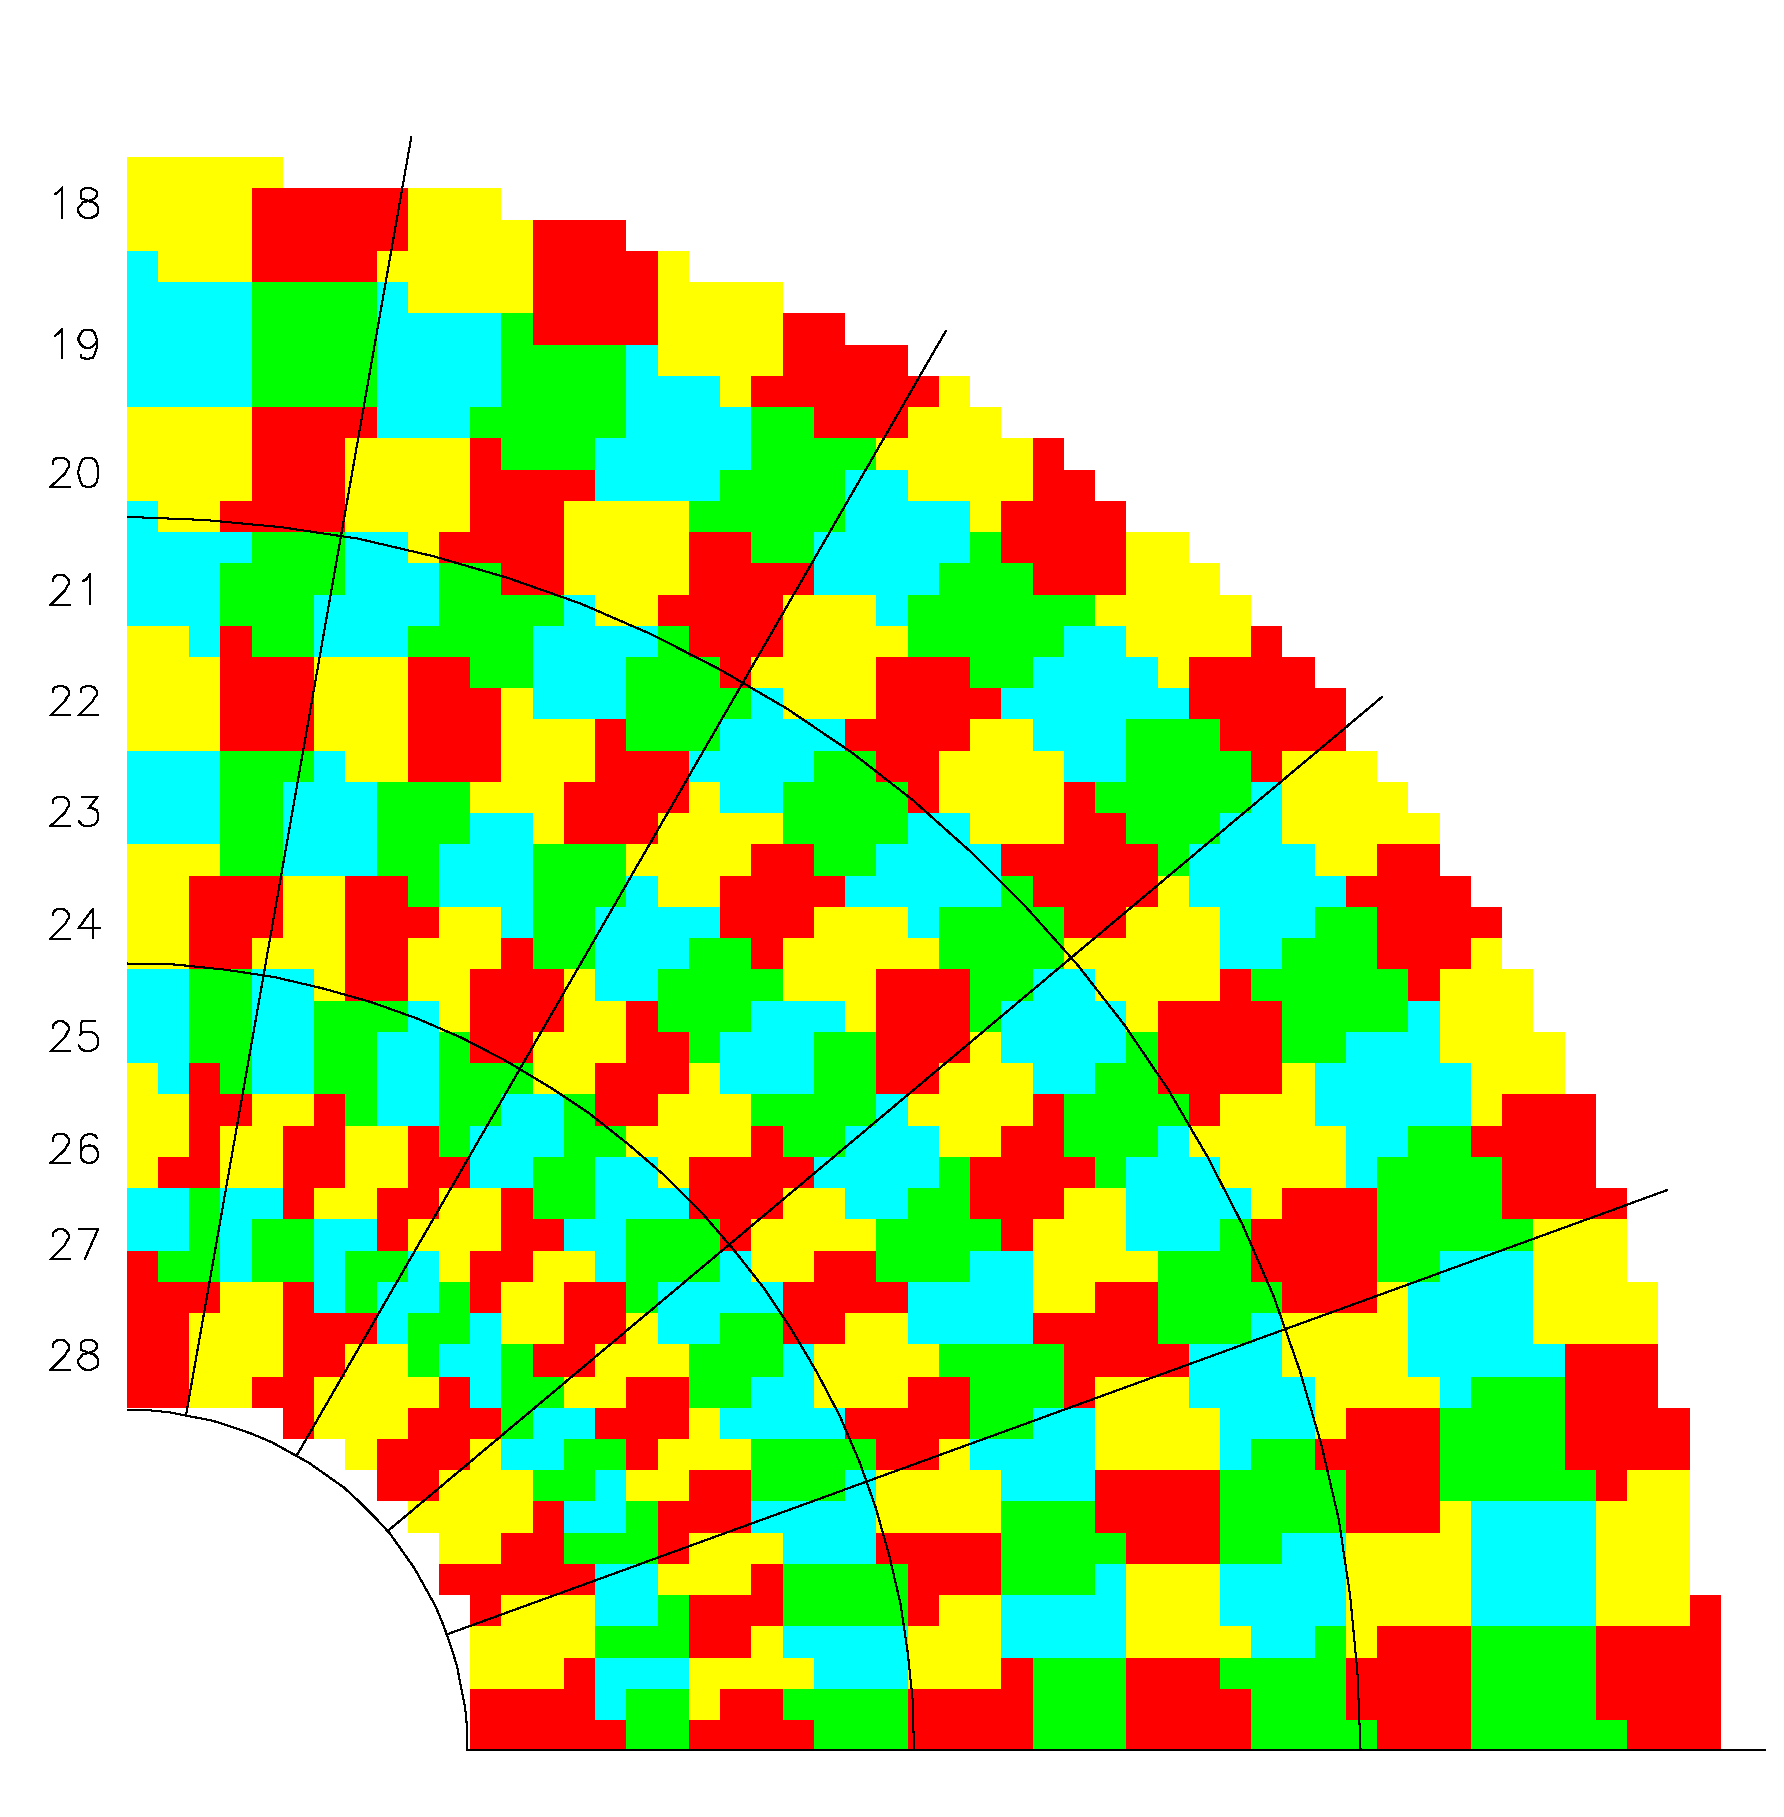
\includegraphics[width=0.4\linewidth]{Figures/L1TP/EE_L1TP.pdf}}
    \subfloat[]{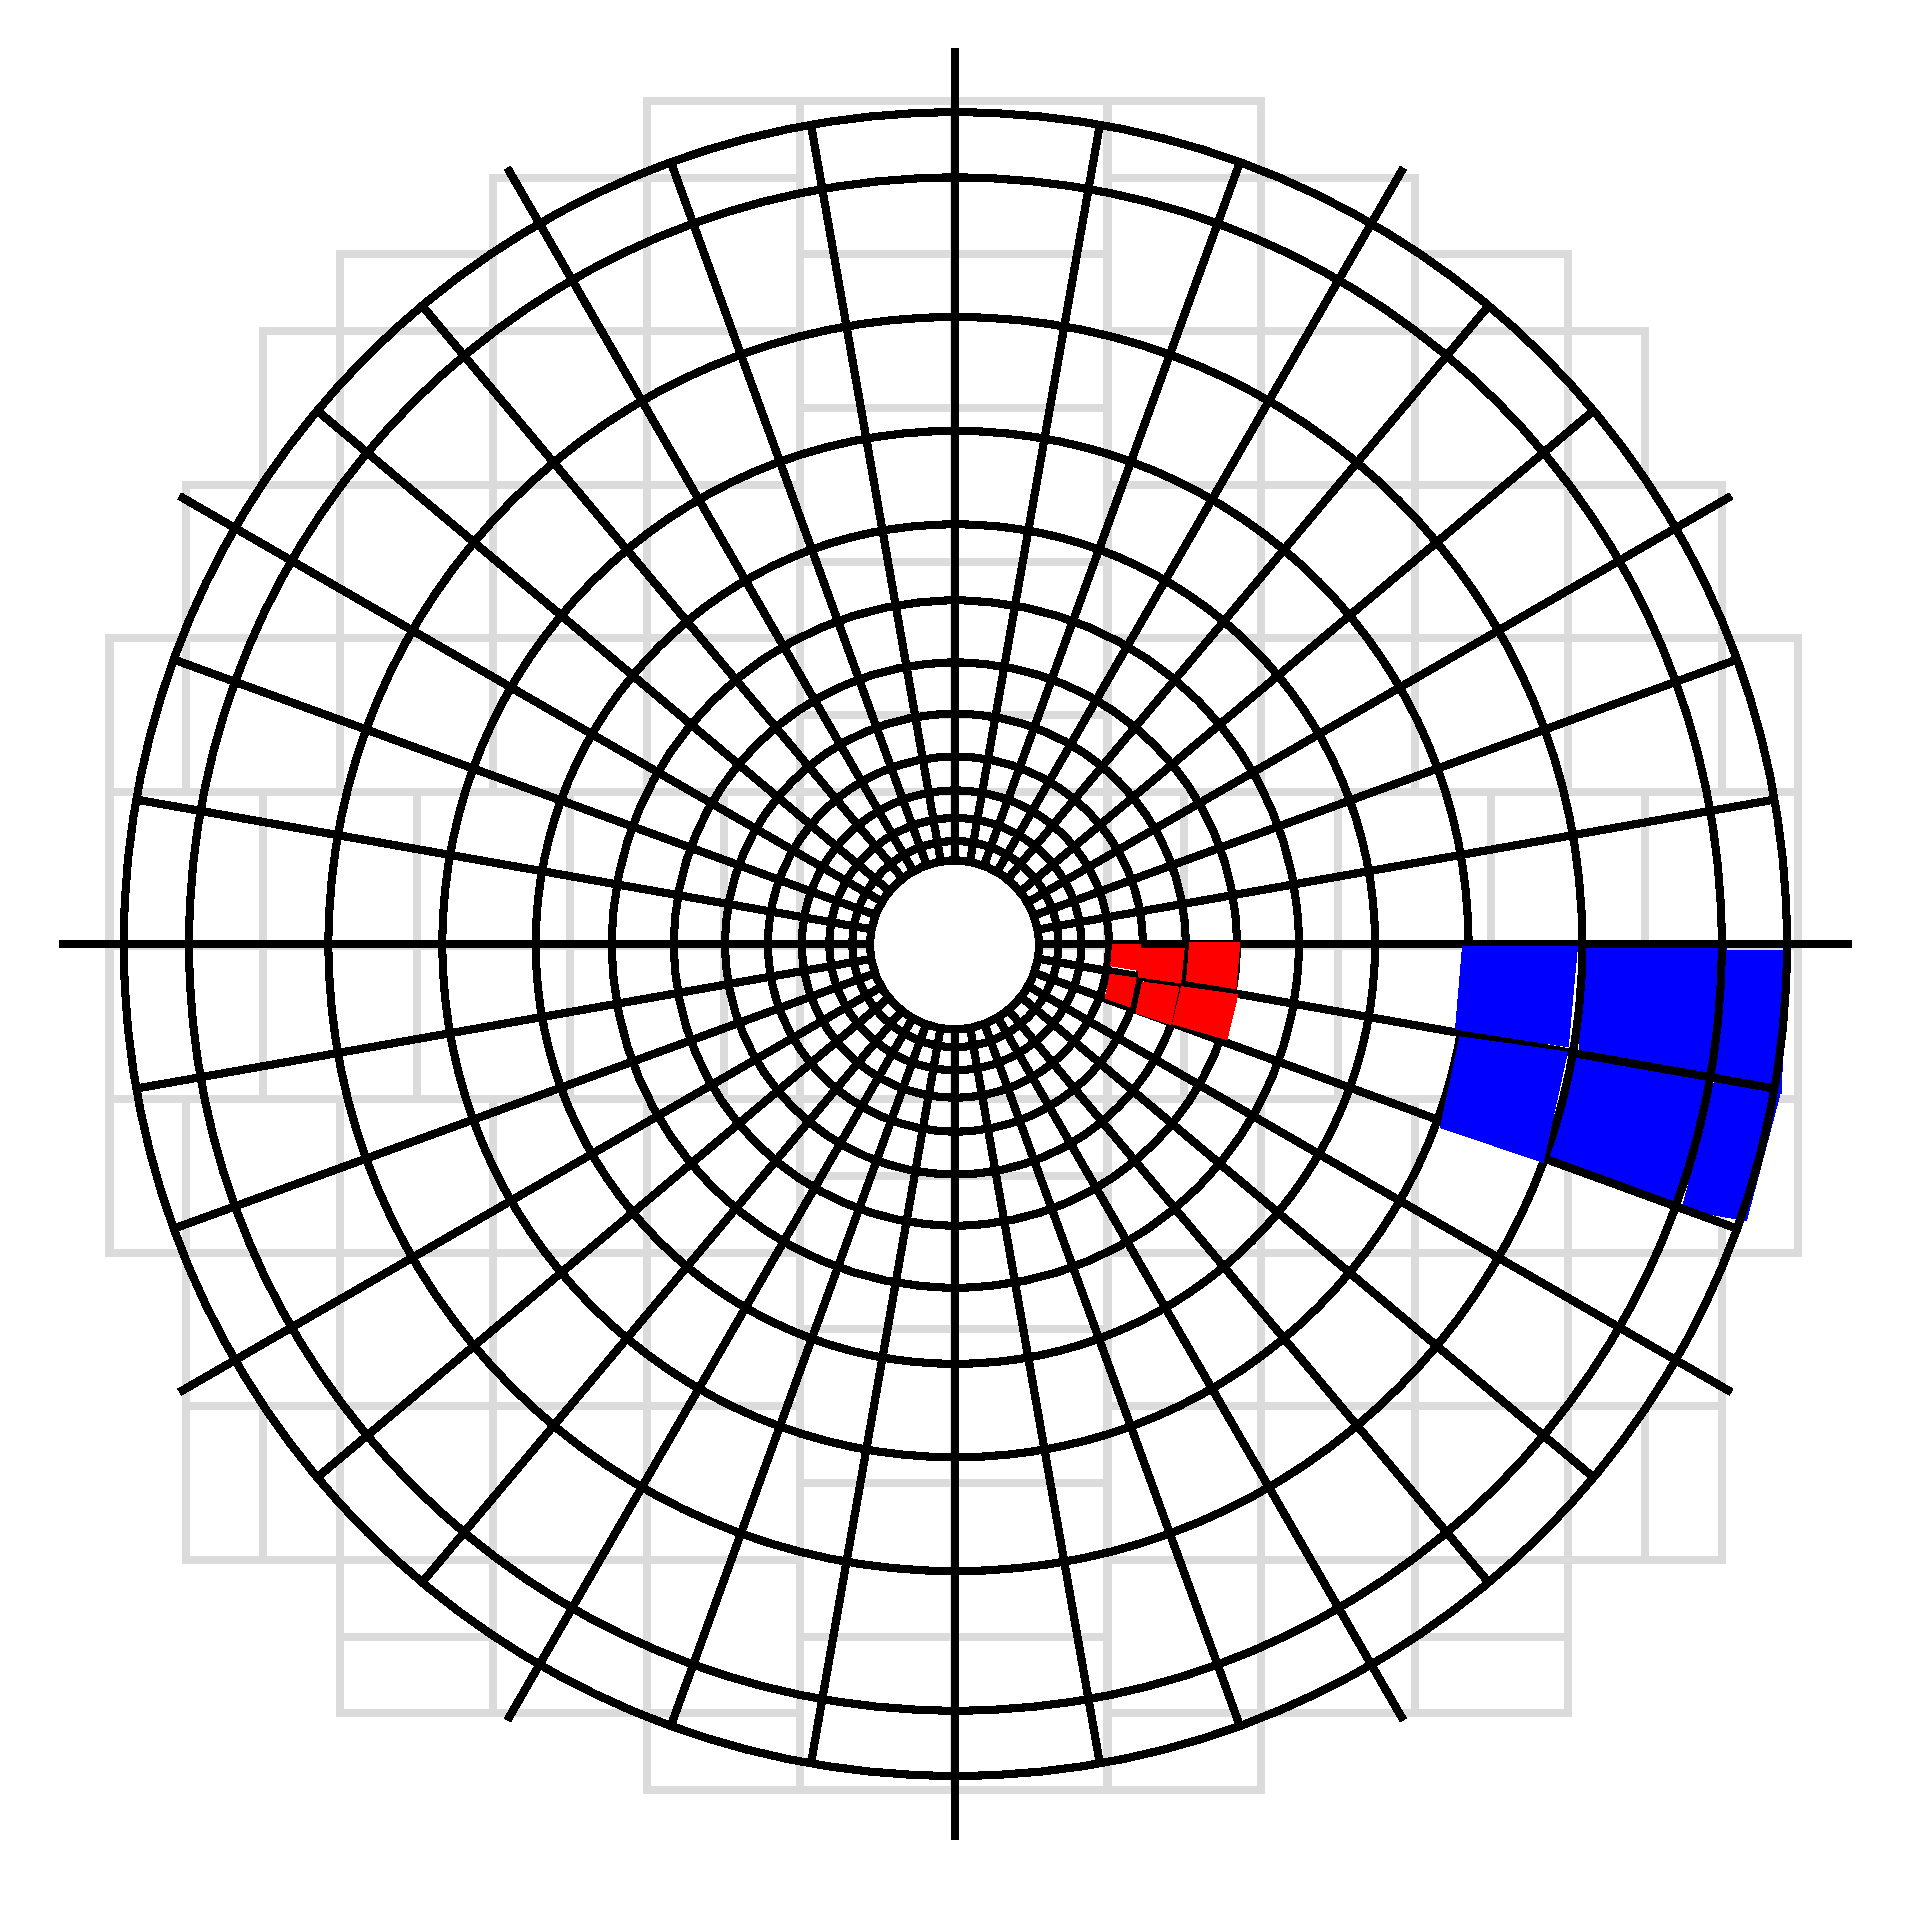
\includegraphics[width=0.4\linewidth]{Figures/L1TP/HF_L1TP.pdf}}
    \caption{Calorimeter Trigger Primitives (TP) layout in the x–y projection of the ECAL endcap (a); each square denotes a different ECAL crystal, and regions characterised by the same color represent one TP.
    Calorimeter TPs layout in the x–y projection of the HF detector (b); each square denotes a HF read-out unit, and regions with the same colour represent one Trigger Tower (TT).}
    \label{fig:EE_HF_L1TP}
\end{figure}

\begin{figure}
    \centering
    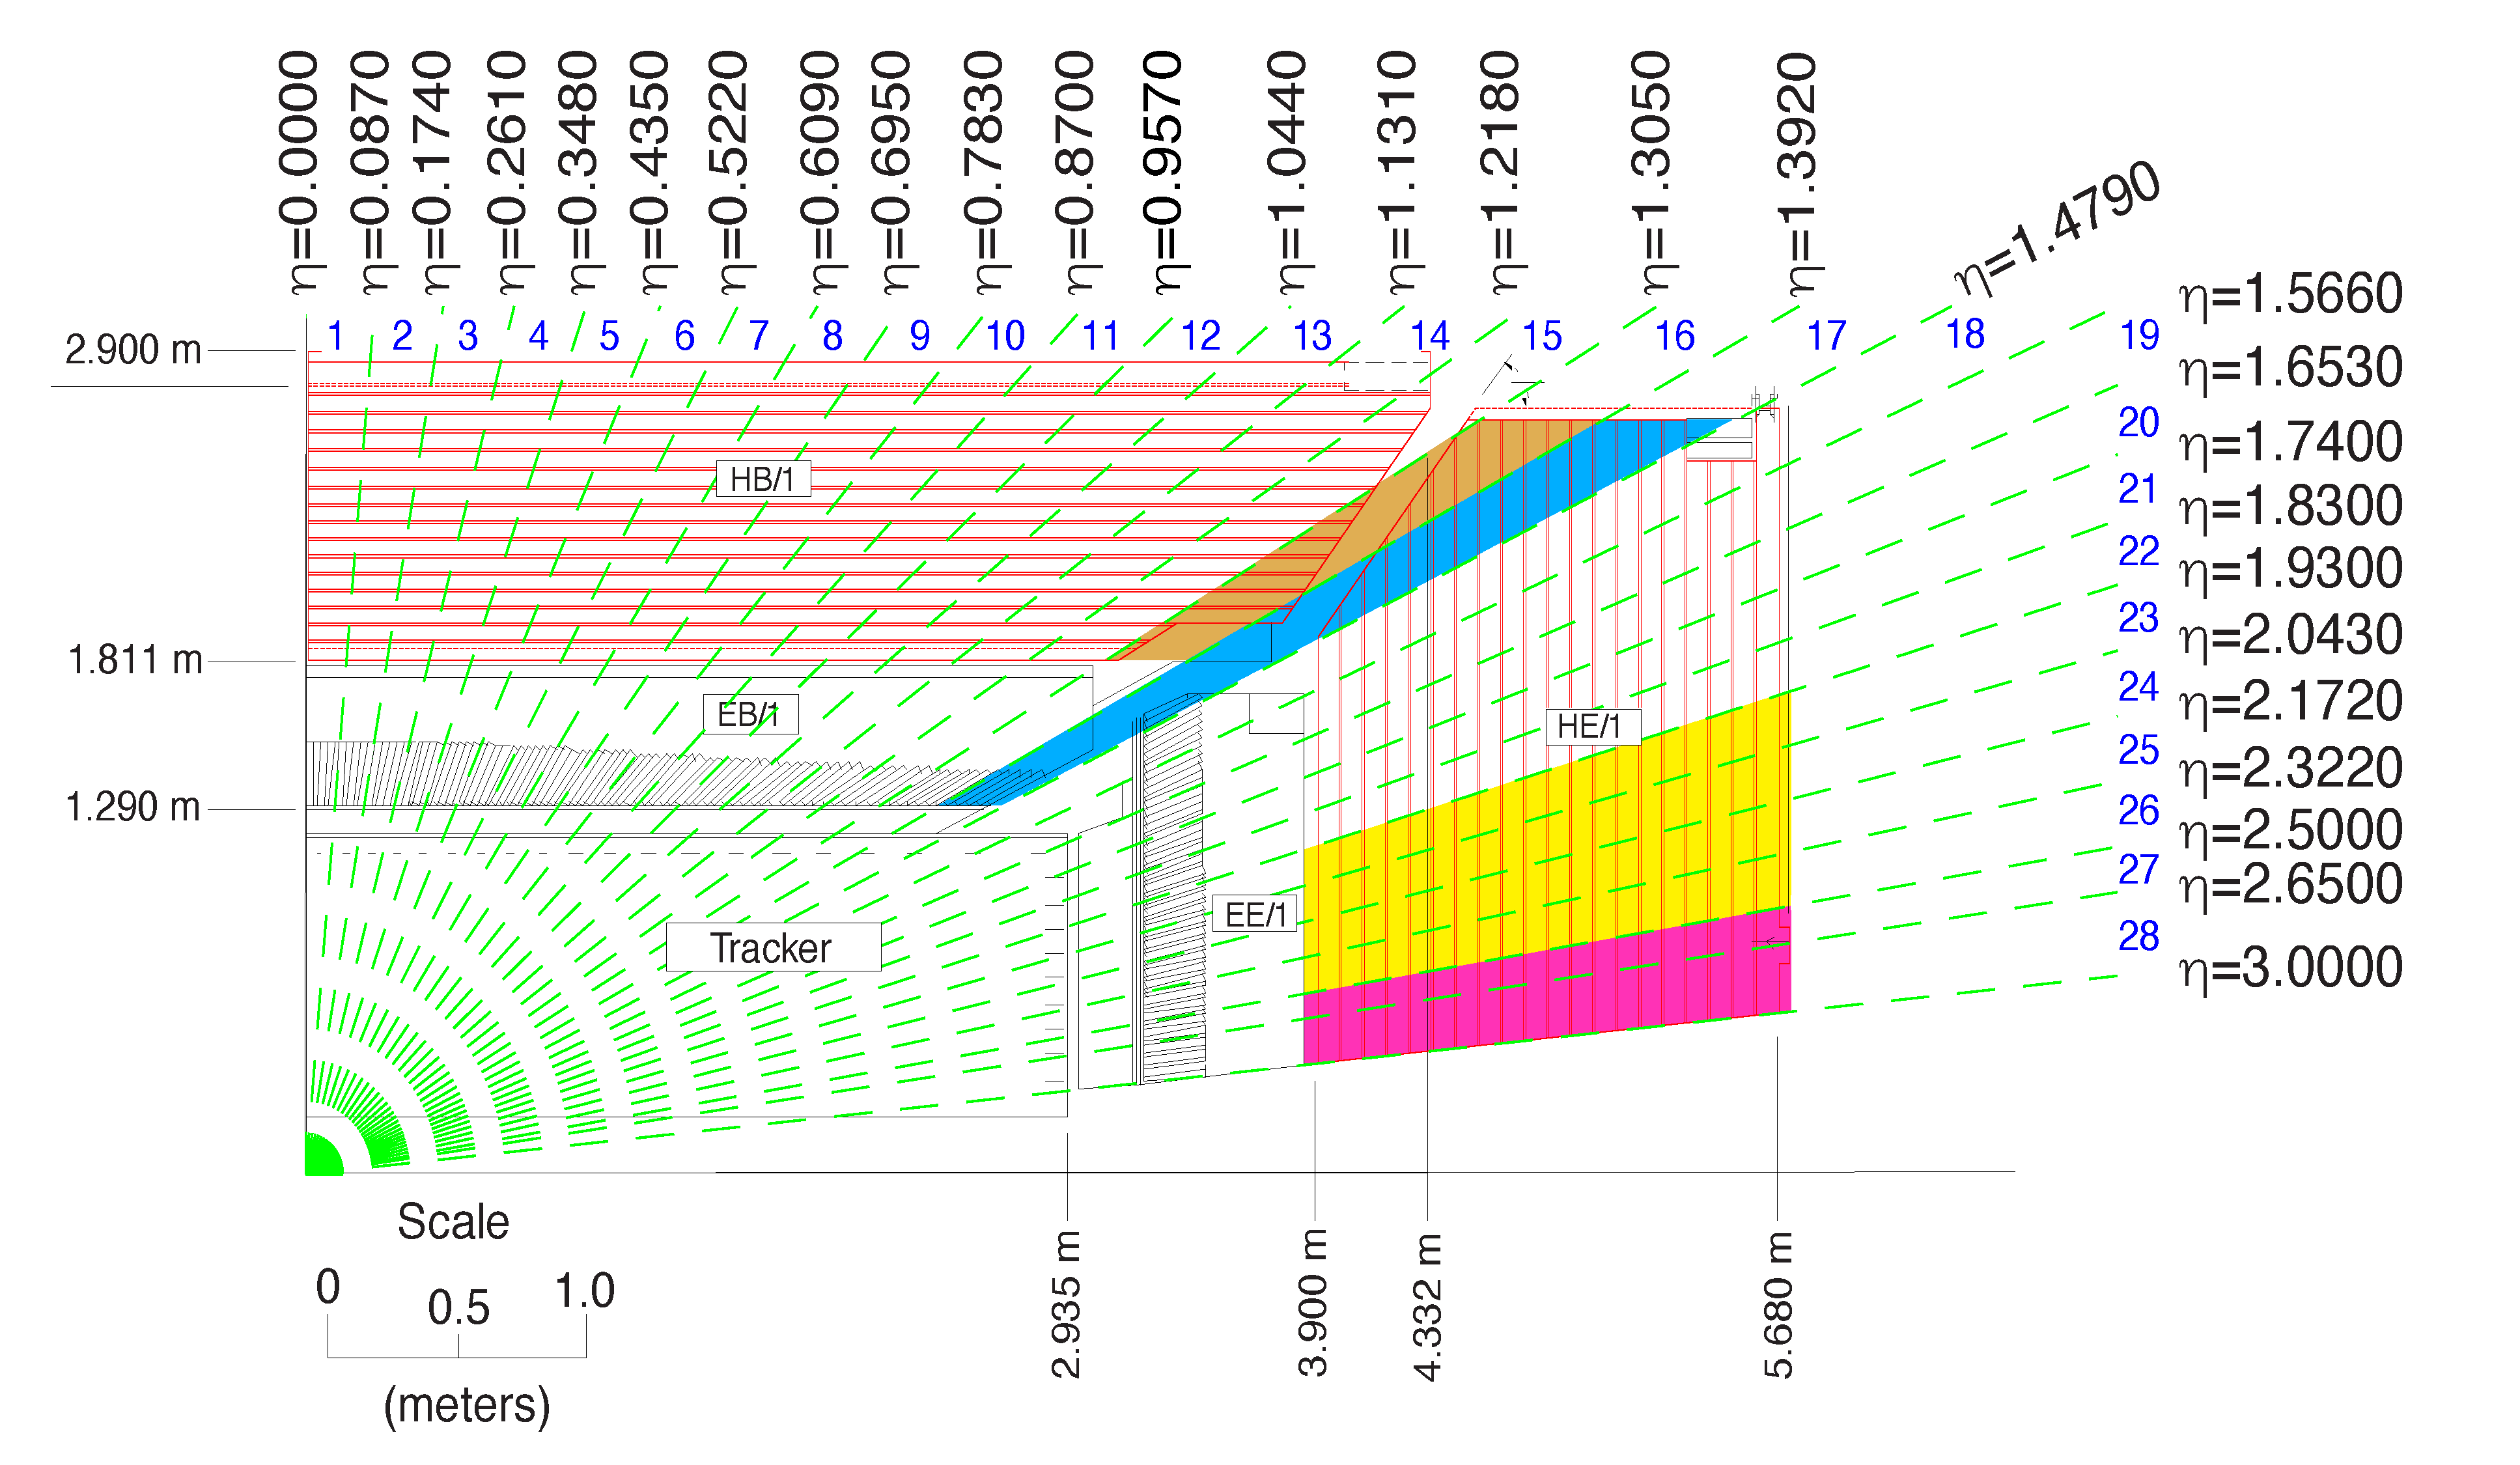
\includegraphics[width=0.9\linewidth]{Figures/L1TP/L1TP.pdf}
    \caption{Schematic view of the ECAL and HCAL TP separation in the $r$-$z$ projection of the CMS detector. }
    \label{fig:Layer1}
\end{figure}

\bigbreak

Each TP is characterised by a ($i\eta$, $i\phi$) position and a transverse energy, denoted as $E_T$.
The energy deposit is computed as the projection onto the transverse plane of the momentum vector originating in the detector centre and pointing to the calorimeter cells. This value is encoded into 8-bit digital quantities, corresponding to 256 possible values: each bit correspond to a 0.5~GeV unit, therefore each TP can transmit up to 127.5~GeV and higher values are saturated to the maximum.
The ($i\eta$, $i\phi$) position, instead, does not need to be encoded into digital quantities as it is fully determined by the linking in the detector read-out to the calorimeter trigger Layer-1.

The ECAL and HCAL TPs are transmitted to the Layer-1 calorimeter trigger, where a calibration factor is applied to each of them, based on position and energy deposit. Beside correcting for the detector non-homogeneity, the Layer-1 calibration can adjust the inter-calibration between the energy recorder in ECAL and HCAL TPs.
After the calibration, the ECAL and HCAL TPs that geometrically lie one behind the other are combined together into Trigger Towers (TTs).
A particular configuration is followed for the HF detector, where coarser TT granularity is adopted, with a segmentation of 4 TTs in $\eta$ and of 18 TTs in $\phi$ direction. 
Each TT is characterised by a 16-bit digital quantity that encodes a 9-bit word reporting the total $E_T$ from both ECAL and HCAL, the ratio of the ECAL and HCAL energies on 5 bits, and HCAL and ECAL quality flags on the 2 remaining bits.
At this stage, TTs can contain up to 255~GeV, and any TT with $E_T \geq 0.5$~GeV is referred to as an \textit{fired tower}. 
Finally, the Layer-1 sorts the TTs in descending $E_T$ order and transmits them to Layer-2, where any of the Master Processor (MP7) cards receives the complete set of TTs from each bunch crossing. 

\subsection{The Layer-2 calorimeter objects}
\label{subsec:The Layer-2 calorimeter objects}

In the Layer-2 calorimeter trigger, the TTs are merged together to form L1 objects. The L1 reconstruction algorithms have been developed and optimised to reconstruct electrons, photons, jets, hadronically decaying tau leptons, and energy sums.
Such algorithms need to access the full calorimeter information and require fast computing power furnished by Field-Programmable Gate Arrays (FPGAs) firmware.
A brief overview of the L1 calorimeter candidates reconstruction algorithms is given in the following paragraphs.

\subsubsection{Electrons and photon candidates}

Due to the unavailability of the tracking information at the L1 stage, electrons and photons are indistinguishable and grouped together in the $e/\gamma$ category, or \texttt{EGamma}.
The L1 $e/\gamma$ candidate is initiated by the presence of a high energy deposit in a single TT, also called \textit{seed}. The TTs around the seed are dynamically clustered~\cite{Sauvan_2015} to the seed according to their position and recorded energy.
The maximum cluster size is limited to 8 TTs, in order to minimise the impact of pile-up energy deposits while including most of the electron or photon energy.
Since electron and photon showers spread mostly along the $\phi$ direction due to the CMS magnetic field, an extended region in $\phi$ (5 TTs at most) and narrow in $\eta$ (2 TTs at most) is chosen.
The first and second neighbour fired TTs are clustered only if connected to the seed, as shown in Figure~\ref{fig:L1EGammaCluster}~(left).
The dynamic clustering leads to a large variety of cluster shapes depending on the distribution of the energy around the seed tower. Large clusters involving many trigger towers are probably produced by the pre-showering of jets in ECAL, while small clusters, containing typically one to four TTs, are more compatible with electron or photon showers. For this reason, the shape of the cluster, which would not be available for a fixed size clustering, is an important information for the particle candidate and brings additional discrimination power between electrons (or photons) and jets.

The sum of the ECAL $E_T$ of the seed and clustered towers is considered the raw $E_T$ of the $e/\gamma$ cluster, which is calibrated using Layer-2 scale factors dependent on the $\eta$-position of the seed tower. These calibration factors, derived from $Z \rightarrow ee$ events, are defined as the ratio of the offline reconstructed electron $E_T$ to the corresponding raw L1 cluster $E_T$.
Since the Layer-2 calorimeter trigger has access to TTs without boundaries, it is possible to account for the pile-up conditions by applying isolation requirements. The isolation energy is computed in a $5\time9$ TTs region, excluding the $e/\gamma$ candidate footprint in ECAL ($2\times5$ TTs) and HCAL ($1\times2$ TTs). The isolation region is better illustrated in Figure~\ref{fig:L1EGammaCluster}~(right). The isolation threshold depends on the $i\eta$ position of the cluster and on an estimator for the number of pile-up interactions, given by the number of TTs in the whole detector acceptance recording an energy $E_T>4$~GeV. 
Finally, an energy-dependent threshold on the ration between ECAL and HCAL energy deposit, also known as $E/H$, is applied to reduce the mis-identification rate of hadronic showers.

\begin{figure}
    \centering
    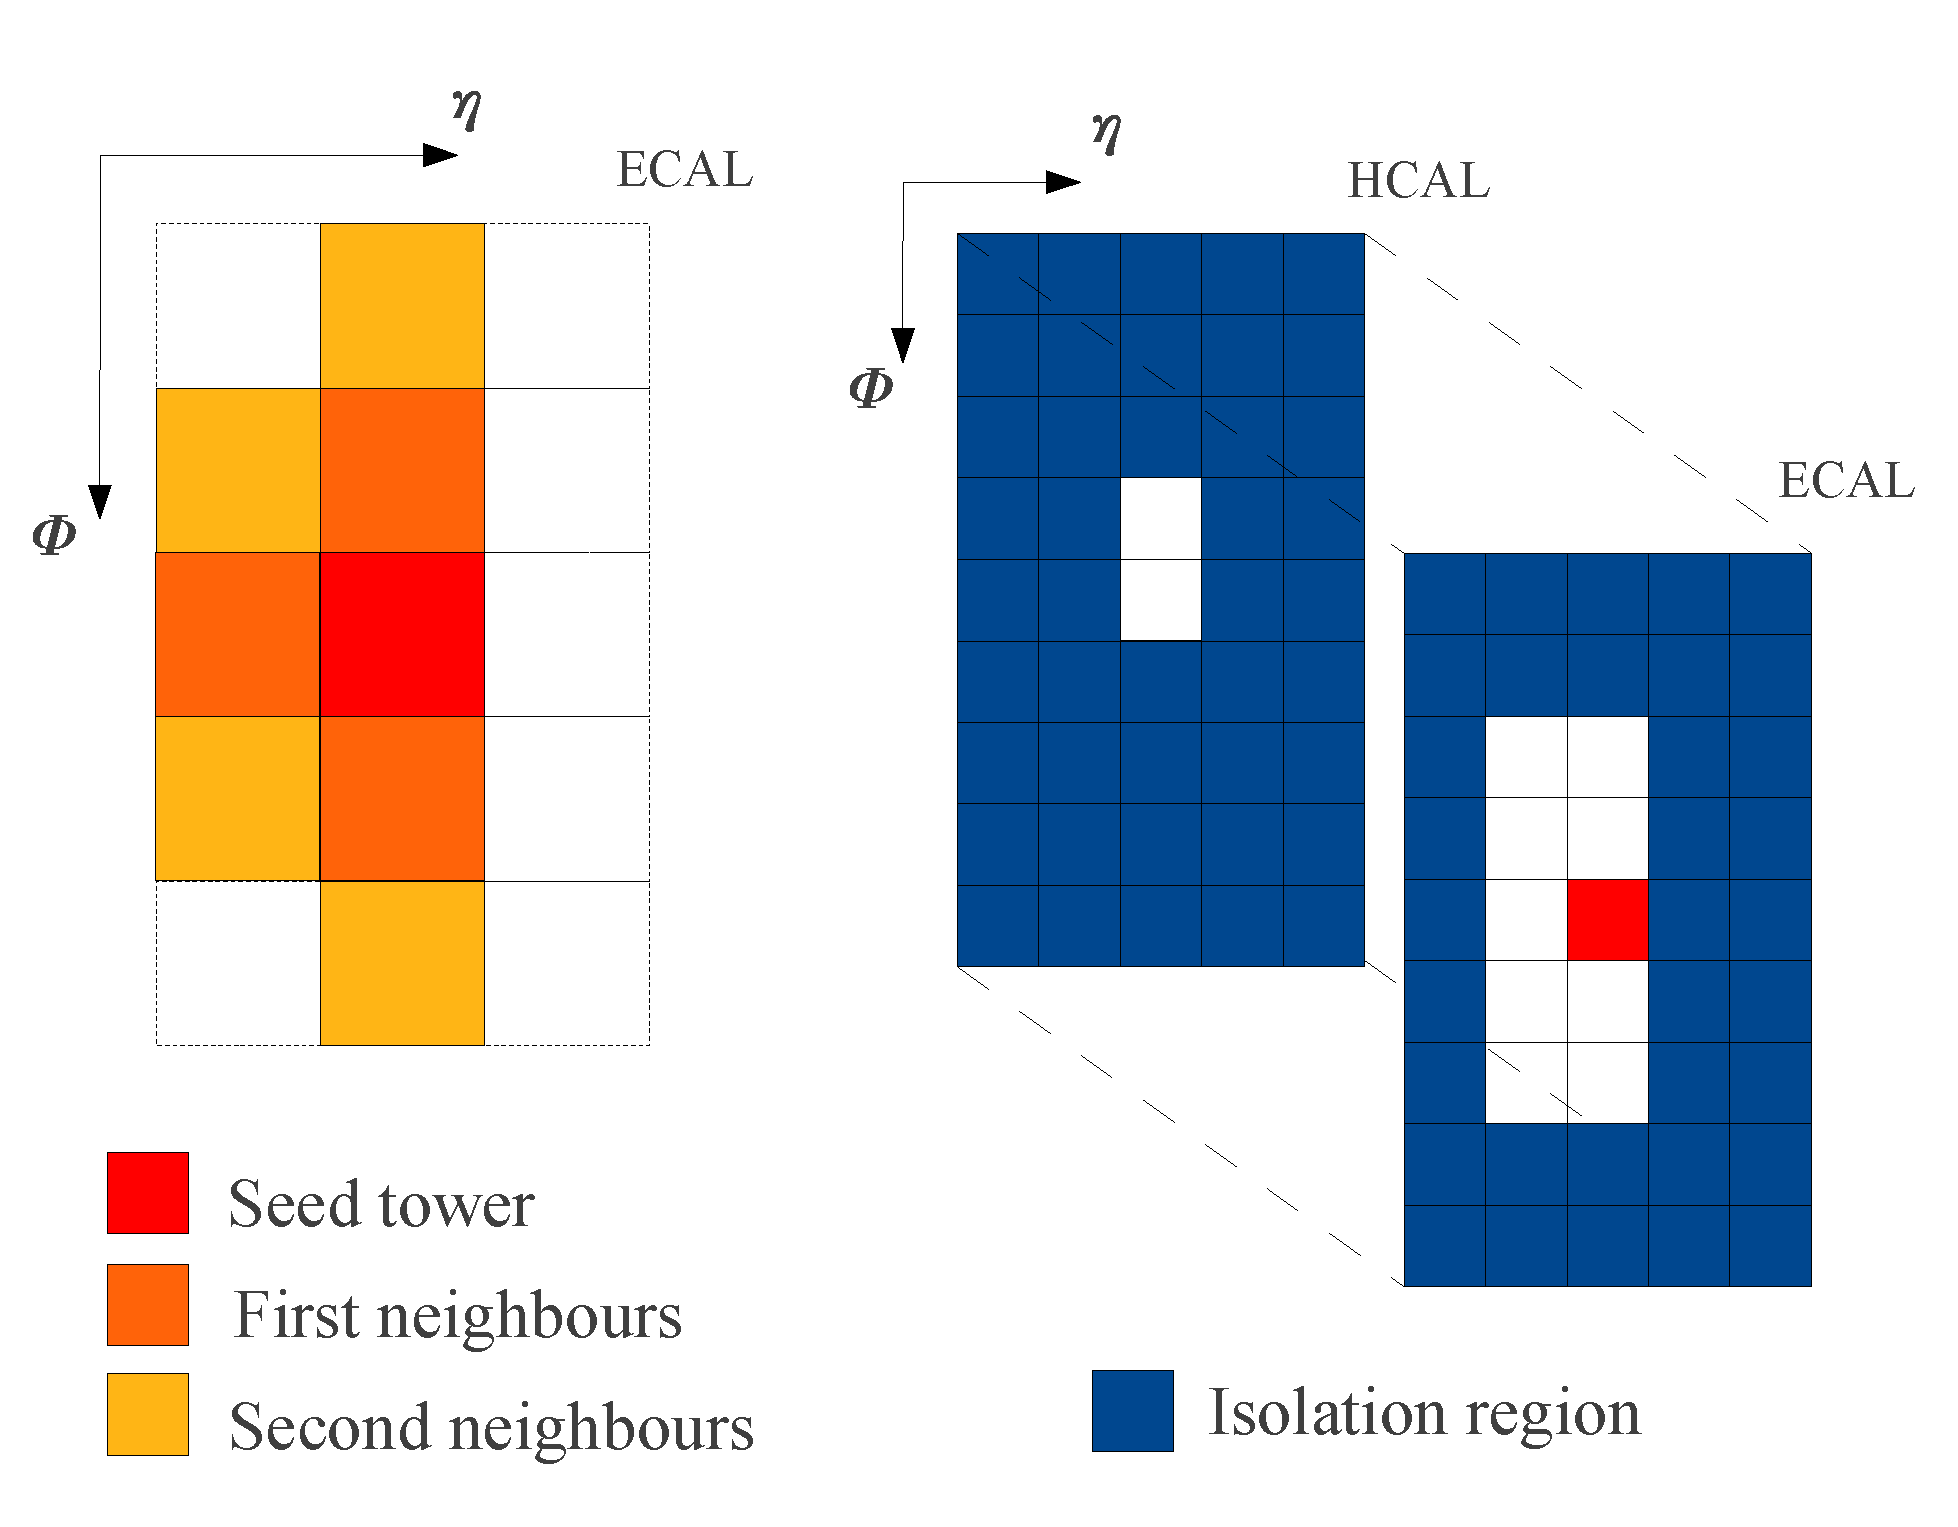
\includegraphics[width=0.5\linewidth]{Figures/L1TP/L1EGammaCluster.pdf}
    \caption{Schematic for the L1 $e/\gamma$ dynamic clustering and isolation. A candidate is formed by clustering around the seed all the fired neighbour towers. A candidate is considered as isolated if the $E_T$ in the ECAL and HCAL isolation regions is smaller than a given value.}
    \label{fig:L1EGammaCluster}
\end{figure}

\subsubsection{Hadronic tau lepton candidates}

Hadronically decaying $\tau$ leptons are reconstructed by the Layer-2 calorimeter trigger with an algorithm similar to the one used for $e/\gamma$ candidates.
The most probable products for the tau leptons hadronic decay are pions, which can leave energy deposit both in the ECAL and the HCAL calorimeters. 
The $\tau_h$ candidate selection begins a single TT seed, and the TTs around the seed, in a region spanning 5 and 9 TTs in the $\eta$ and $\phi$ directions respectively, are merged following the dynamic cluster procedure.
The TTs within one unit in $i\eta$ and $i\phi$ from the seed, and the ones on the same $i\eta$ position at two units distance in $i\phi$, are incorporated into the \textit{proto-cluster}. A subsequent \textit{lateral trimming} procedure is implemented to remove the least energetic side of the proto-cluster, as shown in Figure~\ref{fig:L1TauCluster}~(left).

Since the $\tau_h$ decay can produce several charged or neutral pions, leading to broader energy deposit. 
For this reason, at the same as the primary proto-cluster creation, \textit{secondary clusters} are built with the same approach, but considering a smaller window spanning 3 TTs in both $\eta$ and $\phi$ directions.
The secondary clusters are merged to the primary proto-cluster only if their seed is found in one of the eight positions highlighted in green in Figure~\ref{fig:L1TauCluster}~(right). An overlap procedure is applied to avoid double-counting of TTs in multiple clusters.
The sum of all the TTs $E_T$ included in the merged cluster is considered to be the raw $E_T$ of the $\tau_h$ cluster, which is calibrated using Layer-2 scale factors dependent on raw energy deposit, the $\eta$-position of the seed tower, the presence of ECAL energy deposit, and the cluster being issued by the merging procedure or not.
Also for $\tau_h$ candidates, an isolation requirement is applied to reduce contamination from hadronic jets, characterised by wider calorimeter activity. The isolation energy is computed in a $6\time9$ TTs region, excluding the $\tau_h$ candidate footprint.
The isolation threshold depends on the raw energy deposit, on the $i\eta$ position of the cluster, and on an estimator for the number of pile-up interactions, given by the number of fired TTs in the most central region of the barrel, i.e. $|i\eta|\leq 4$.

\begin{figure}
    \centering
    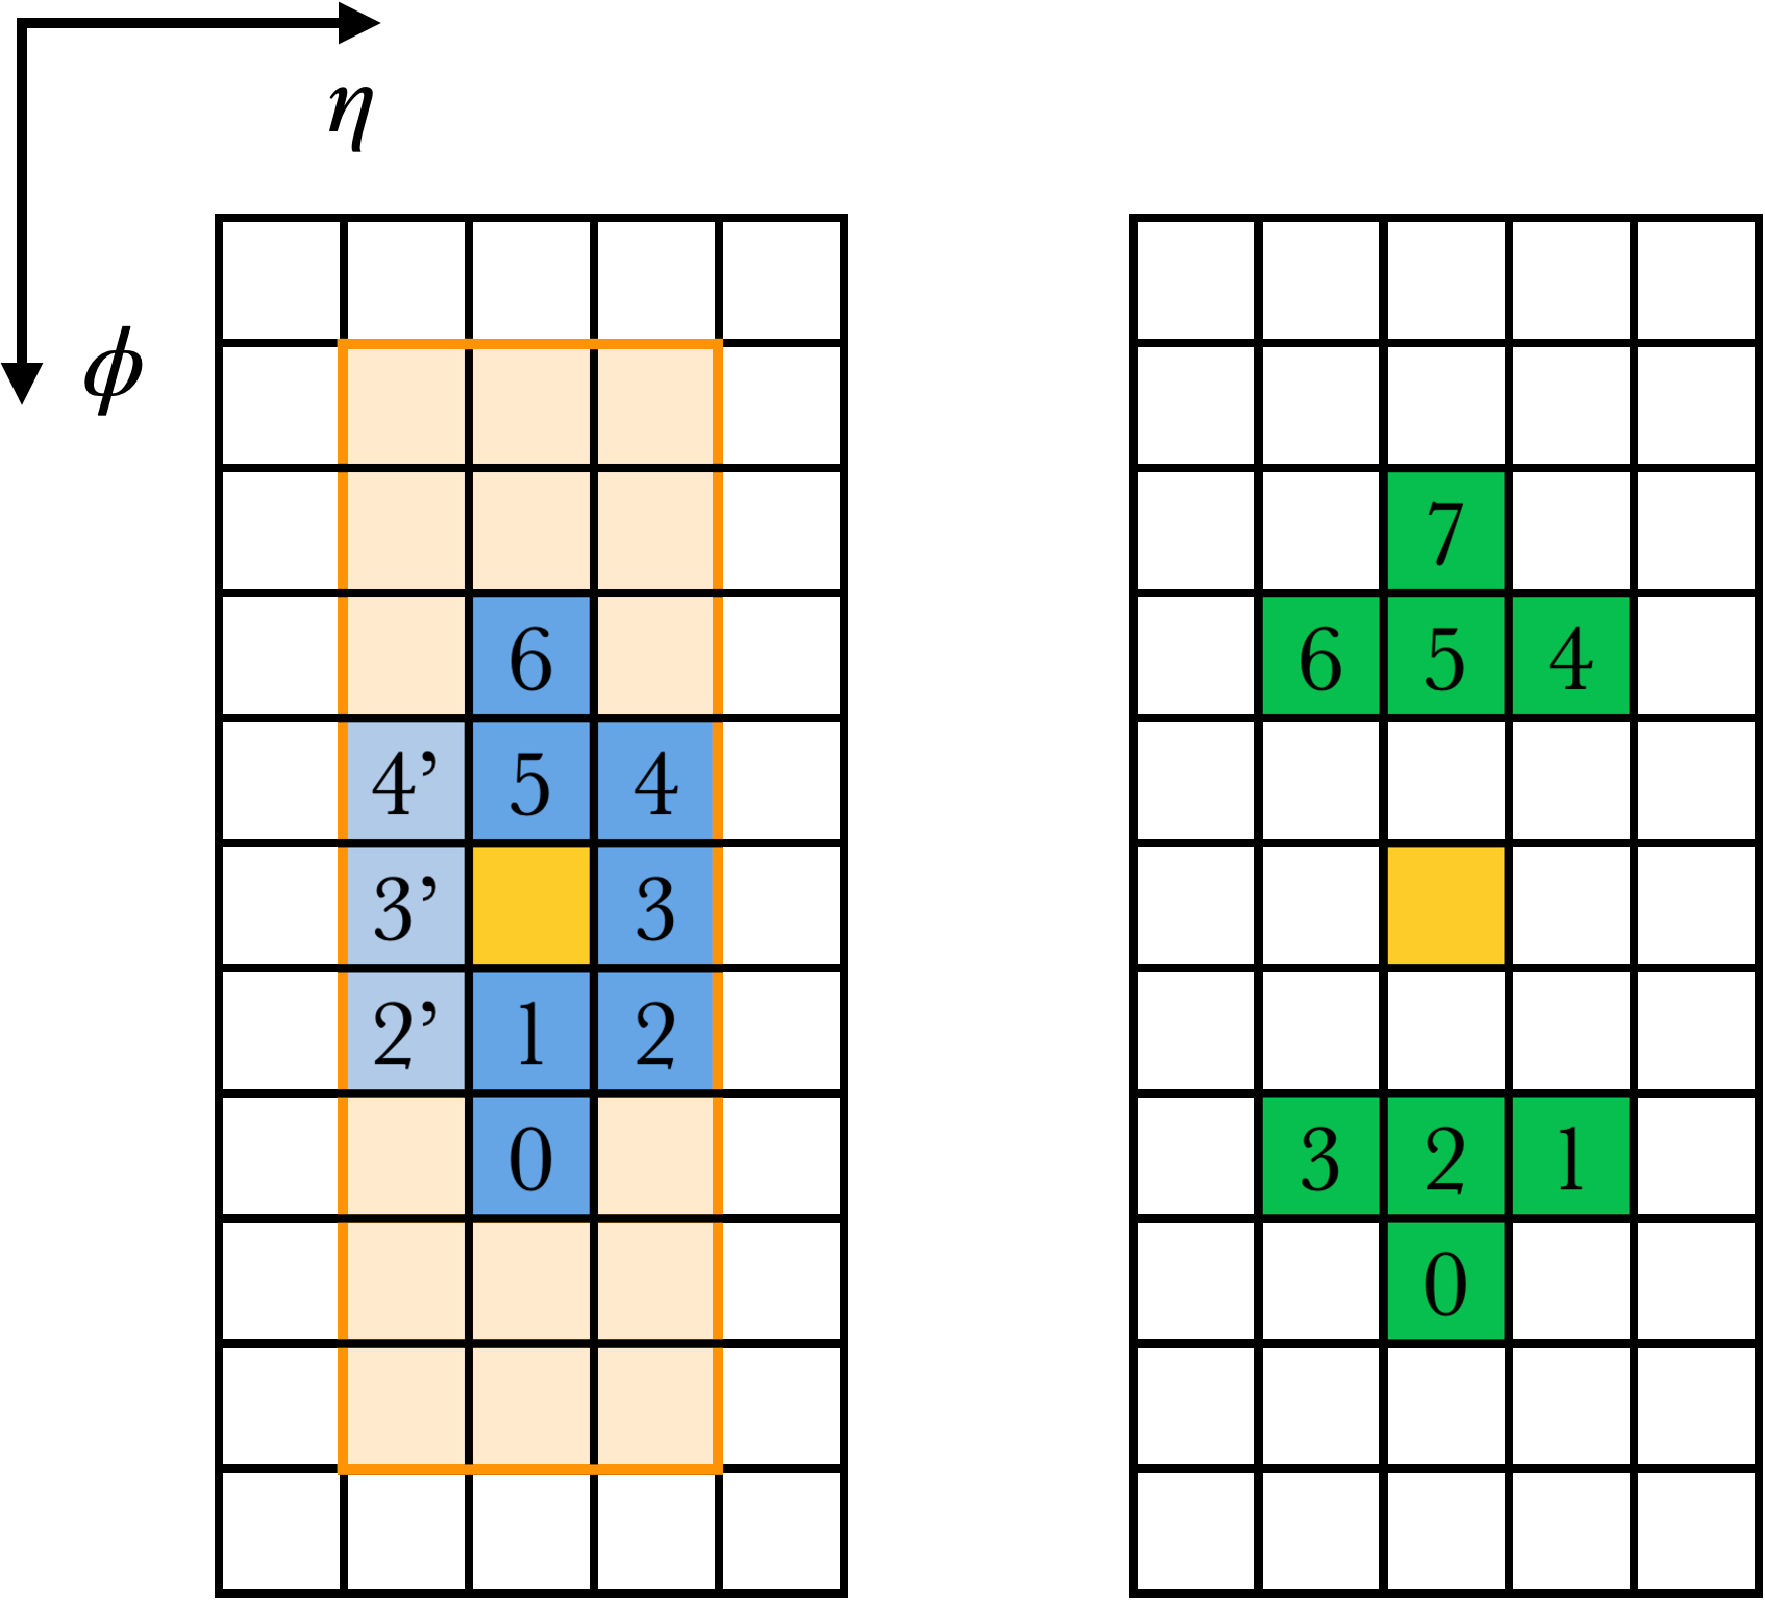
\includegraphics[width=0.4\linewidth]{Figures/L1TP/L1TauCluster.pdf}
    \caption{Schematic for the $\tau_h$ dynamic clustering algorithm. A candidate is initiated by the definition of a proto-clustering, consequently trimmed to remove the least energetic side (left). Additional secondary clusters can be merged to the primary one, if their seed lies within the seven green TTs (right); the secondary clusters seeded in position 2 or 5 are not considered if their seed is already included in the primary proto-cluster.}
    \label{fig:L1TauCluster}
\end{figure}

\subsubsection{Jet candidates}

The hadronic jet candidates are defined from a fixed dimension clustering approach. 
The L1 jet candidate is initiated by the presence of a high energy deposit in a single TT seed, and the surrounding matrix of $9\times9$ TTs defines as the jet cluster. 
The size of the window is chosen to correspond to the $\Delta R = 0.4$ angular opening, which is radius used for the offline anti-$k_T$ reconstruction algorithm~\cite{Zabi_2016}.
In order to avoid double counting of jets, a jet candidate is discarded if any of the TTs composing the cluster has an energy deposit greater than the central seed.
The energy in the $9\times9$ cluster, also known as \textit{chunky donut}, is defined to be the raw jet energy.

Given the large extension of the jet candidate, a dedicate pile-up subtraction method is implemented, which estimates the energy deposit due to pile-up and subtracts it to the jet raw energy deposit.
Two techniques for local pile-up correction are available in the Layer-2 algorithm employed during Run~III data taking:
\begin{itemize}
    \item Chunky donut subtraction: the pile-up energy is estimated as the sum of the energy deposit in the four $9\times3$ strips around the chunky donut, removing the highest and lowest energy sides.
    \item Phi-ring subtraction: the pile-up energy is estimated as the energy deposit on 9 rings of TTs with the same $\eta$ coordinates, re-scaling the surface to the $9\times9$ of the jet candidate.
\end{itemize}

As a last step, the Layer-2 jet candidates are calibrated based on their raw energy and $\eta$ position.

\begin{figure}
    \centering
    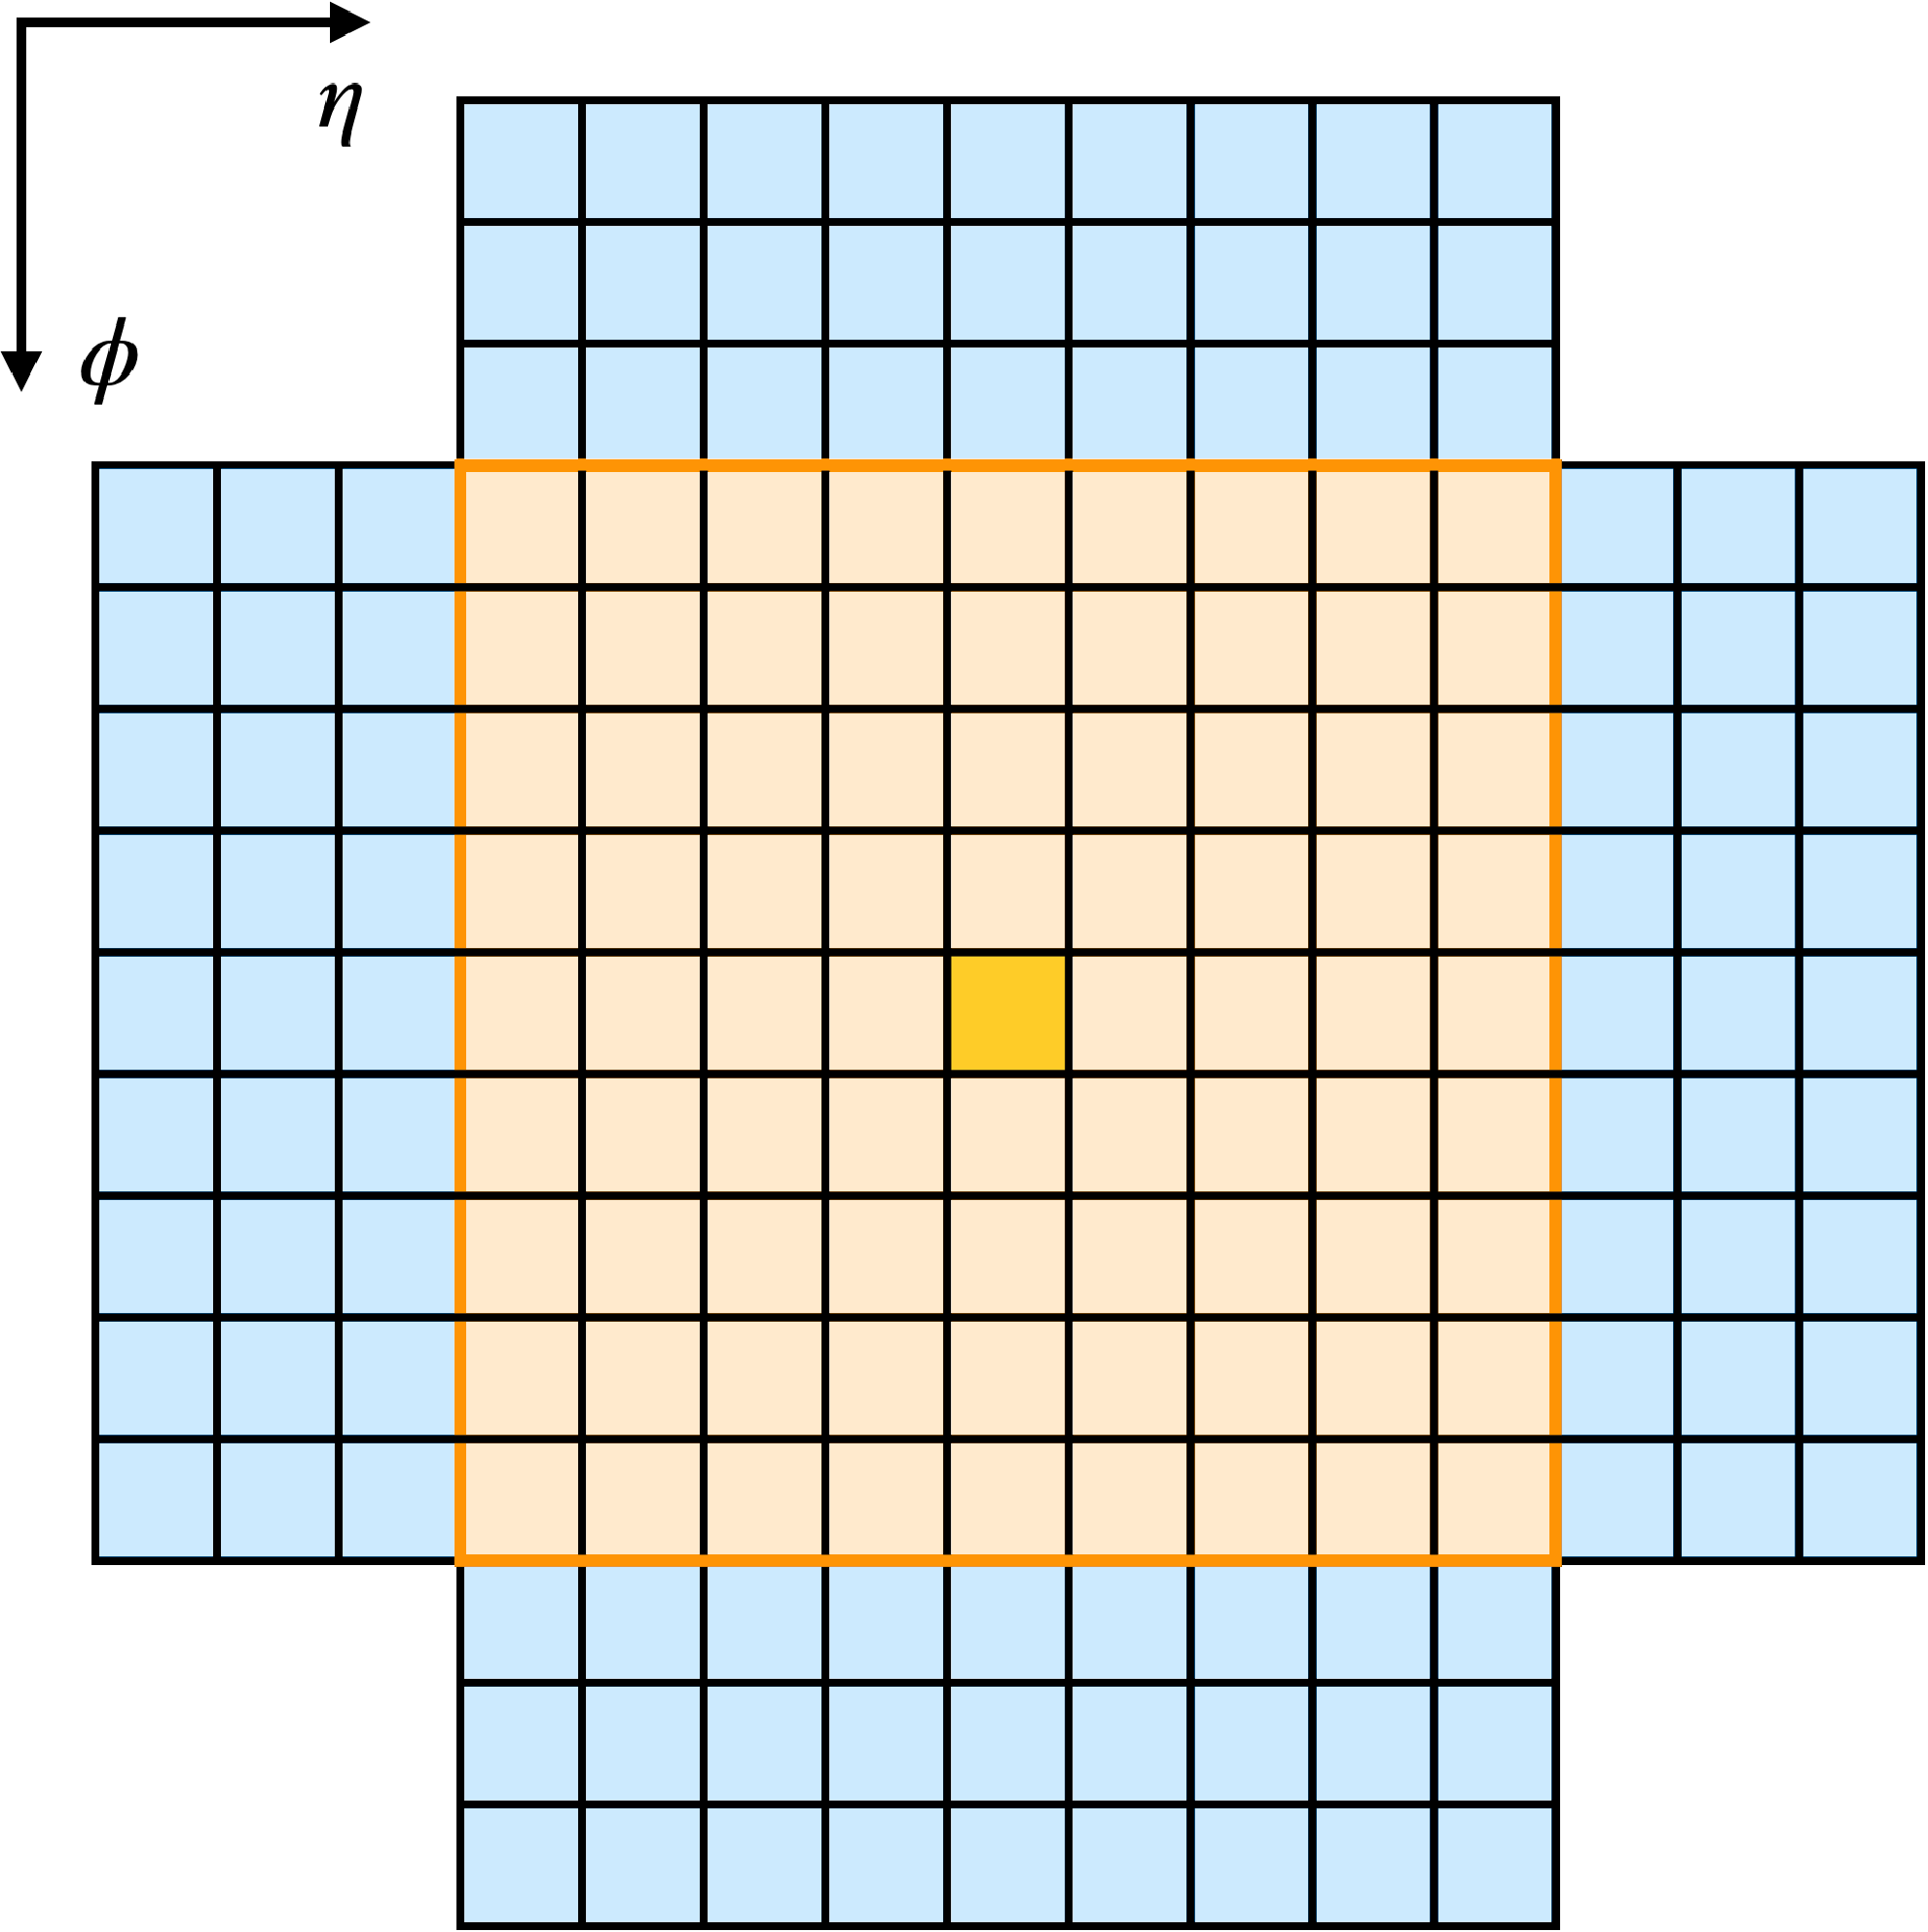
\includegraphics[width=0.4\linewidth]{Figures/L1TP/L1JetCluster.pdf}
    \caption{Schematic for the jet $9\times9$ chunky donut cluster. The four calorimeter strips around the chunky donut are used to estimate the local energy density due to piel-up.}
    \label{fig:L1JetCluster}
\end{figure}

\subsubsection{Energy sums candidates}

The energy sums are the last objects to be constructed in the L1 calorimeter trigger, as they involve full calorimeter granularity.
The total missing transverse energy $E_T^{miss}$ is computed by splitting the regional TTs energies into their $x$ and $y$ components, and summing the components in quadrature.
The resulting vector, after a rotation of $180^{\circ}$, provides the magnituse and angle of the missing energy due to neutrinos not interacting with the detector material.
The total scalar transverse energy of all jets $H_T$ is given by the sum over all clustered jets found in the event.
A dedicated pile-up subtraction and calibration is applied to $E_T^{miss}$ candidate to remove the large contribution coming from soft, diffuse pile-up energy deposits.
The pile-up contribution is estimated from the tower activity in the central part of the barrel and 

\begin{figure}
    \centering
    \subfloat[]{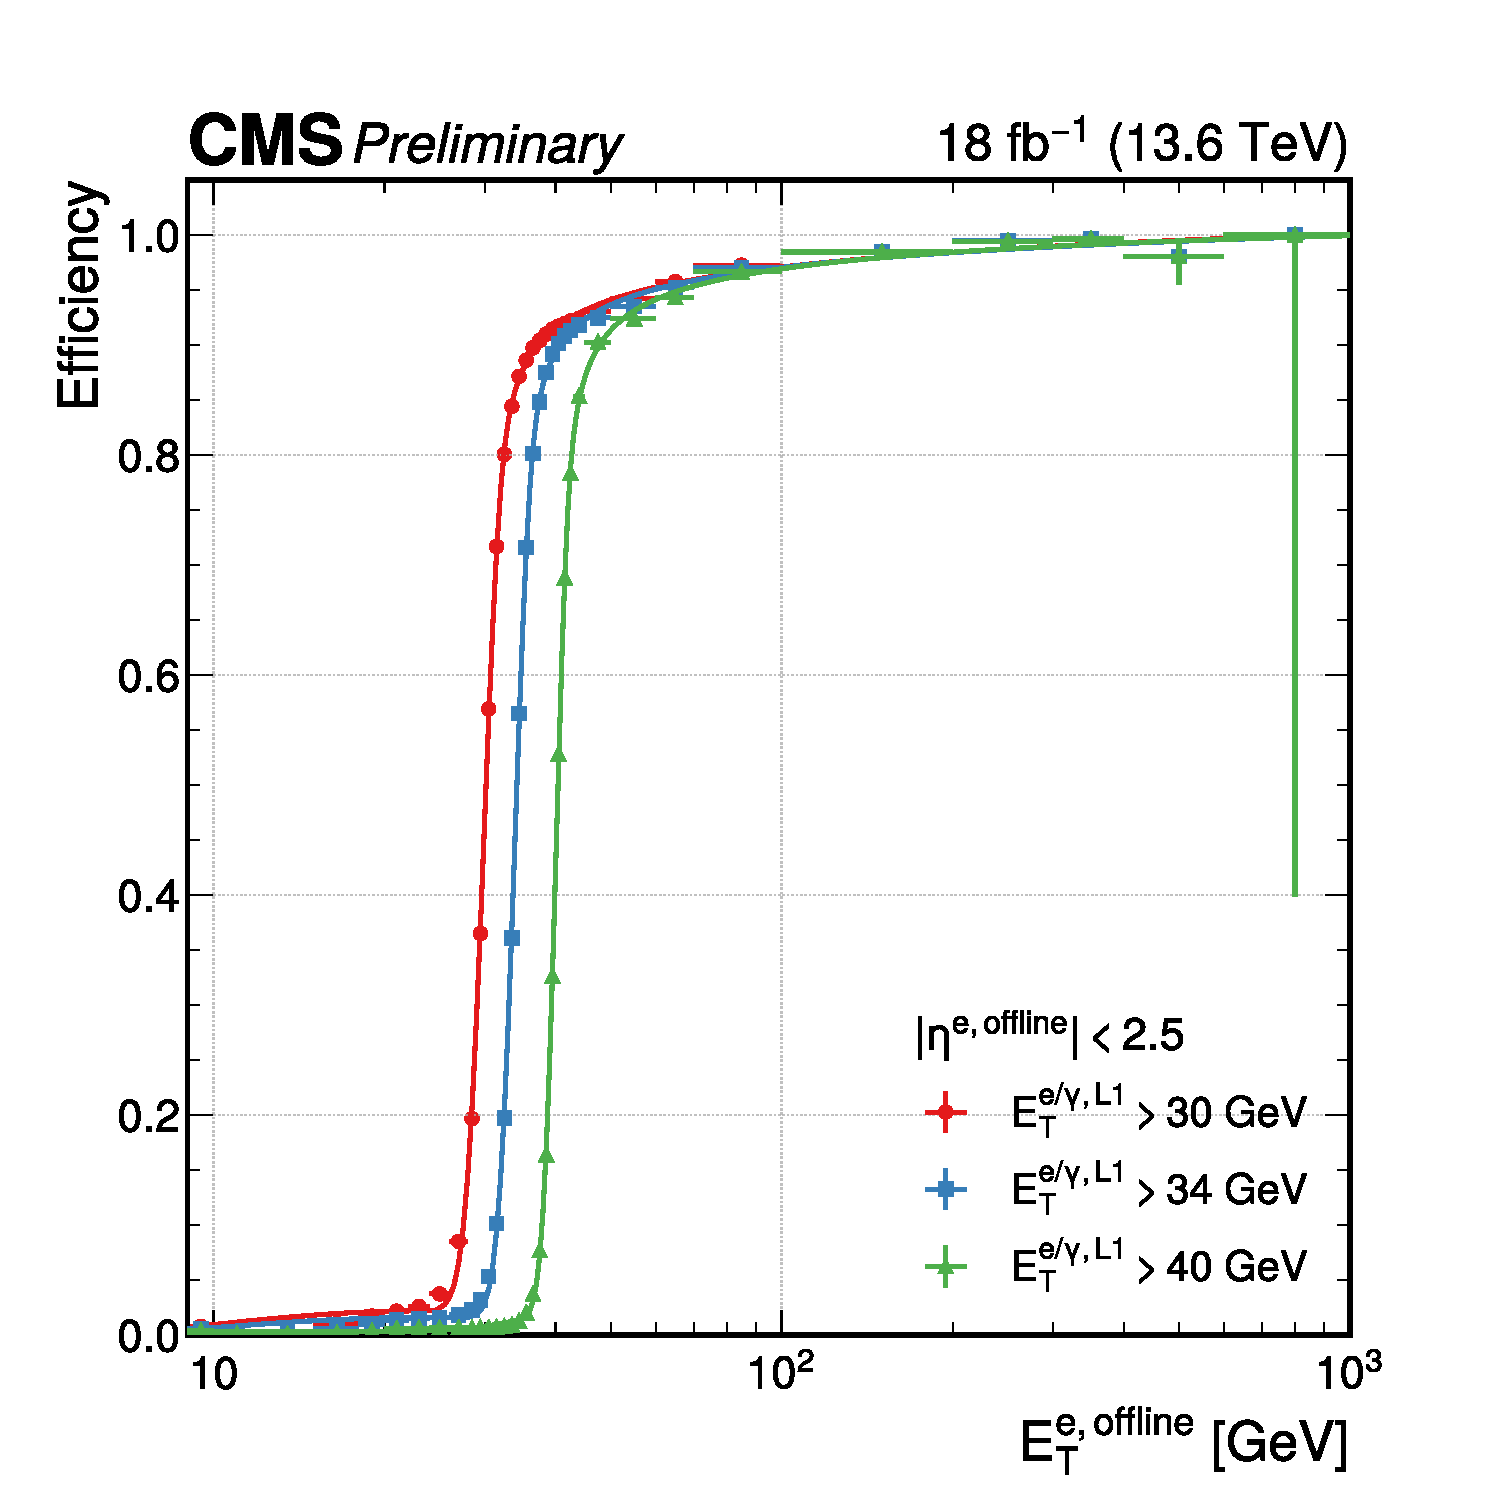
\includegraphics[width=0.4\linewidth]{Figures/L1TP/EGEfficiency.pdf}}
    \subfloat[]{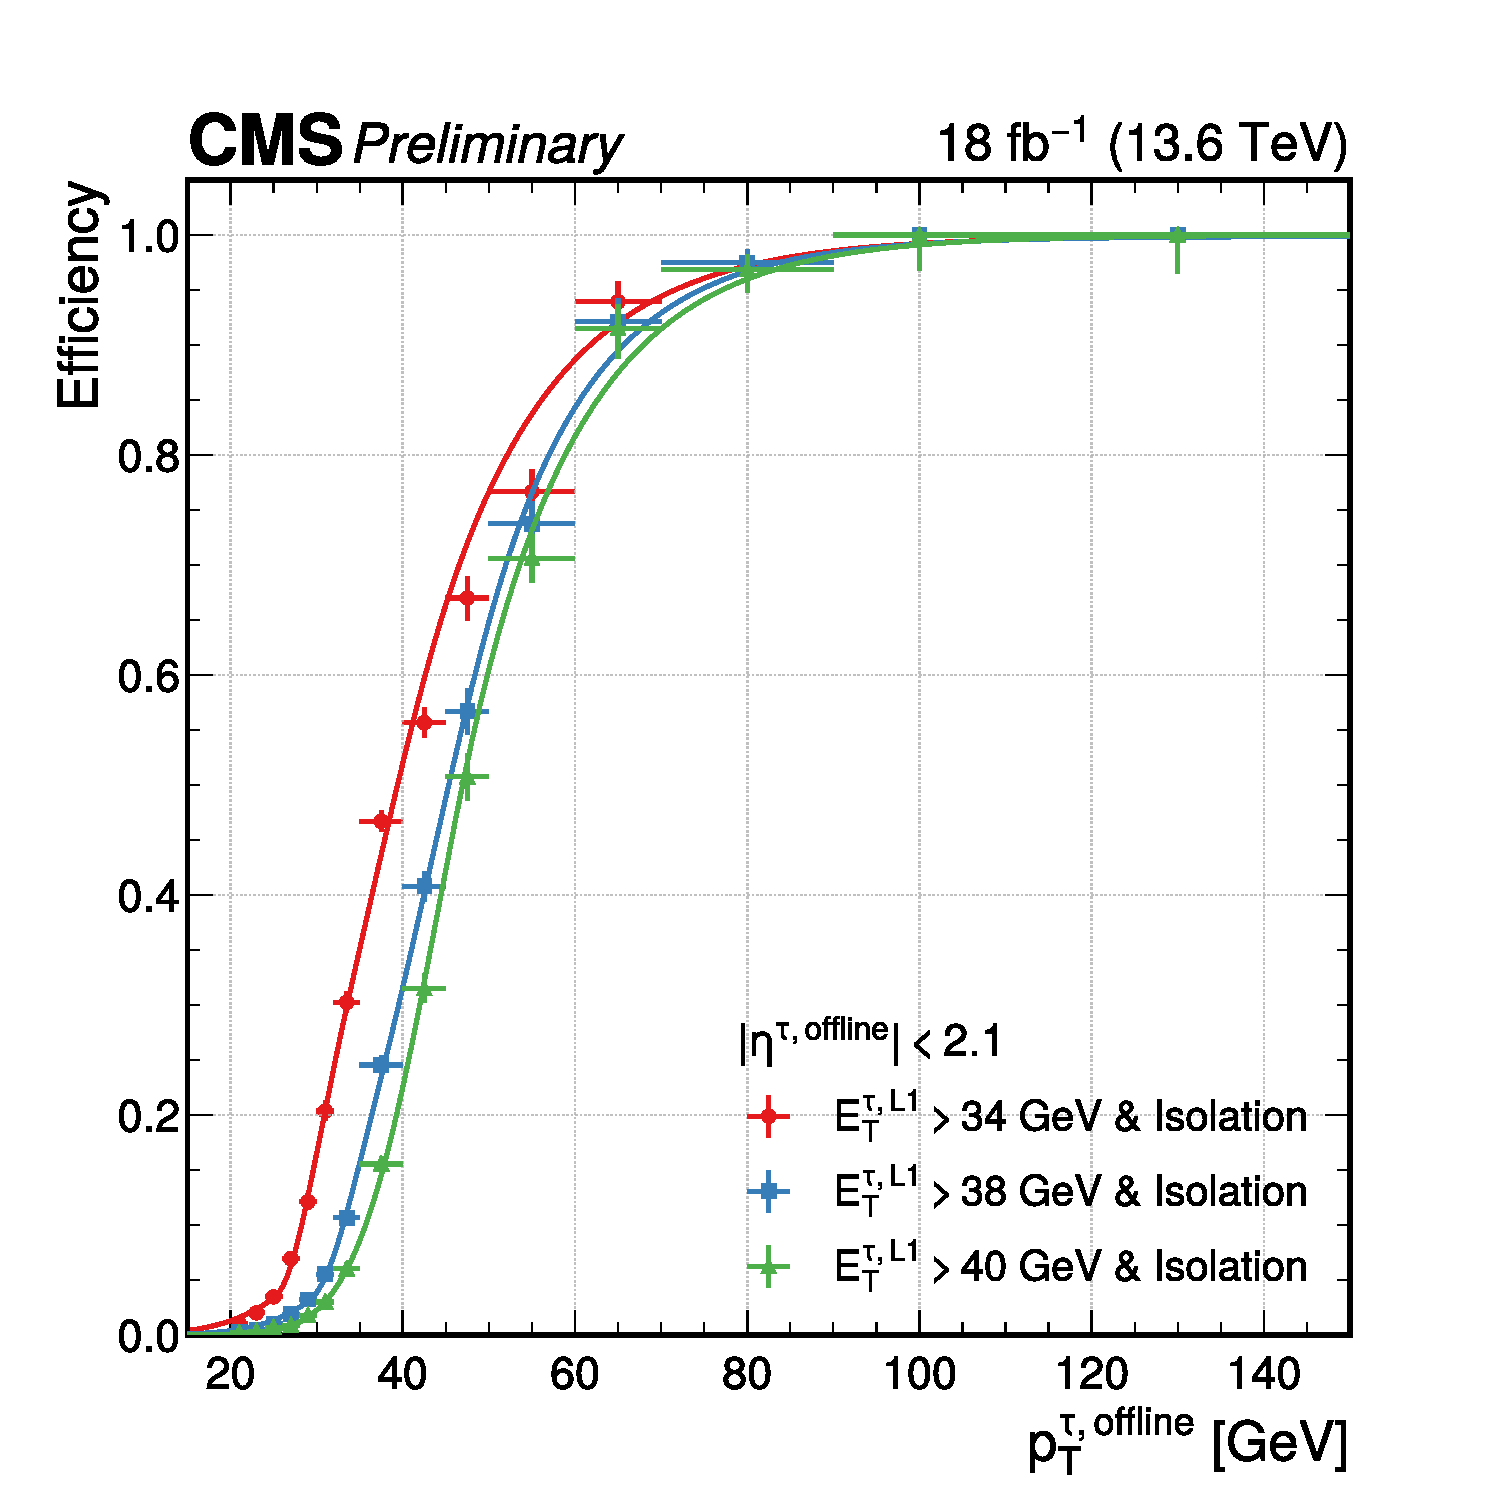
\includegraphics[width=0.4\linewidth]{Figures/L1TP/TauEfficiency.pdf}}
    
    \subfloat[]{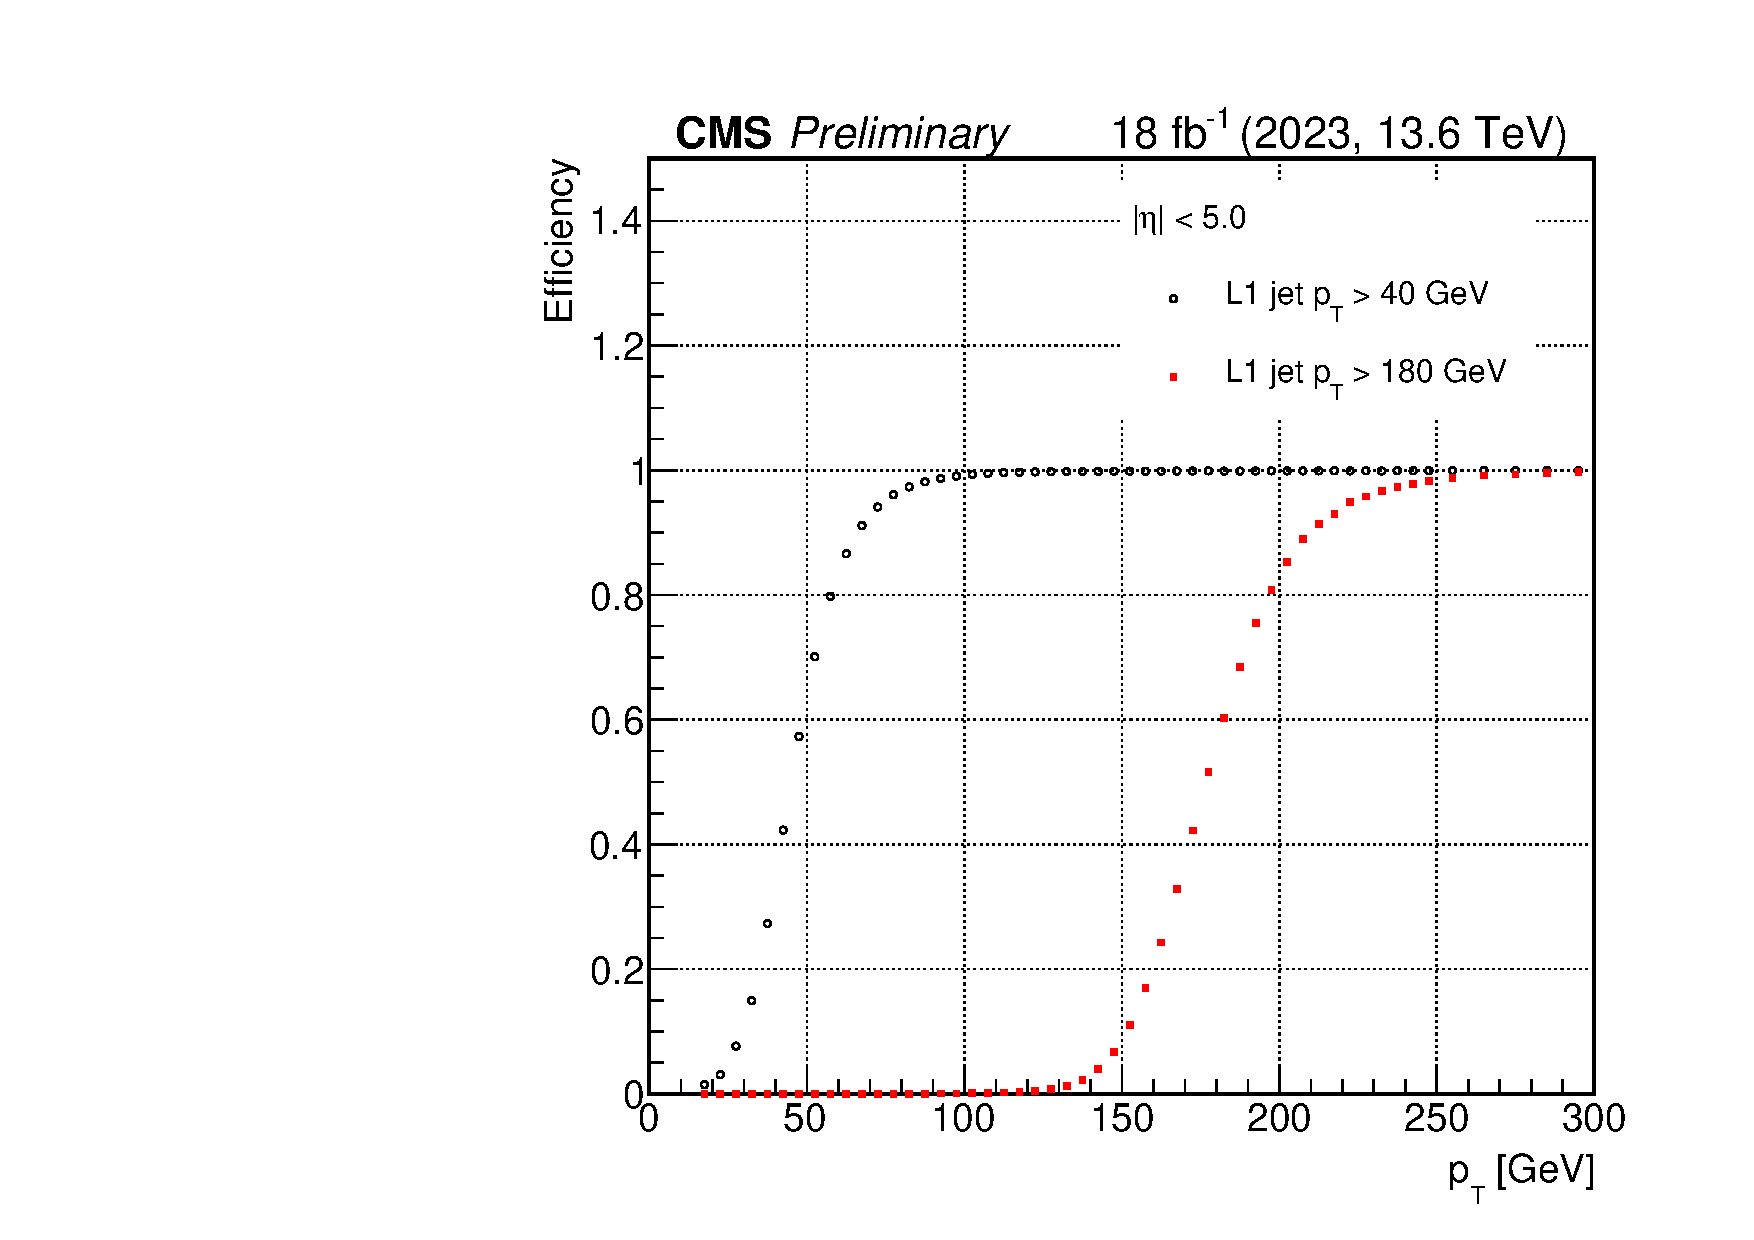
\includegraphics[width=0.4\linewidth]{Figures/L1TP/JetEfficiency.pdf}}
    \subfloat[]{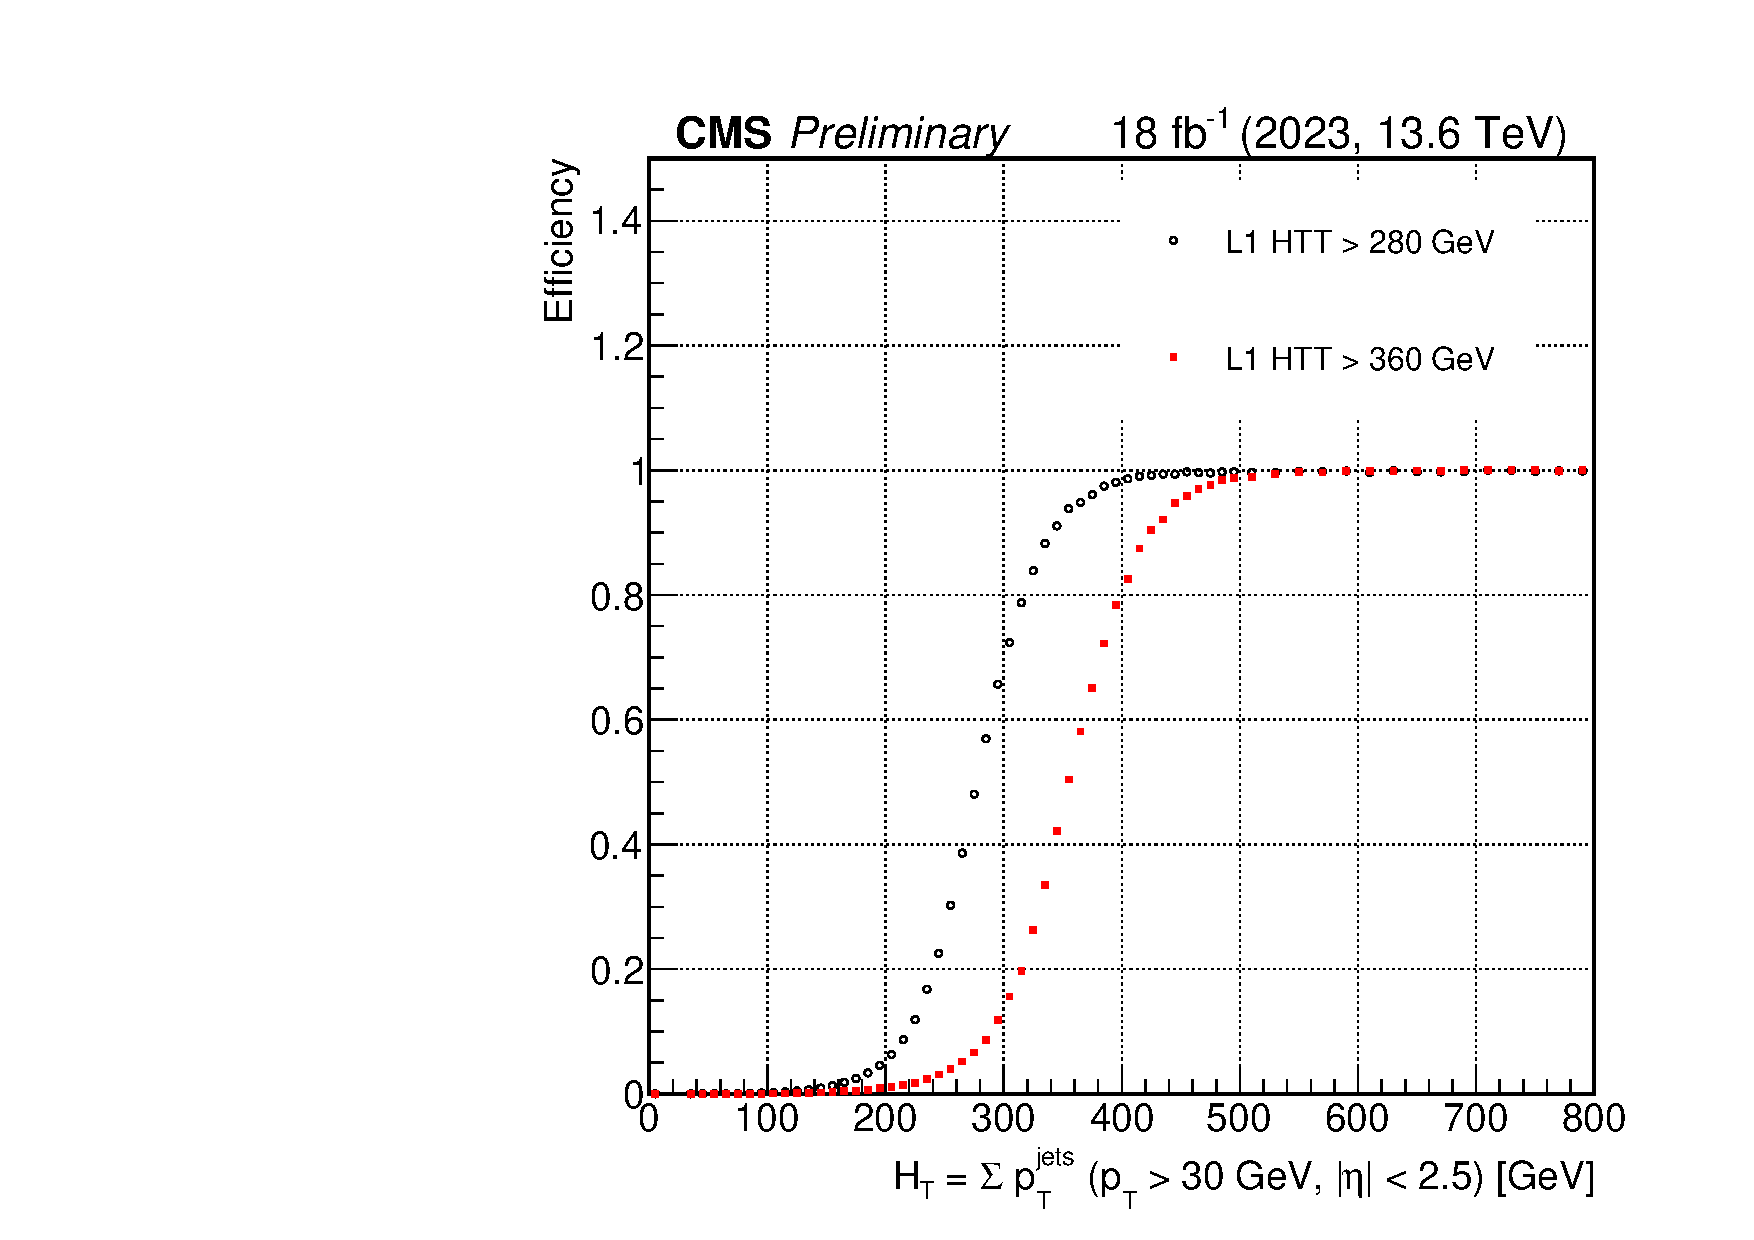
\includegraphics[width=0.4\linewidth]{Figures/L1TP/HTTEfficiency.pdf}}
    \caption{Level-1 performance of L1 calorimeter trigger objects: $e/\gamma$ (a), $\tau_h$ (b), jet (c), and $H_T$ (d). The efficiency turn-on curves are reported for different L1 $p_T$ thresholds.}
    \label{fig:L1Efficiency}
\end{figure}

\bigbreak

The performance of the L1 calorimeter trigger in finding the objects candidate and computing their energy is summarised in Figure~\ref{fig:L1Efficiency}, in terms of efficiency turn-on curves.
The reader will understand, at this point, the considerable importance of Layer-1 calibration in building the L1 calorimeter trigger candidates. 
Given the stacked architecture of Layer-1 and Layer-2, where the latter is fully dependent of the former's output, a better calibration of the TPs at Layer-1 can be crucial in improving the Layer-2 performance.

\section{The current Layer-1 calibration method}
\label{sec:The current Layer-1 calibration}

A first method to extract Layer-1 calibration factors was developed at the beginning of Run~II. 
The approach relies on the extraction of firmware-compatible calibration factors to be applied to the ECAL and HCAL TPs arriving in the Layer-1 calorimeter trigger from the ECAL and HCAL read-out electronics.
The Layer-1 firmware supports a single calibration constant to be applied to each TP, depending on its $i\eta$ position and recorded raw energy.
In this method, the calibration factors are derived in exclusive regions of energy deposit and $i\eta$ position, by comparing the Layer-1 TT response from MC samples to the energy of generated objects~\cite{Sirunyan_2020}.

The ECAL TPs calibration factors are based on MC simulated events of single photon production in the ideal environment of no pile-up, with a flatten transverse momentum spectrum for the photon $p_T \in [0,200]$~GeV, and flatten $\eta$ distribution.
For each event, the generated photons are matched to the corresponding TP, based on the ($\eta$, $\phi$) position, which will be considered as the seed. The $e/\gamma$ candidate is approximated as the $3\times3$ cluster centered around the seed. 
Only clusters containing at least 90\% of the total energy in the central tower are considered for the calibration procedure.
The energy binning is defined according to the energy of the central TP, with a pre-defined binning $E_T\in[0,3,6,9,12,15,20,25,30,35,40,45,55,70,127.5]$~GeV.
The clusters are further divided into 28 bins according to the absolute $i\eta$ position of the central TP, i.e. $|i\eta|\leq28$.
In each ($E_T$, $i\eta$) bin, the differential distribution of the uncalibrated Layer-1 response, defined as the ratio between the generated photon transverse momentum and the $3\time3$ cluster energy deposit $p_T^{\gamma}/E_T^{3\times3}$, is interpolated with a Landau distribution convoluted with a Gaussian distribution.

The HCAL TPs calibration factors are obtained following the same procedure detailed above the ECAL, using a MC sample of double charged pion production in the ideal environment of no pile-up; the pions are characterised by a flatten transverse momentum spectrum $p_T\in[0,200]$~GeV and flatten $\eta$ distribution.
Since objects tend to deposit energy in ECAL before reaching HCAL, the HCAL calibration factors are derived considering ECAL TPs in their derivation, and applying the previously extracted ECAL Layer-1 calibration.
For each event, the generated pions are matched to the corresponding TP, based on the ($\eta$, $\phi$) position, and a window of $5\times5$ in ECAL and HCAL centered around the seeding TP is considered as the jet cluster candidate.
It should be noted that in this method the jet cluster size is significantly reduced with respect to the $9\times9$ chunky donut actually used in the Layer-2 algorithm.
Only clusters containing at least 20\% of the total energy in the central tower are considered for the calibration procedure.
The events are binned according to the energy of the central TP, with the same pre-defined binning as ECAL, and to its absolute $i\eta$ position, i.e. $|i\eta|\leq41 \setminus \{29\}$.
For the HF calibration factors, the ECAL contribution is not considered, as the ECAL detector is not present in that pseudorapidity region.
In both cases, saturated towers with energy $E_T=127.5$~GeV are ignored by the calibration procedure. 

The calibration factors are originally designed to be extracted by the mean of the fitted distribution; however, given the presence of large tails towards higher energies, the method has been upgraded in 2018 to use the mode, i.e. the value that appears most frequently in the distribution.
An example for the interpolation of the response distributions is reported in Figure~\ref{fig:OldL1Fit}, for ECAL $E_T \in [0,3]$~GeV and $i\eta=1$~(a), and for HF $E_T \in [0,3]$~GeV and $i\eta=31$~(b).

The extracted calibration constants are stored in three firmware-compatible Look-Up-Tables (LUT), for ECAL, HCAL, and HF respectively. In total, for 13 energy bins and 40 pseudorapidity rings, 520 scale factors are defined, and encoded into 10-bit digital variables.
The resulting values are summarised in Figure~\ref{fig:L1OldSF} for ECAL and HCAL TPs, as a function of $i\eta$ and $E_T$.
The increase of the calibration factors with $\eta$ reflects the profile of the detector material in front of the calorimeters. The choice of the binning respects the hardware limitation and takes into account the dependency of the resolution in $E_T$.

\begin{figure}
    \centering
    \subfloat[]{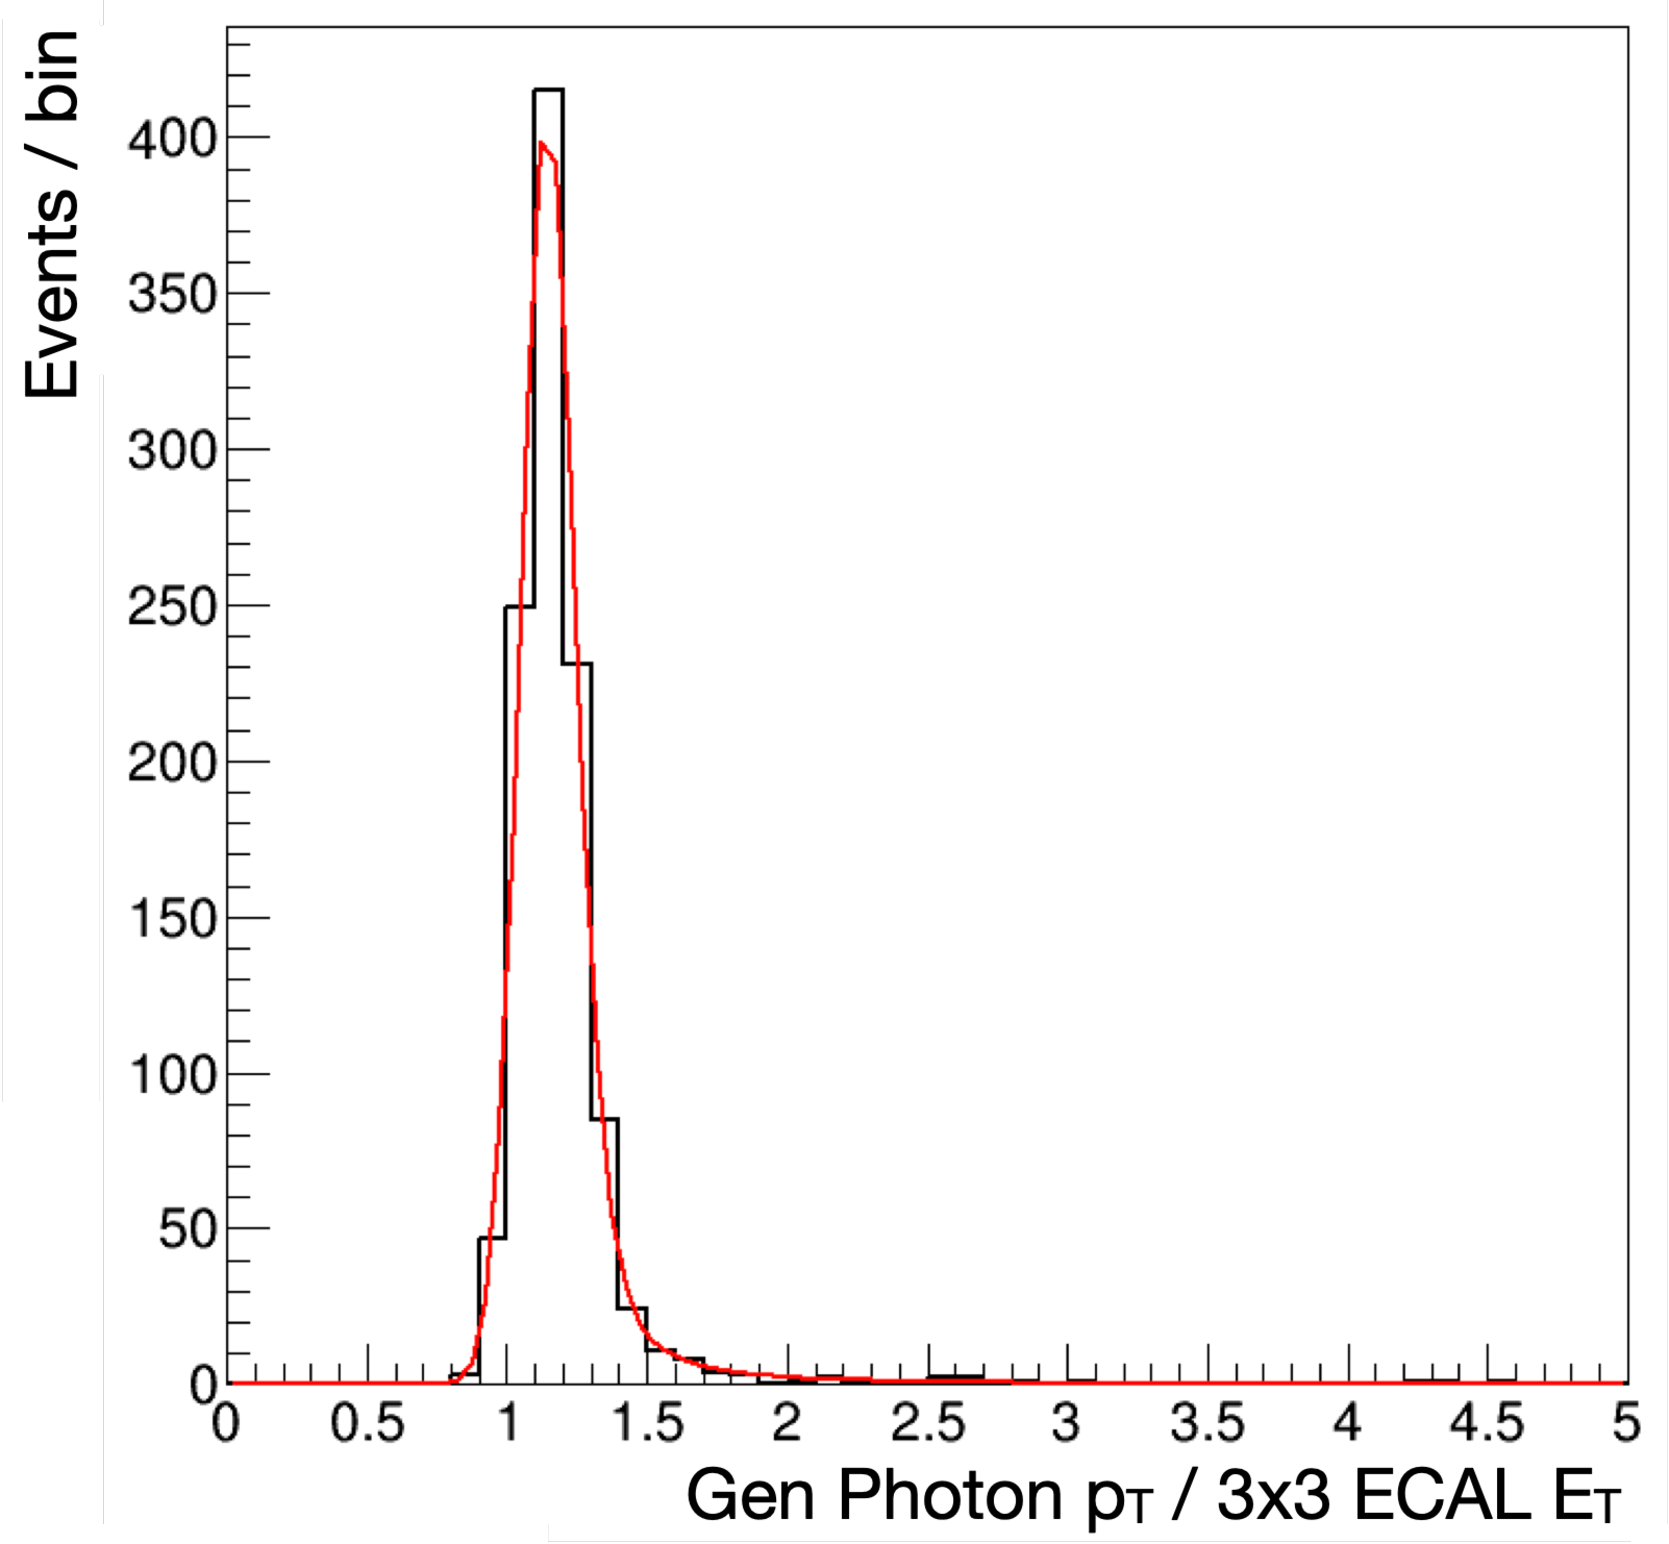
\includegraphics[width=0.4\linewidth]{Figures/L1TP/OldL1ECAL.pdf}}
    \hspace{0.7cm}
    \subfloat[]{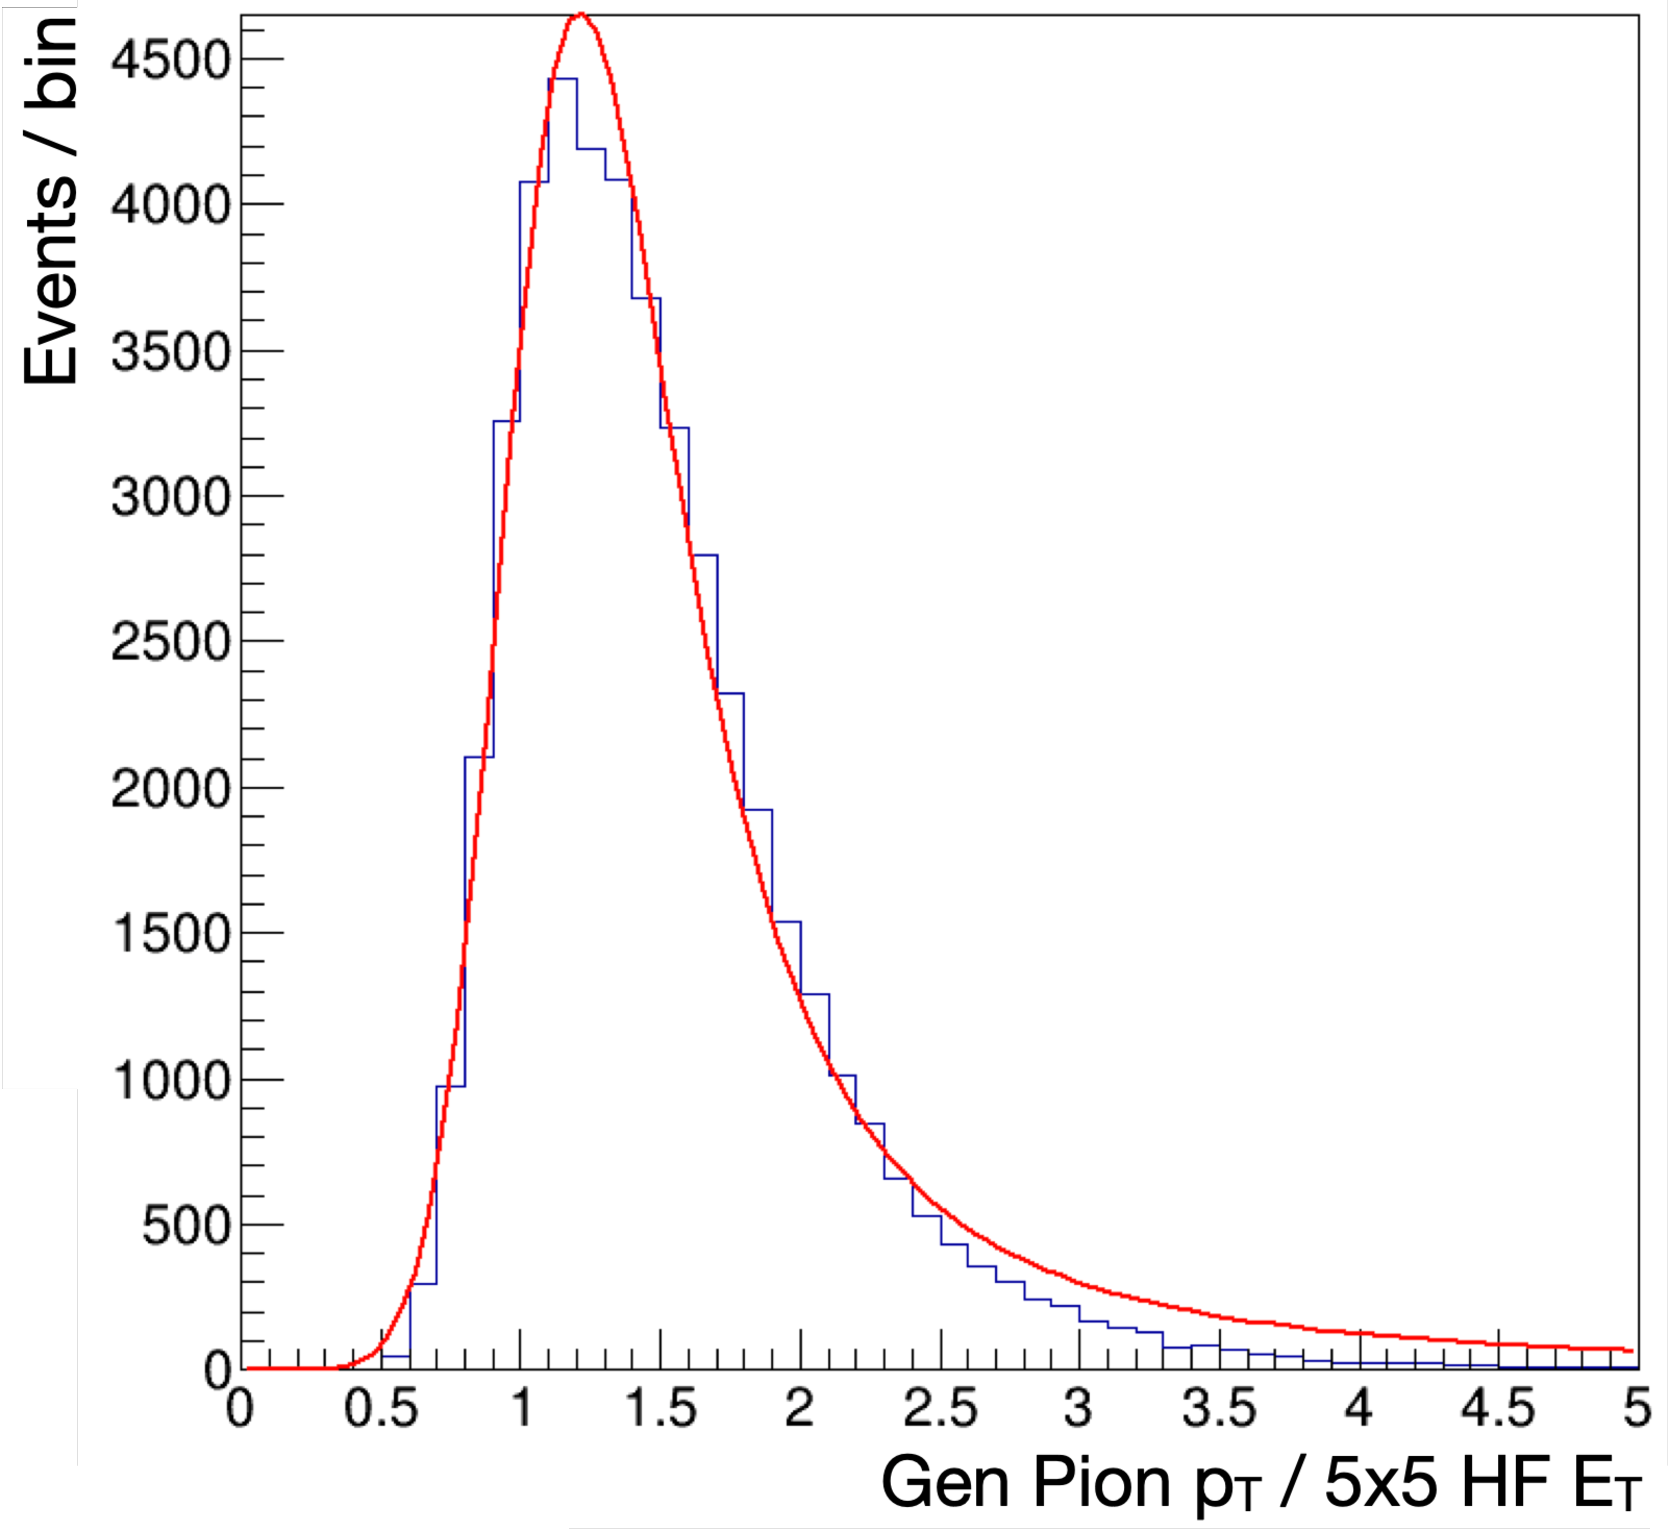
\includegraphics[width=0.4\linewidth]{Figures/L1TP/OldL1HF.pdf}}
    \caption{Distribution of the Layer-1 energy response fitted with a Landau distribution function convoluted with a Gaussian. For ECAL, the response is defined as the ratio between the generated photon transverse momentum and the $3\time3$ $e/\gamma$ cluster energy deposit for $E_T \in [0,3]$~GeV and $i\eta=1$~(a). For HCAL and HF, the response is defined as the ratio between the generated pion transverse momentum and the $5\time5$ jet cluster energy deposit for $E_T \in [0,3]$~GeV and $i\eta=31$~(b).}
    \label{fig:OldL1Fit}
\end{figure}

\begin{figure}
    \centering
    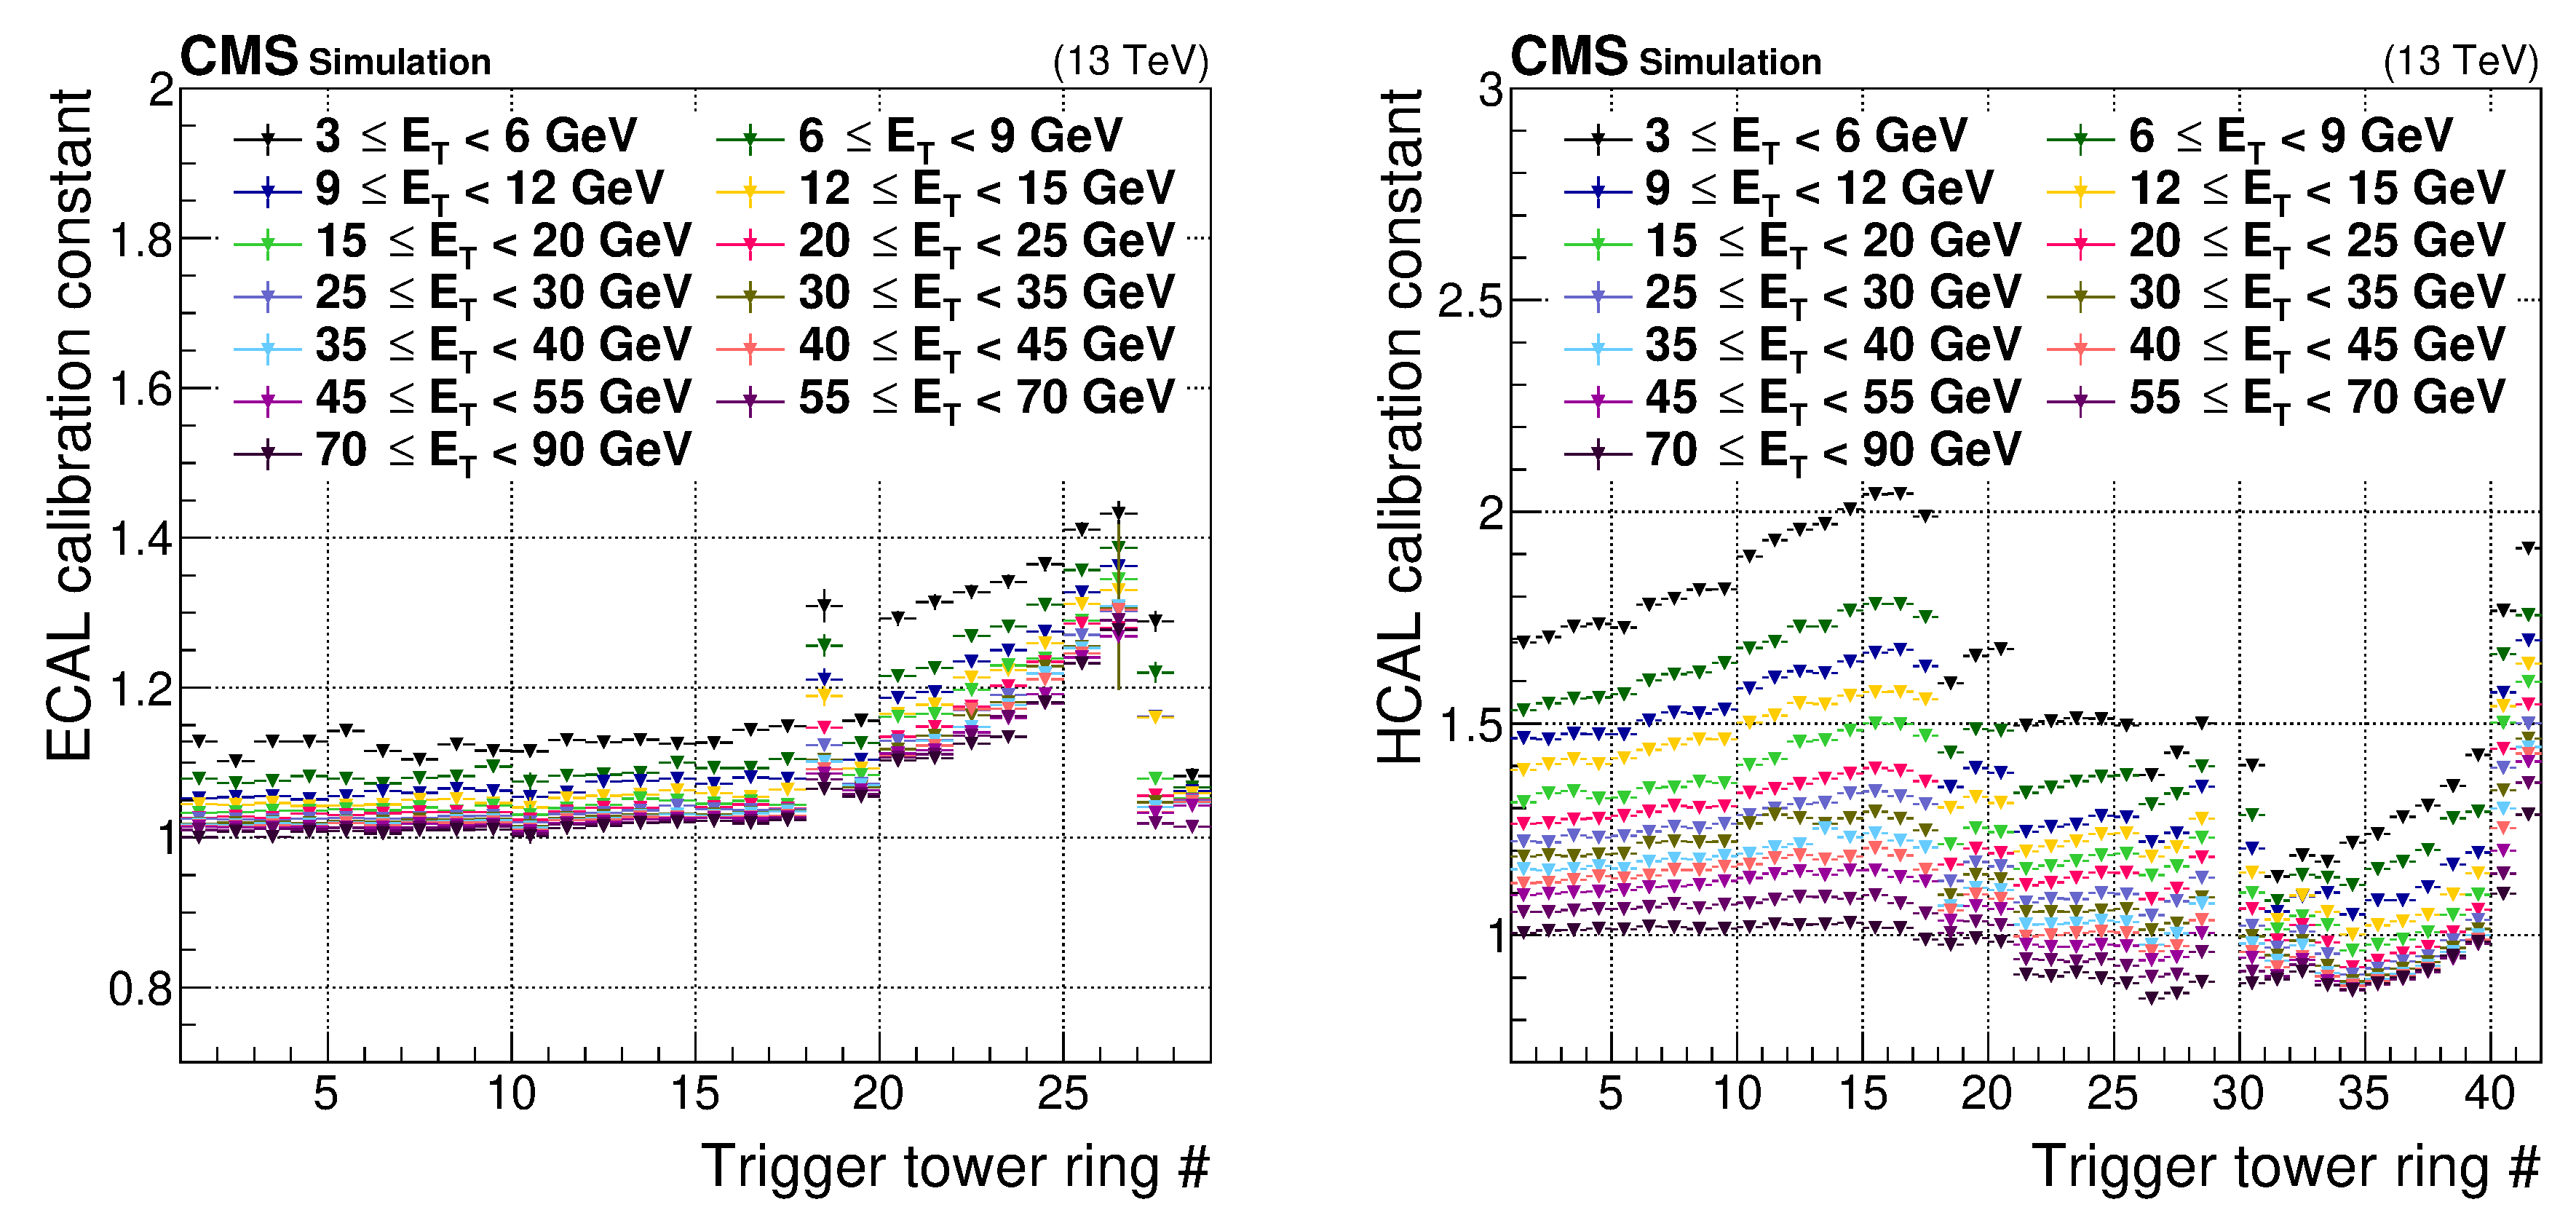
\includegraphics[width=0.9\linewidth]{Figures/L1TP/L1OldSF.pdf}
    \caption{Layer-1 energy scale factors for ECAL (left) and HCAL (right), shown for each constant-$|\eta|$ ring of Trigger Primitives (TP). As specified in the legend, the color of each point corresponds to a range of uncalibrated TP transverse energy values received by the Layer-1 calorimeter trigger. Because of the HCAL geometry, the signals from TPs ring 29 are divided between rings 28 and 30, and no scale factors are applied.}
    \label{fig:L1OldSF}
\end{figure}

\bigbreak

The current method for the extraction of Layer-1 calibration factors has achieved good results throughout Run-II, but suffers from inherent criticality. 
The method is based on the use of MC simulated samples, with particular conditions in terms of flatten energy and $\eta$ distributions, and is affected by its finite statistical power. 
In order to ensure comparable and sufficient statistics in all bins, the approach requires the definition of a small number of coarse energy bins, while the firmware would allow for a finer binning up to one calibration factor every energy digit, i.e. 0.5~GeV.
Moreover, MC samples are based on the simulation of the detector response to generated particles and the simulation of the response in low energy TPs have proven to be not entirely reliable and highly dependent on the continuously varying detector conditions.
Another critical point comes from the definition of the $e/\gamma$ and jet cluster candidates, which does not follow the same algorithm employed in Layer-2; in particular, the HCAL shower can spread beyond the $5\times5$ extension of the cluster.
In addition, once the cluster of multiple TPs has been defined, the calibration factor is only extracted for the central TP through a linear regression. This approach completely ignores any possible dependency on the energy distribution within the cluster or any correlation between different TPs.

These points have become particularly evident at the start of the Run~III data-taking. 
The optimization of ECAL, HCAL, and HF calibrations was performed, but in the case of HCAL and HF, the new correction factors did not pass the necessary validation and closure tests. 
For this reason, for the Run~III data-taking, the choice was made to set HCAL and HF Layer-1 calibration factors to unity, thus removing the needed calibration.

\section{The new Layer-1 calibration method}

A novel ML technique for the detector calibration has been developed for the extraction of Layer-1 calibration factors, aiming to address some of the critical limitations related to the current calibration technique described in the previous section.
This application provides a first proof of concept for the novel ML-based calibration method and offers insights into its potential future applications beyond the L1 Trigger context.

\bigbreak

The primary improvement introduced by the new method stems from the use of ML algorithms to derive calibration constants. Unlike traditional techniques that require the definition of a simplified parametric function to describe the energy response, the ML approach can handle complex, non-linear relationships, which are typically difficult to capture with conventional regression methods. 
ML models can learn from large amount of data simultaneously and interpolate the detector response even for objects that were not included in the training dataset.
Moreover, the capability of ML methods to incorporate multiple input variables allows for a faster extrapolation of the calibration constants, without necessitating finite, coarse energy bins. However, in this specific application, the calibration factors are constrained by firmware compatibility, necessitating a minimum energy bin size of $\Delta E_T\geq0.5$~GeV.

The second improvement comes from a redefinition of the clusters defining the $e/\gamma$ and jet candidates. 
According to the Layer-2 conventions for the hadronic jet candidates, the L1 cluster is defined, both for $e/\gamma$ and jet objects, as the $9\times9$ matrix of TTs composing the \textit{chunky donut} (CD). This choice ensures maximal containment of the hadronic shower, and minimal energy loss. This inclusive definition of the L1 cluster has revealed itself as a convenient approach for the calibration of jets, whilst the $e/\gamma$ cluster, initially defined as the same $9\times9$ TTs CD shape, has been subsequently revised to a smaller shape, in order to reduce the contamination from pile-up. 
In the new method, no requirements are applied to the energy deposit in the central TP, allowing for different candidate shapes to enter the calibration process, expanding the effectiveness of the calibration to account for a wider range of possible shapes.

Finally, the method described in this Chapter is based on the possibility of extracting the calibration factors using either MC simulated events or data. In the first case, the calibration method benefits from a better definition of the true object energy at generator level, and from the simulation of the ideal environment of no pile-up, hardly achievable during ordinary data taking conditions. In the latter, the use of data presents more arduous conditions due to the inevitable contribution of pile-up, however it provides the most reliable representation of the latest detector response, with continuously increasing training datasets as more data becomes available.
The design and optimisation of the method is performed based on data collected by the CMS Experiment, with two separate samples for the derivation of the ECAL and HCAL/HF calibration constants.
For the derivation of the ECAL calibration factor, the \texttt{EGamma} dataset is used, which is composed of events triggered by HLT paths requiring the presence of electron or photon candidates. For the derivation of the HCAL/HF calibration, the \texttt{JetMET} dataset is used, which is recorded by requiring the presence of jet or missing transverse energy candidates.

% \bigbreak

% The first implementation of the new Layer-1 calibration method was based on a Neural Network (NN) approach~\cite{Motta:2881939}, which I contributed in developing and optimising. This initial attempt is discussed in Section~\ref{sec:The Neural Network approach}, however it was found to have intrinsic limitations for the specific application of the calibration to the Layer-1 context. 
% As part of this Thesis work, I have converted the NN method into a new algorithm based on differentiable programming, allowing for streamlined parameter optimisation and customisation of the Layer-1 calibration constants for a better compatibility with the Layer-2 requirements.

% The Trigger Primitives that used to build the Level-1 Trigger calorimeter objects (electron, photon, tau leptons, jets, etc.) are calibrated using the method described in Ref. \cite{CMS:2020cmk}. It consists in deriving calibration factors for the ECAL and Hadronic Calorimeter (HCAL) from single-photon (single-pions)
% simulations. The calibration factors are extracted, in bins of $\eta$ and transverse energy, from the distribution of the calorimeter response, i.e. the ratio of the true particle energy (a photon or a pion) to the energy of a group of 3 (9) Trigger Primitives.\\

\section{The Neural Network approach}
\label{sec:The Neural Network approach}

The first implementation of the new method for the extraction of Layer-1 calibration factors is based on a NN approach, which I contributed in developing and optimising.
The idea behind this first implementation is to exploit innovative and widely employed software techniques to bypass the drawbacks of the standard linear regression method, taking advantage of the ability of NNs to model complex, non-linear relationships and to efficiently handle large datasets.
Moreover, the NN approach entirely removes the need for arbitrary choice of energy binning to perform fits and can learn about possible correlations between the different TTs composing the L1 candidate.

The input to the NN is the raw energy deposit $E_T$ and $i\eta$ position of each TT composing the $9\times9$ L1 candidate.
The goal of the NN approach is learning to predict the best calibration factors to be applied to each TT so that the calibrated L1 energy is as close as possible to the reference value, defined as the energy of the reconstructed object:

\begin{equation}
    E_T^{\,L1,\;jet} = \sum_{i\eta,\:i\phi}\left(\;\alpha\,(i\eta,E_{T})\;\cdot\;E_{T}\;\right) 
    \;\longrightarrow\;
    E_T^{\:Reco,\;jet}
\end{equation}
where $E_T^{\,L1,\;jet}$ is the calibrated L1 energy, $\alpha\,(i\eta,E_{T})$ are the calibration factors, depending on the $E_T$ energy deposit and $i\eta$ position of the TT, and $E_T^{\:Reco,\;jet}$ is the energy of the reconstructed object.

\subsection{Basic concepts of Neural Networks}

The main idea behind NNs is reproducing the neuronal organisation found in animal brains through software implementations~\cite{1672070}.
The structural building blocks of NNs are artificial neurons, also known as \textit{perceptrons}, taking as input $n$-dimensional vectors of variables $(x_1,x_2,...,x_n)$. Each variable is multiplied by a different weight $w_i$ and summed together, adding a bias term $b$.
The outcome of the summation is then fed into an activation function $f$, which can be either linear or non-linear, the latter option generally being preferred as the introduction of non-linearity enables the NN to capture arbitrarily complex relationships in data.
Mathematically, each artificial neuron can be represented as a unit performing the following operation:
\begin{equation}
    \hat{y}=f\left( \sum_{i=1}^{n}w_i \cdot x_i + b \right)
\end{equation}
where $\hat{y}$ represents the output of the neuron, and the process of feeding the inputs to a neuron is known as \textit{forward propagation}. A graphical illustration of the neuron can be found in Figure~\ref{fig:Perceptron}.

\begin{figure}
    \centering
    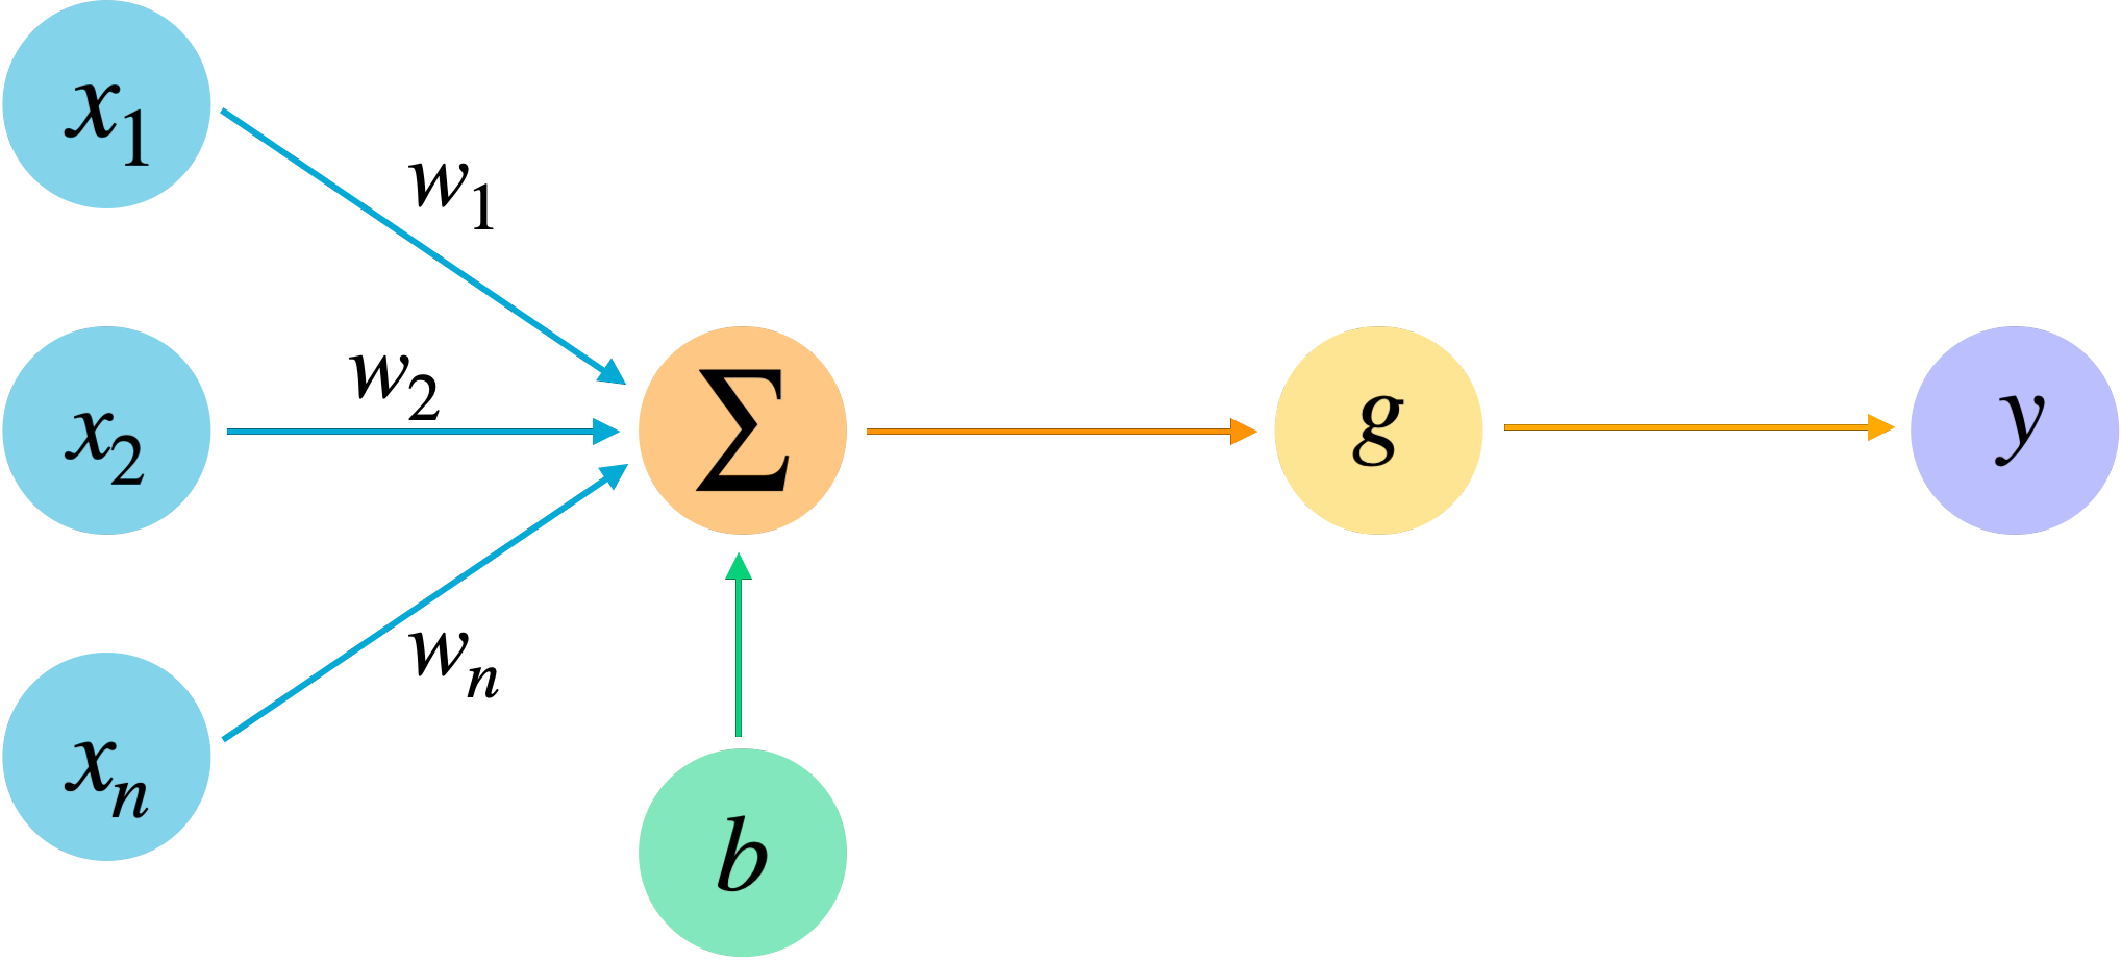
\includegraphics[width=0.6\linewidth]{Figures/L1TP/Perceptron.pdf}
    \caption{Graphic illustration of an artificial neuron. An $n$-dimensional vector of variables is passed as input, and weights are applied to each element. The weighted vector is summed and added to a bias term, the sum is passed to a non-linear activation function $f$, which returns the output $y$.}
    \label{fig:Perceptron}
\end{figure}

In a typical NN architecture, neurons are arranged into layers, and each neuron in a layer receives inputs from the neurons in the preceding layer. 
The structure of the NN is fully defined by the configuration of these layers and the number of neurons in each layer. A typical NN includes an input layer, multiple hidden layers, and an output layer, as illustrated in Figure~\ref{FIXME}.
% The output layer can produce one or multiple output values, depending on the specific problem being addressed. 
At this stage, the NN is simply a sequence of neurons, taking as input a set of variables, and computing mathematical operations to generate the output. The degree of complexity of the NN function is directly related to its architecture: at a first approximation, the number of layers corresponds to the degree of the polynomial functions, while the number of neurons in each layer regulates the monomials of the same degree. 

Once the NN architecture is defined, the goal is to adjust the NN weights in such a way that the prediction for the final output $\hat{y}$ is as close as possible to the truth value. 
In order to quantify the discrepancy between the NN prediction and the real quantities, different metrics can be adopted, generally referred to as \textit{loss functions}:
\begin{equation}
    L(w,b)=\frac{1}{N}\sum_{j=1}^N(y_j-\hat{y}_j)^2
\end{equation}
where $N$ is the number of input samples, $y_i$ is the truth value being learnt, and $\hat{y}_i$ is the predicted NN output.
The minimization of the loss function, also known as \textit{training}, is achieved by feeding the NN with a dataset where the truth value $y_i$ of the target variables are already known.
During the training process, the loss function is derived with respect to the weights, and the trainable parameters are progressively updated in the opposite direction to the gradient, thus guiding the NN weights to values that minimise the loss. The procedure of updating the weights following the loss gradient is usually referred to as \textit{backward propagation}, and can be tuned by a learning rate parameter defining the magnitude of the parameter variation during each training iteration. A small learning rate leads to slow convergence and risks getting the NN trapped in local minima, whereas a large learning rate can cause the process to overshoot the optimal weights, resulting in instability and divergence.

After initialising the weights to random values, the process of training a NN model is constituted by an iterative repetition of the following steps, until convergence:
\begin{itemize}
    \item Evaluate the loss function with the current set of weights, $W$ (\textit{forward propagation});
    \item Compute the gradient of the loss function with respect to the set of weights, $\partial L/\partial W$;
    \item Update the weights in the opposite direction to the gradient, with a step proportional to the learning rate, $W = W - (\partial L/\partial W \times LR)$ (\textit{backward propagation}).
\end{itemize}
A schematic overview of a typical NN architecture and its training process is reported in Figure~\ref{fig:Architecture}.

\begin{figure}
    \centering
    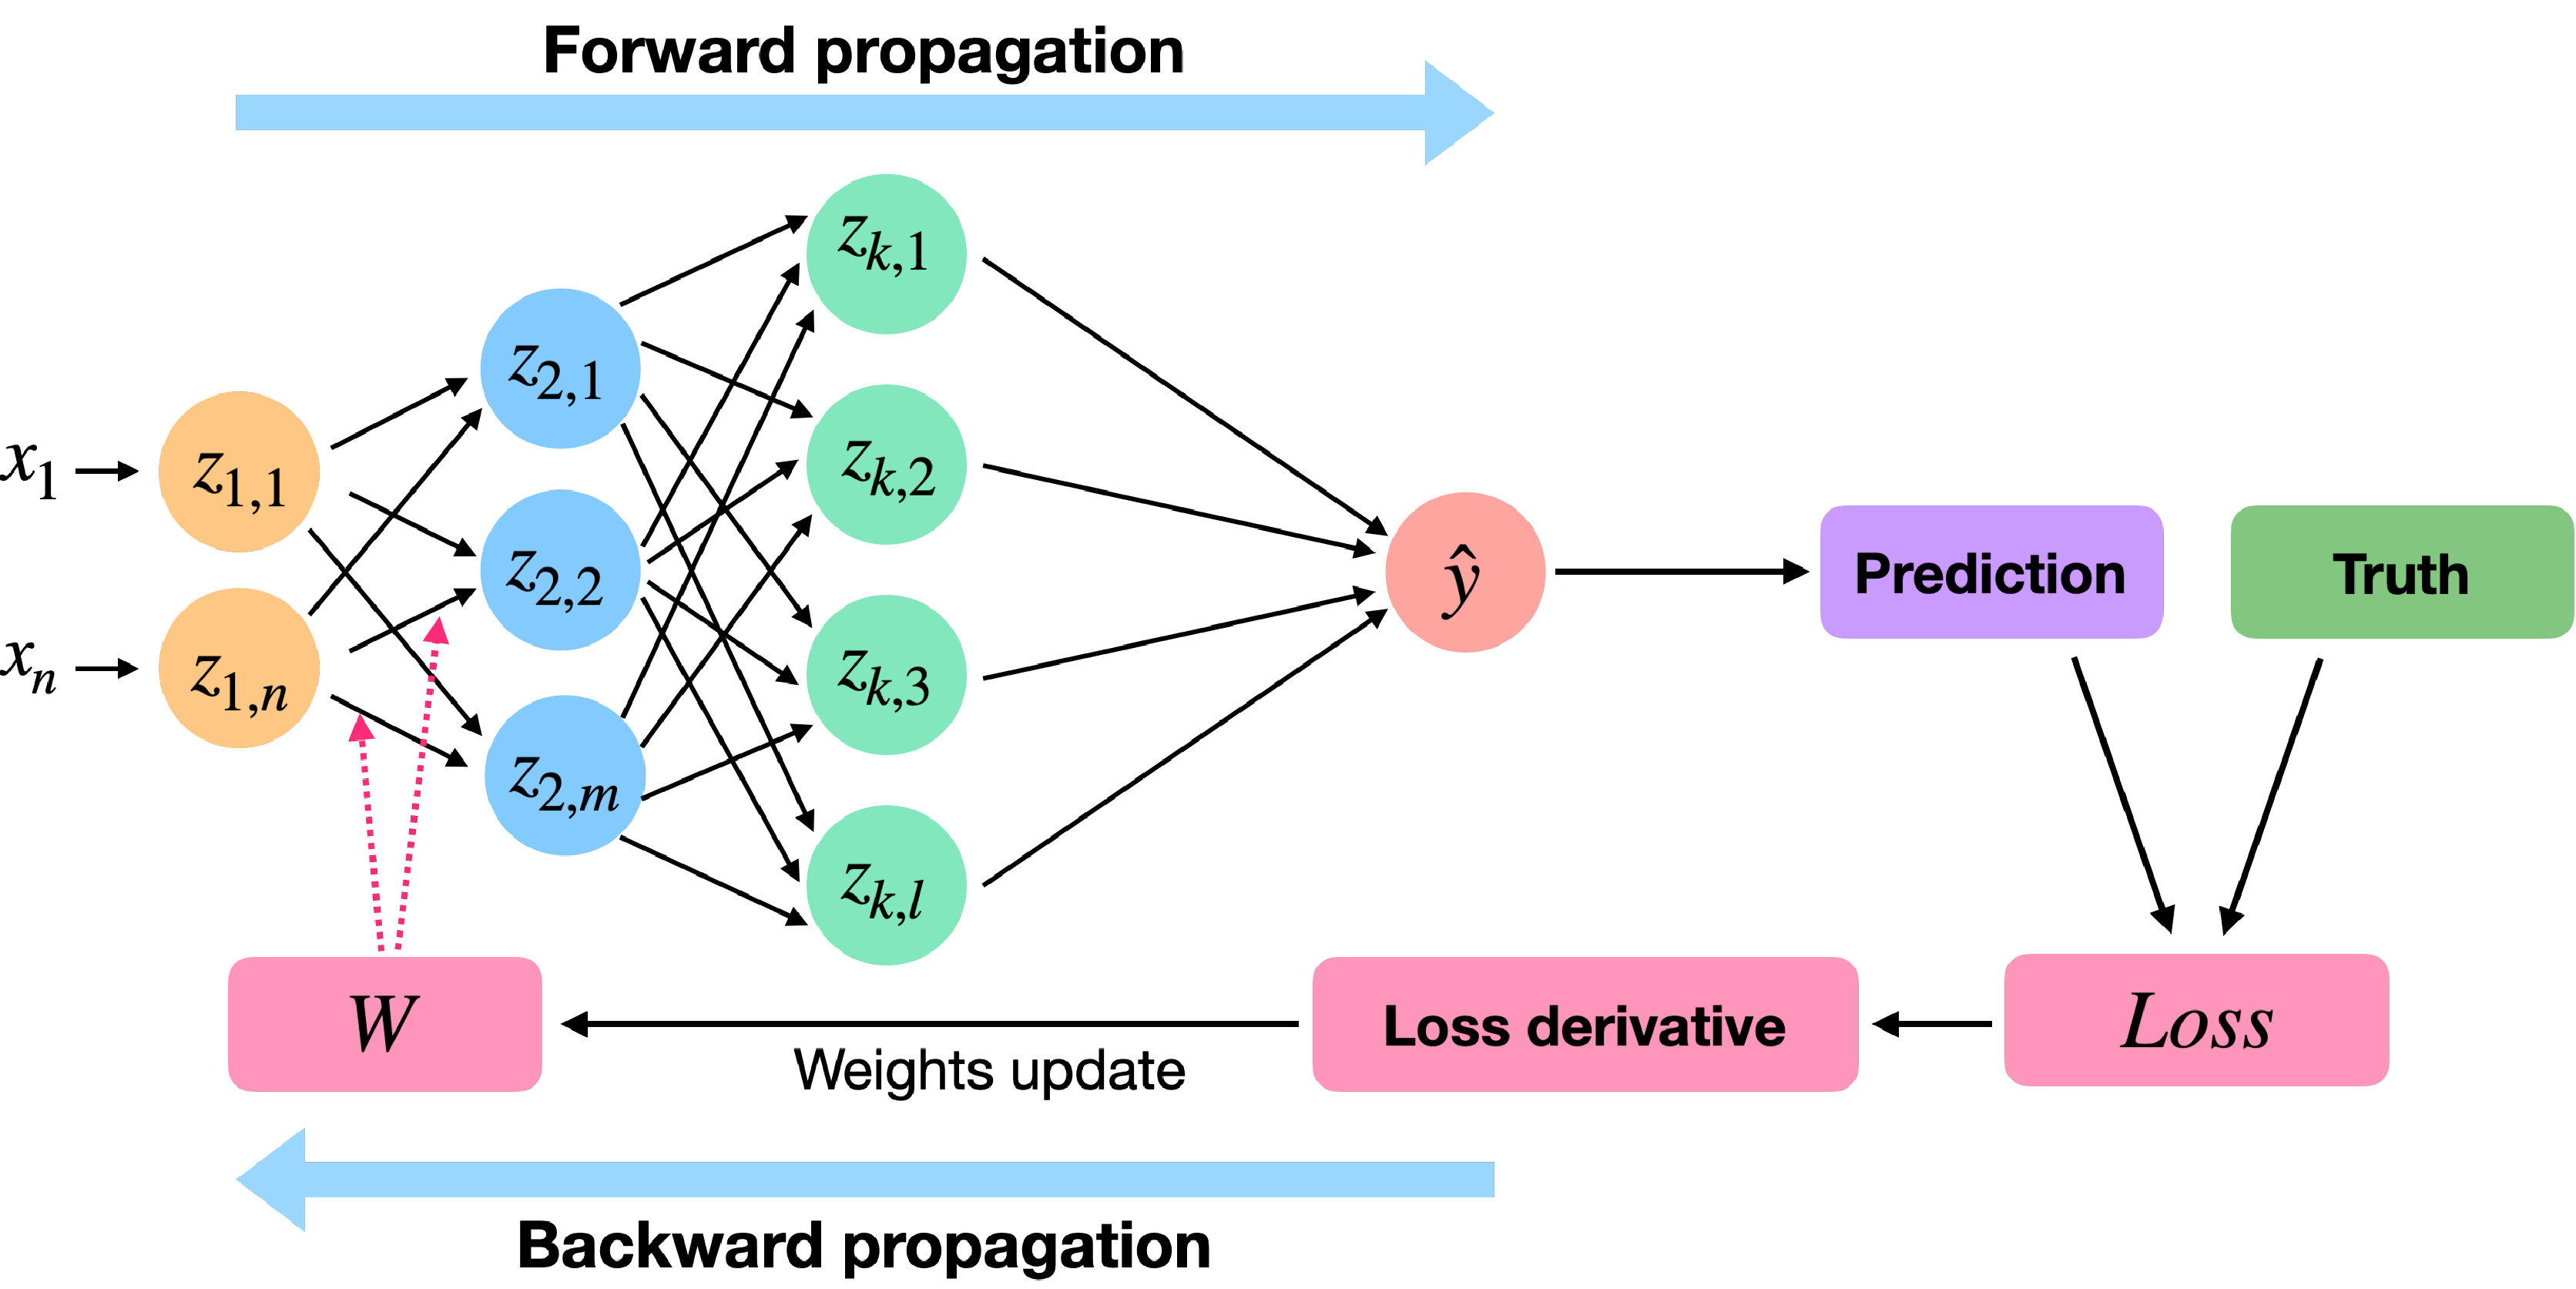
\includegraphics[width=0.8\linewidth]{Figures/L1TP/Architecture.pdf}
    \caption{Schematic representation of a typical Neural Network (NN) architecture, alongside its basic training steps. The input data is fed to the NN, which processes it in the forward propagation to give a prediction; the loss function is computed, encoding the discrepancy between prediction and truth values; in the backward propagation, the loss is derived and the trainable parameters are updated according to an optimizer that minimizes the loss function.}
    \label{fig:Architecture}
\end{figure}

% \subsection{Input definition}
% In the new ML-based method, the L1 objects are defined as a $9\times9$ matrix of TTs, and the Layer-1 raw energy of each candidate is defined as the sum of the $iE_T$ energy deposit in the 

\subsection{The algorithm architecture and training} 

The NN designed for the Layer-1 TTs calibration is based on a custom architecture, in order to handle the input features coming from the position and raw energy of the TTs composing the $9\times9$ CD, and extract the predicted calibrated energy of the L1 candidate.

% architecture
A schematics of the NN architecture is reported in Figure~\ref{fig:TTP}.
The basic building block of the NN architecture is the Trigger Tower Predictor (TTP), a stand-alone network, which takes as input the energy deposit and $i\eta$ position of a single TT and extracts the predicted calibrated TT energy.
The TTP is structured as a fully connected layer with 84 neurons, a hidden layer with 256 neurons, and one single-neuron output layer. All neurons make use of the Rectified Linear Unit (ReLU)~\cite{4082265} activation function, and the bias parameter is inhibited in order to avoid propagating the information of empty TTs.
In order to simulate the Layer-1 firmware algorithm, which is based on the transmission of 8-bit words with discrete values for TT the energy deposit, a custom layer is applied to the output of the TTP, flooring the output of the previous layer in units of $iET$ (i.e. 0.5~GeV precision).
The TTP is cloned 81 times, to reproduce the $9\times9$ array of TTs, with each clone sharing the same trainable parameters.
The outputs of the 81 TTP clones are then summed together in a non-trainable \textit{summation layer}, to obtain the predicted calibrated L1 candidate energy.

\bigbreak

\begin{figure}
    \centering
    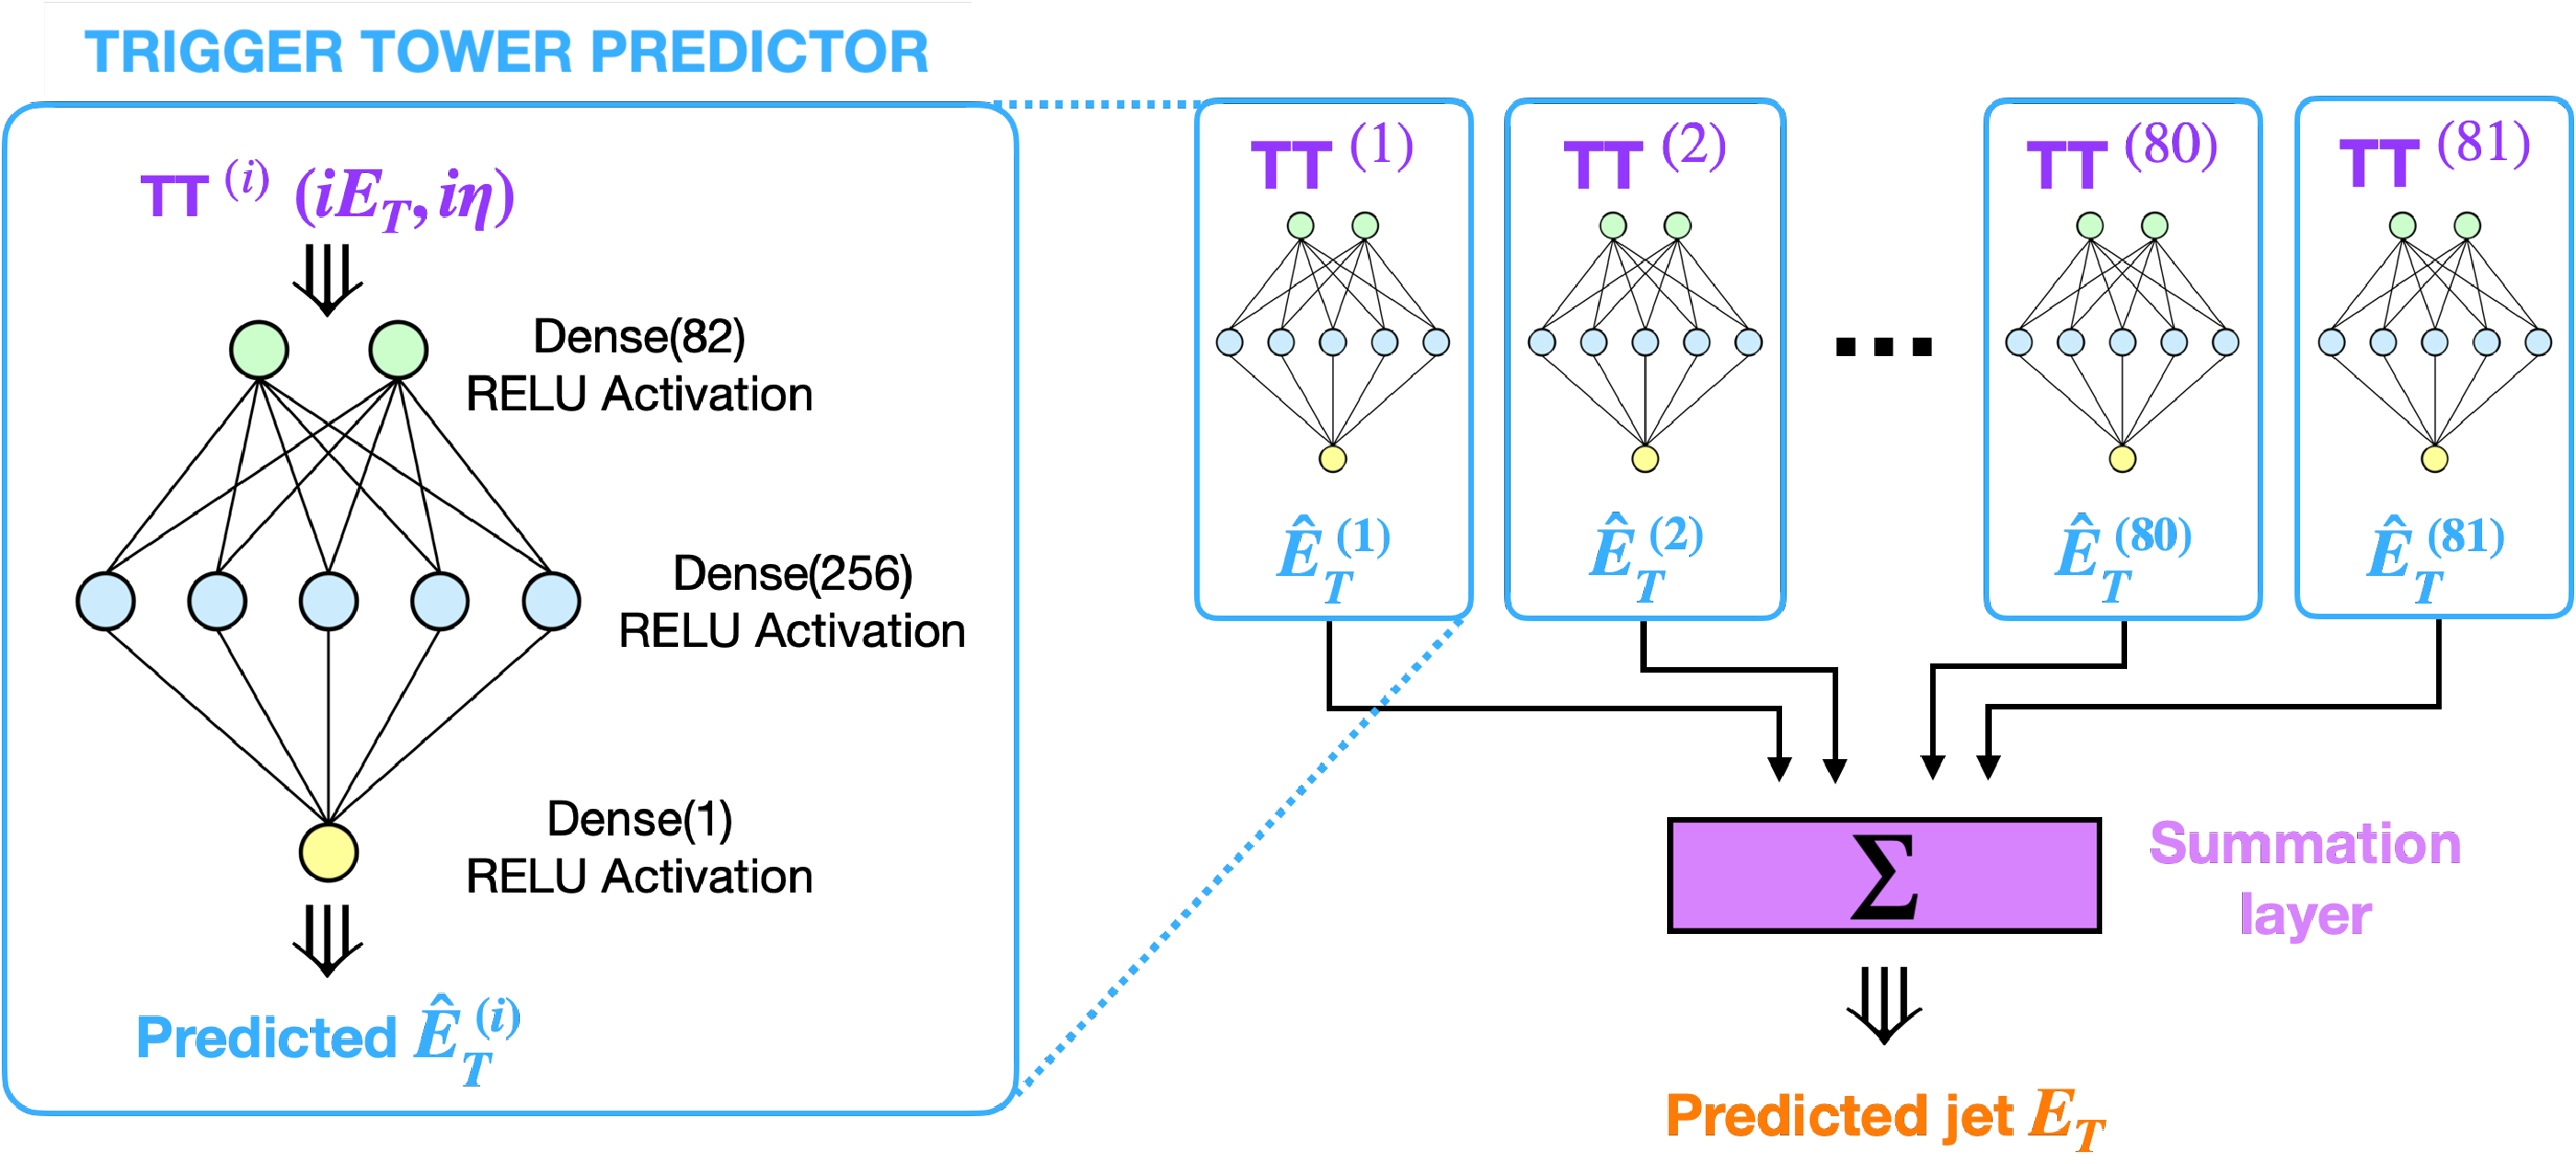
\includegraphics[width=0.8\linewidth]{Figures/L1TP/TTP.pdf}
    \caption{Schematic view of the NN architecture. The basic component is the Trigger Tower Predictor (TTP), a stand-alone NN, which takes as input the energy deposit and $i\eta$ position of a single TT and extracts the predicted calibrated TT energy. The TTP is cloned 81 times, and the outputs are summed together in the summation layer, to extract the predicted calibrated L1 candidate energy.}
    \label{fig:TTP}
\end{figure}

% Training
Once the NN architecture has been defined, the training is performed by minimising a custom loss function, containing three different terms:
\begin{itemize}
    \item \textit{Regression term}: it evaluates the distance between the predicted L1 calibrated energy, at the output from the summation layer, and the target offline energy of the matched object, by using the Mean Absolute Percentage Error (MAPE) function.
    \item \textit{Regularisation term}: it is computed as the squared sum of all the network’s weights and maintains the trainable parameters small, in order to avoid neuron subset over-training.
    \item \textit{Rate term}: it is a penalty term based on the evaluation of the L1 rate proxy, with the effect of maintaining the estimated L1 rate close to the current level.
\end{itemize}
Each term is regulated by a multiplication factor, considered as a NN \textit{hyper-parameter}, that can be varied to adjust the relative importance of each term to optimise the NN performance. The loss function is mathematically expressed as:
\begin{equation}
L = 
A\cdot\left|\frac{E_T^{L1,\;jet} - E_T^{Reco,\;jet}}{E_T^{Reco,\;jet}}\right|
\;+\;
B\cdot\sum_iw_i^2
\;+\;
C\cdot\cosh\left(D\cdot\frac{R_{proxy} - R_{target}}{R_{target}}\:\right)
\end{equation}
where $E_T^{\:L1,\;jet}$ and $E_T^{\:Reco,\;jet}$ are the energy of the calibrated L1 candidate and of the offline object respectively, $w_i$ is the NN trainable parameter, and $R_{target}$ and $R_{proxy}$ are the estimate for the rate proxy obtained by applying either the current or the newly trained Layer-1 calibration factors.

The rate term was introduced at a second iteration of the NN architecture implementation, to cope with L1 trigger rate increase. In principle, a better calibration of Layer-1 TTs translates in a more precise application of energy thresholds, and a better management of the final rate; however, with the sole information of the TTs raw energy deposit, it is hard to correctly discriminate the energy contribution coming from pile-up, and a good calibration of physics objects also tends to enhance the energy of pile-up jets, causing a steep rise in the L1 trigger rate.
The structure of the NN was modified in such a way to receive as input at the same time the L1 candidates from electron an jet signals, and the L1 candidates from zero bias events, the former being employed for the energy regression of the offline objects $E_T$ and the latter for evaluating a rate proxy $R$.
The rate proxy is estimated for jets as the ratio of $9\times9$ CD candidates with a total calibrated energy above 50~GeV, while for $e/\gamma$ it is given by the number of candidates with a recorded seed energy deposit larger than 25~GeV and $H/E$ energy fraction smaller than $2^{-3}$ or $2^{-4}$ for barrel and endcap respectively:
\begin{equation}
    R_{jet} = \frac{\#~\textnormal{Jets with }E_T^{L1,\;jet} > 50~\textnormal{GeV}}{\#~\textnormal{Jets}}
\end{equation}
\begin{equation}
    R_{e/\gamma} = \frac{\#~e/\gamma~\textnormal{having seed with }E_T > 25~\textnormal{GeV}~\&~H/E < 2^{-3(-4)}}{\#~e/\gamma}
\end{equation}
Given the large size of low energy L1 candidates in the zero-bias dataset, the input for the rate proxy estimation is preliminarily reduced by applying a cut on the transverse momentum of the offline objects matched to the L1 candidate, requiring $p_T>15$~GeV for both $e/\gamma$ and jets.
To further accelerate the training time, the training is distributed on four NVIDIA Tesla V100 Tensor Core GPUs~\cite{NVIDIAgpu}. 
% problem with the rate: the input is preselected, but there might be new clusters appearing as we increase the SFs

\bigbreak

Two separate training procedures are performed to extract ECAL and HCAL calibration factors. For the ECAL Layer-1 calibration factors, the training dataset is composed of electrons originating from the Z boson decay, satisfying the requirement $|\eta| < 3.0$, and having an electromagnetic energy deposit fraction larger than $95\%$.
For the HCAL Layer-1 calibration factors, the training dataset is composed of jets identified with the PileUp Per Particle (PUPPI) algorithm~\cite{PUPPI_2014}, having pseudorapidity value $|\eta| < 5.1$, transverse momentum $p_T>30$~GeV, and a hadronic energy deposit fraction larger than $80\%$.
In both cases, the $9\times9$ CD matrix is built around the TT with the smallest angular distance from the offline reconstructed object, and only the events having an uncalibrated response close to unity are selected:
\begin{equation}
    0.3 < \frac{E_T^{L1,\;jet}}{E_T^{L1,\;Reco}} < 3.0
\end{equation}
to prevent the NN from learning features of a small fraction of problematic outliers.
The input dataset is divided into training (80\%) and testing (20\%) datasets, to control the potential overfitting of the model.
An \textit{Adam} minimiser~\cite{ADAM_2017} with $10^{-3}$ learning rate is chosen for the NN training.

% To ensure that the $i\eta$ coordinate is interpreted as a discrete variable, a categorical \textit{one-hot encoding} is performed: this technique converts a discrete quantity into a binary vector, with a length equal to the number of unique values, in this case the 41 $i\eta$ positions, which is filled with 0 in each position, except for only single bit stored to 1 corresponding to the specific value of the quantity.

\subsection{Calibration factors and performance}

% Scale factors extraction
The calibration factors are extracted through a \textit{standard candle} approach, by inputting to the trained TTP a standard candle TT, with fixed energy and position. The calibration factor is defined as the ratio between the predicted tower energy and the input raw energy:
\begin{equation}
    \alpha\,(i\eta,E_{T}) = \frac{i\hat{E}_T}{iE_T} = \frac{\textnormal{TTP}(i\eta,iE_T)}{iE_T}
\end{equation}
where $i\eta$ and $iE_T$ are the position and energy deposit of the standard candle TT, and $i\hat{E}_T$ is the TT energy deposit predicted by the TTP.
While the choice for the $i\eta$ position binning is fixed by the detector geometry, the choice for the energy binning is arbitrary, since the NN does not assume any binning or discreteness in the energy by construction. 

The calibration factors extracted by the NN approach, and compared to the current approach, are reported in Figure~\ref{fig:ECALSFs_NN}-\ref{fig:HCALSFs_NN}-\ref{fig:HFSFs_NN} for the ECAL, HCAL and HF TTs respectively, as a function of the $i\eta$ position and the energy.
The new NN-based approach is capable of providing a much higher granularity in the energy dimension, extracting through a single training process a total of 2,800 calibration factors for ECAL, and 4,100 for HCAL and HF: the calibration factors are derived in energy bins of 2~$iE_T$, up to a maximum value of $iE_T=100$~GeV, after which one single energy bin is considered. 

\begin{figure}
    \centering
    \subfloat[]{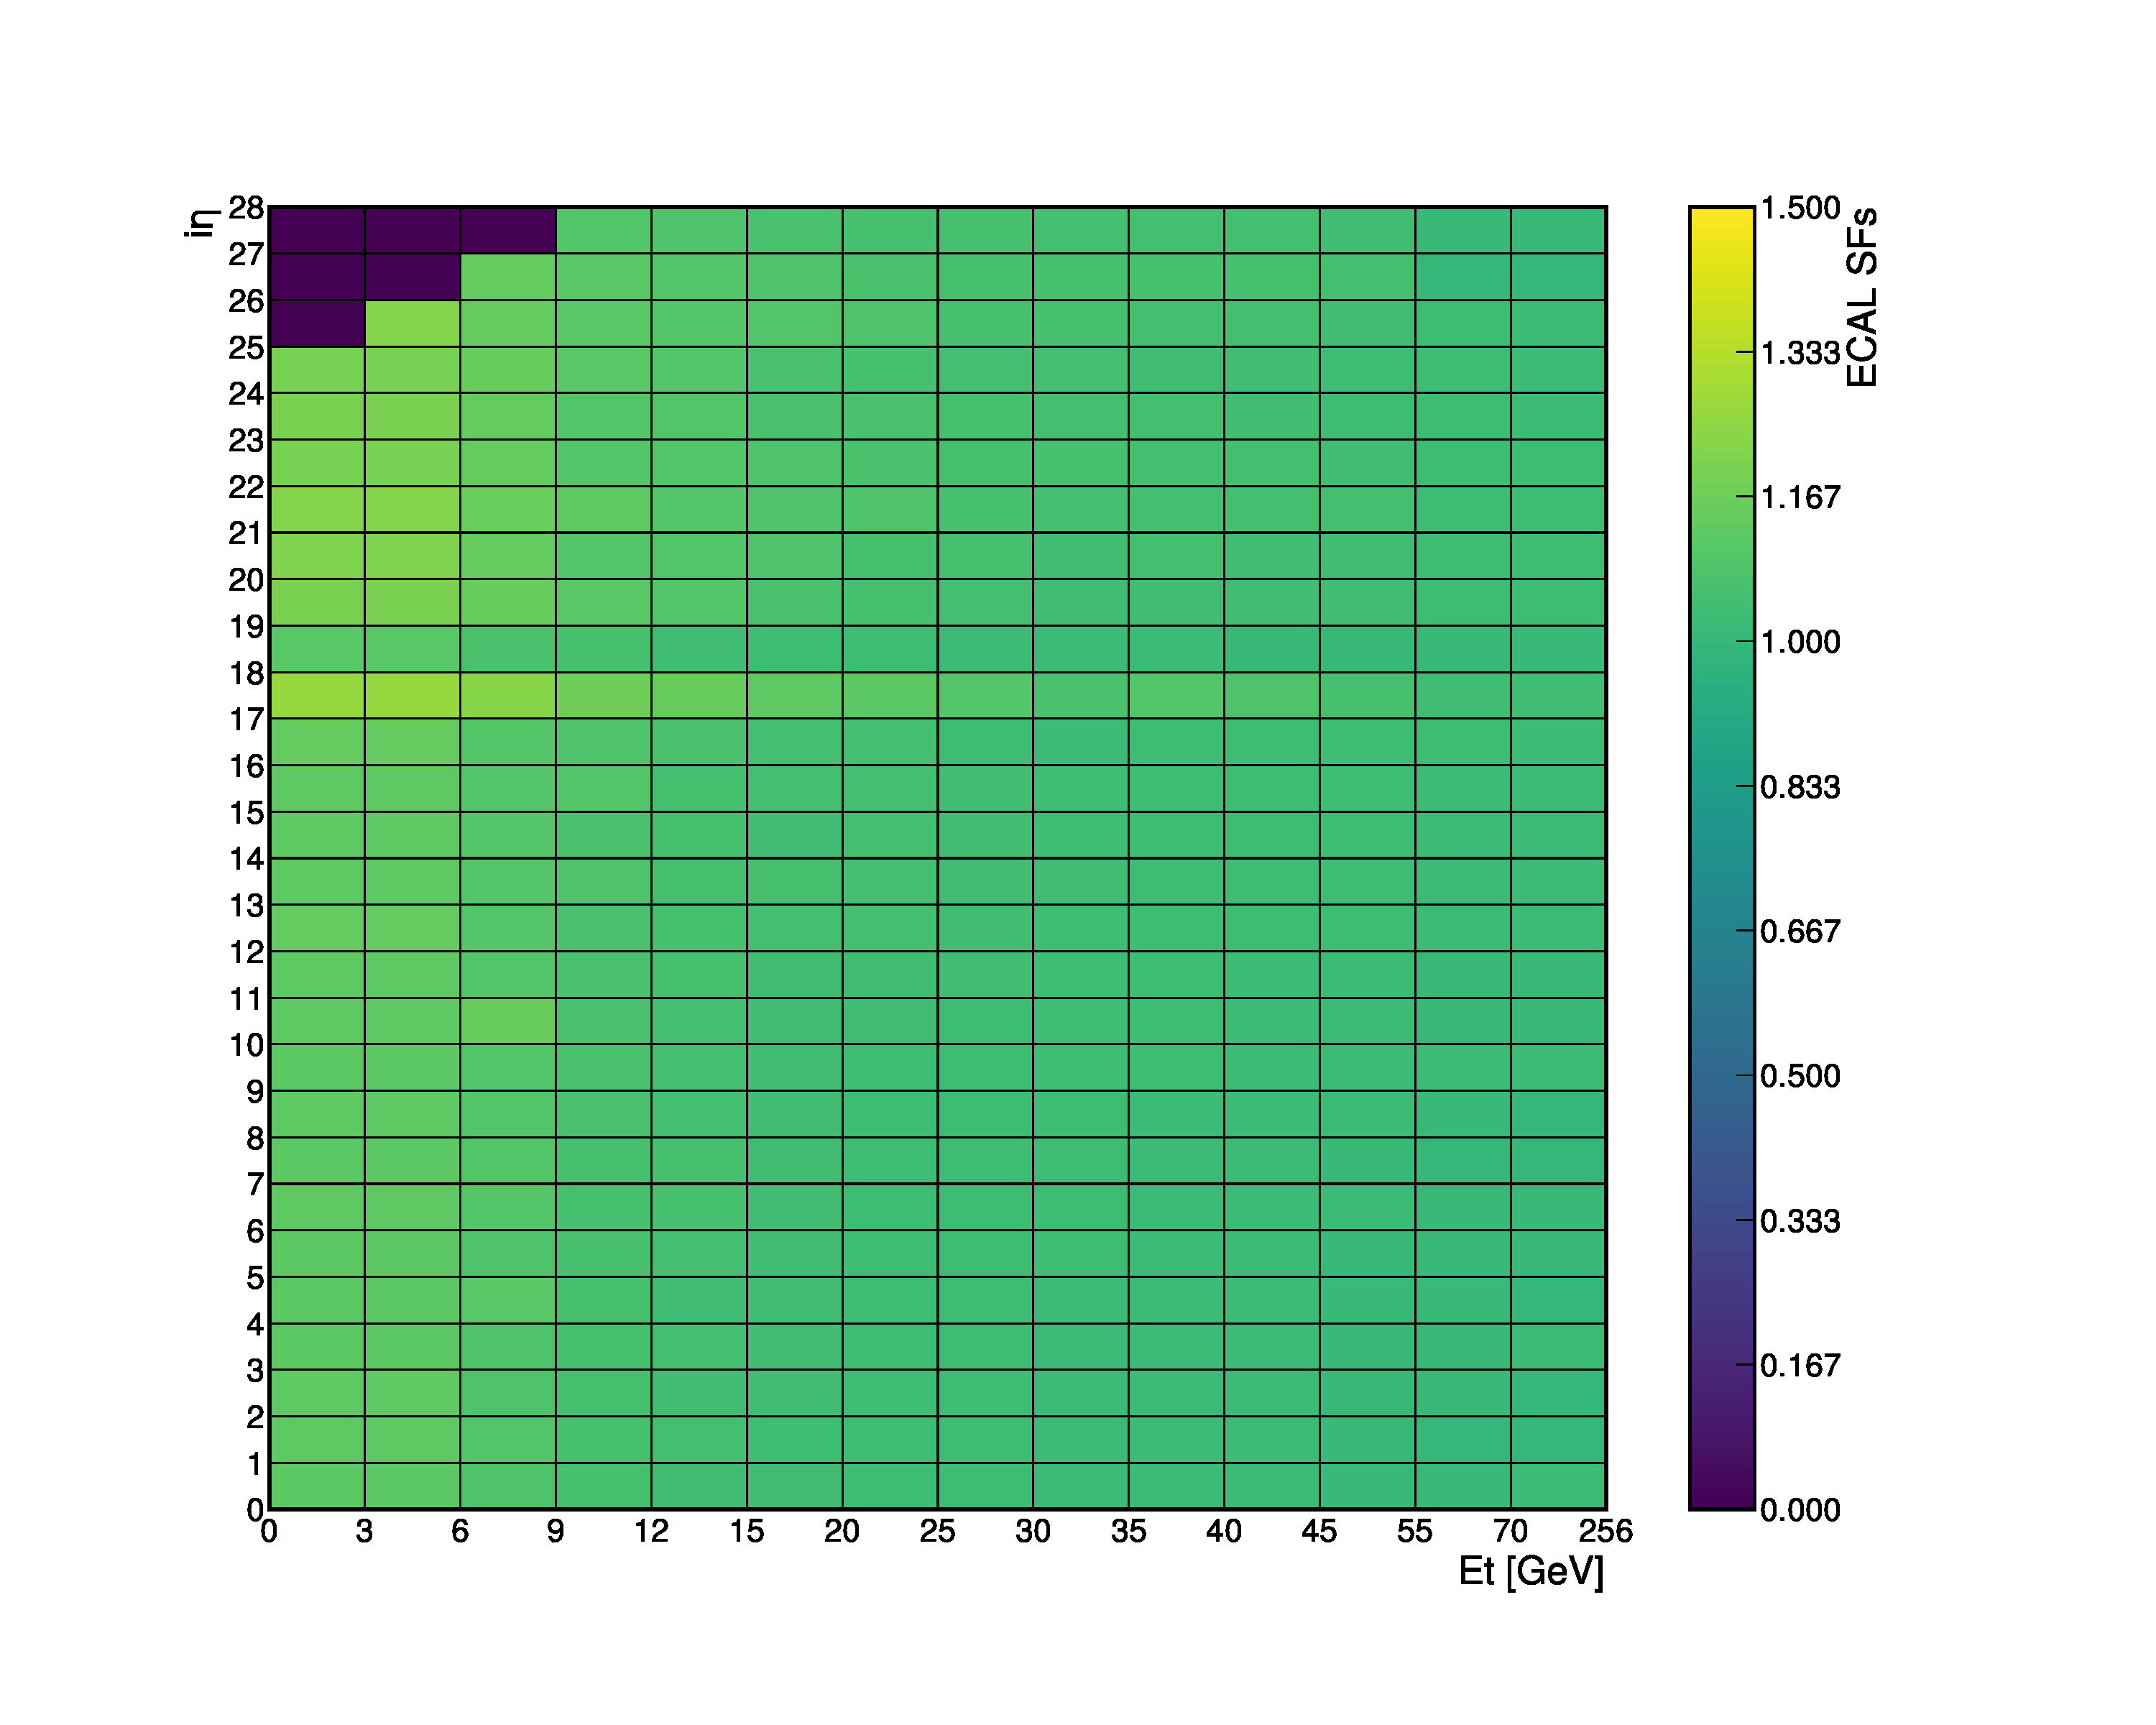
\includegraphics[width=0.5\linewidth]{Figures/L1TP/SFs_ECAL_before.pdf}}
    \subfloat[]{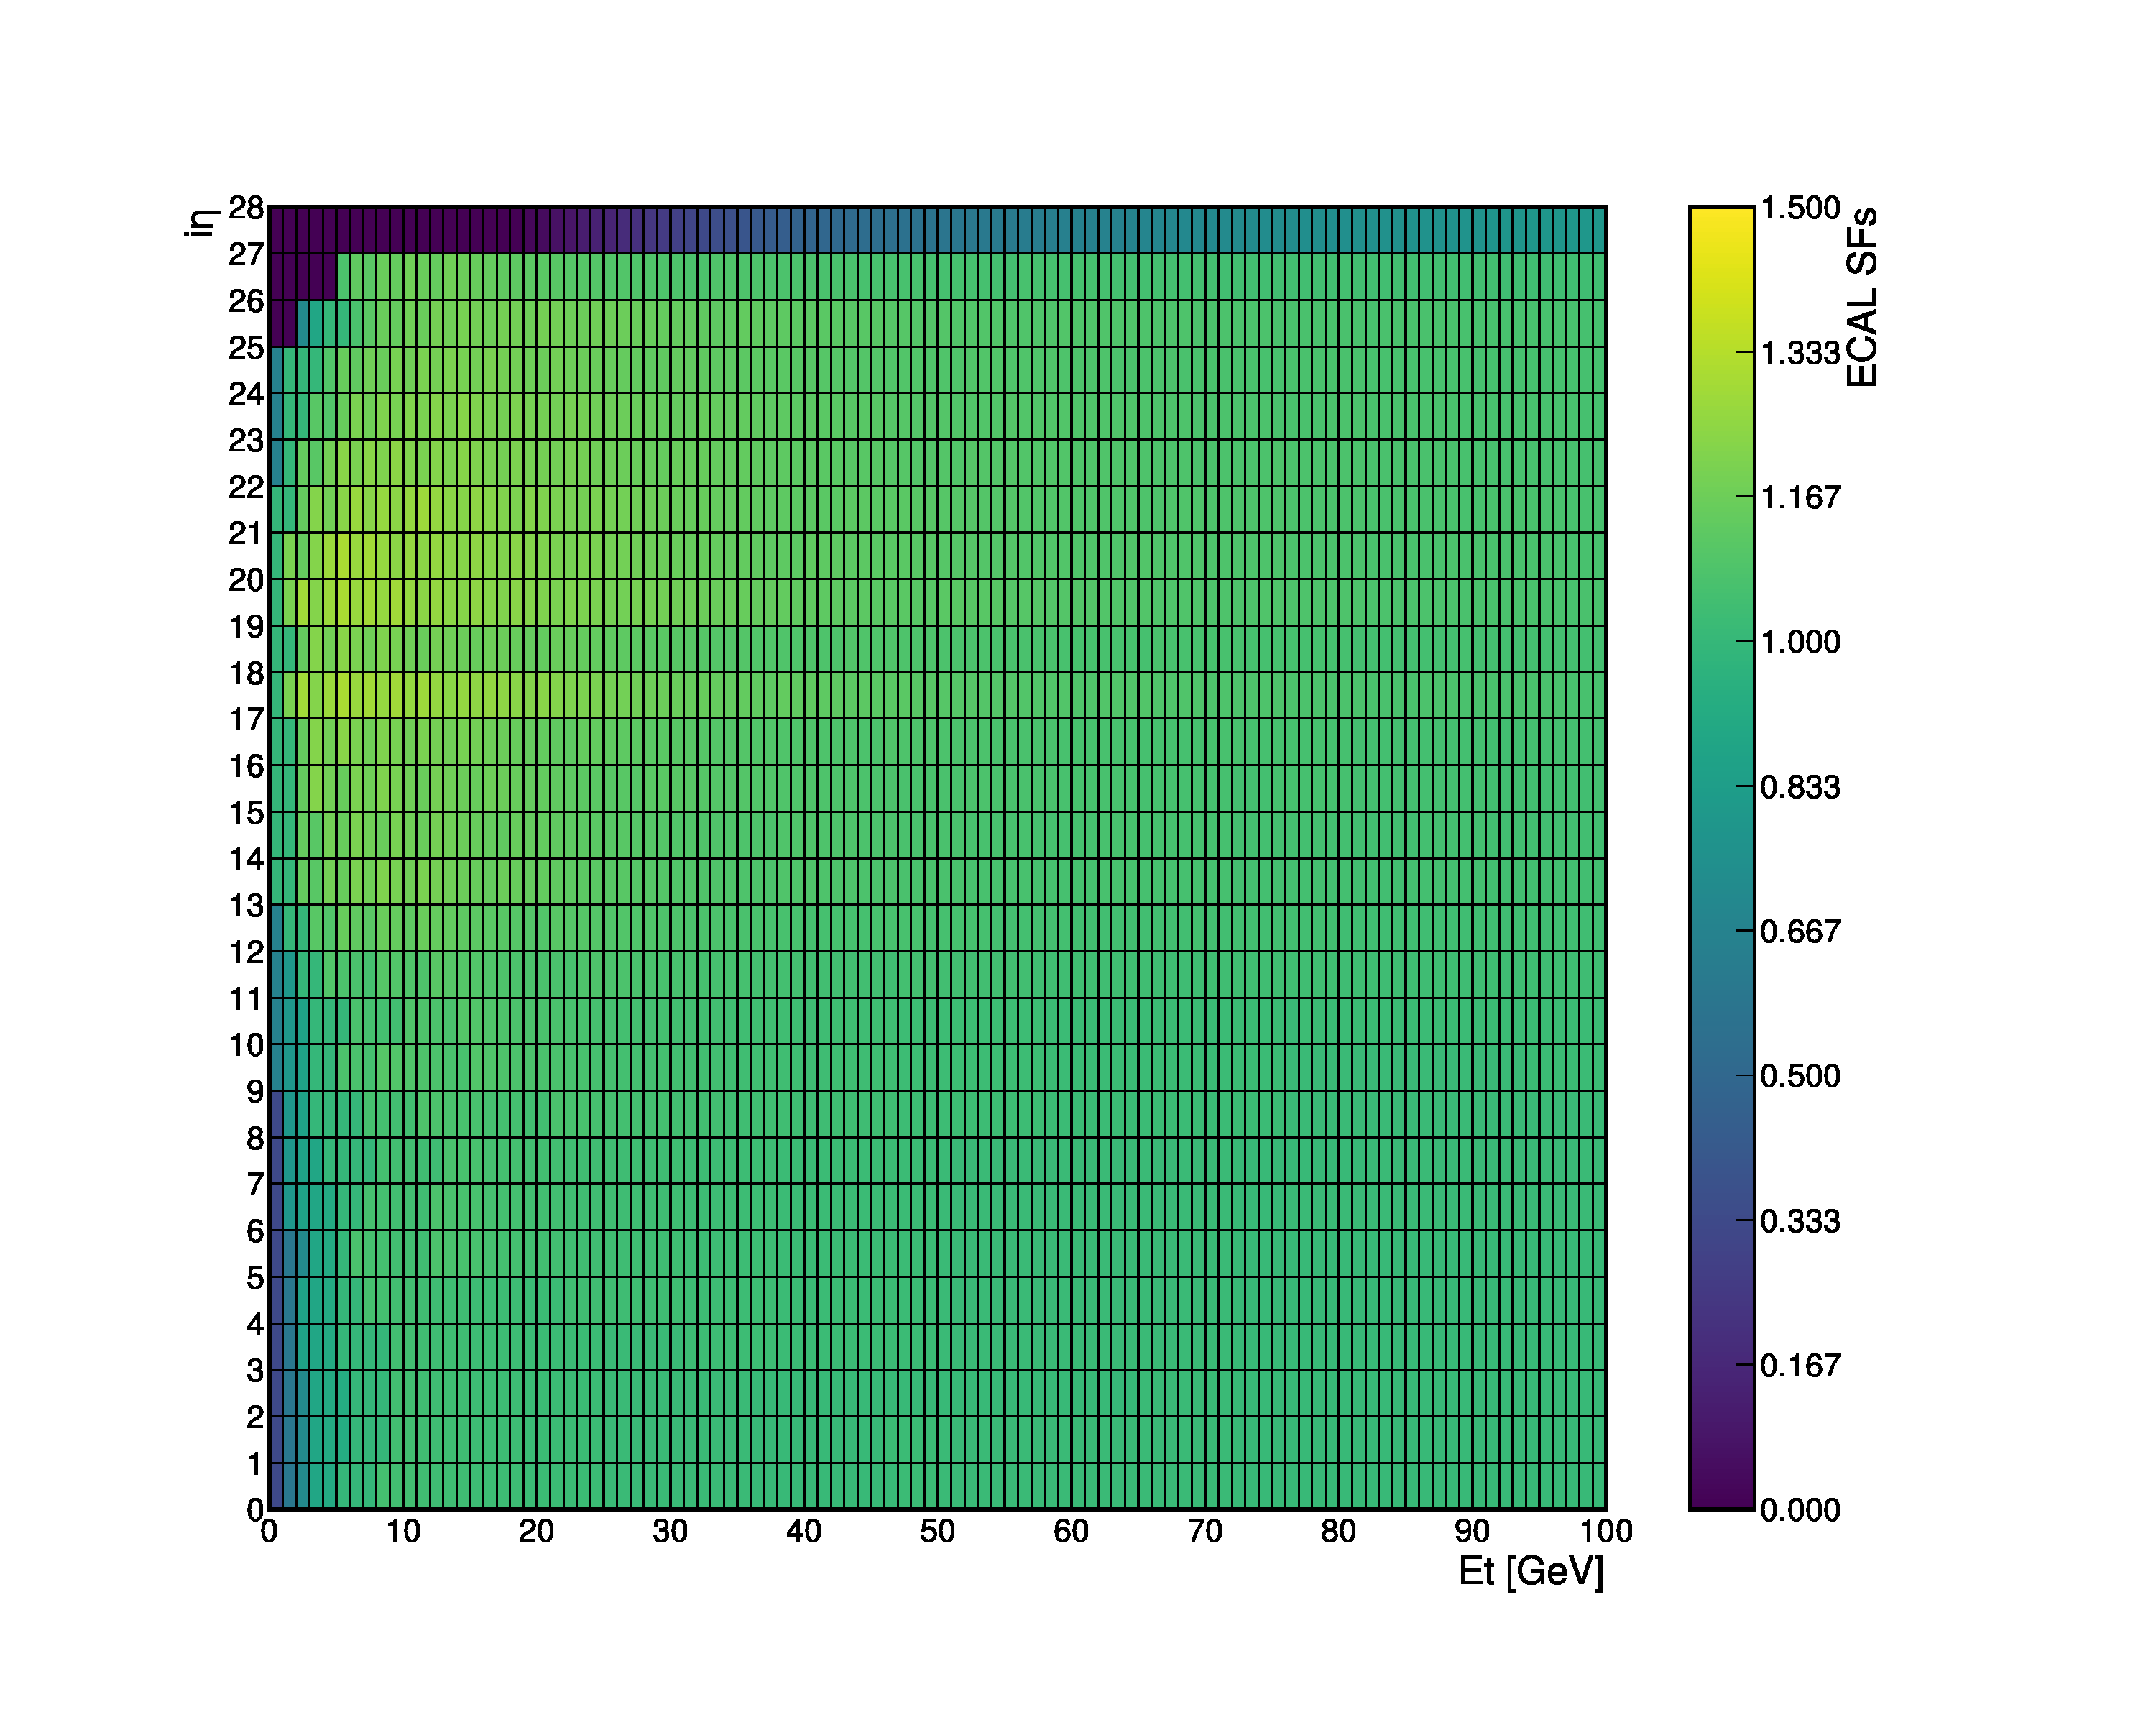
\includegraphics[width=0.5\linewidth]{Figures/L1TP/SFs_ECAL_now.pdf}}
    \caption{}
    \label{fig:ECALSFs_NN}
\end{figure}

\begin{figure}
    \centering
    \subfloat[]{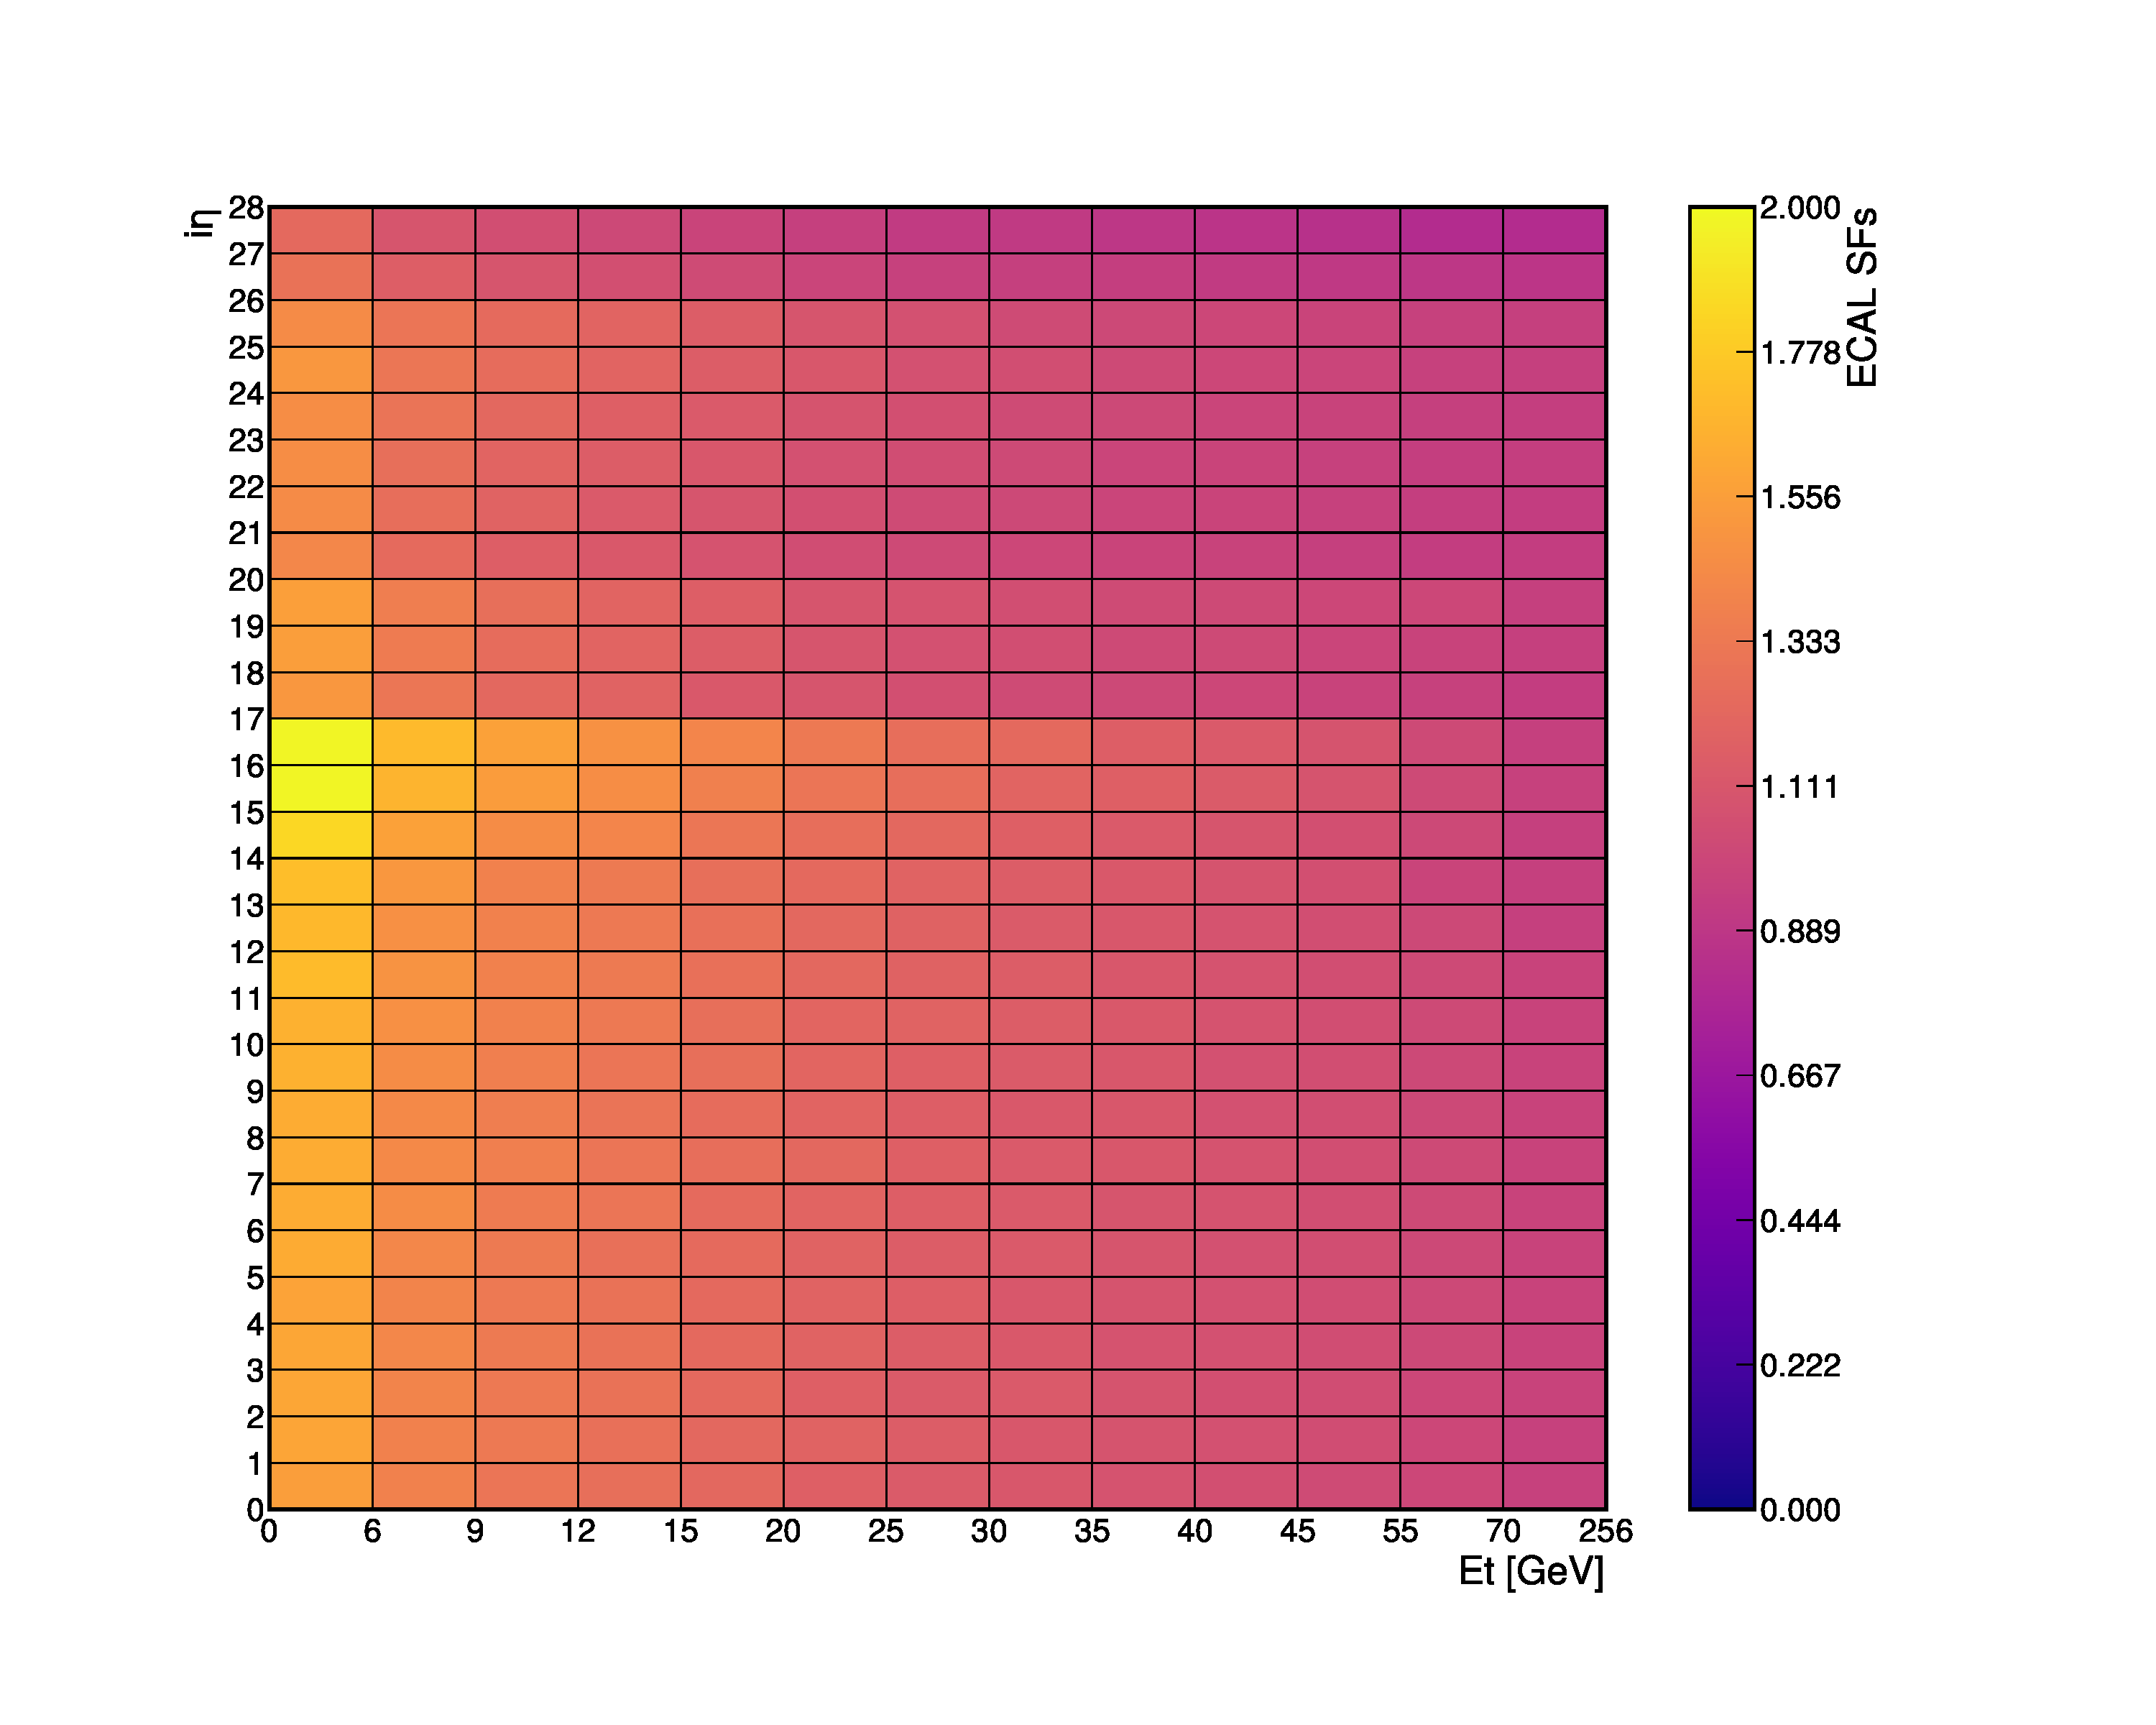
\includegraphics[width=0.5\linewidth]{Figures/L1TP/SFs_HCAL_before.pdf}}
    \subfloat[]{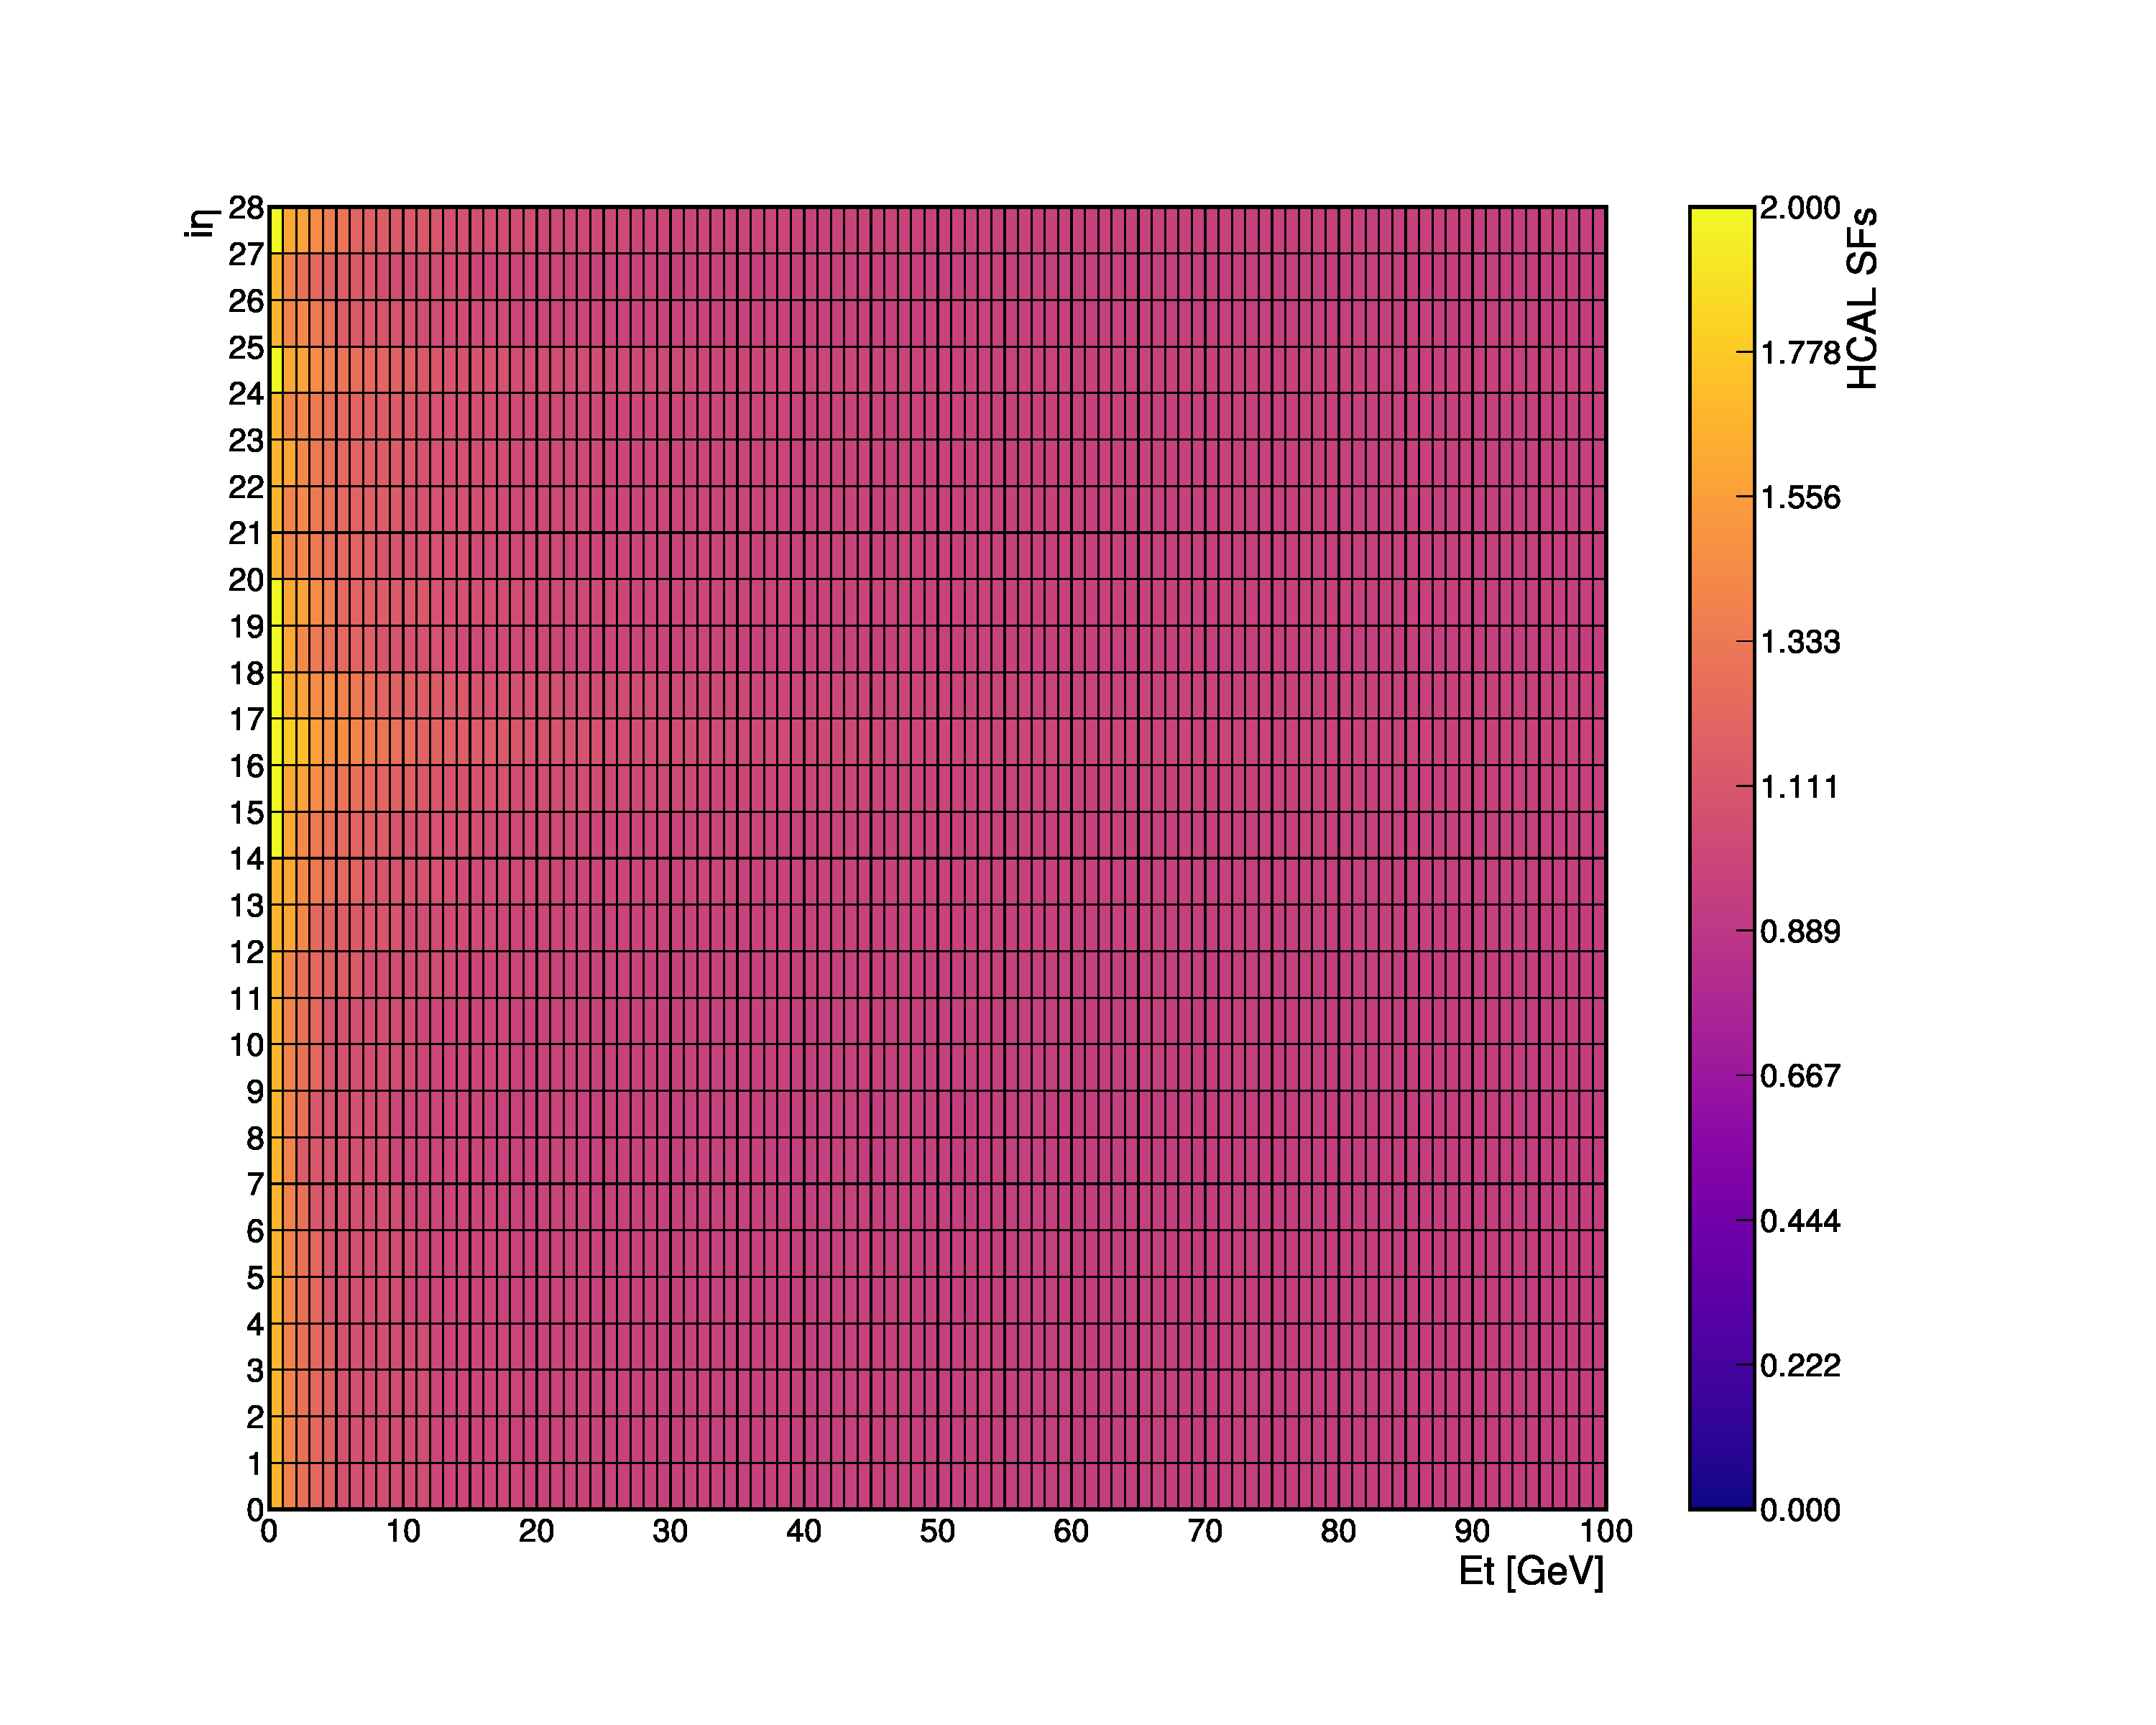
\includegraphics[width=0.5\linewidth]{Figures/L1TP/SFs_HCAL_now.pdf}}
    \caption{}
    \label{fig:HCALSFs_NN}
\end{figure}

\begin{figure}
    \centering
    \subfloat[]{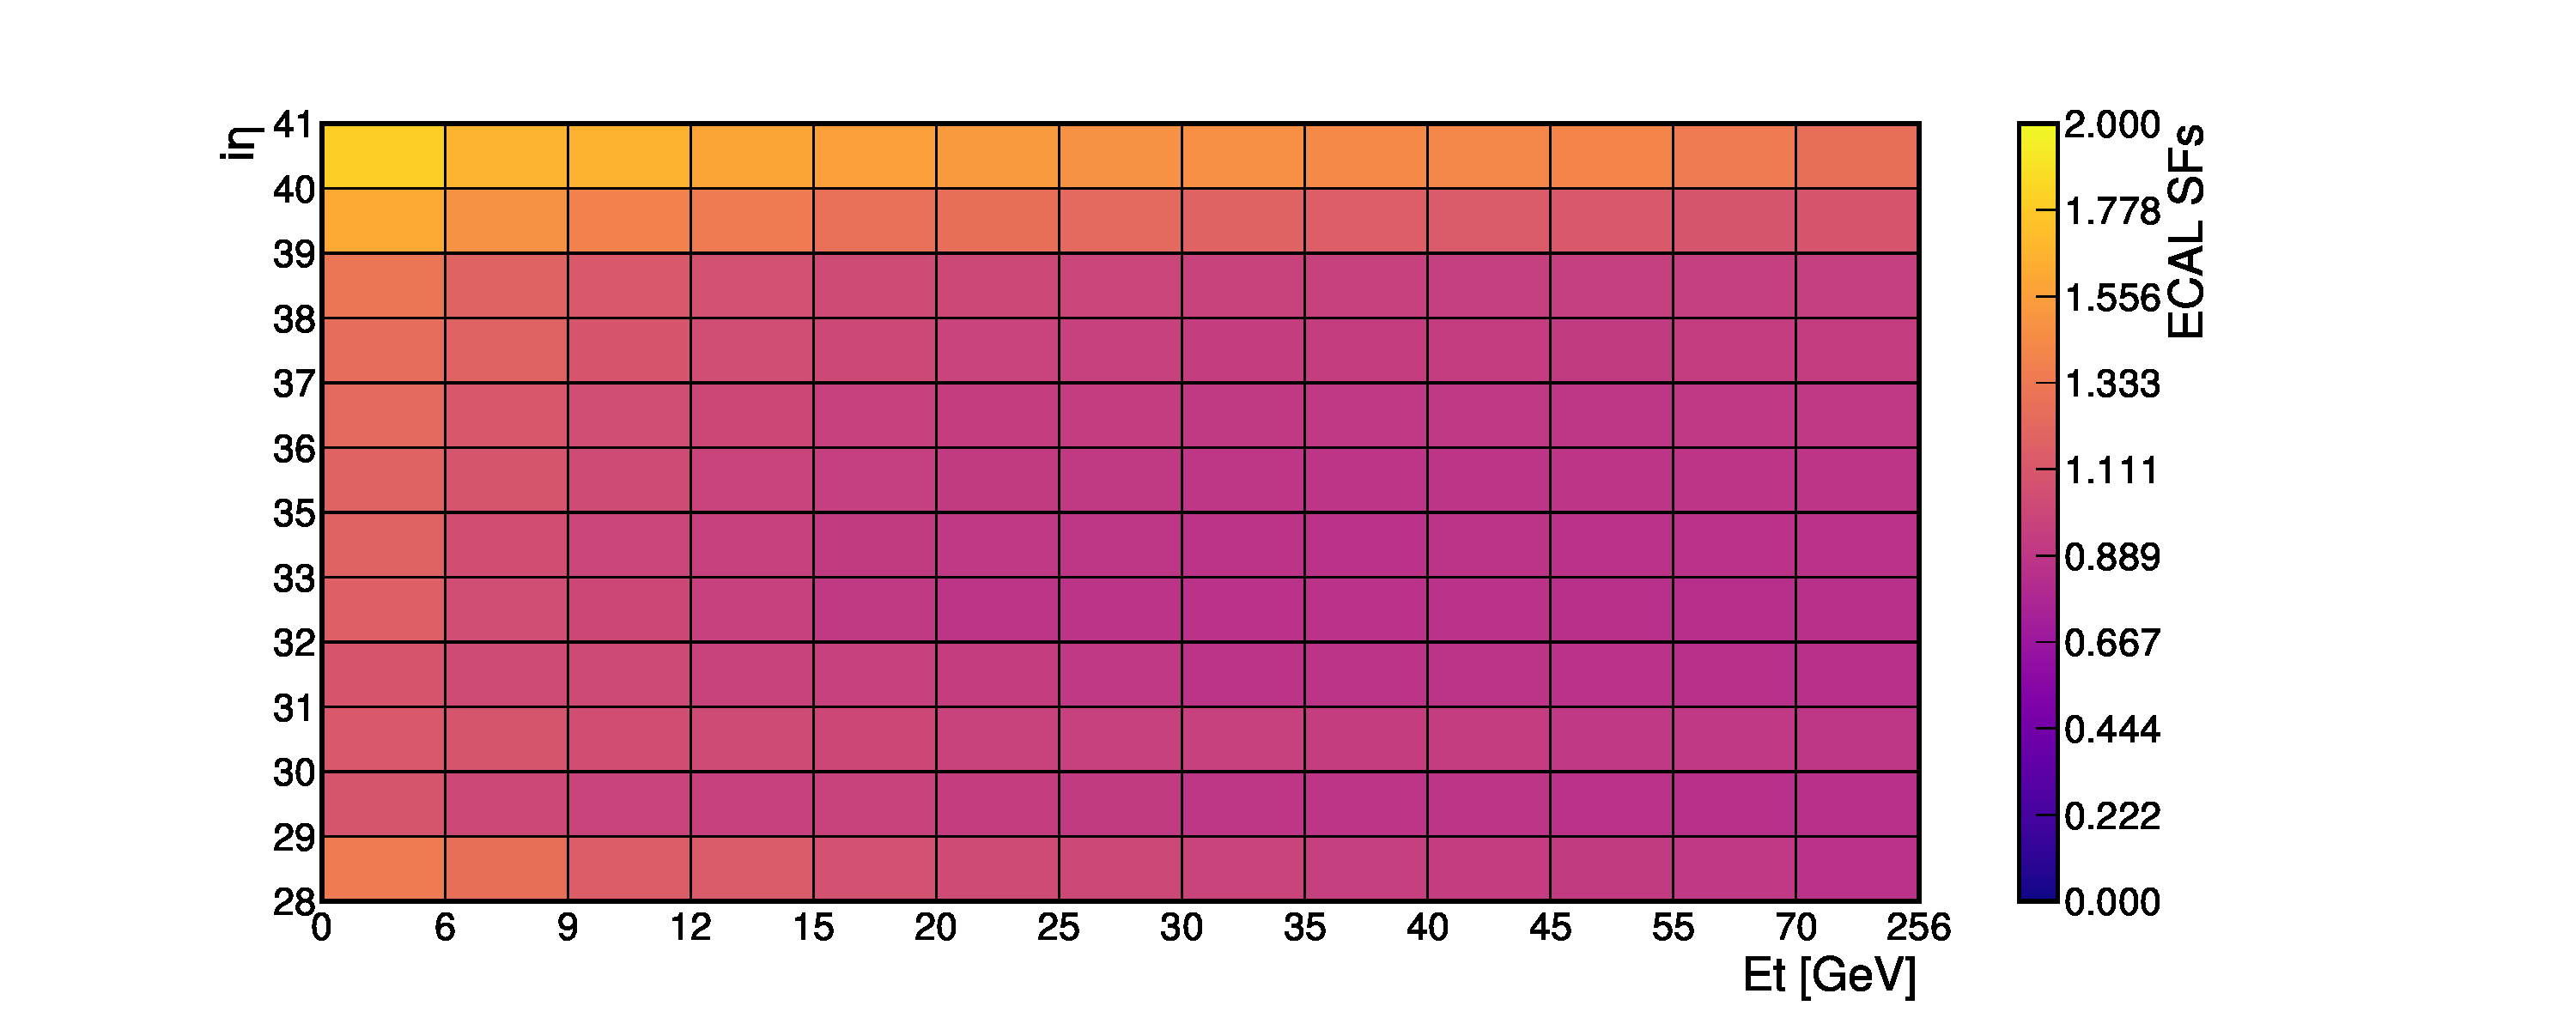
\includegraphics[width=0.5\linewidth]{Figures/L1TP/SFs_HF_before.pdf}}
    \subfloat[]{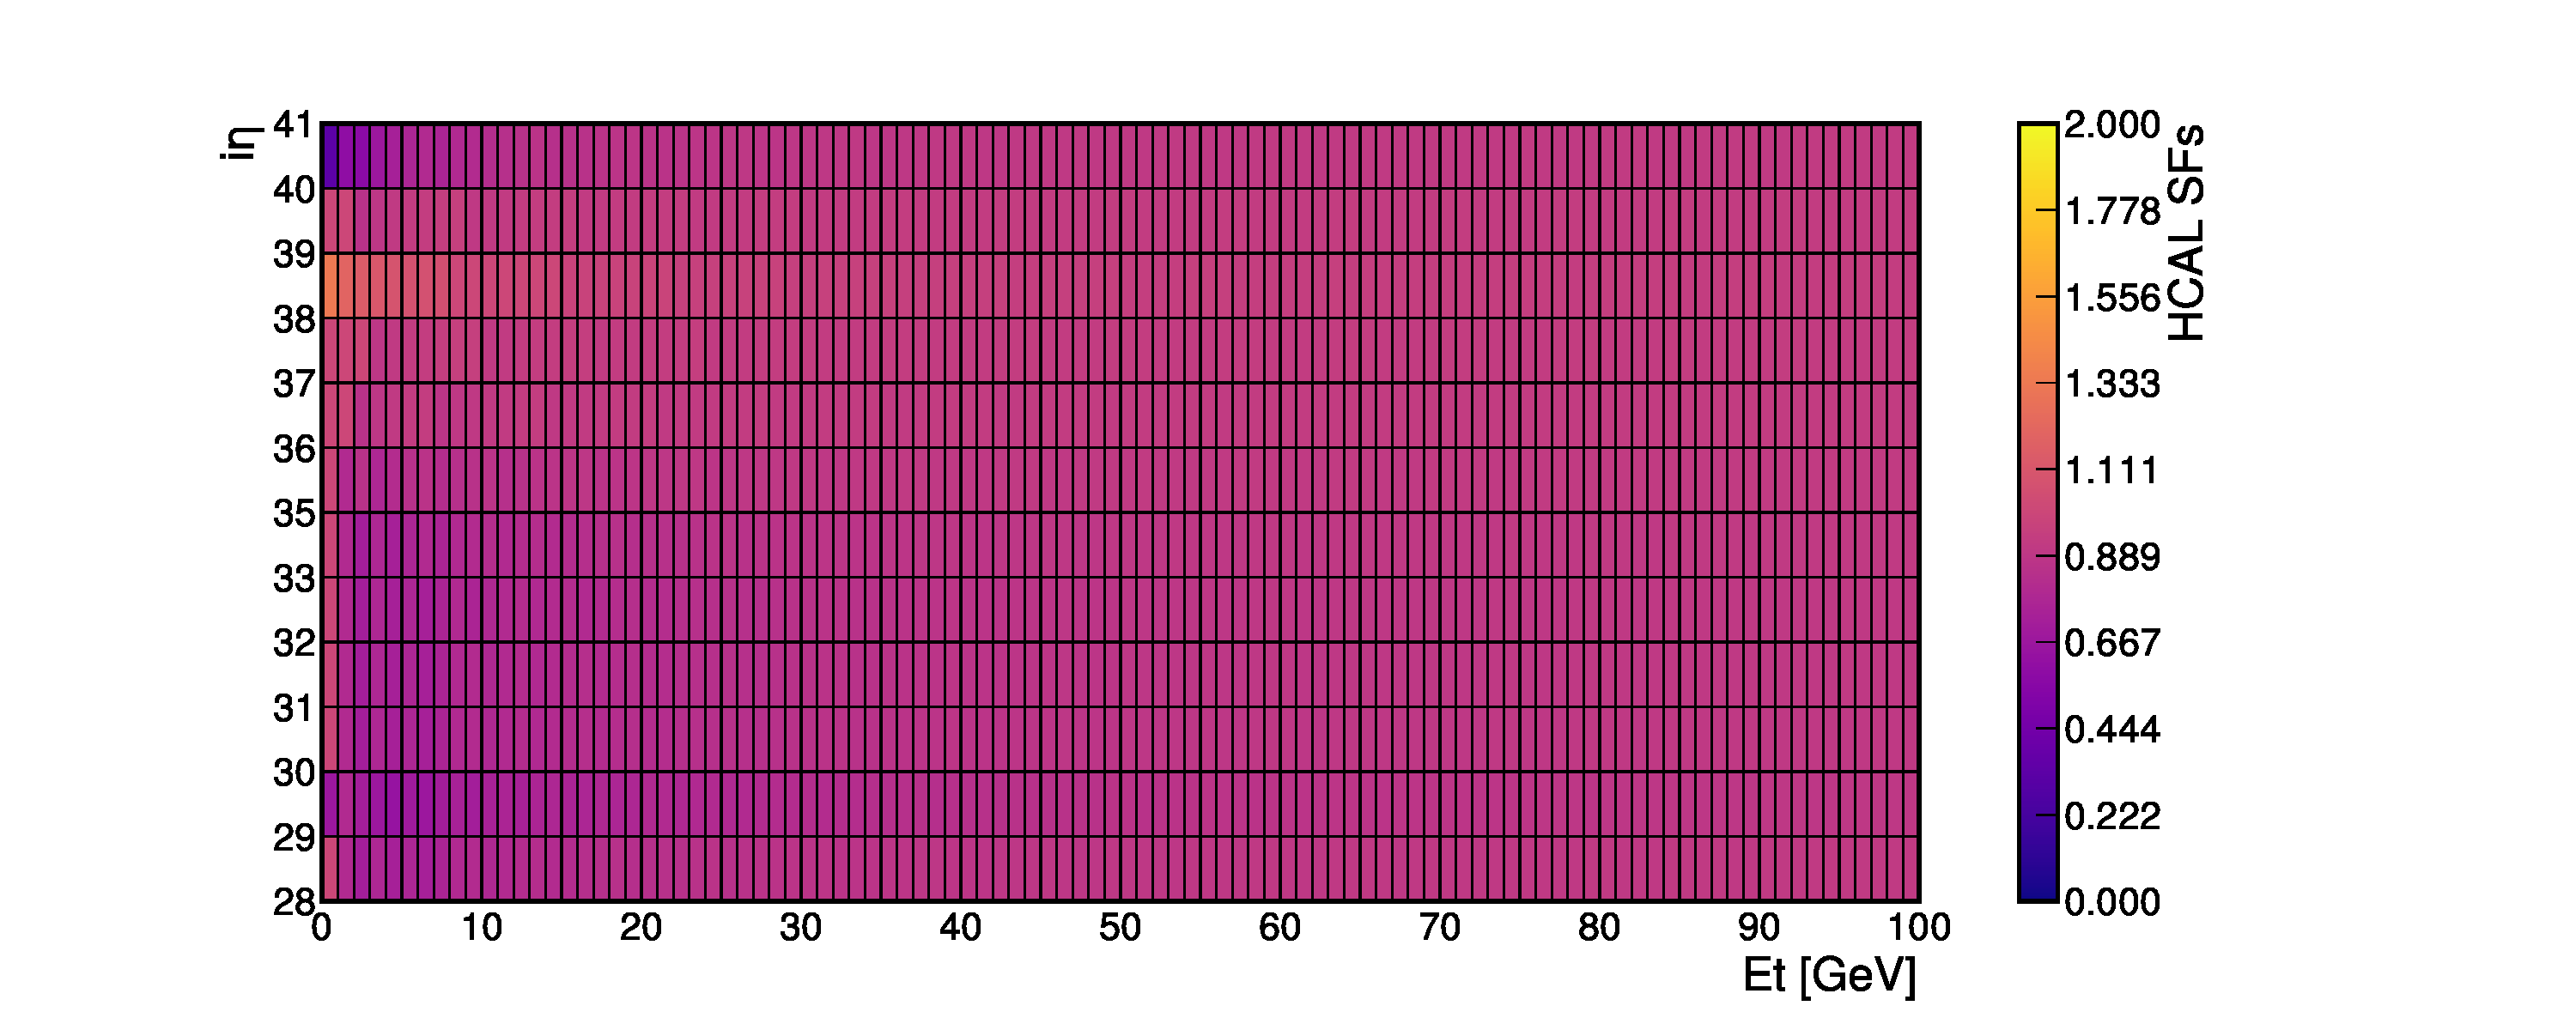
\includegraphics[width=0.5\linewidth]{Figures/L1TP/SFs_HF_now.pdf}}
    \caption{}
    \label{fig:HFSFs_NN}
\end{figure}

In the case of ECAL, the calibration factors are close to unity, with a slight suppression of TTs in the barrel recording low energy deposit, and a visible enhancement of TTs in the endcap. A discontinuity is noticeable for the region corresponding to $i\eta=18$, already present in the previous configuration of calibration factors: this region marks the transition from barrel to endcap, as shown in Figure~\ref{fig:Layer1}, where the depth of the ECAL crystals is reduced and a smaller energy deposit needs to be compensated by higher calibration factors. The six suppressed low energy towers corresponding to $i\eta=26,27,28$ are manually constrained to 0 in the extracted LUT, following Layer-1 recommendations, to reduce the impact of the most forward ECAL TTs, significantly affected by radiation damage.

In the case of HCAL, the calibration factors generally show larger values, especially for low energy TTs and in the region around $i\eta=17$, where the depth of HCAL crystals is reduced by the geometry of the detector. In the HF compartment, the newly derived calibration factors 
present a change with respect to the previous configuration, showing a tendency to suppress the TTs raw energy, by applying factors below unity. While the previous method was based on MC samples produced in the ideal environment of no pile-up, the NN is trained on real data, where the pile-up effect, which is predominant in the HF region, contaminates the L1 candidate: the NN learns how to suppress the additional energy contribution coming from pile-up and results in lower calibration factors across the HF region.

\bigbreak

% performance
The performance of the newly derived Layer-1 calibration factors can be evaluated by replicating the Layer-1 firmware implemented in the hardware of the CMS service cavern with the new LUTs. A dataset collected by the CMS experiment during Run~III data taking is re-emulated under three different Layer-1 configurations: one in which no calibration is applied (\textit{No calibration}), one in which the calibration factors are set to the values obtained with the old method (\textit{Old calibration}), and one in which the calibration constants are derived with the NN approach presented in this section (\textit{New calibration}).
The three configurations are compared in terms of Layer-1 energy response, defined as the ratio between the L1 $e/\gamma$ or jet candidate energy and the offline reconstructed electron of PUPPI jet energy. From the differential distribution of the Layer-1 energy response, the mean of the distribution defines the energy scale, which is expected to be as close as possible to unity, while the ratio between the standard deviation and the mean defines the energy resolution, which needs to be minimised for a performance improvement.
However, the resolution is only a partial aspect of the Layer-1 trigger performance, which has to be evaluated in terms of expected rate and efficiency. A commonly used figure of merit for the L1 performance evaluation is the efficiency turn-on curve, which describes, for a given L1-$p_T$ threshold, the efficiency in detecting and reconstructing the L1 candidates that are correctly matched to offline candidates with the same energy. The efficiency turn-on curve is computed as the ratio between offline-$p_T$ distribution of the objects matched to a L1 candidate passing the L1-$p_T$ threshold and the offline-$p_T$ distribution of all offline objects. 
Ideally, the efficiency turn-on curve should be centered around the L1-$p_T$ threshold, with minimum efficiency for objects below the thresholds and maximum efficiency above the threshold. 
In reality, the definition of the L1 energy is not always accurate, given the reduced information available, and can be either under-estimated or over-estimated, leading potential inefficiencies or false positives and resulting in a less steep turn-on curve.
To account for differences in the rate and ensure a fair comparison of the different methods, the efficiency turn-on curves computed for L1-$p_T$ thresholds providing the same Layer-1 rate are compared to each other.

\bigbreak

\begin{figure}
    \centering
    \subfloat[]{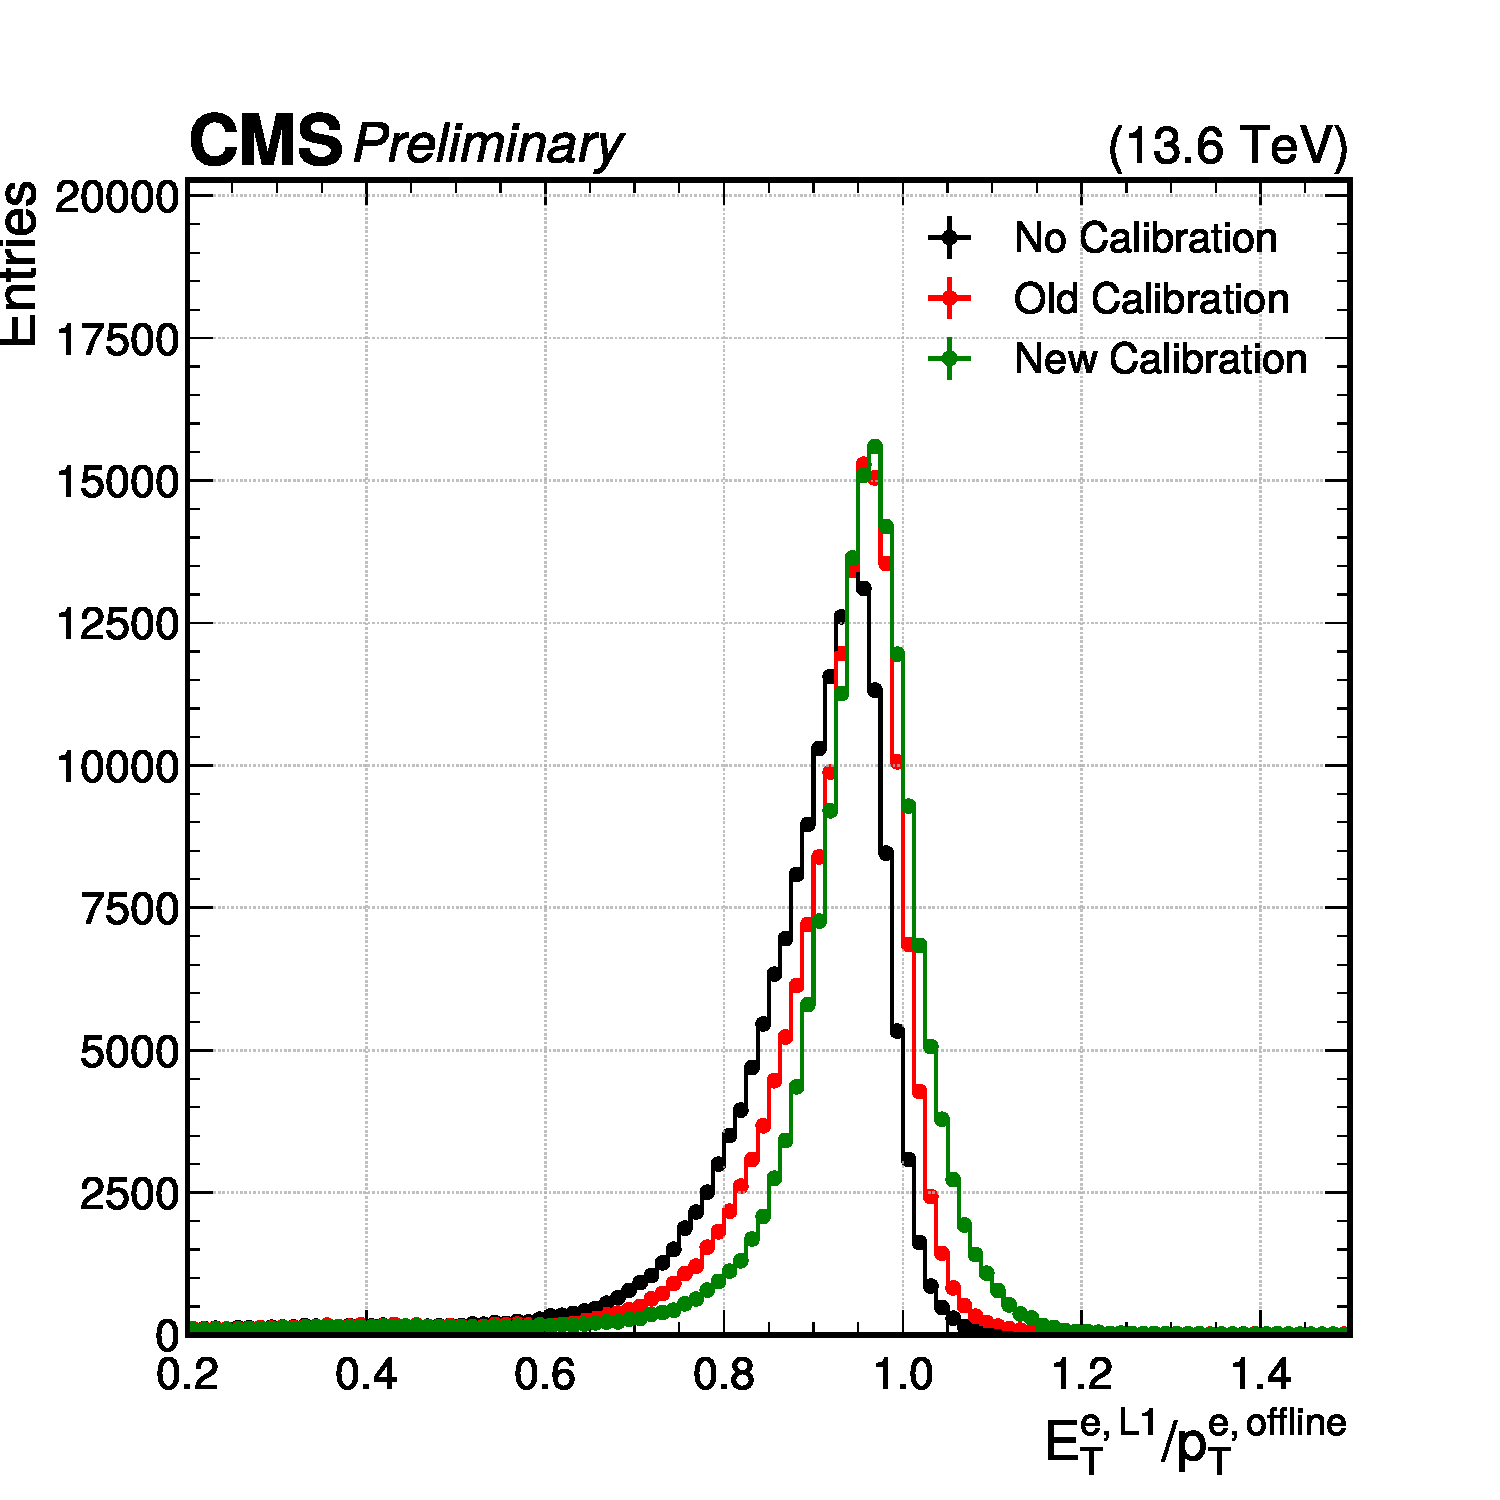
\includegraphics[width=0.5\linewidth]{Figures/L1TP/NN_Performance/response_inclusive__ele.pdf}}
    
    \subfloat[]{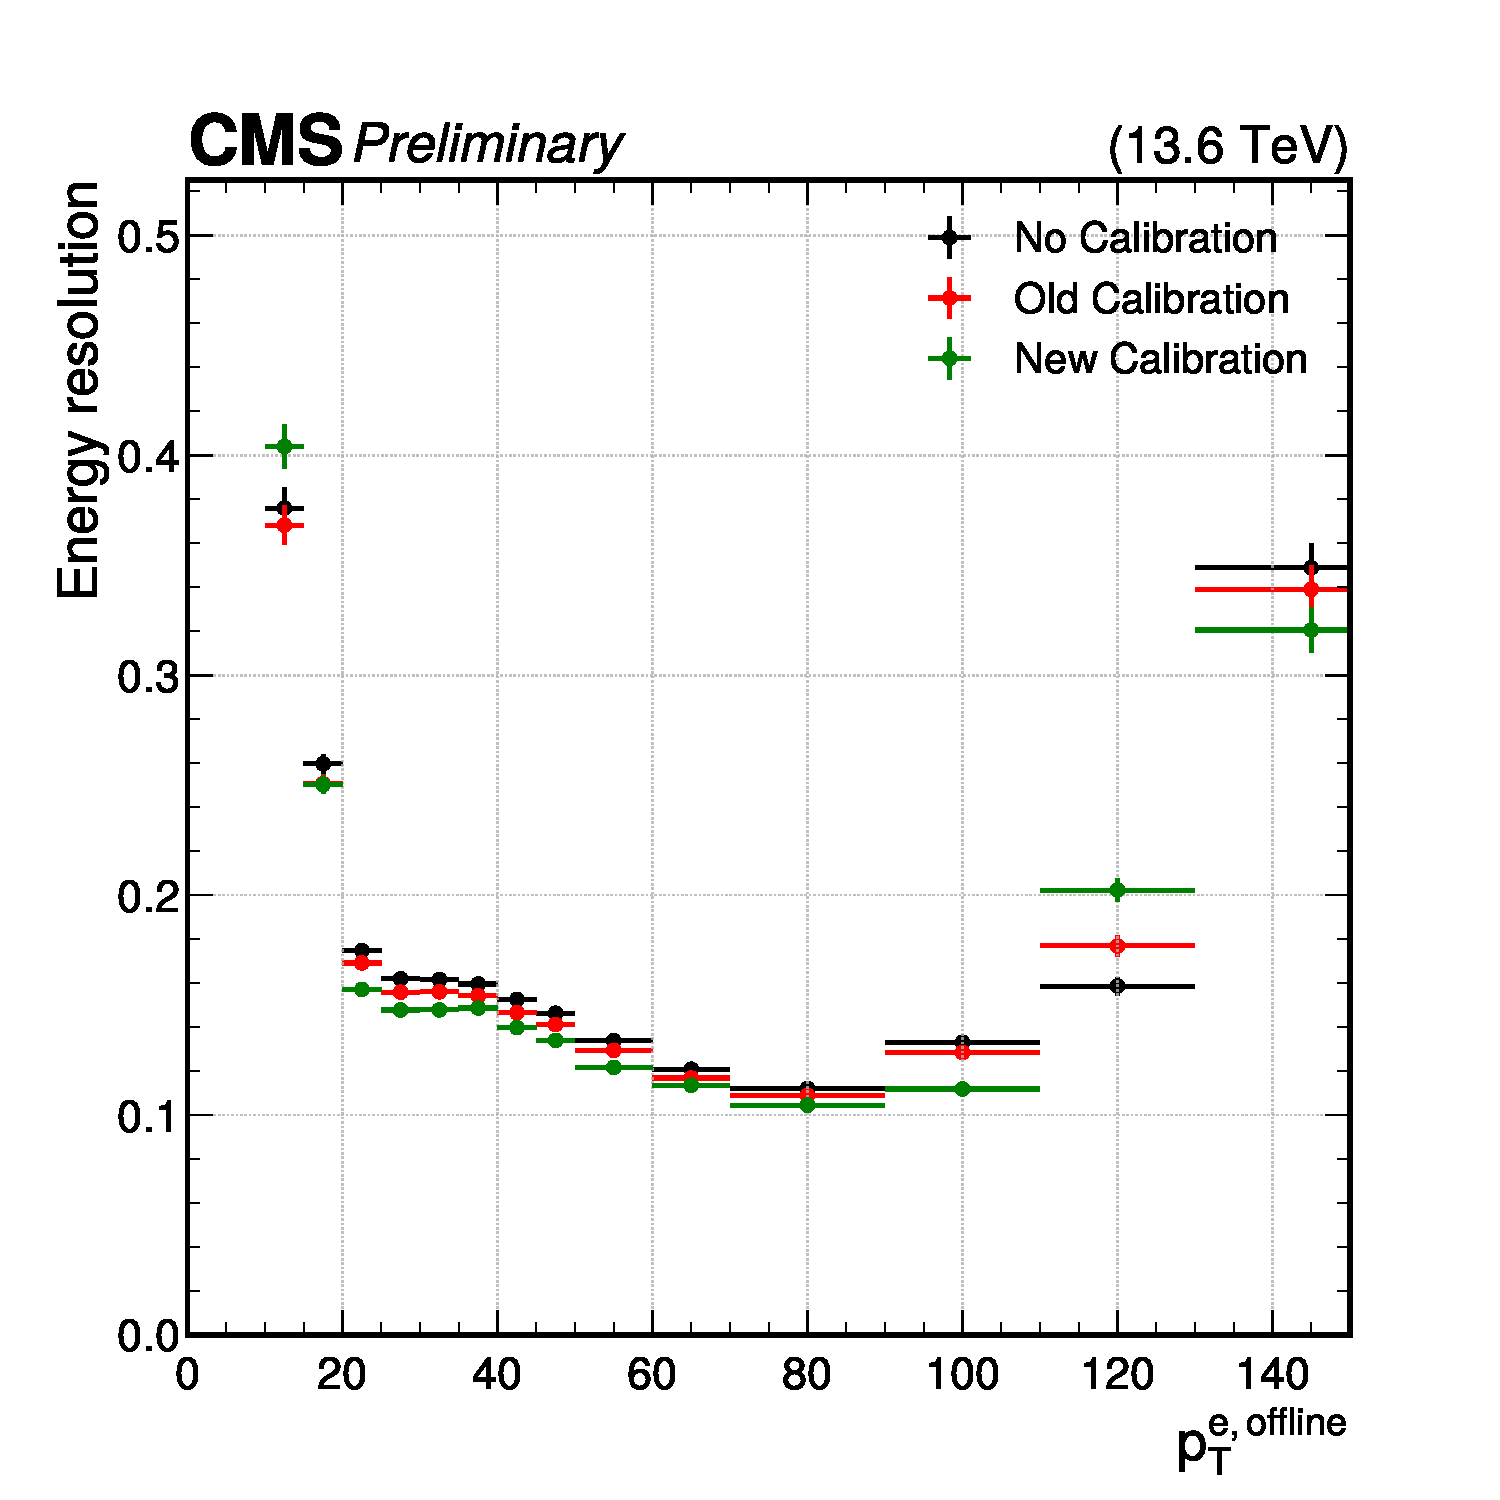
\includegraphics[width=0.5\linewidth]{Figures/L1TP/NN_Performance/resolution_ptBins__ele.pdf}}
    \subfloat[]{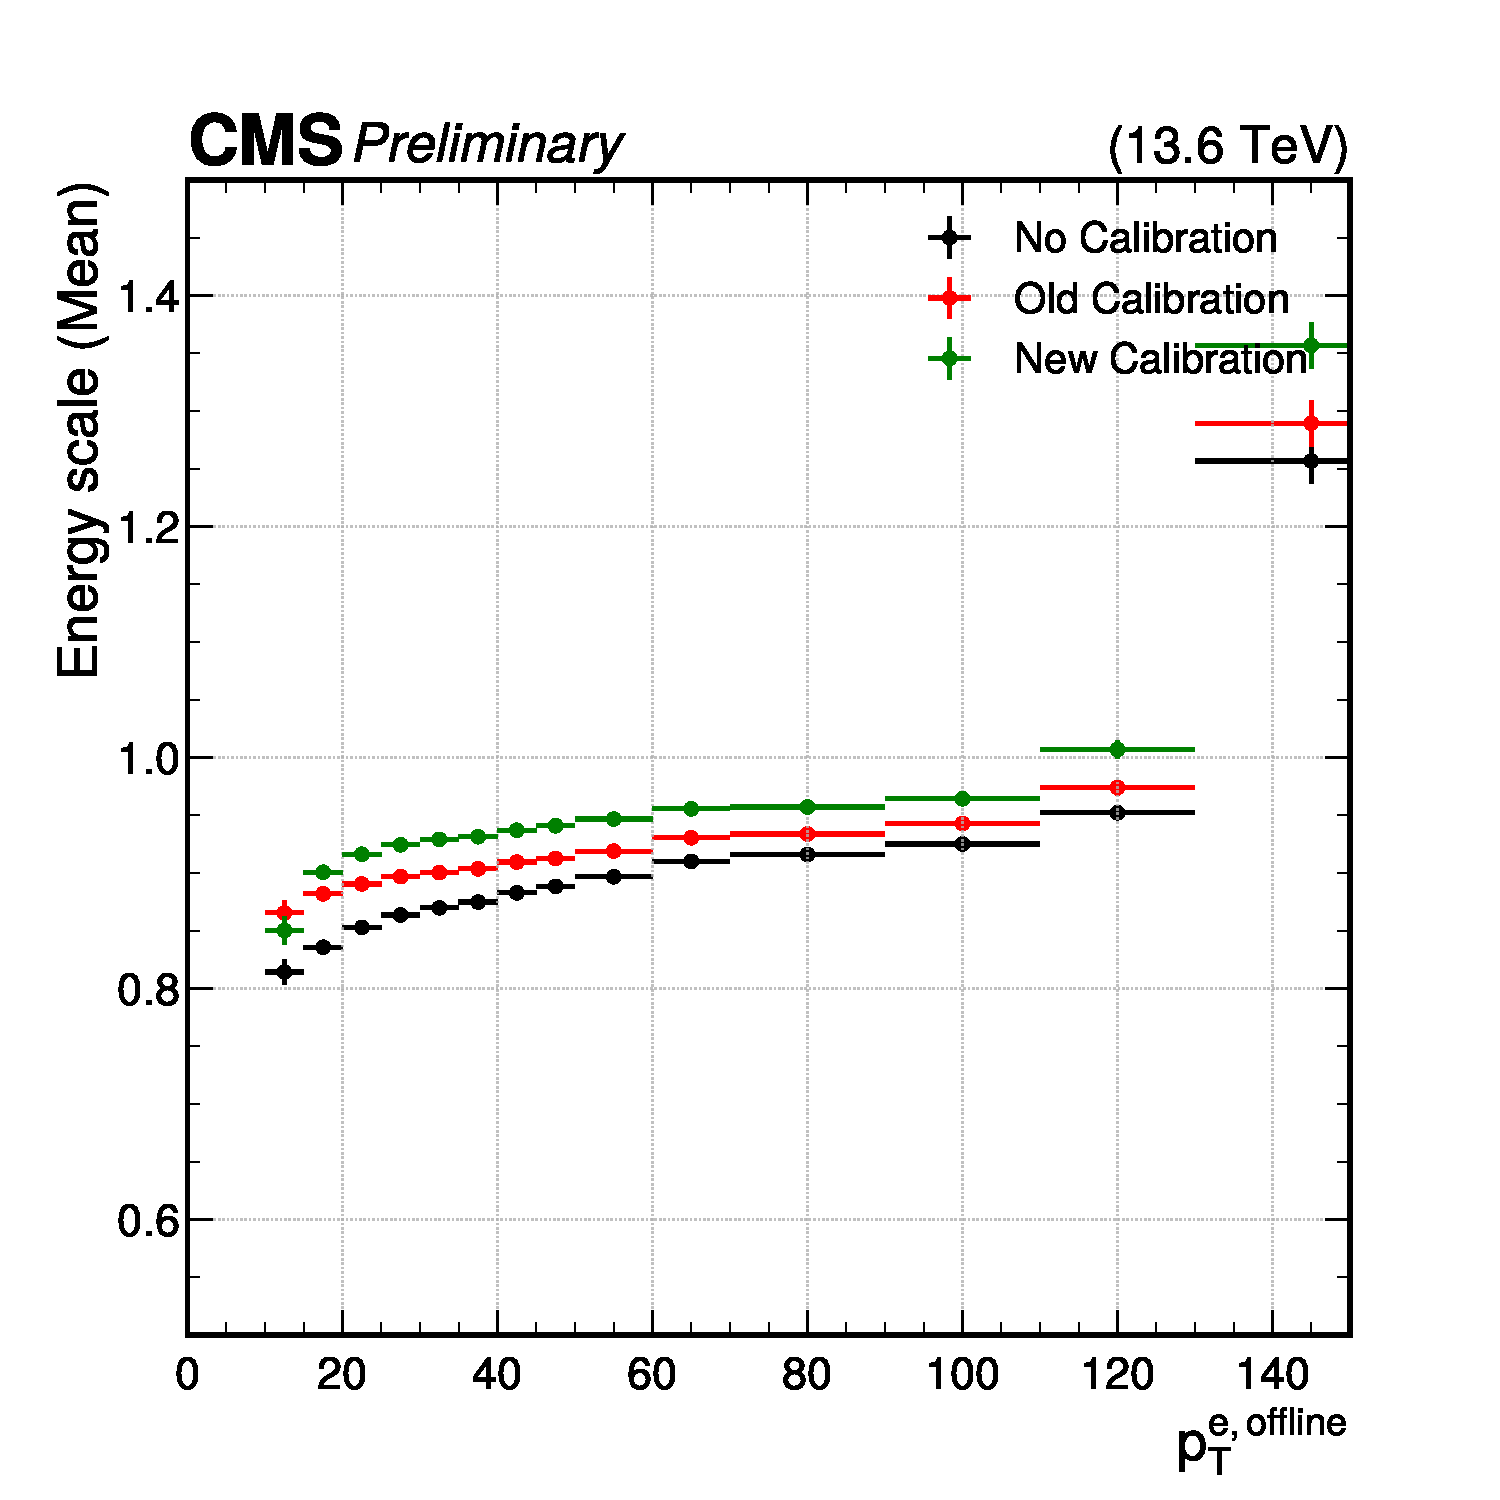
\includegraphics[width=0.5\linewidth]{Figures/L1TP/NN_Performance/scale_ptBins__ele.pdf}}
    \caption{}
    \label{fig:NN_ECAL_Response}
\end{figure}

\begin{figure}
    \centering
    \subfloat[]{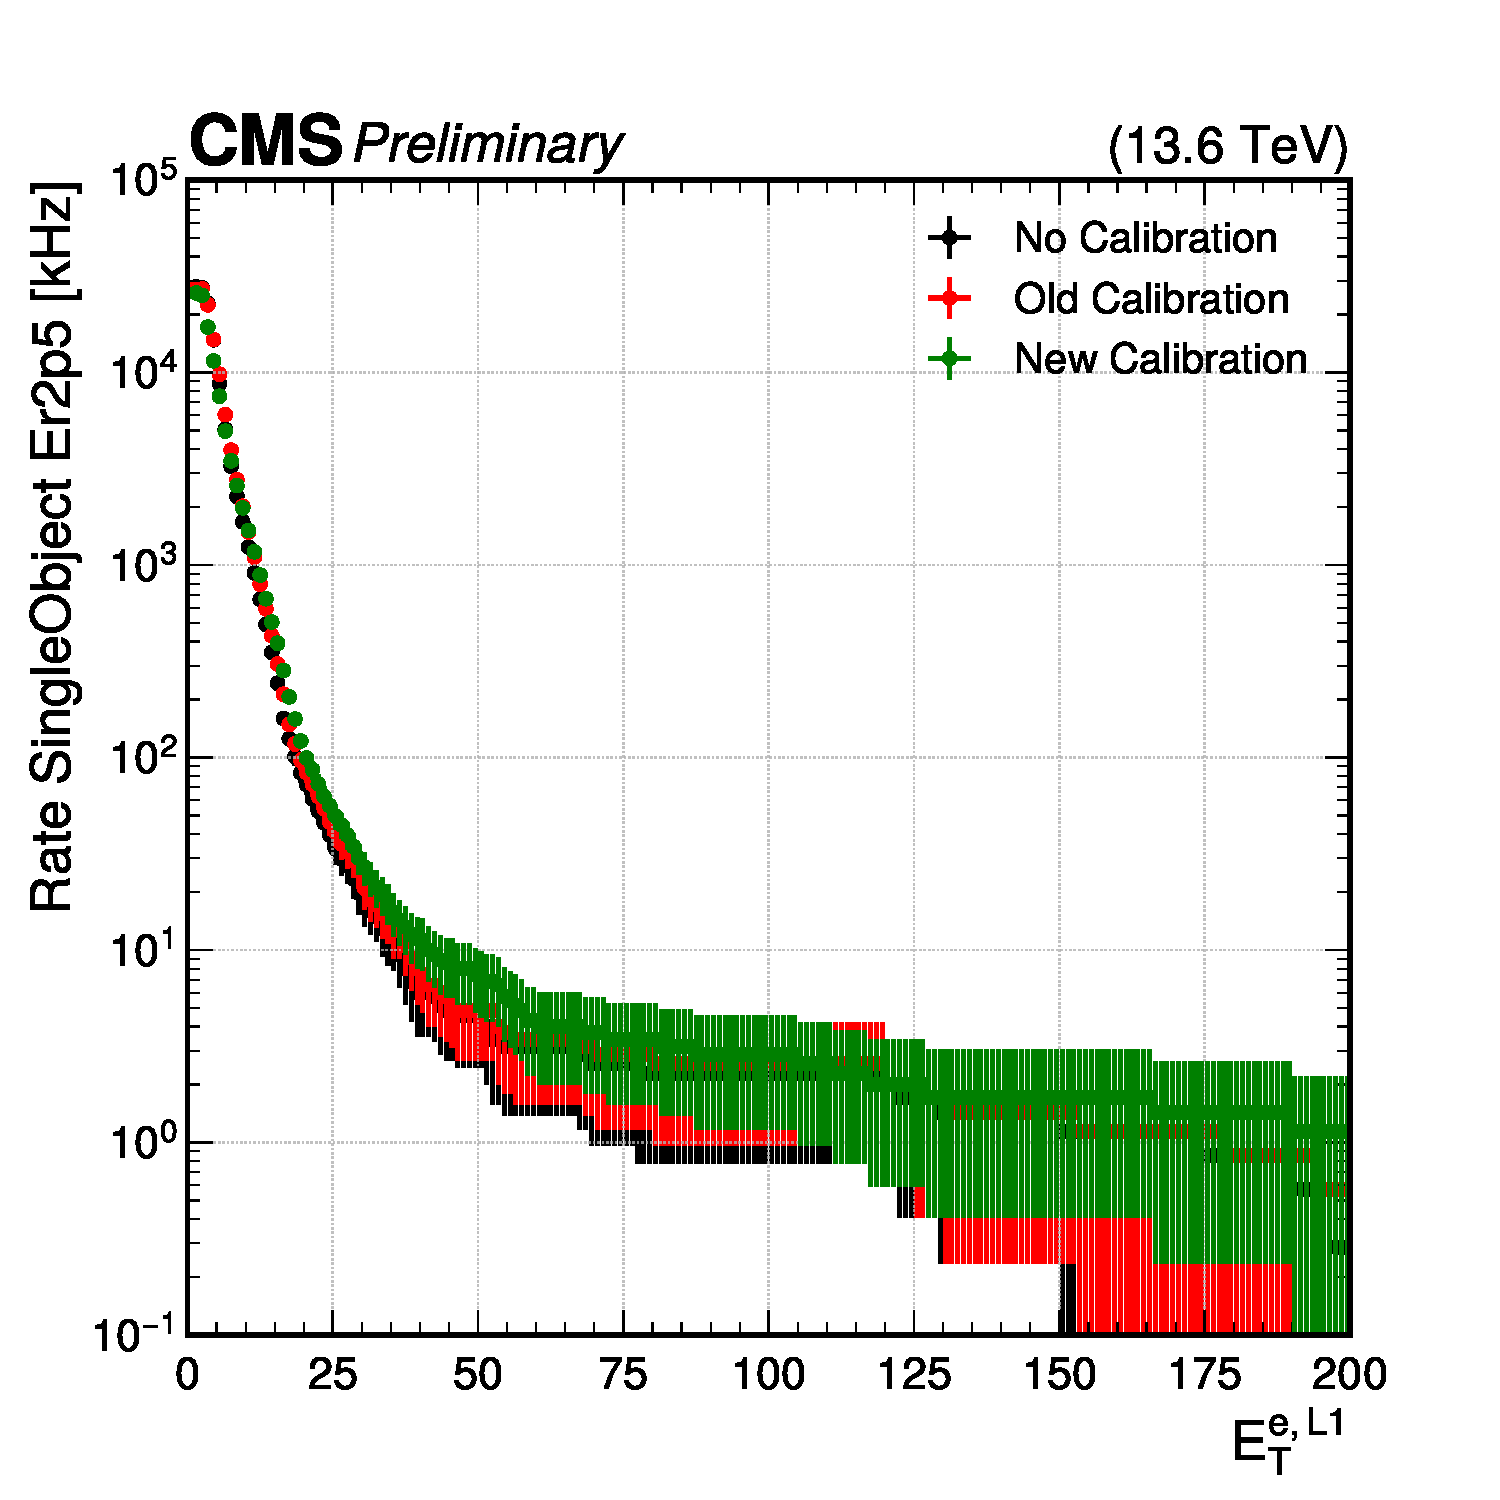
\includegraphics[width=0.5\linewidth]{Figures/L1TP/NN_Performance/rate_ObjEr2p5__ele.pdf}}
    
    \subfloat[]{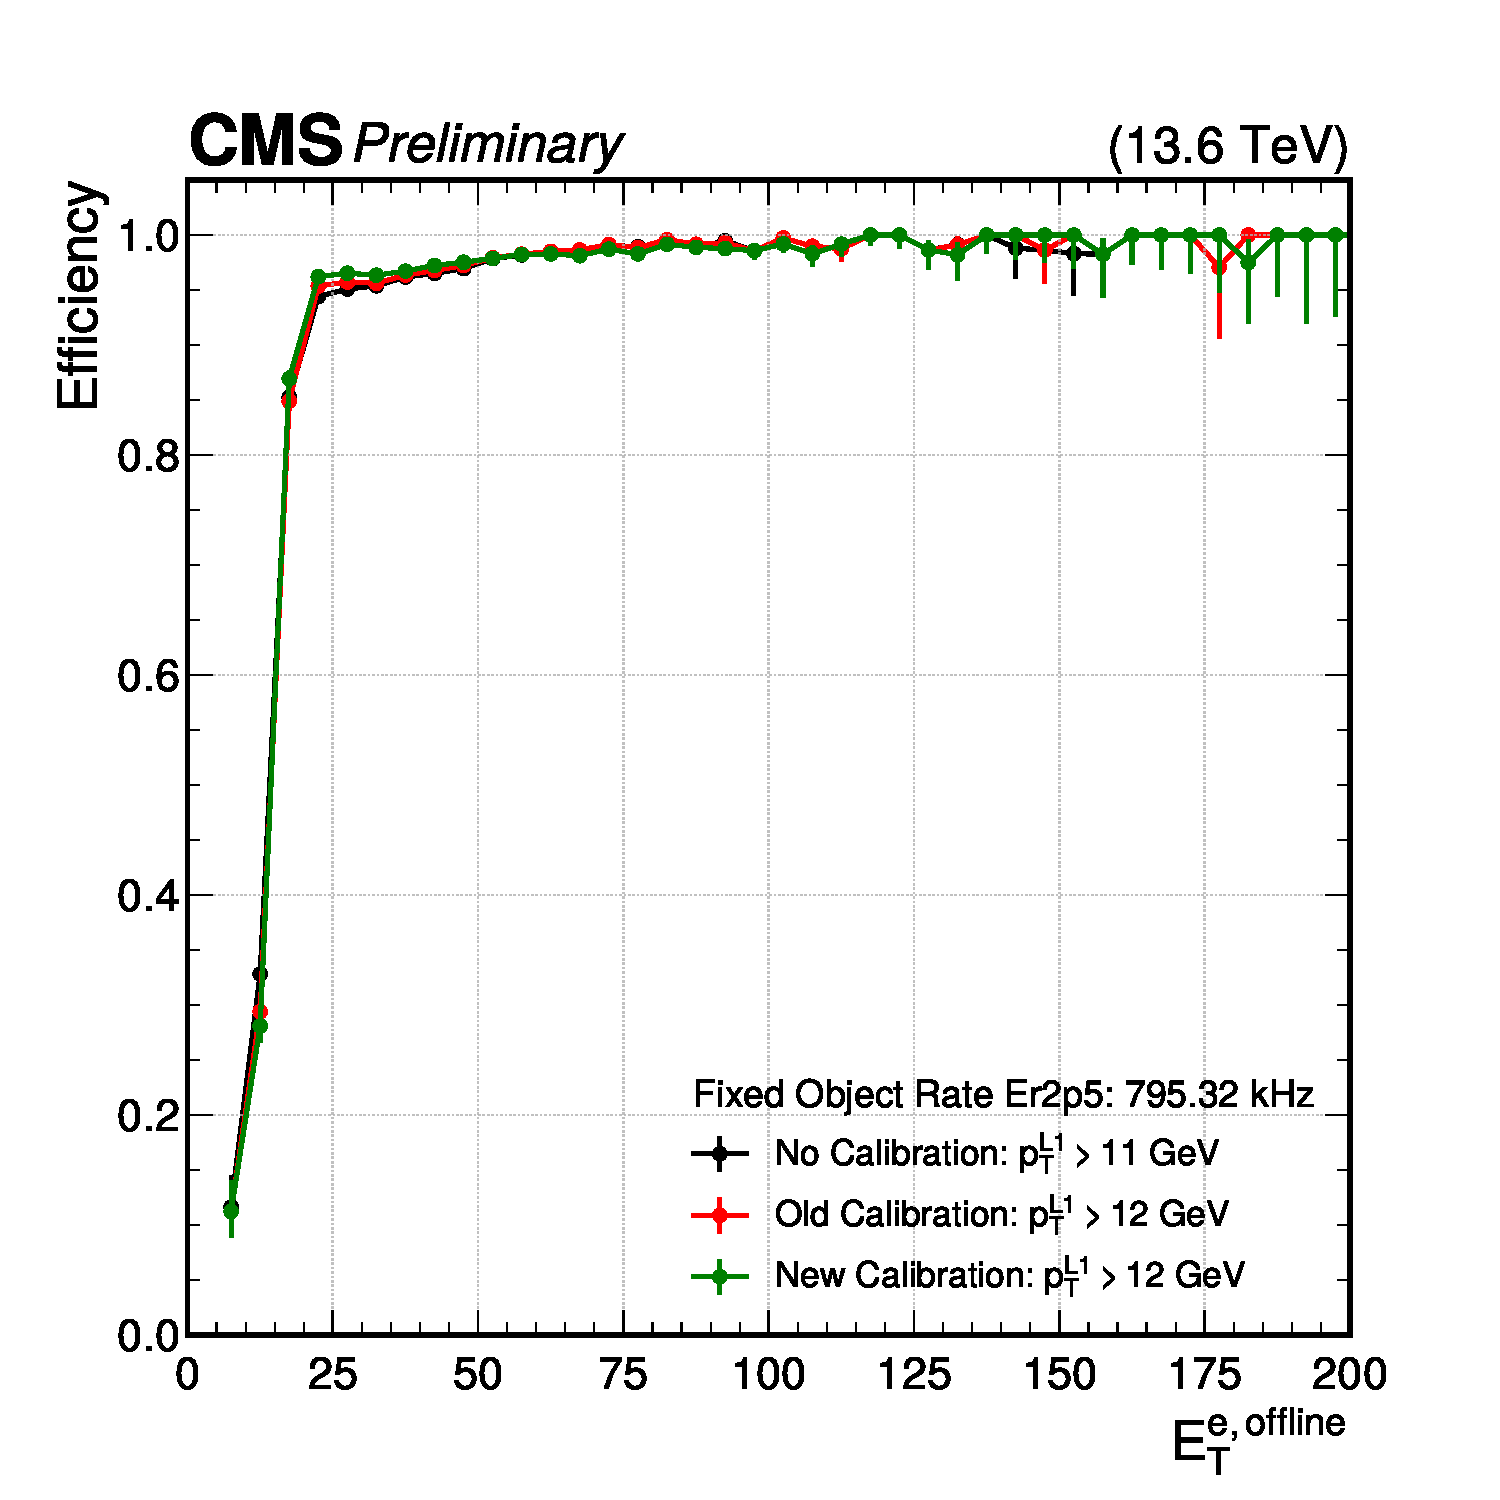
\includegraphics[width=0.5\linewidth]{Figures/L1TP/NN_Performance/turnon_fixedObjRateEr2p5_12__ele.pdf}}
    \subfloat[]{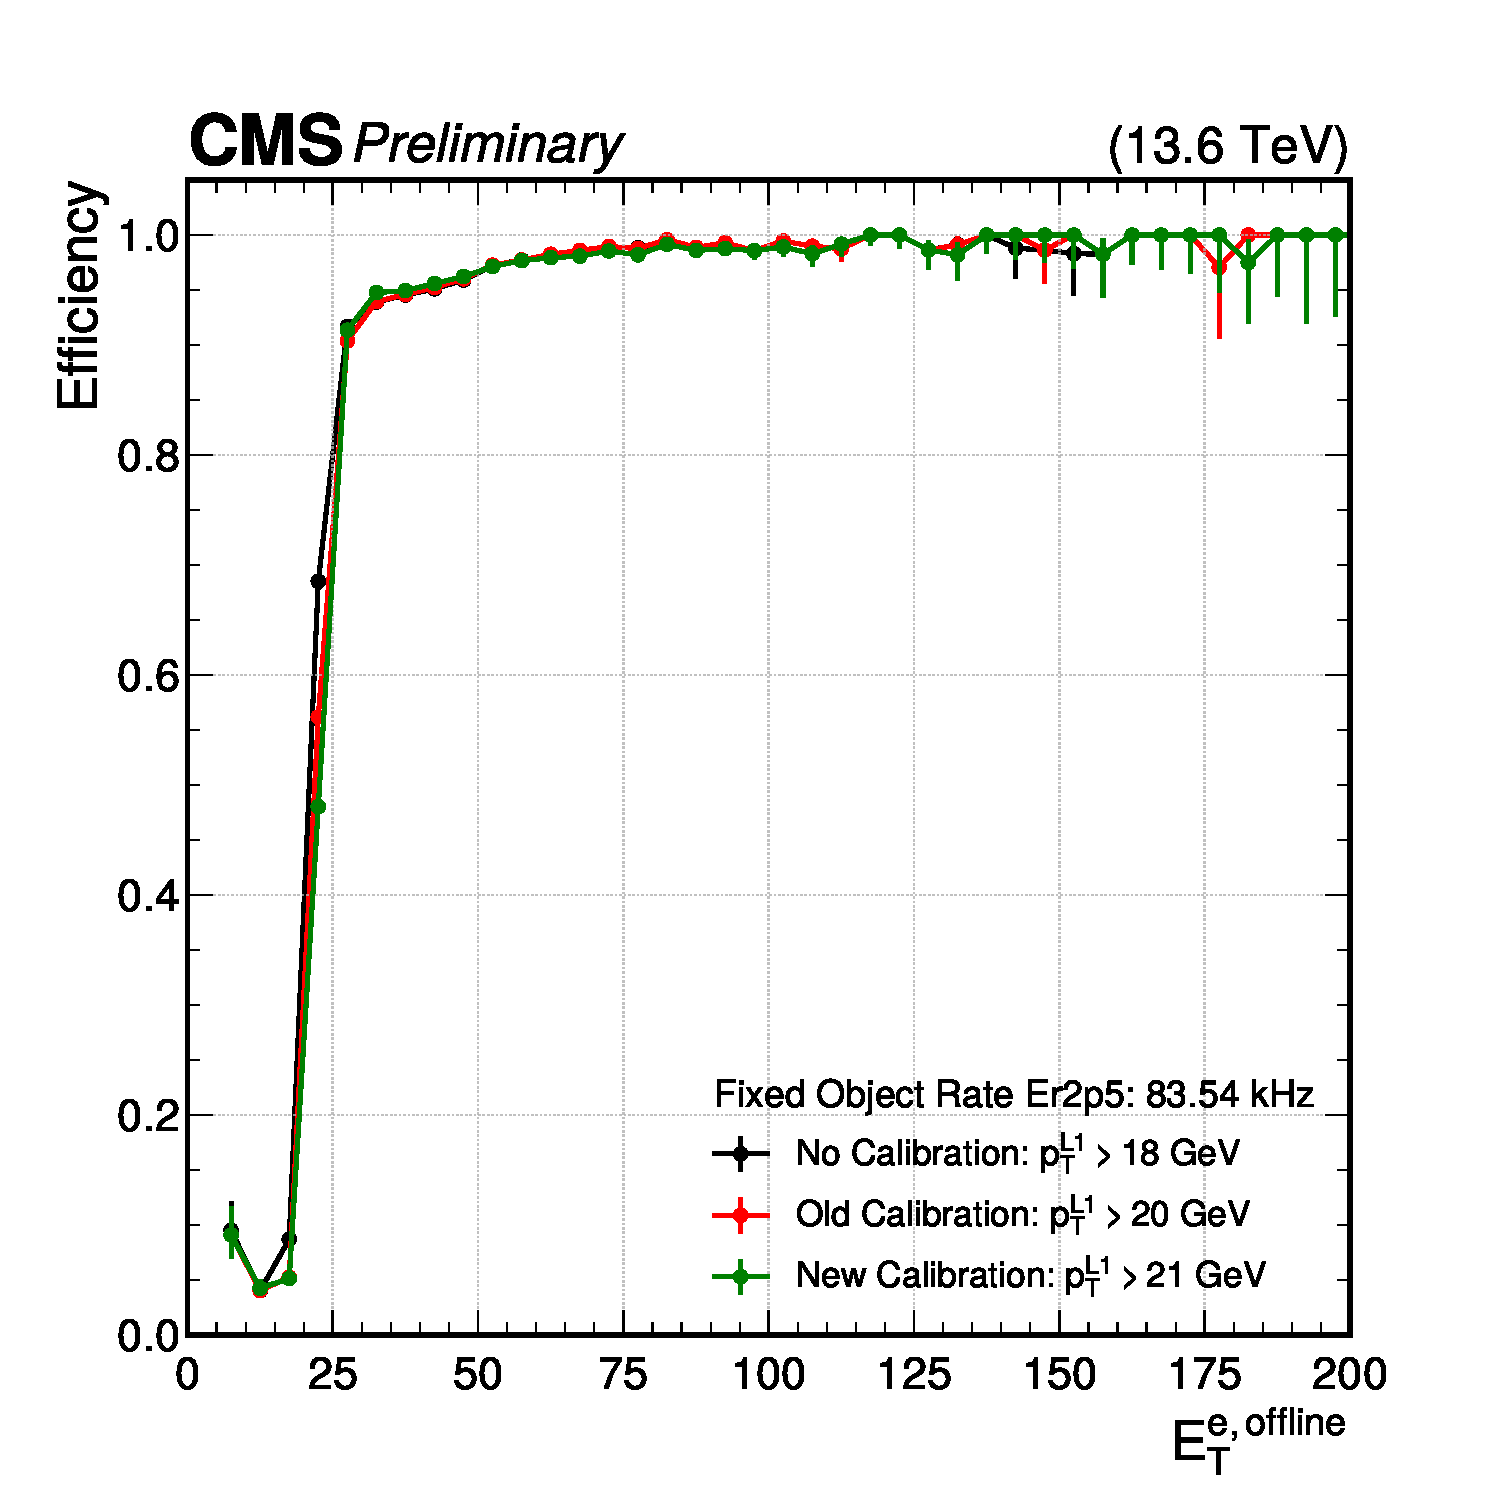
\includegraphics[width=0.5\linewidth]{Figures/L1TP/NN_Performance/turnon_fixedObjRateEr2p5_20__ele.pdf}}
    \caption{}
    \label{fig:NN_ECAL_TurnOn}
\end{figure}

\begin{figure}
    \centering
    \subfloat[]{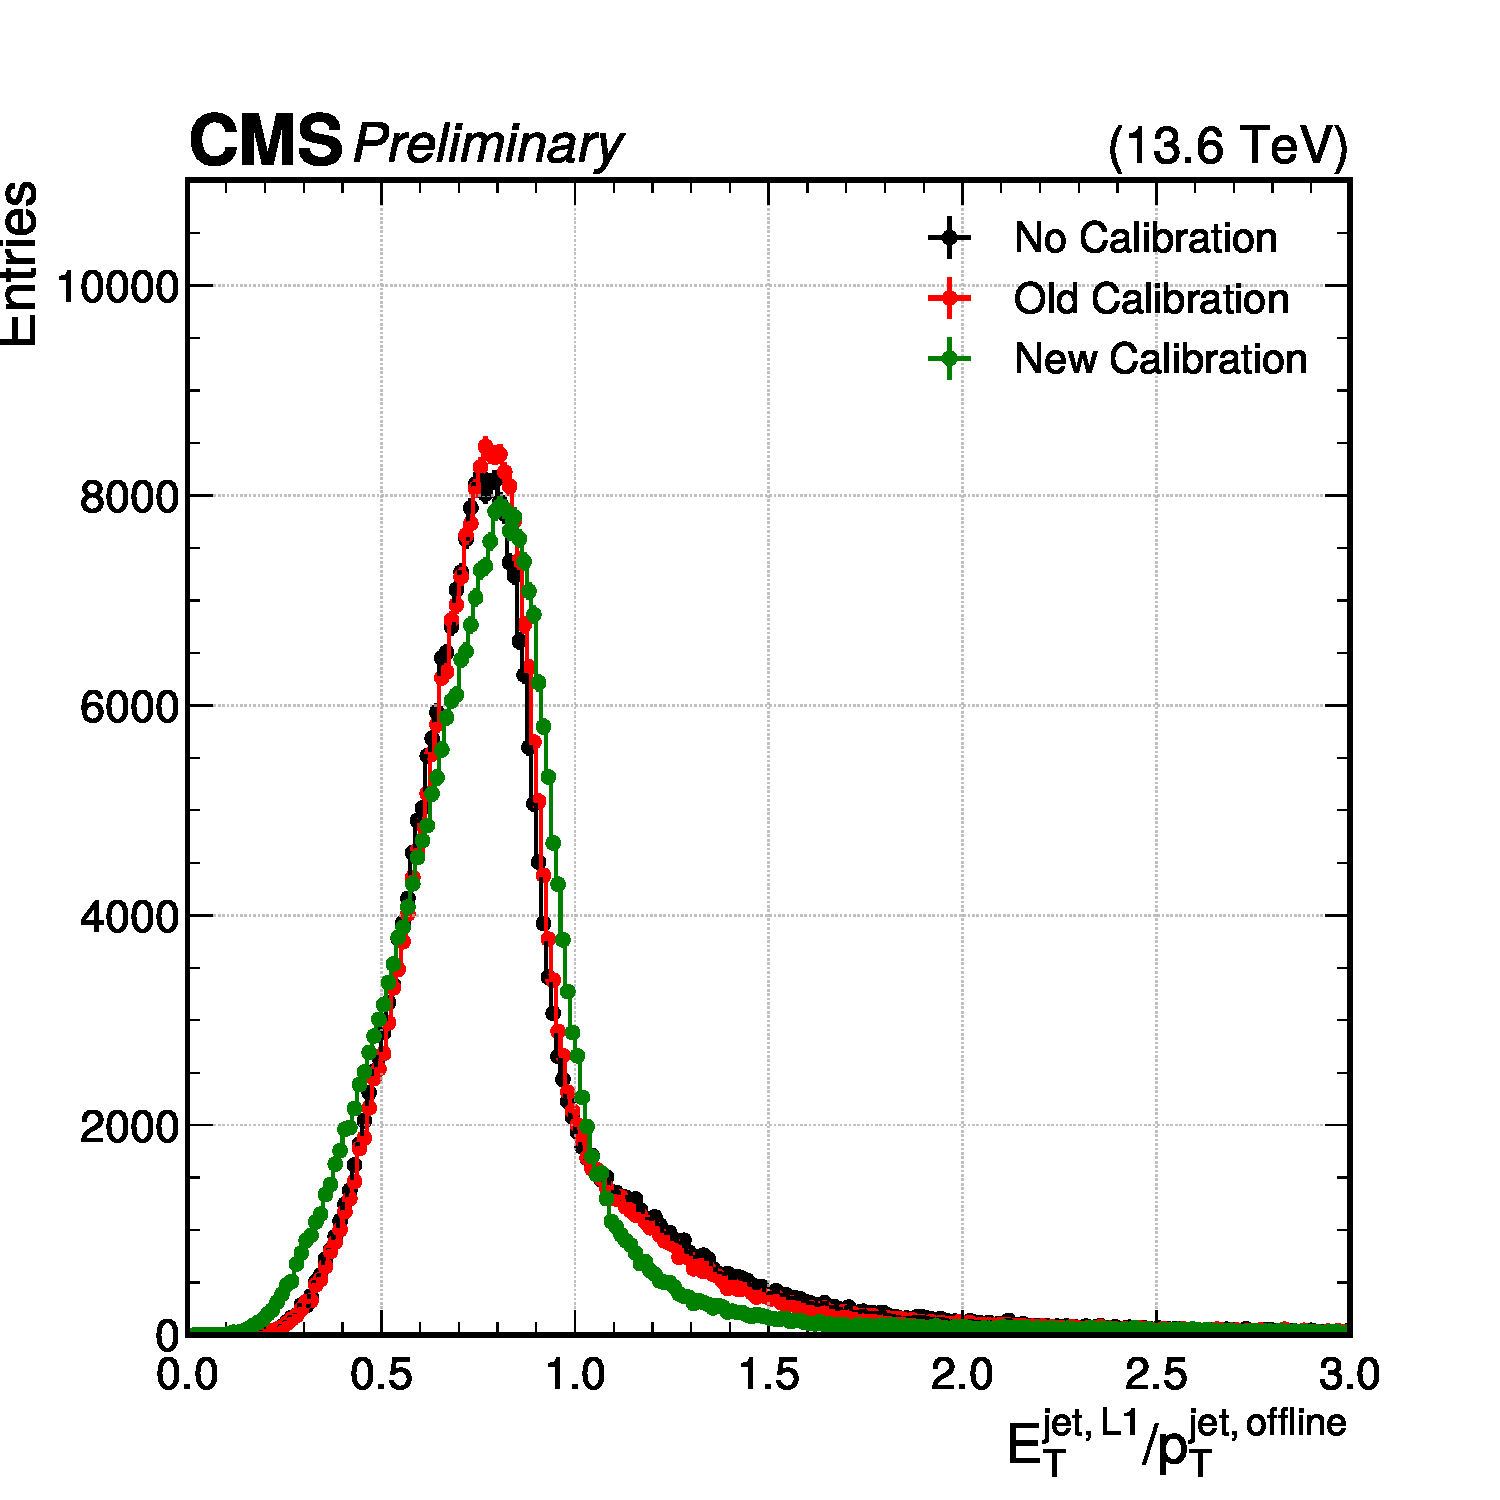
\includegraphics[width=0.5\linewidth]{Figures/L1TP/NN_Performance/response_inclusive__jet.pdf}}
    
    \subfloat[]{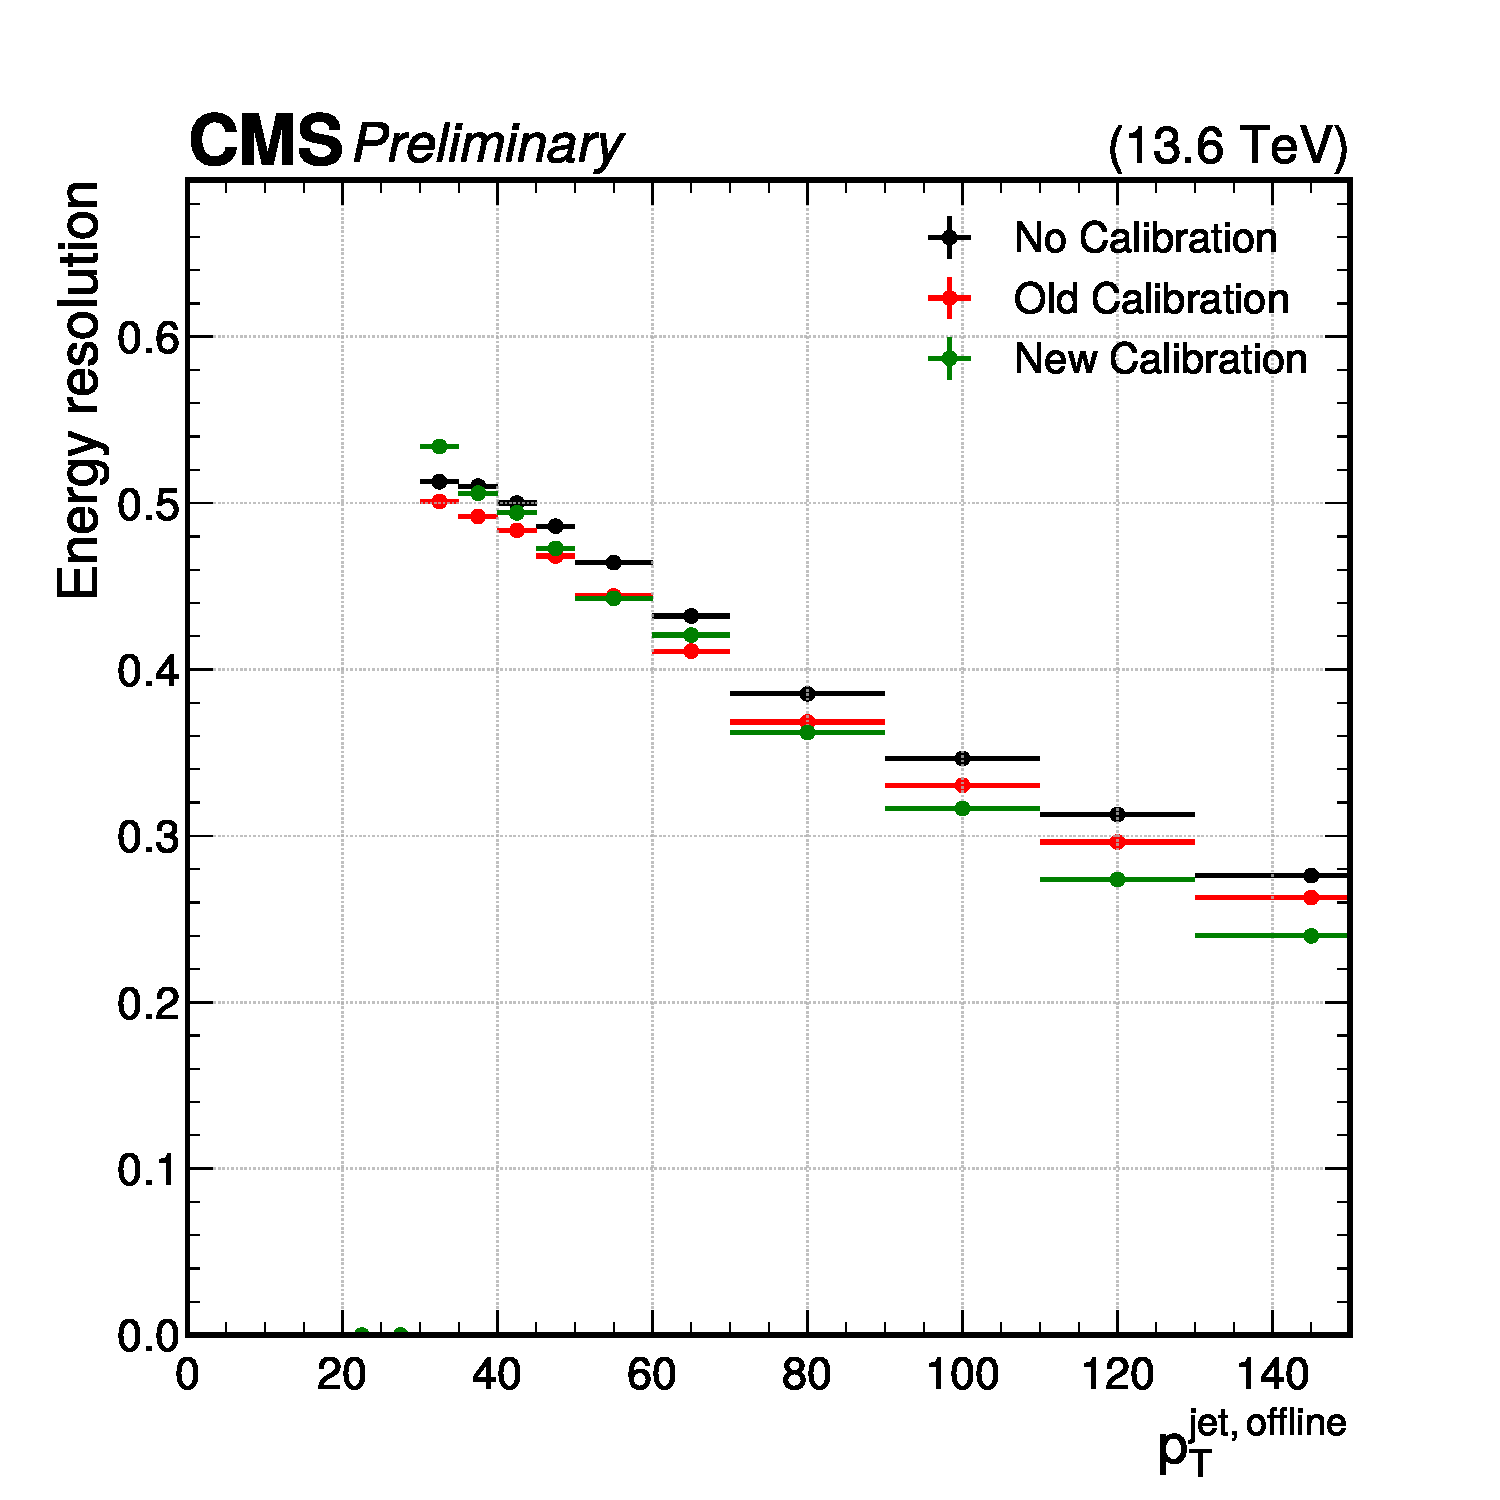
\includegraphics[width=0.5\linewidth]{Figures/L1TP/NN_Performance/resolution_ptBins__jet.pdf}}
    \subfloat[]{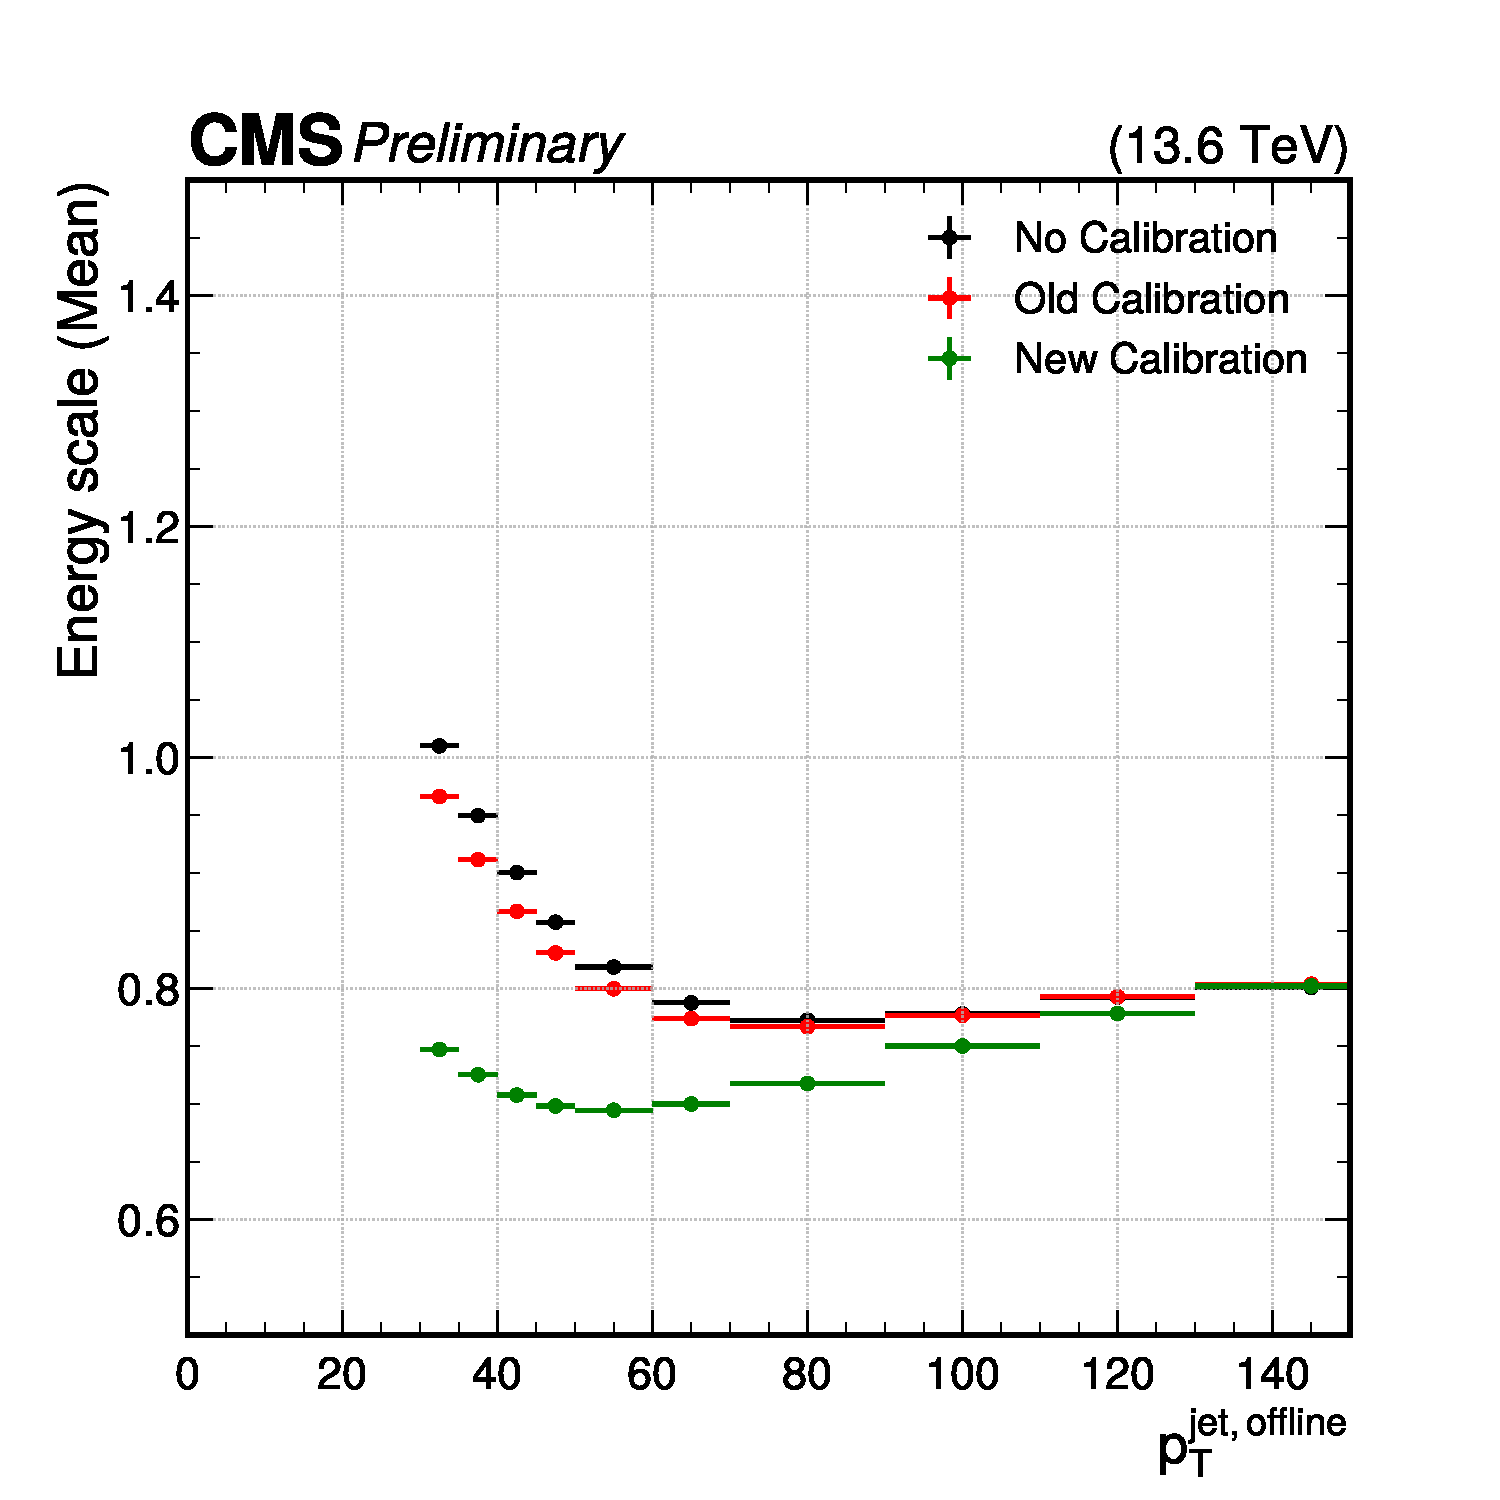
\includegraphics[width=0.5\linewidth]{Figures/L1TP/NN_Performance/scale_ptBins__jet.pdf}}
    \caption{}
    \label{fig:NN_HCAL_Response}
\end{figure}

\begin{figure}
    \centering
    \subfloat[]{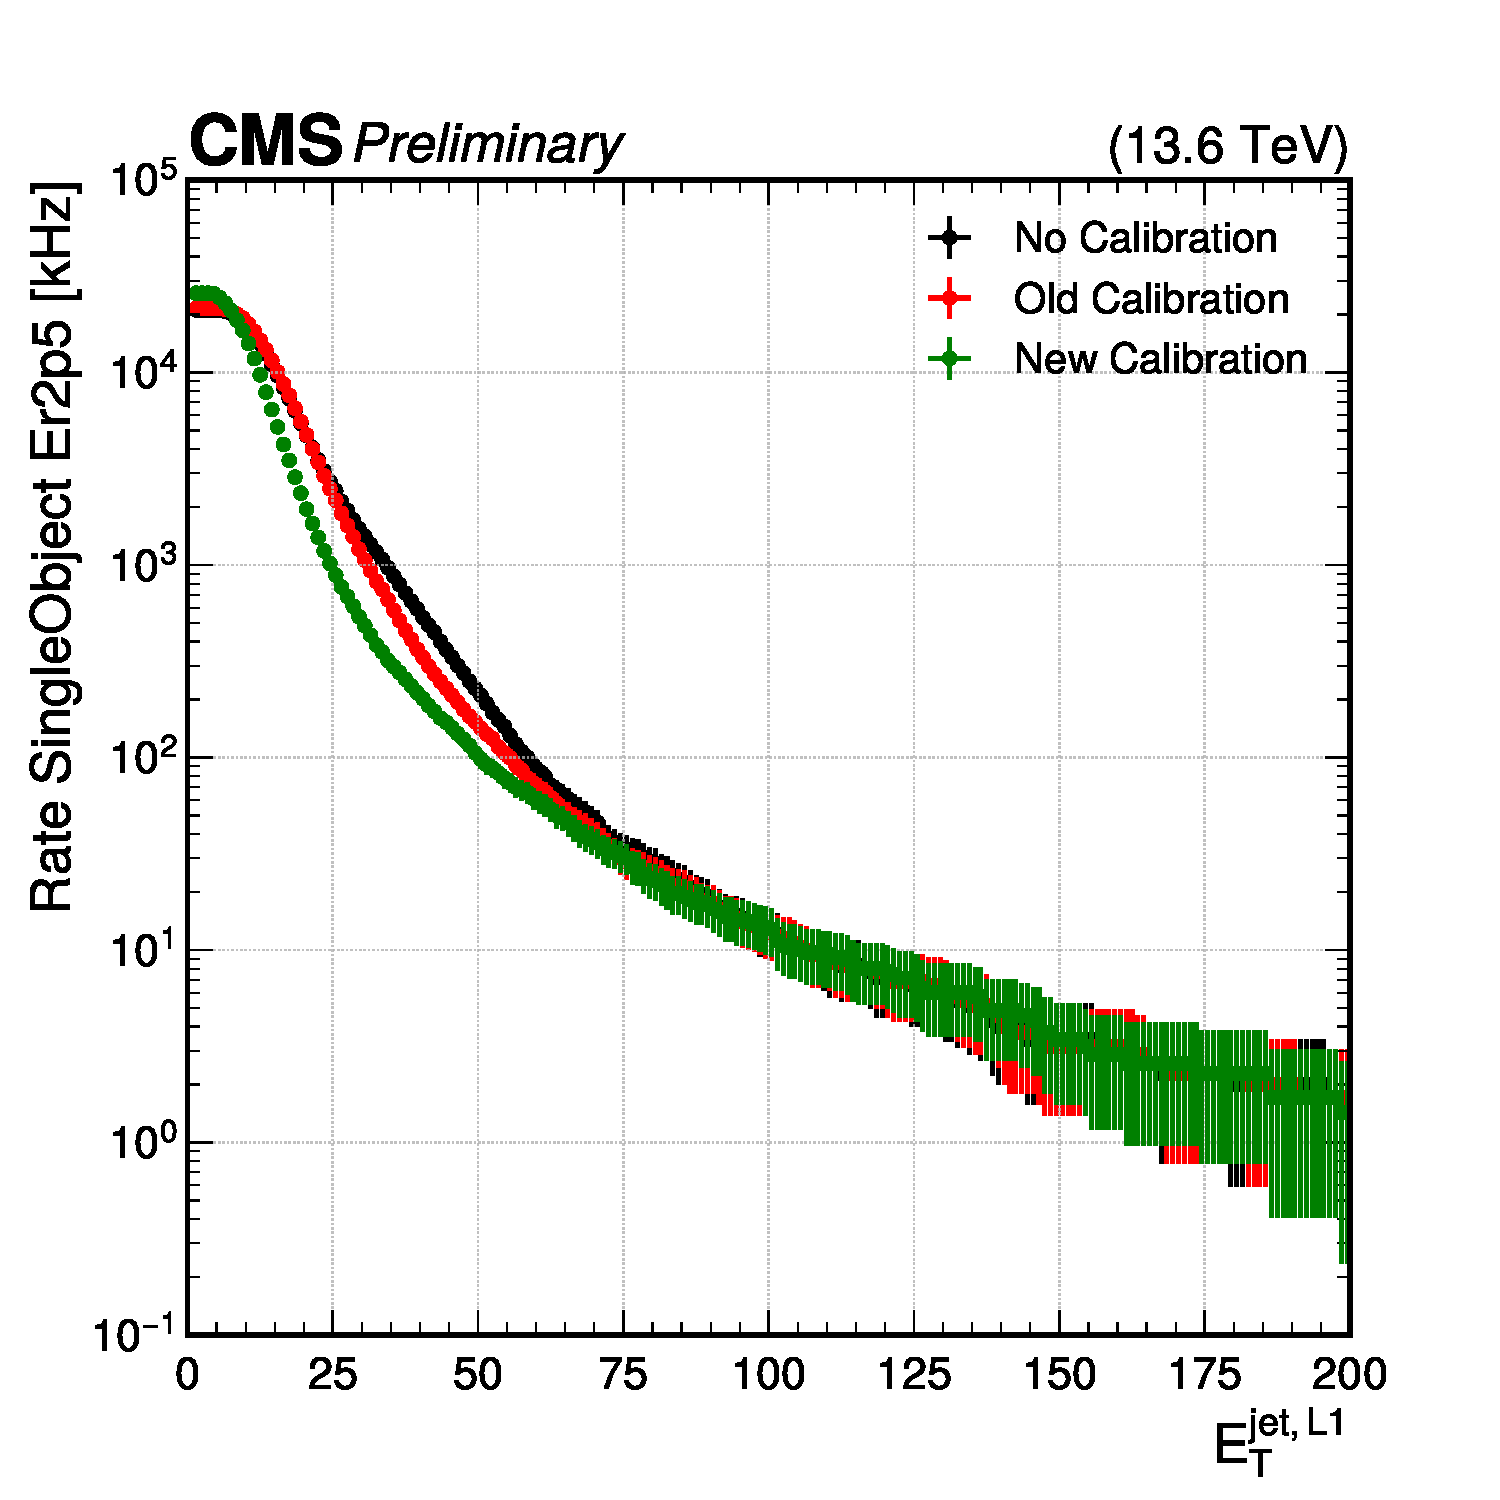
\includegraphics[width=0.5\linewidth]{Figures/L1TP/NN_Performance/rate_ObjEr2p5__jet.pdf}}
    
    \subfloat[]{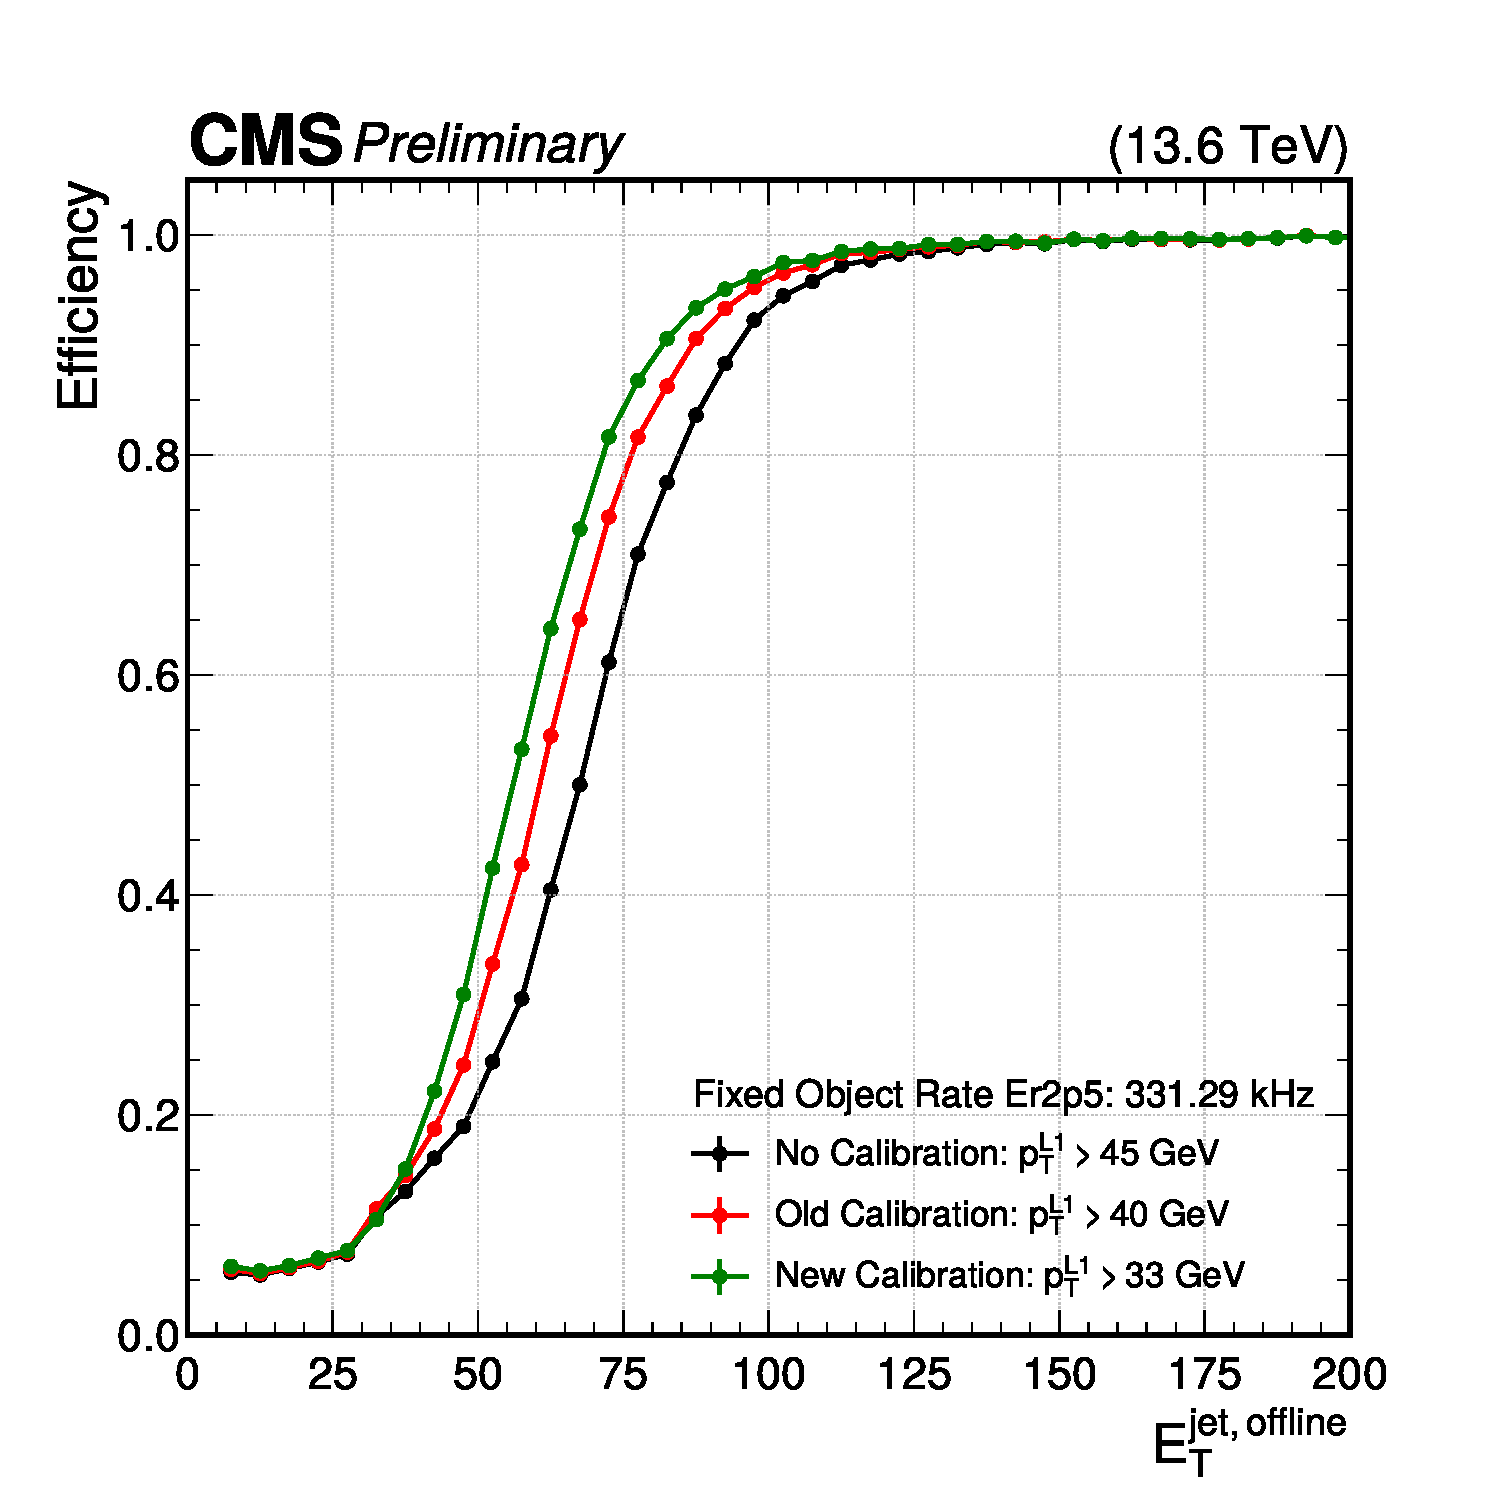
\includegraphics[width=0.5\linewidth]{Figures/L1TP/NN_Performance/turnon_fixedObjRateEr2p5_40__jet.pdf}}
    \subfloat[]{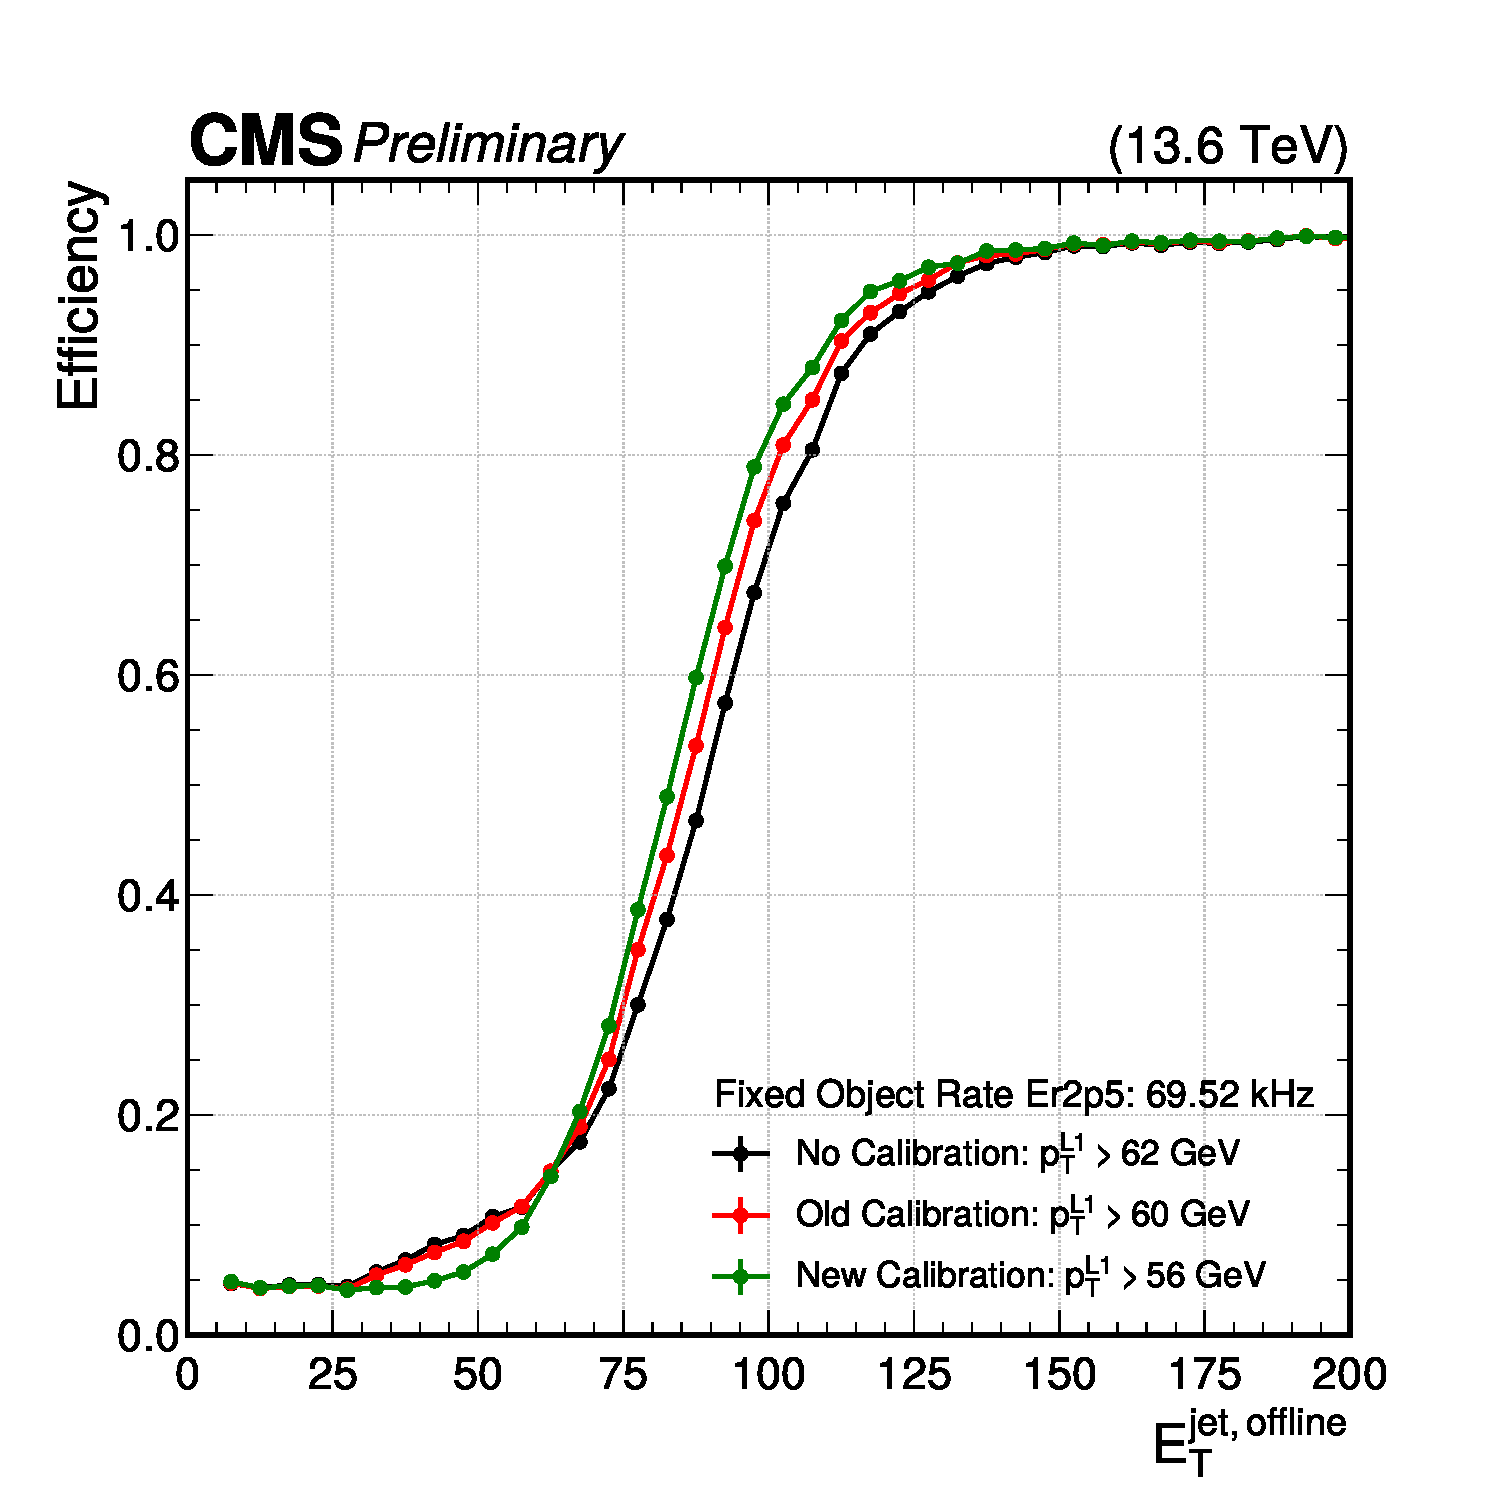
\includegraphics[width=0.5\linewidth]{Figures/L1TP/NN_Performance/turnon_fixedObjRateEr2p5_60__jet.pdf}}
    \caption{}
    \label{fig:NN_HCAL_TurnOn_ER2p5}
\end{figure}

\begin{figure}
    \centering
    \subfloat[]{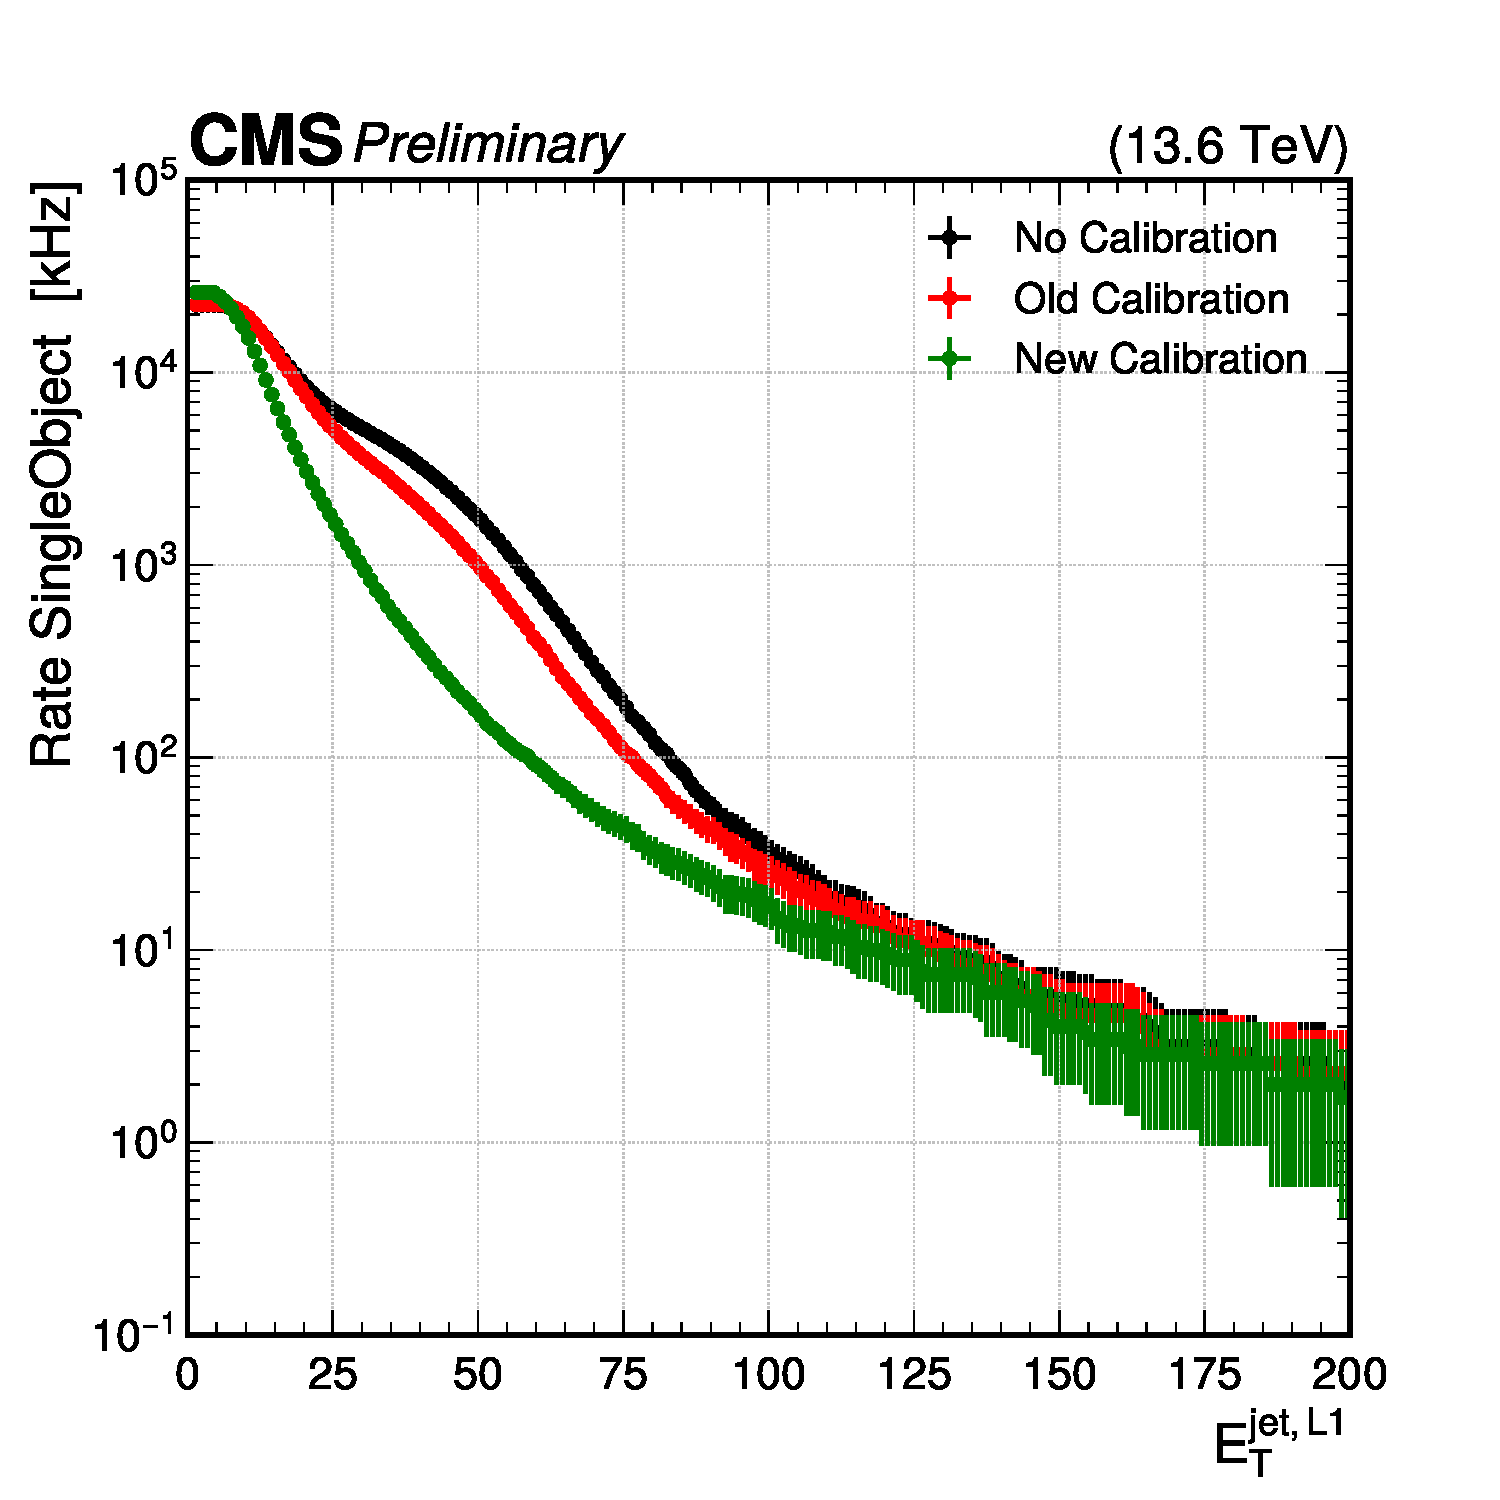
\includegraphics[width=0.5\linewidth]{Figures/L1TP/NN_Performance/rate_Obj__jet.pdf}}
    
    \subfloat[]{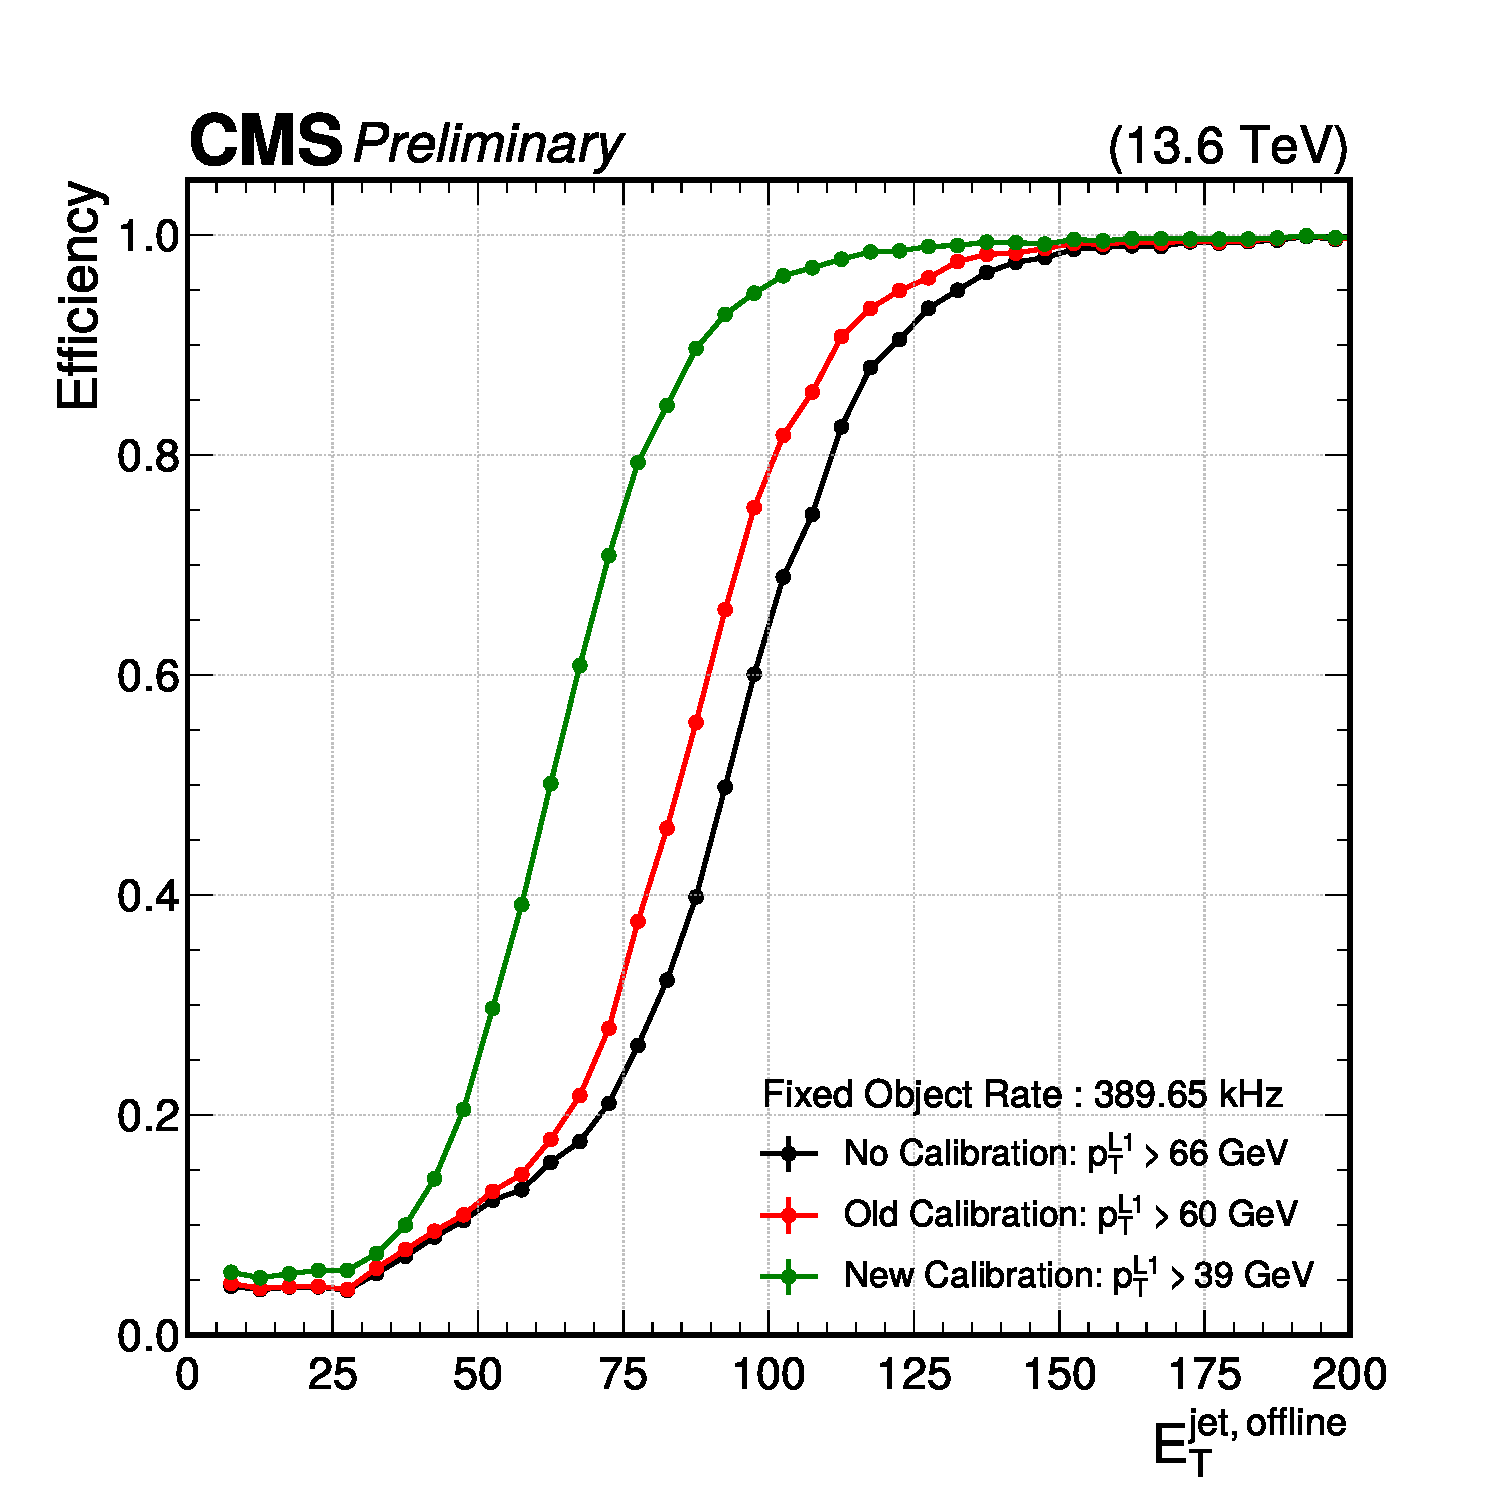
\includegraphics[width=0.5\linewidth]{Figures/L1TP/NN_Performance/turnon_fixedObjRate_60__jet.pdf}}
    \subfloat[]{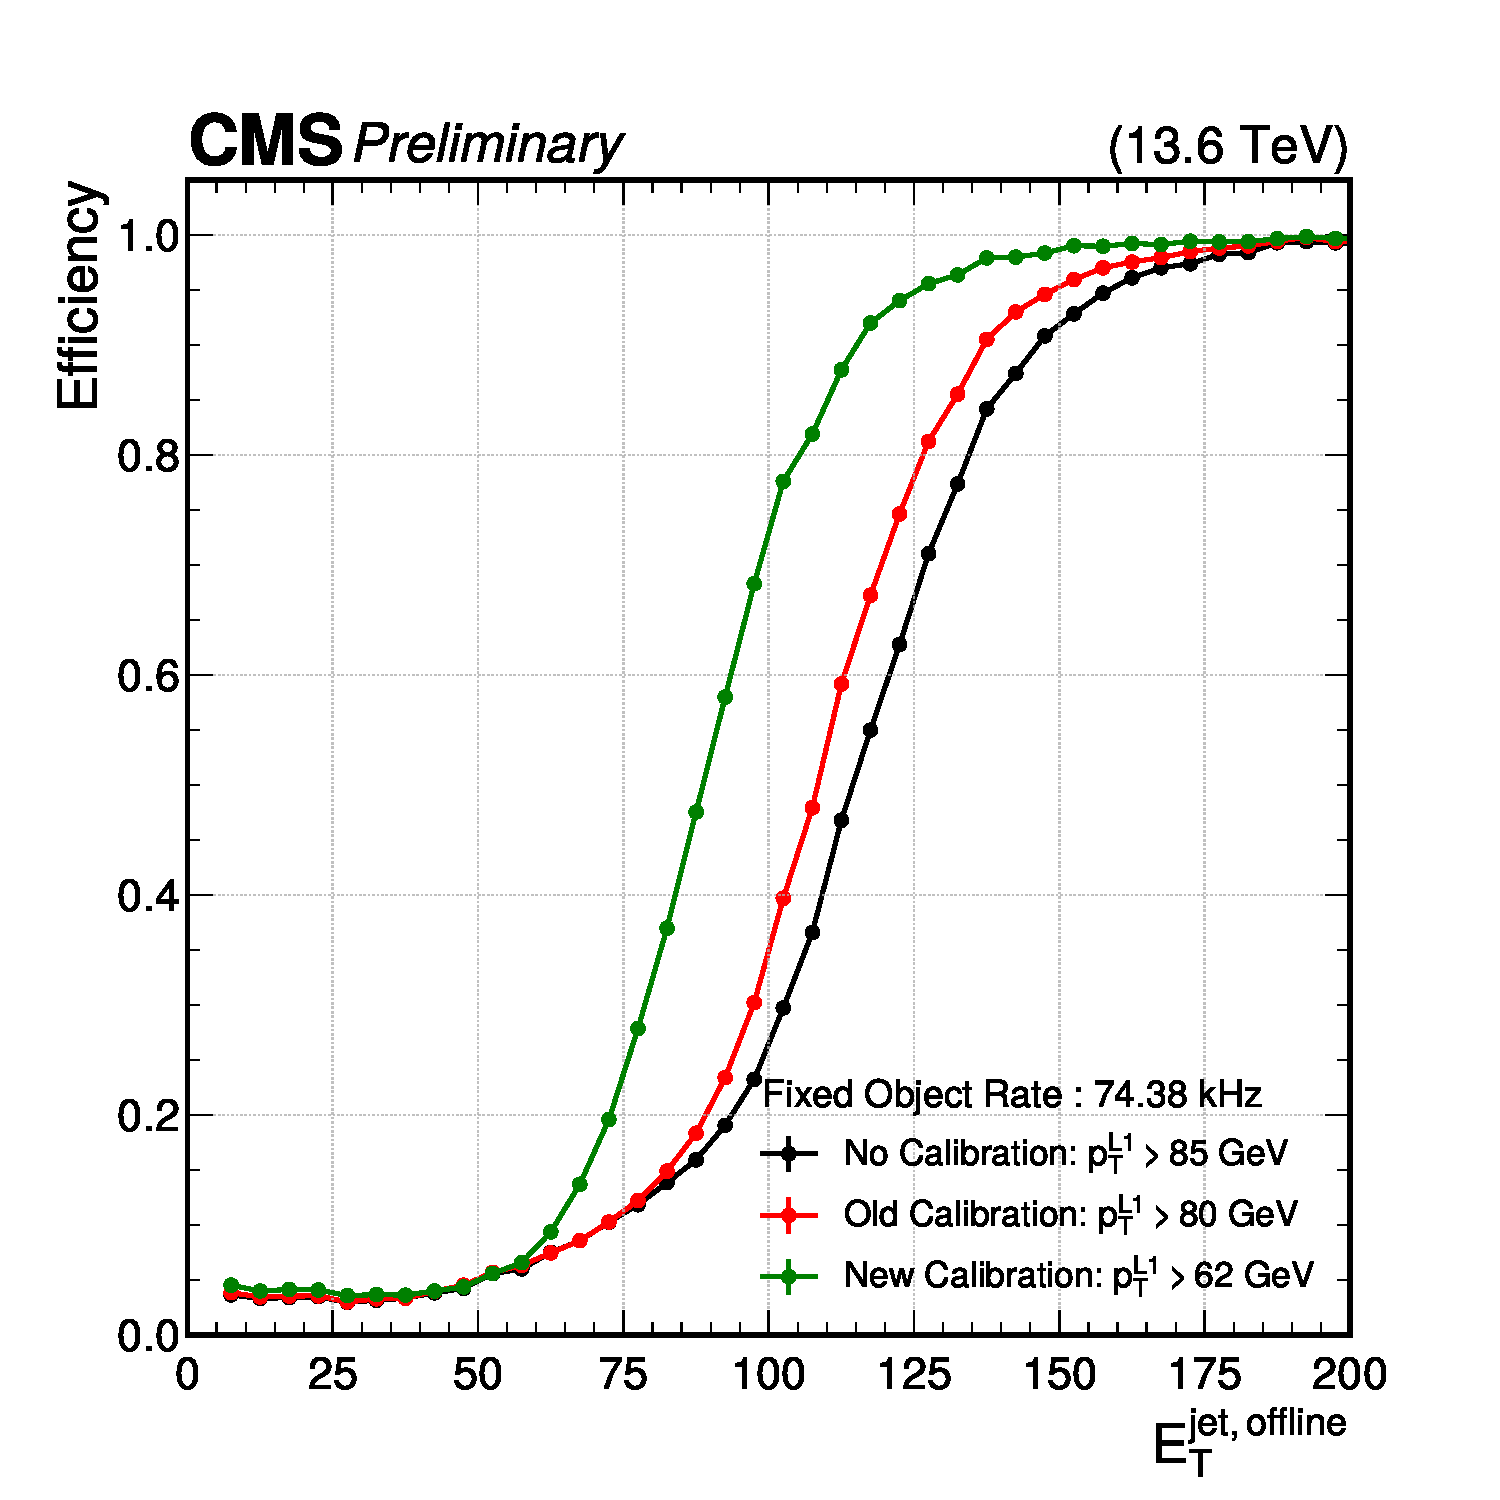
\includegraphics[width=0.5\linewidth]{Figures/L1TP/NN_Performance/turnon_fixedObjRate_80__jet.pdf}}
    \caption{}
    \label{fig:NN_HCAL_TurnOn}
\end{figure}

The ECAL performance is shown in terms of inclusive response, resolution and scale in Figure~\ref{fig:NN_ECAL_Response}. The new NN approach provides a narrower, better centred distribution of the L1 energy response for $e/\gamma$, the resolution is consistently improved across the majority of the $p_T$ range, and the scale is closer to unity. The corresponding Layer-1 expected rate, so as the efficiency turn-on curves for two exemplary fixed rate values are represented in Figure~\ref{fig:NN_ECAL_TurnOn}: the new calibration ensured sharper turn-on curves compared to the old calibration in the low $p_T$ range, while the performance is comparable, or slightly reduced, in the high $p_T$ range.

The HCAL performance of the new NN approach is compared to the other configurations in Figure~\ref{fig:NN_HCAL_Response}, in terms of L1 jet energy response, resolution and scale. The distribution of the response shows comparable performance of the new NN-based scale factors with respect to the other methods: the right tail at higher response is reduced, however there is no significant improvement in terms of resolution or scale. In particular, the reduced scale is driven by the rate term in the loss function, whose relative importance has been optimised in order to provide the optimal efficiency turn-on curve. Figures~\ref{fig:NN_HCAL_TurnOn_ER2p5} and \ref{fig:NN_HCAL_TurnOn} show a performance comparison of the three configurations in terms of rate and efficiency turn-on curves for the inclusive detector response and for the restricted case of $|\eta|<2.5$, where the latter is of particular interest for the L1 trigger performance since a vast number of trigger seeds only consider this pseudorapidity region, less affected by the pile-up activity.
The efficiency turn-on curves show an impressive improvement coming from the NN approach, with reduced rate and better centred turn-on curves: this result is mainly driven by the impact of the new calibration factors on the rate rather than an improvement on the resolution, which is comparable to the old method.

\subsection{Limitations of the Neural Network approach} % 30/6 - morning
% model interpretability
% customisability

The performance presented for the NN approach are the result of a careful optimisation of the NN hyper-parameters, conducted by scanning different values for the loss parameters and for the definition of the network architecture. Figure~\ref{fig:NN_HyperParameters} shows the effect of different values of the parameters $C$ and $D$ in the loss function, 

\begin{figure}
    \centering
    \subfloat[]{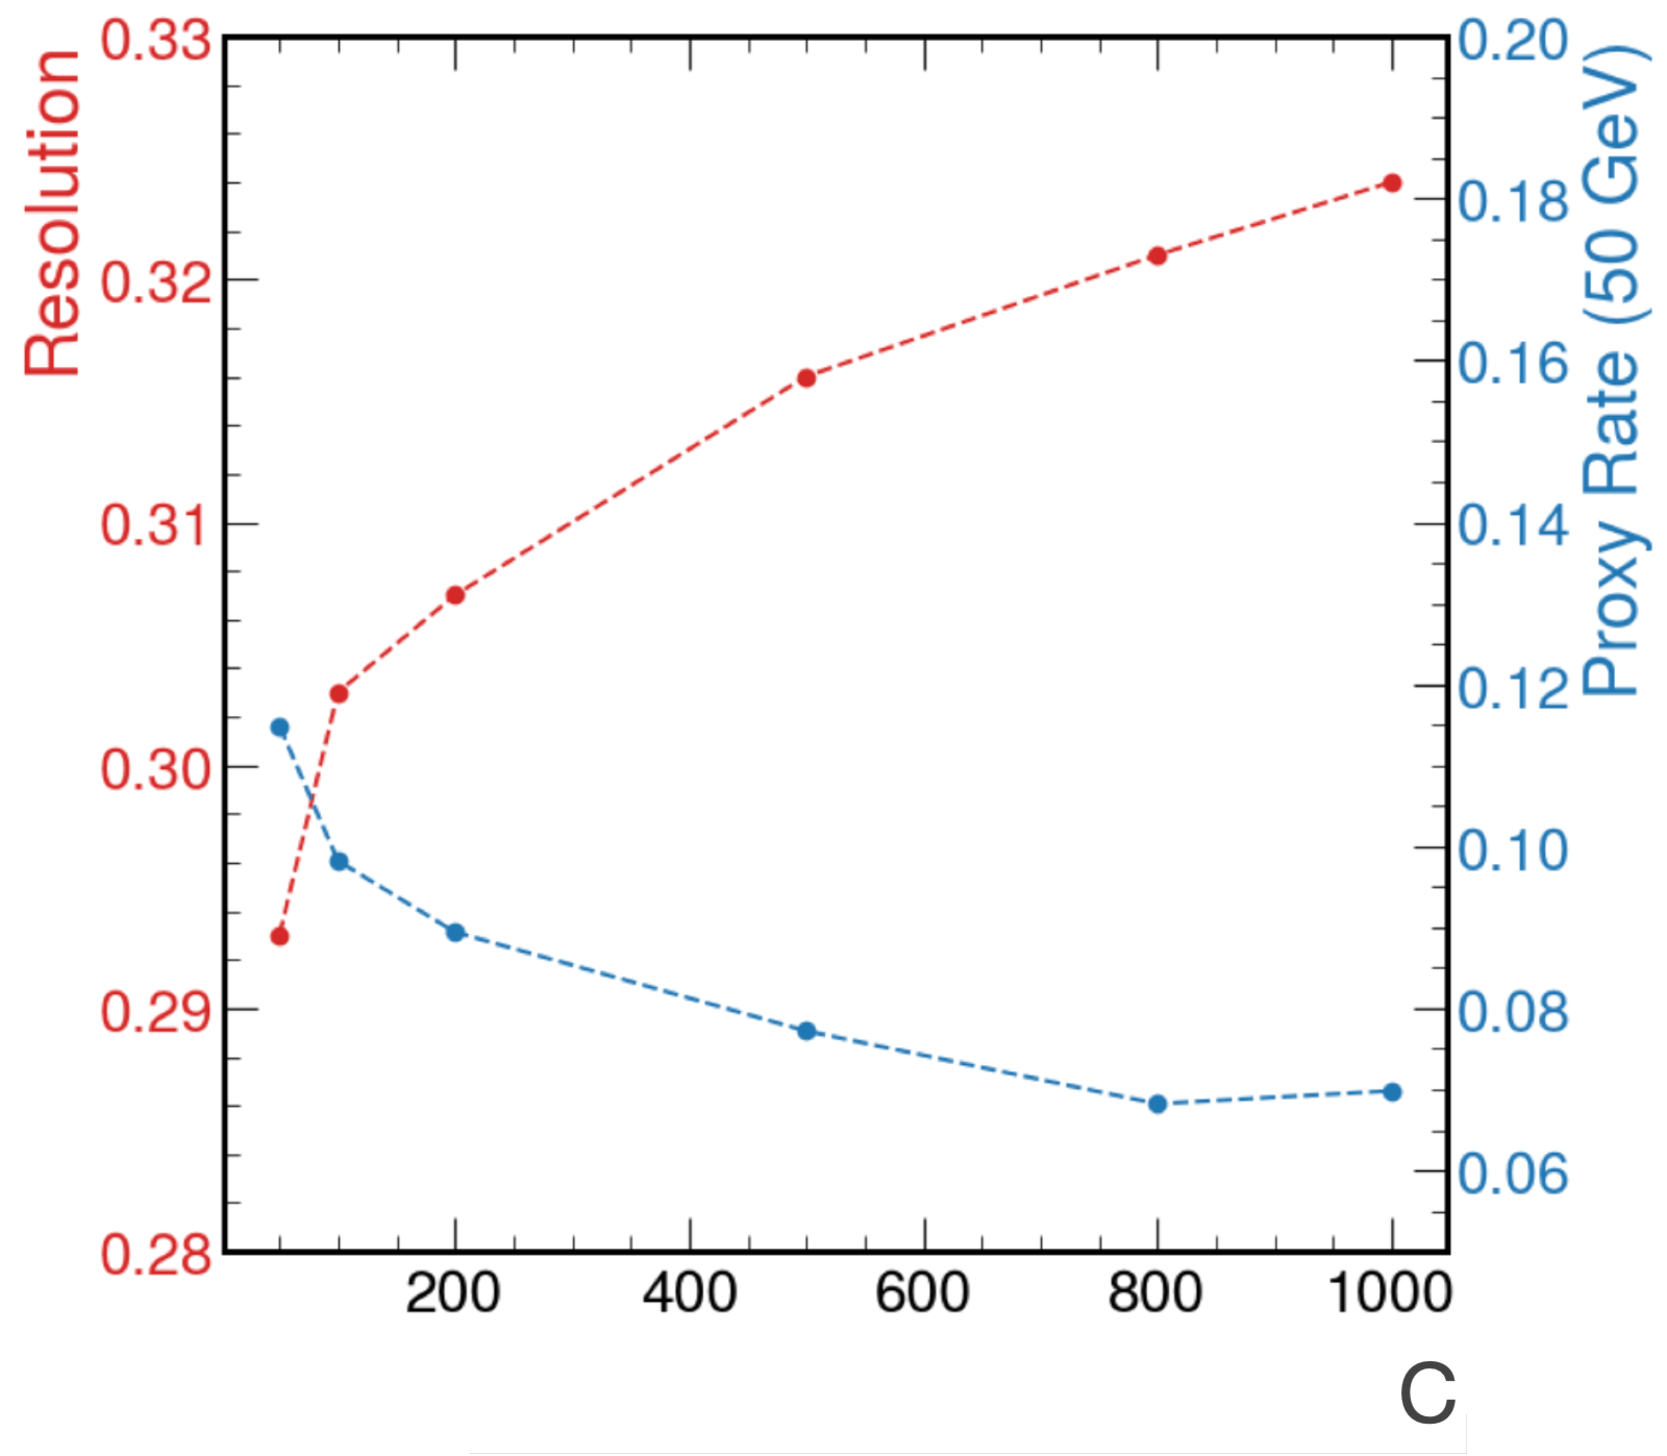
\includegraphics[width=0.4\linewidth]{Figures/L1TP/NN_ParameterC.pdf}}
    \hspace{1cm}
    \subfloat[]{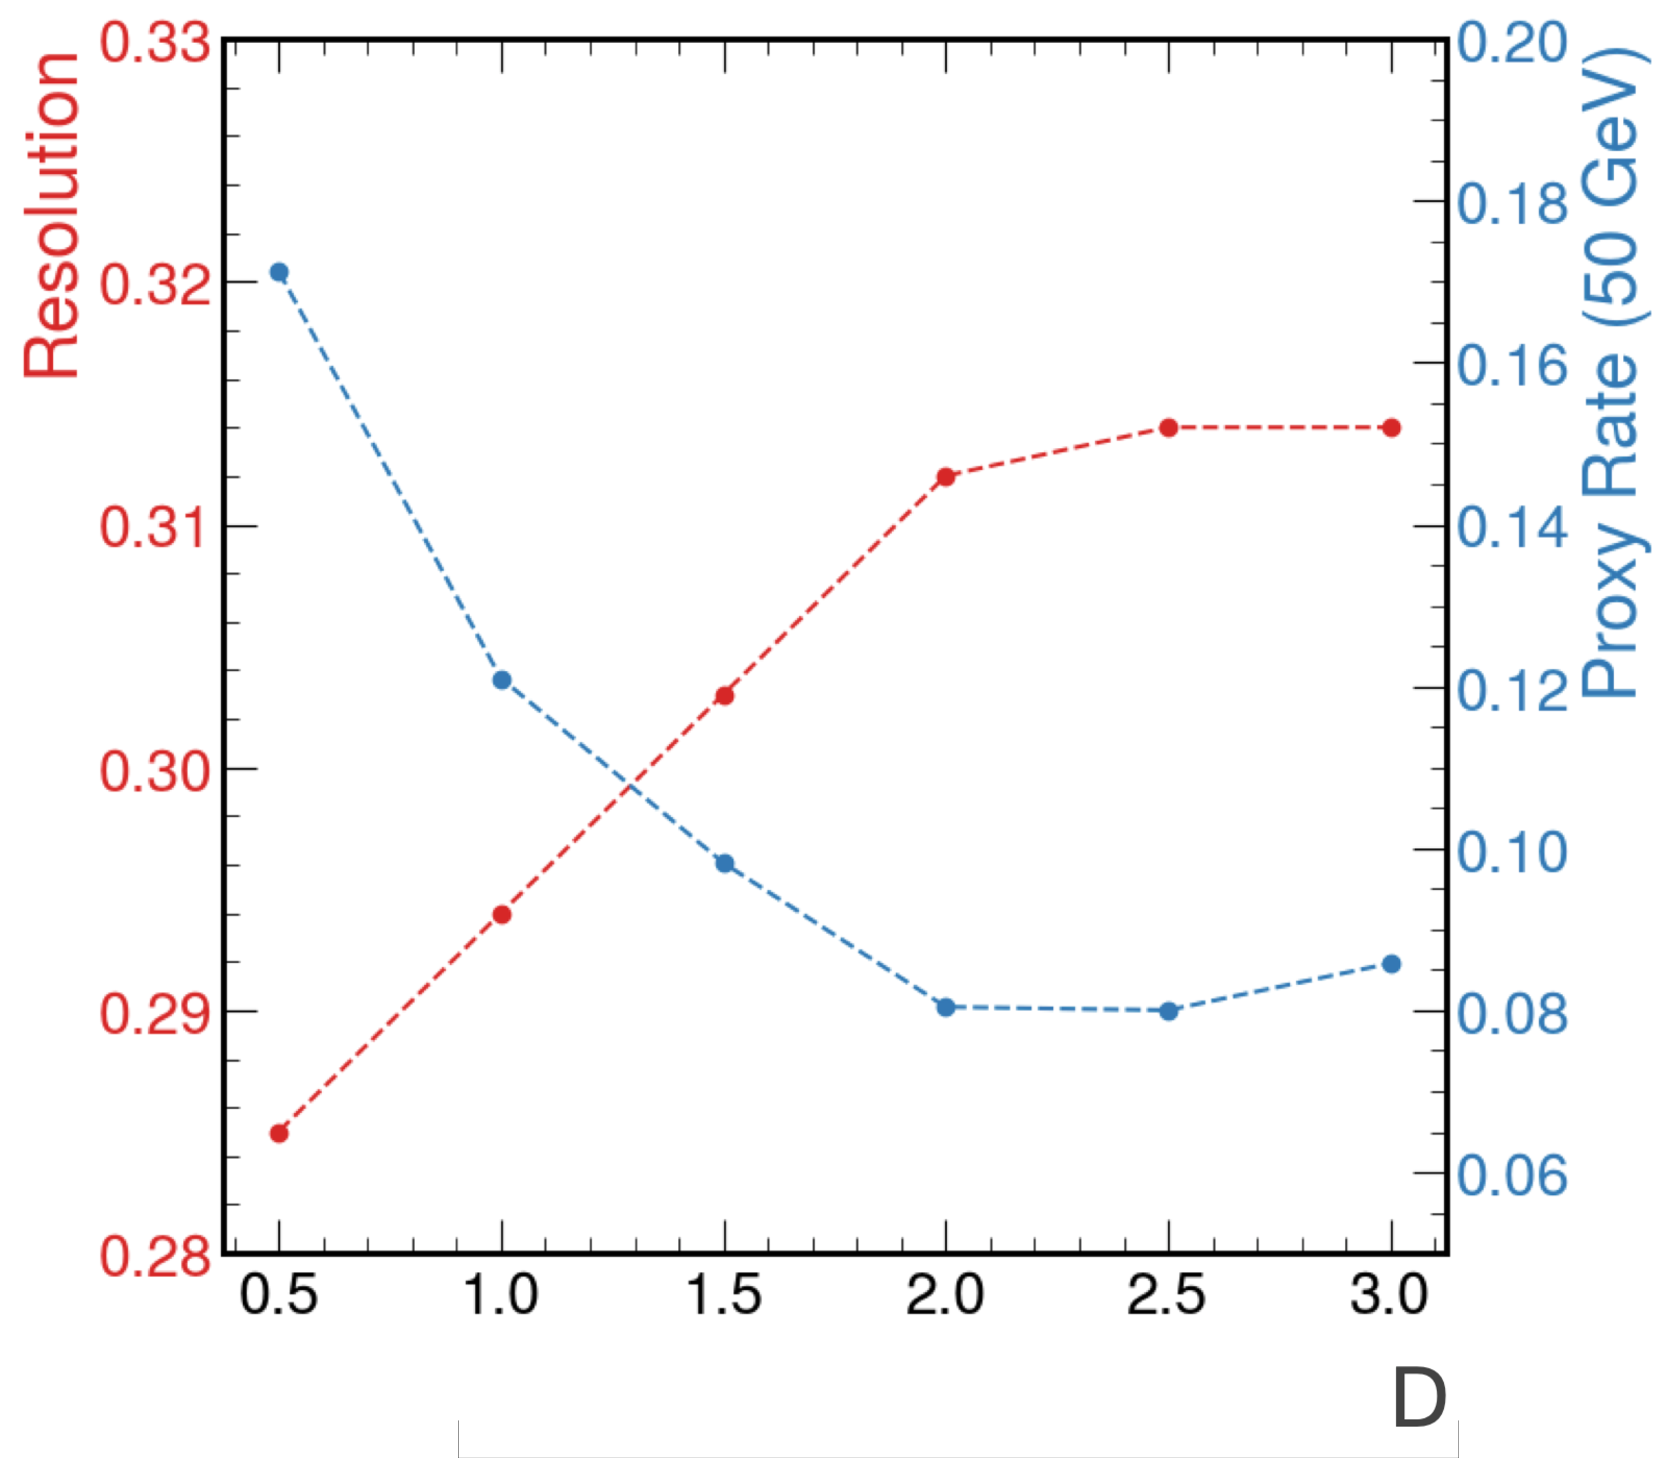
\includegraphics[width=0.4\linewidth]{Figures/L1TP/NN_ParameterD.pdf}}
    \caption{}
    \label{fig:NN_HyperParameters}
\end{figure}

\newpage

\section{The differentiable programming approach} % 30/6 - afternoon
% \subsection{A discrete approach} 
\subsection{Input dataset and optimisation} % 30/6 - afternoon


\subsection{Calibration factors and performance} % 30/6 - night

\begin{figure}
    \centering
    \subfloat[]{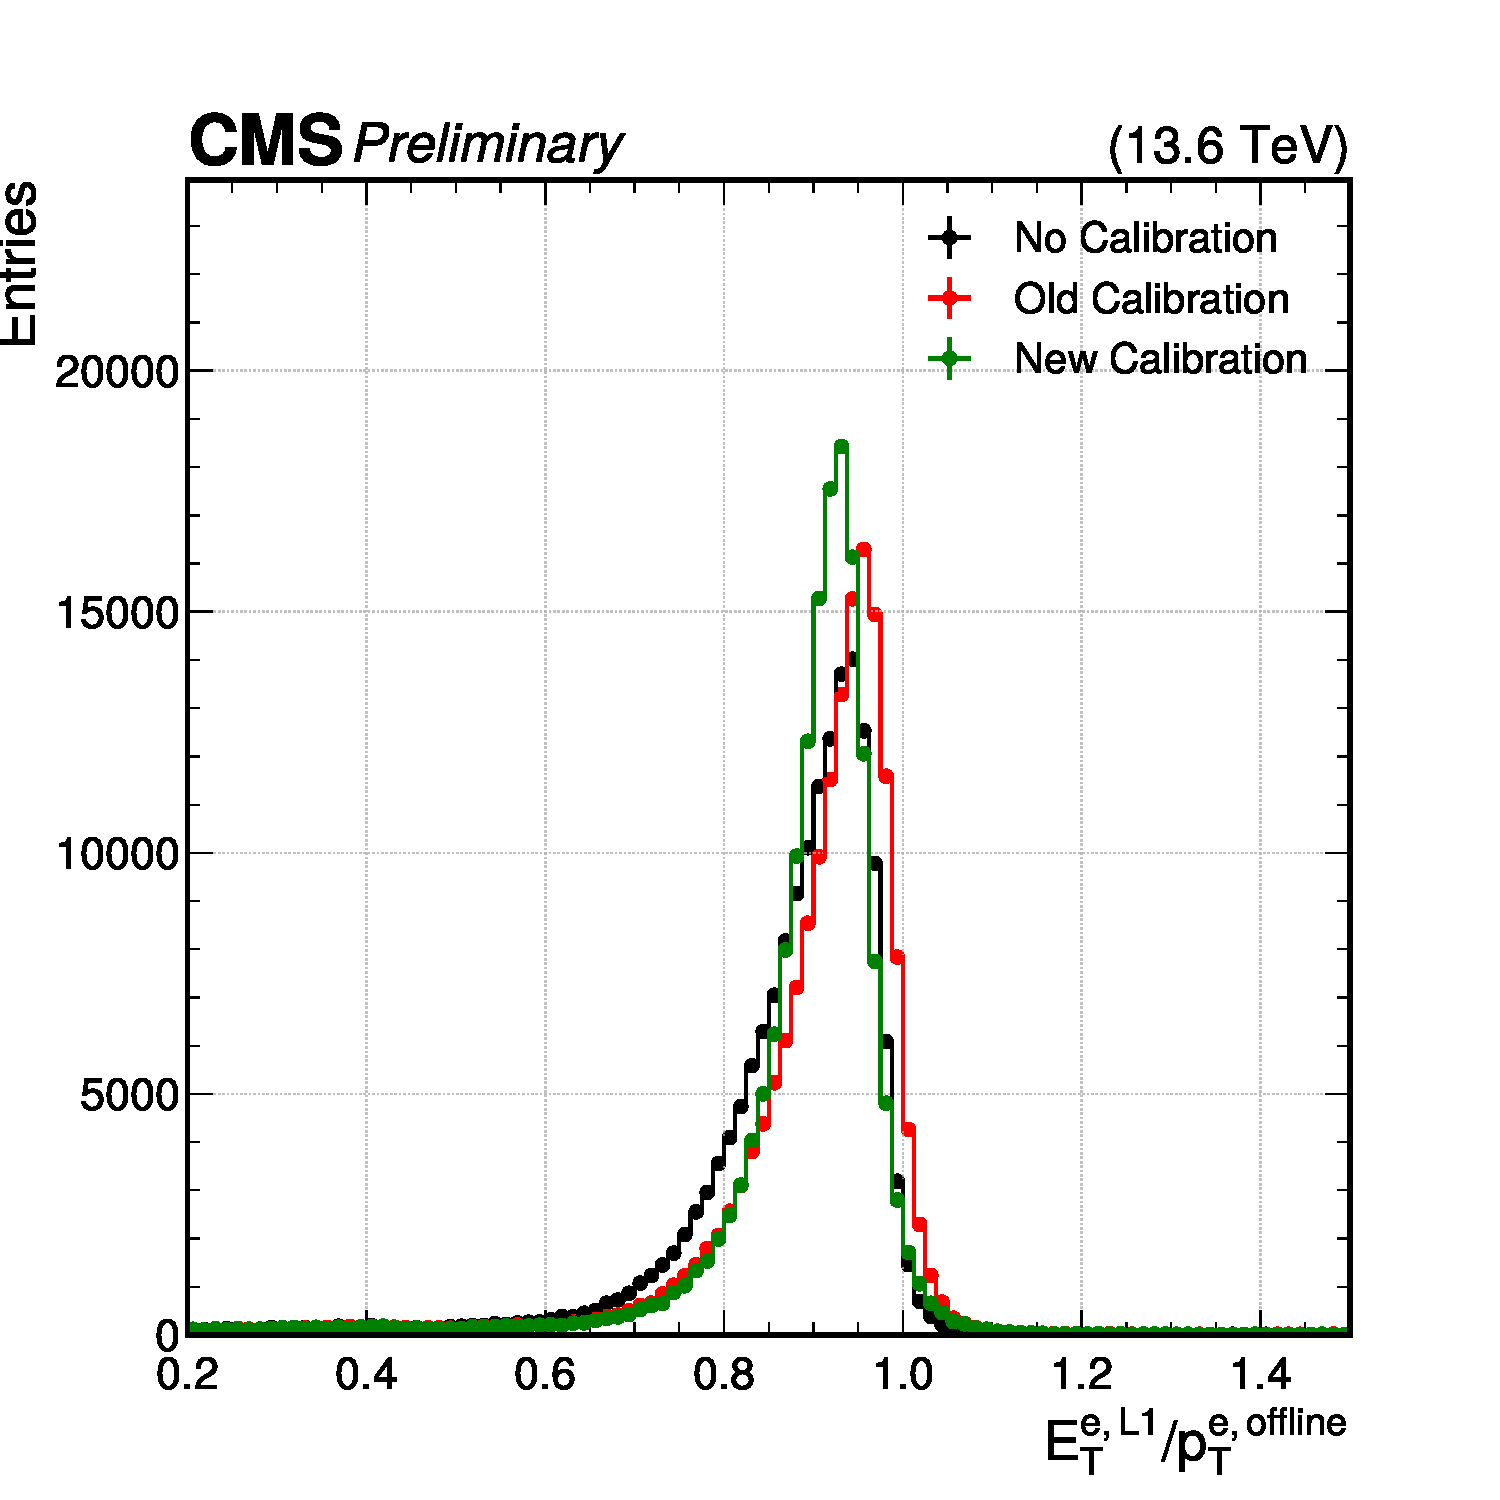
\includegraphics[width=0.5\linewidth]{Figures/L1TP/JAX_Performance/response_inclusive__ele.pdf}}
    
    \subfloat[]{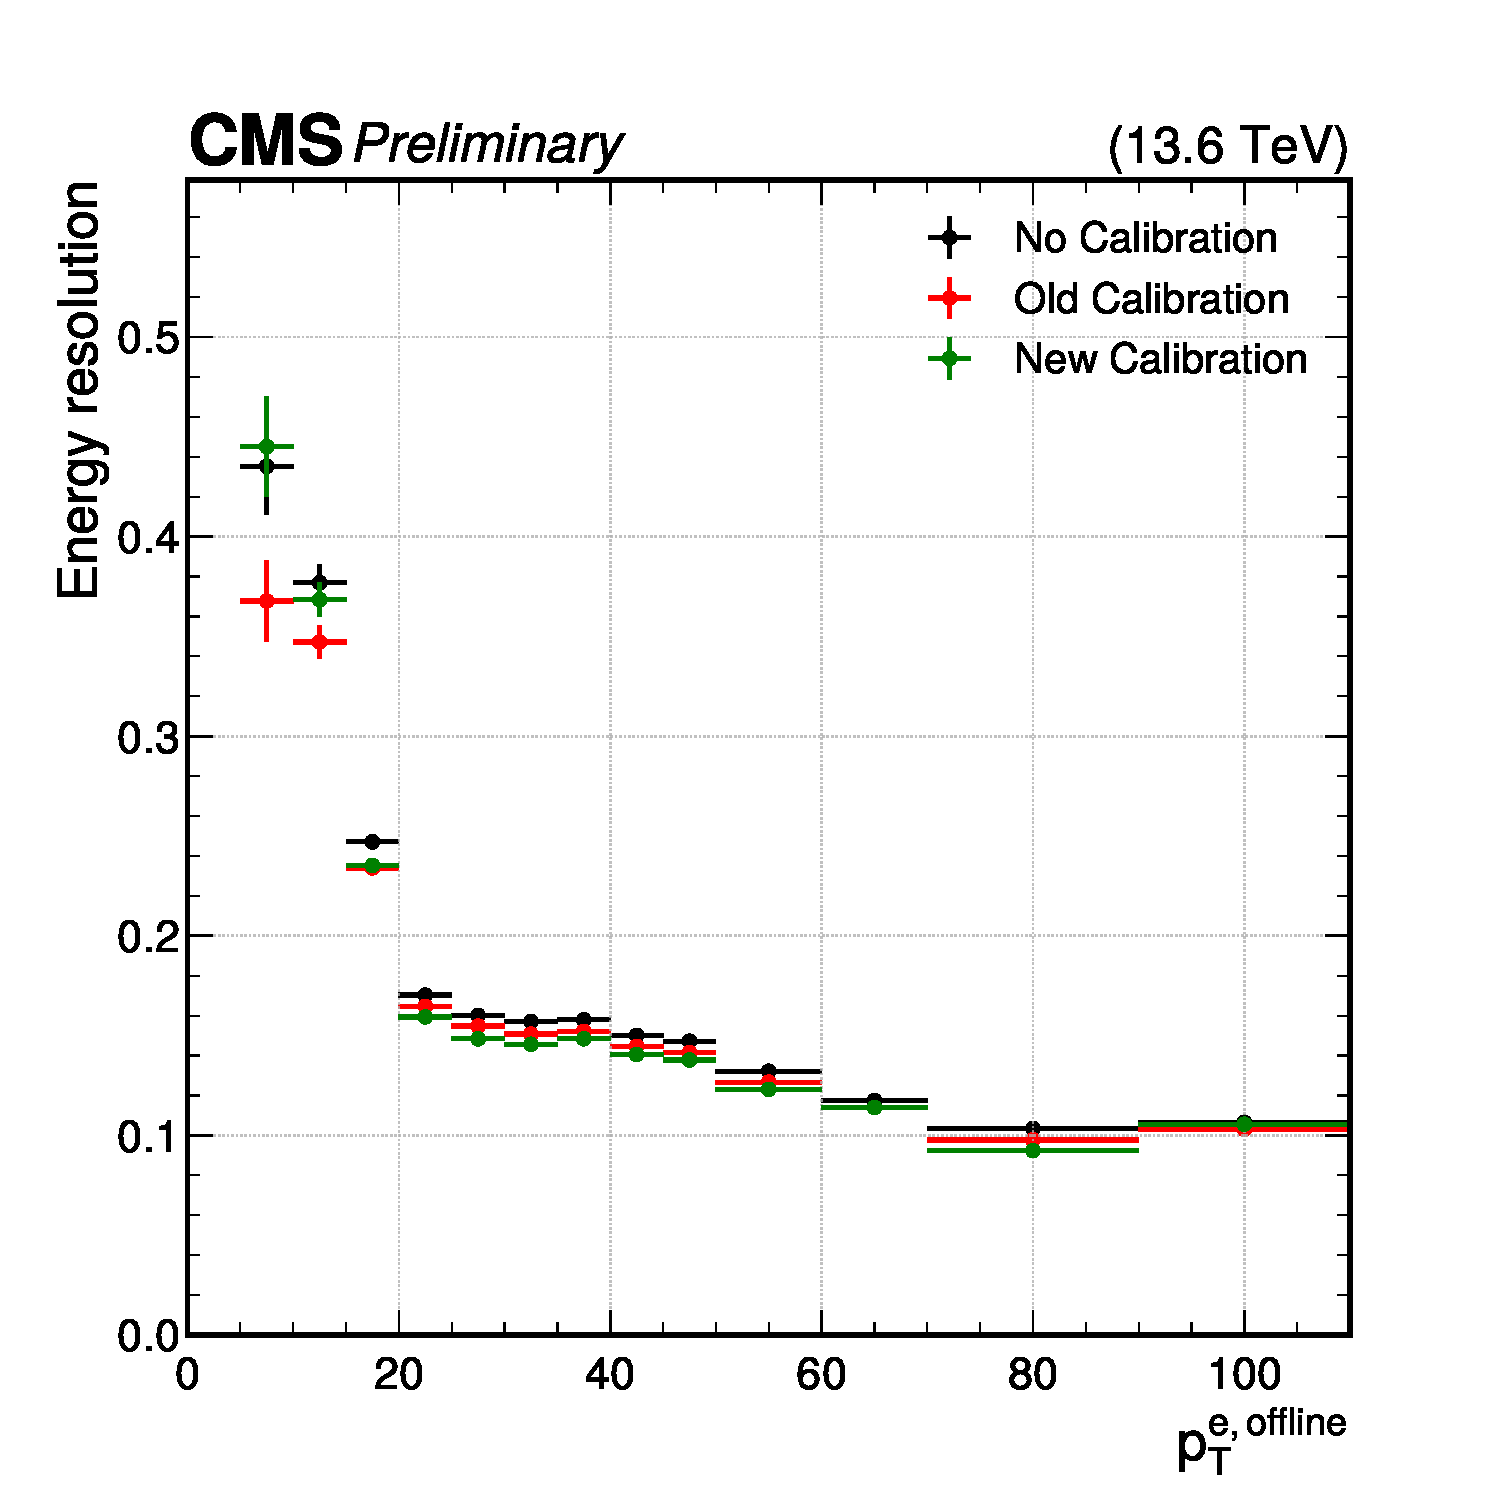
\includegraphics[width=0.5\linewidth]{Figures/L1TP/JAX_Performance/resolution_ptBins__ele.pdf}}
    \subfloat[]{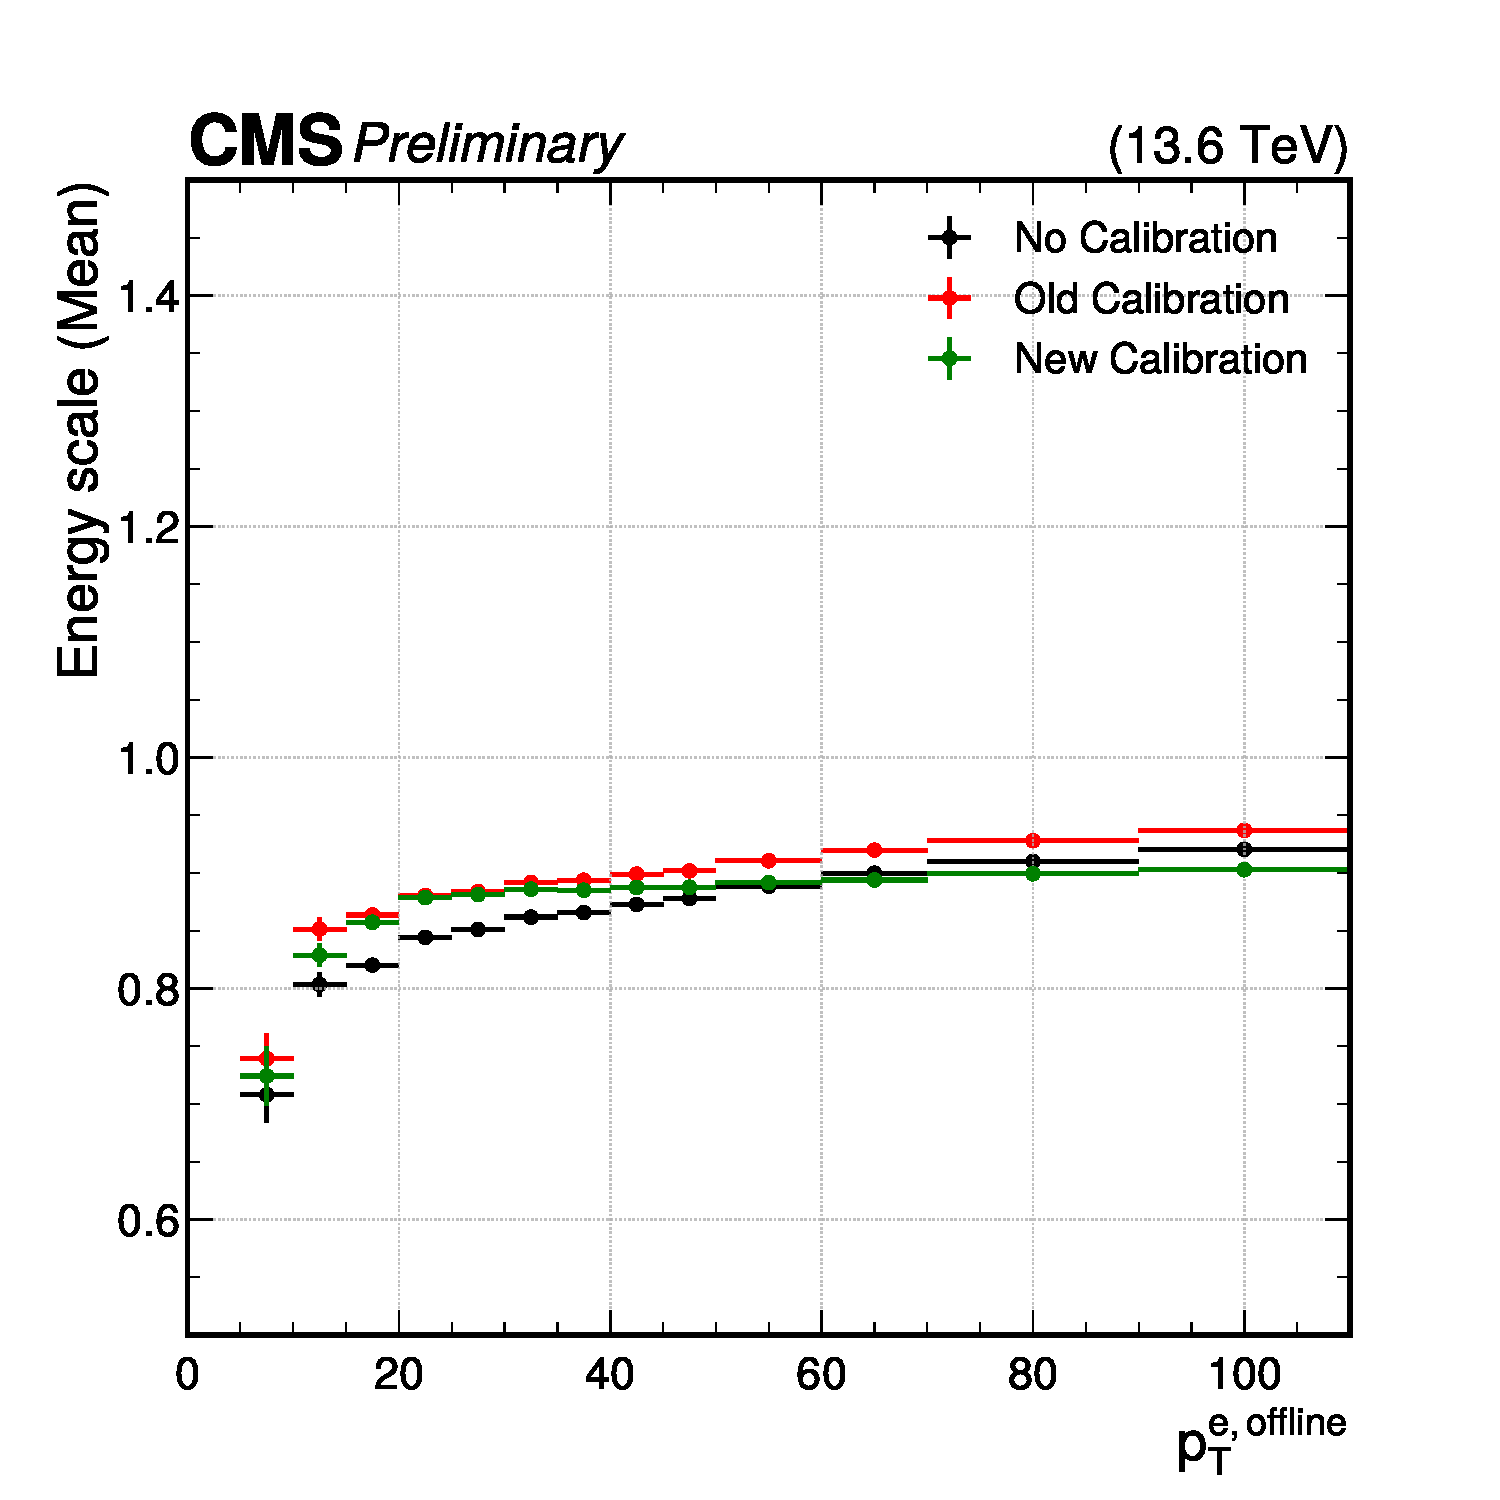
\includegraphics[width=0.5\linewidth]{Figures/L1TP/JAX_Performance/scale_ptBins__ele.pdf}}
    \caption{}
    \label{fig:JAX_ECAL_Response}
\end{figure}

\begin{figure}
    \centering
    \subfloat[]{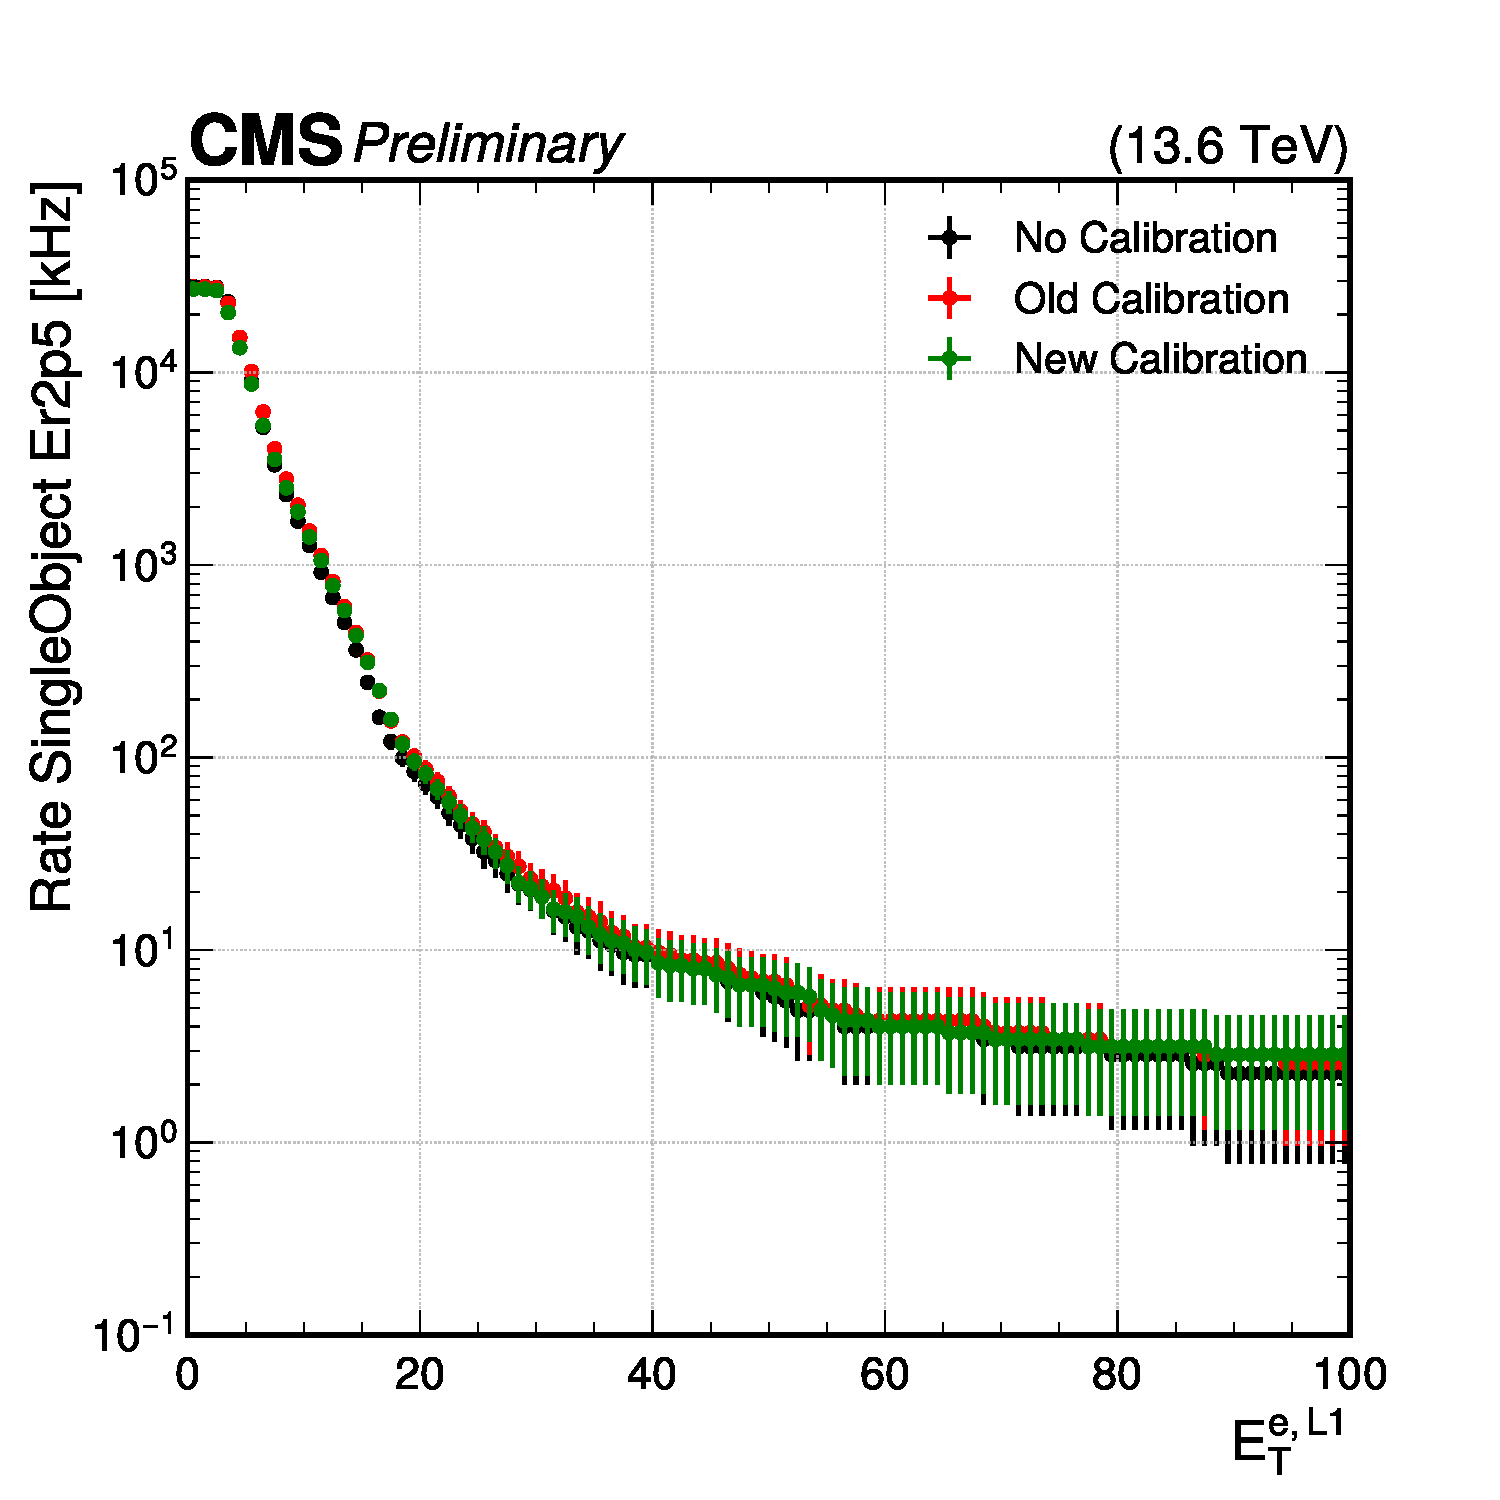
\includegraphics[width=0.5\linewidth]{Figures/L1TP/JAX_Performance/rate_ObjEr2p5__ele.pdf}}
    
    \subfloat[]{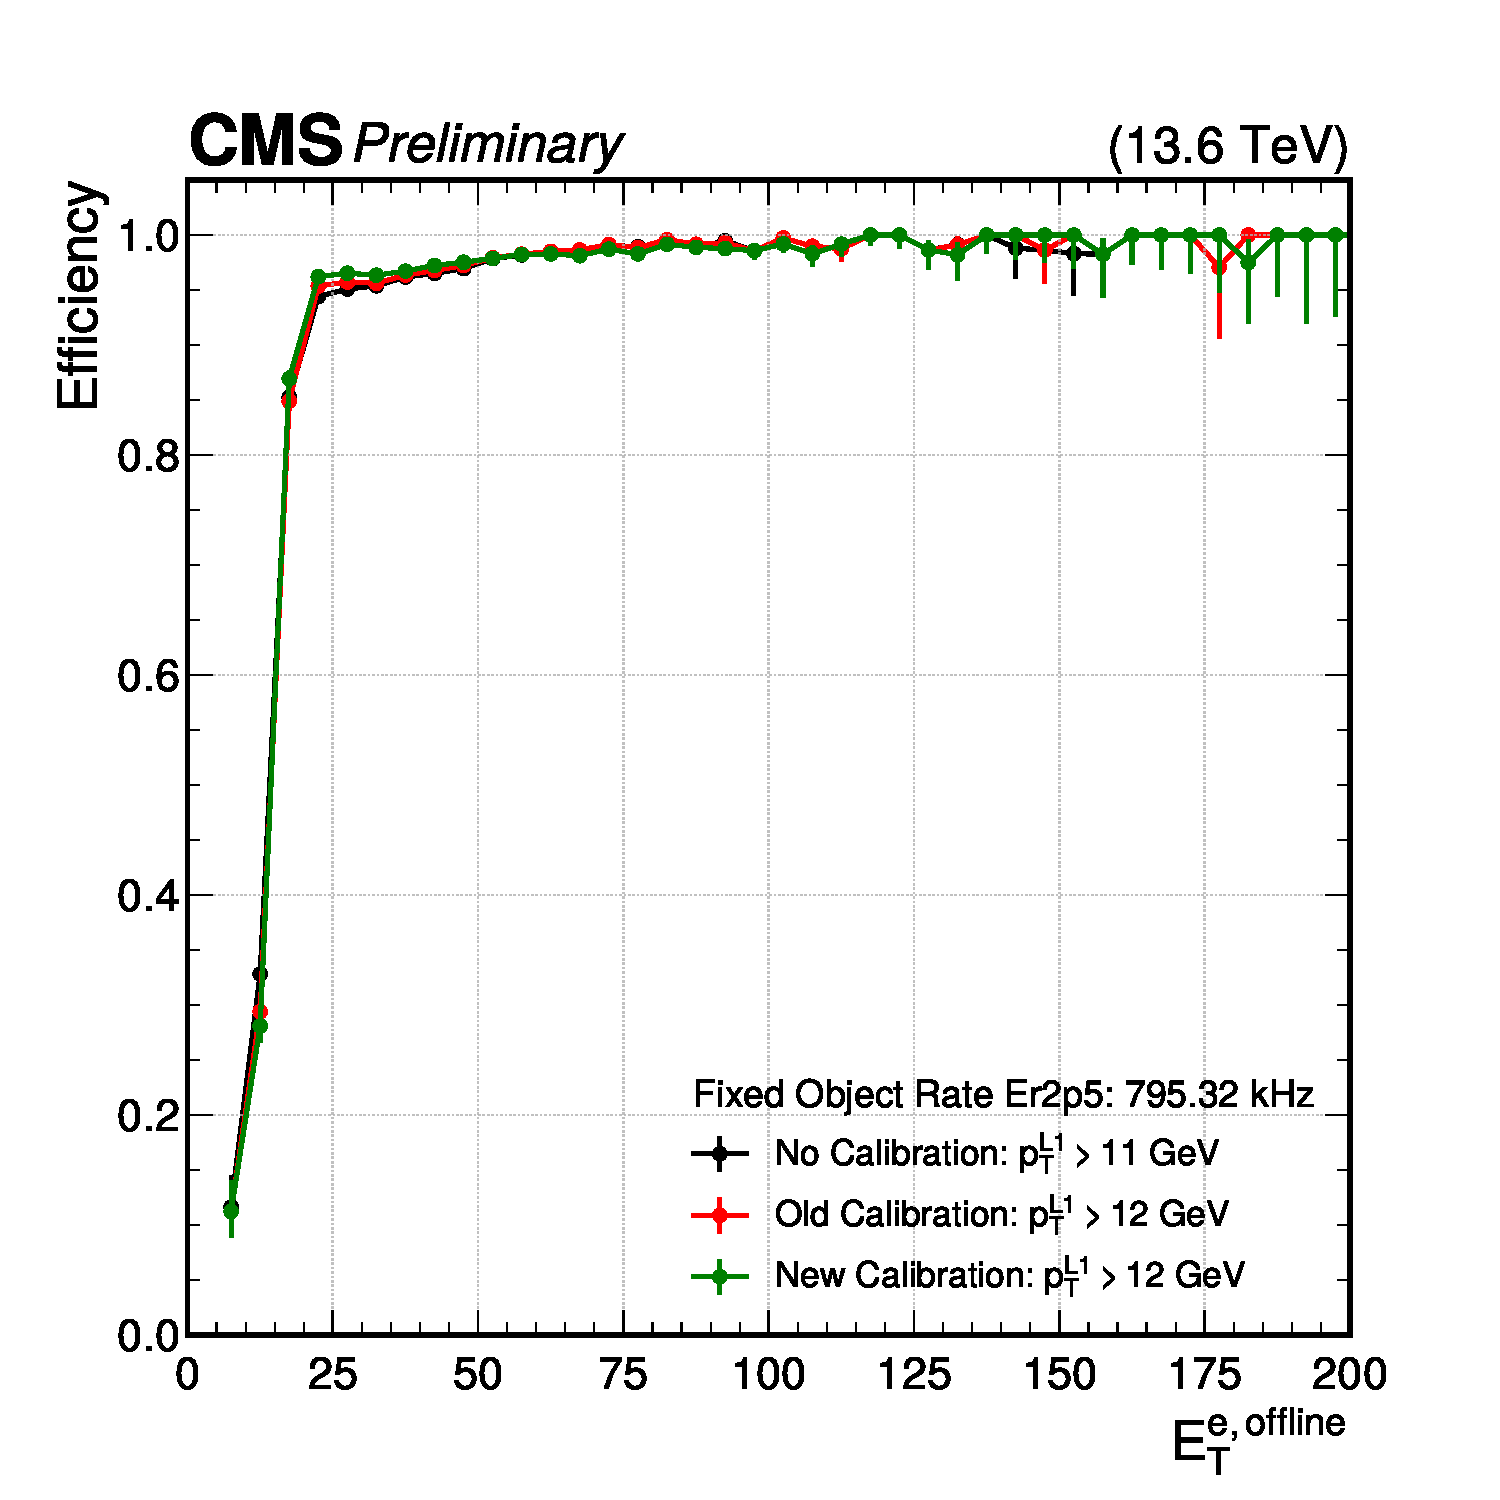
\includegraphics[width=0.5\linewidth]{Figures/L1TP/NN_Performance/turnon_fixedObjRateEr2p5_12__ele.pdf}}
    \subfloat[]{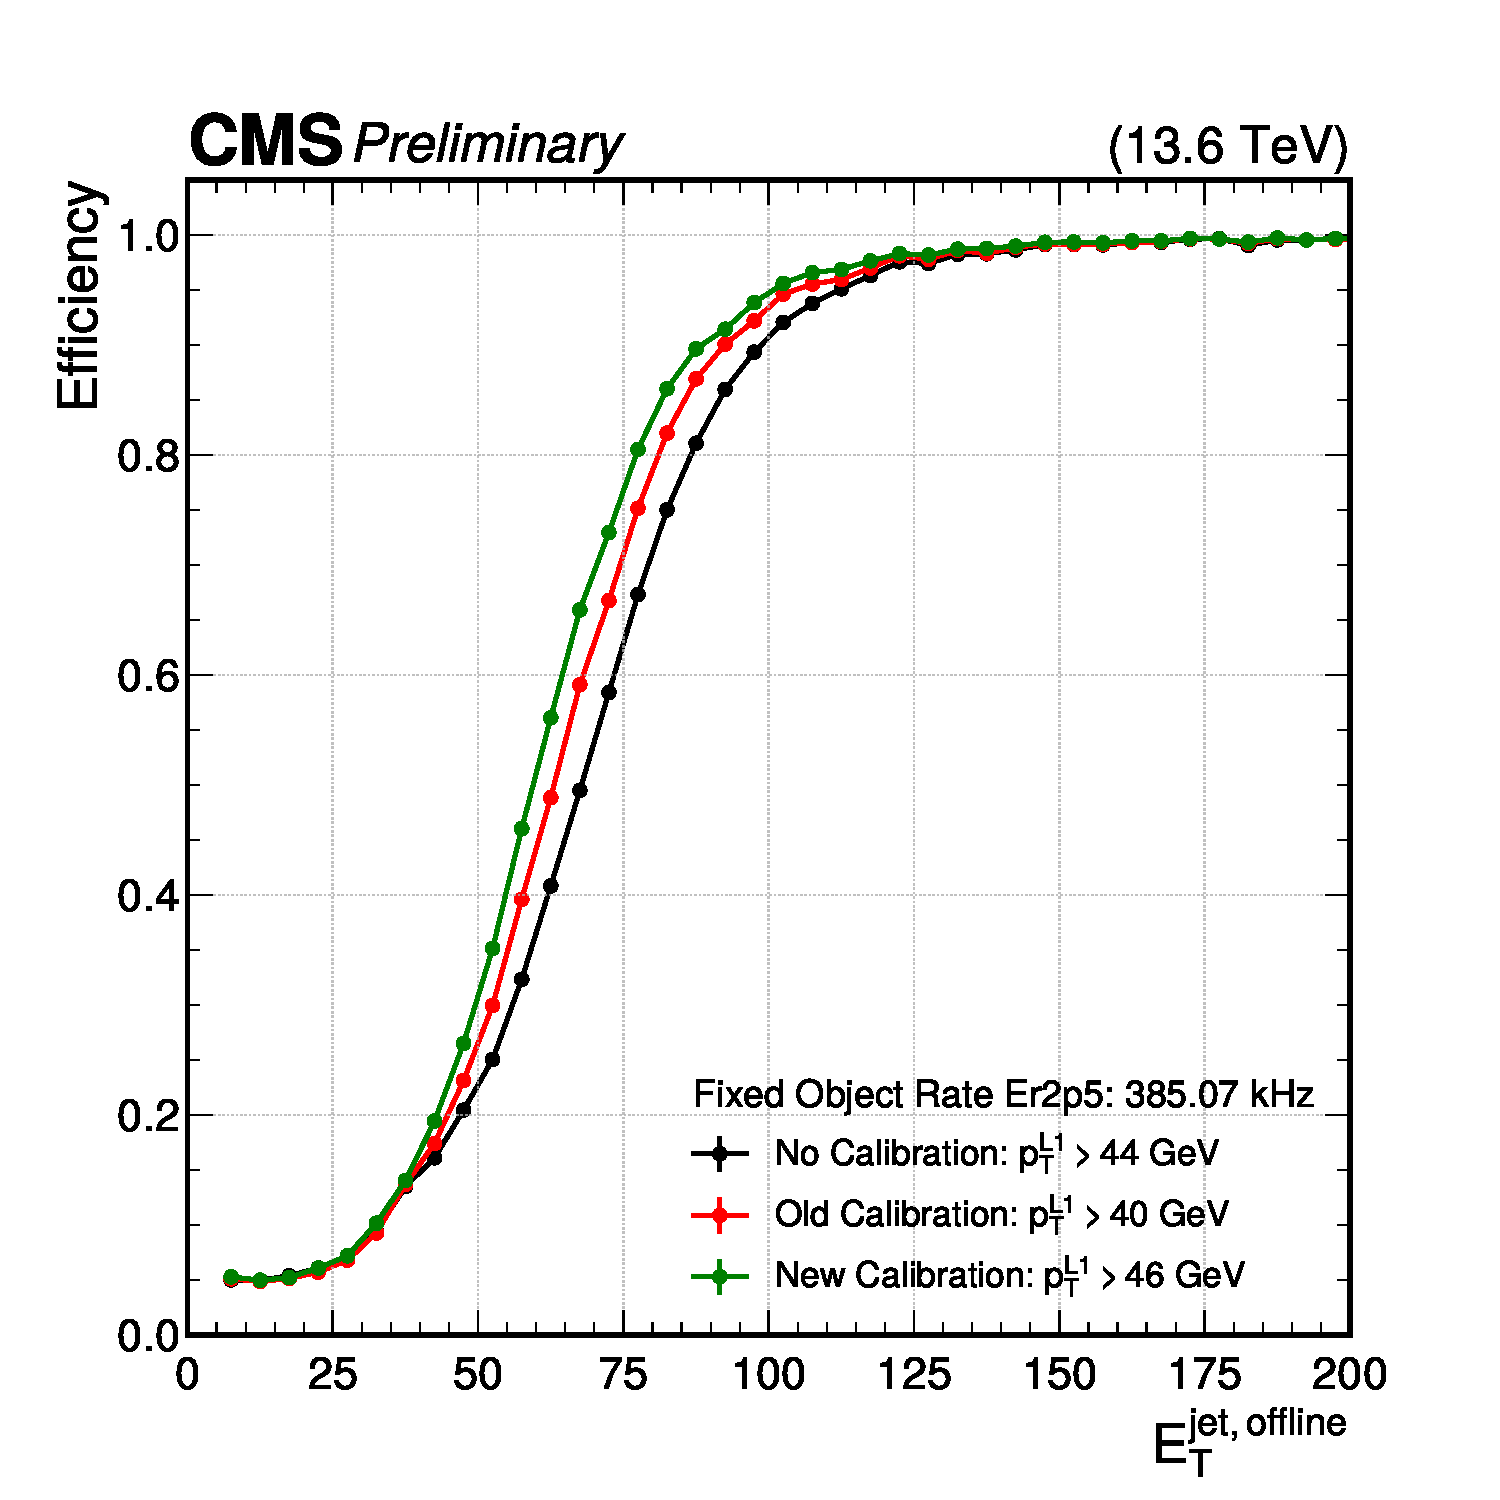
\includegraphics[width=0.5\linewidth]{Figures/L1TP/JAX_Performance/turnon_fixedObjRateEr2p5_40__jet.pdf}}
    \caption{}
    \label{fig:JAX_ECAL_TurnOn}
\end{figure}

\begin{figure}
    \centering
    \subfloat[]{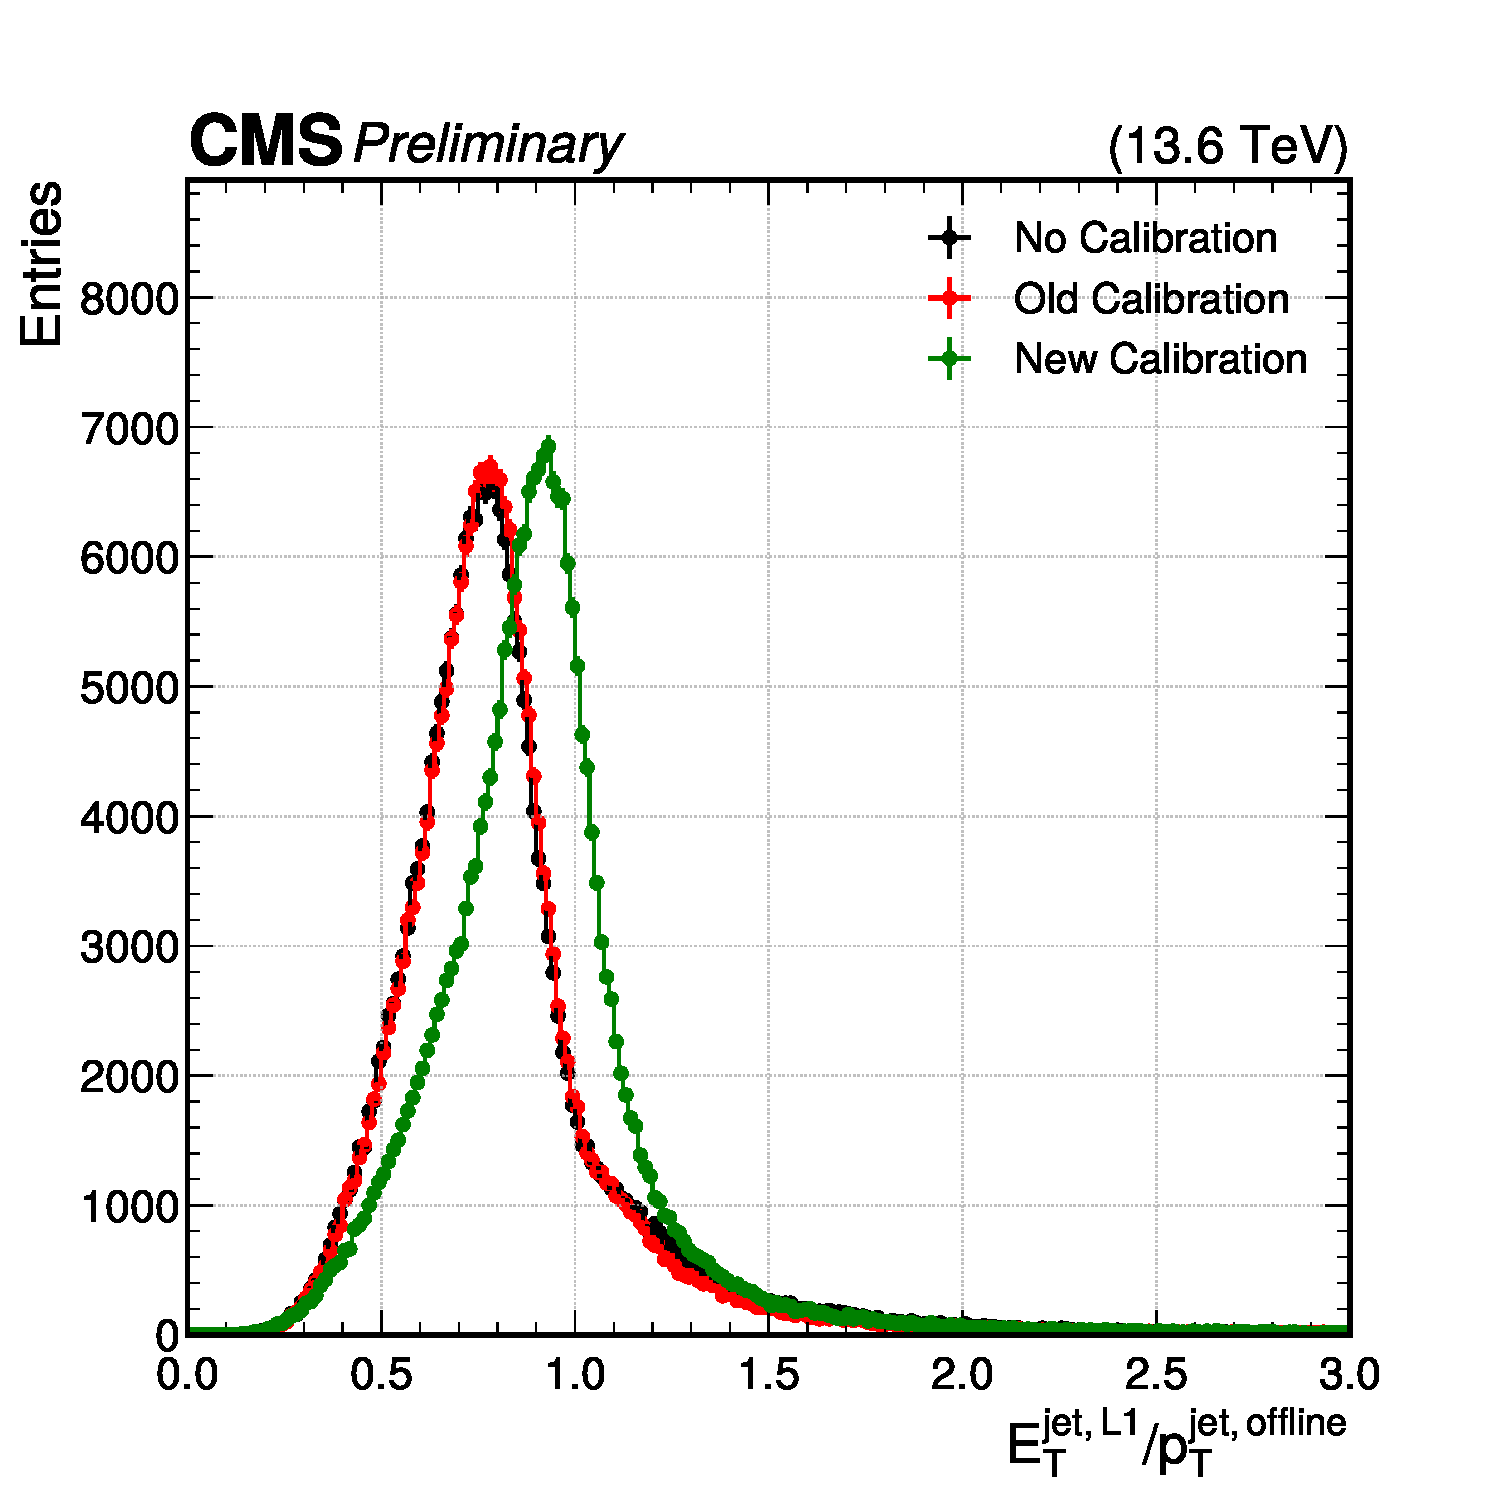
\includegraphics[width=0.5\linewidth]{Figures/L1TP/JAX_Performance/response_inclusive__jet.pdf}}
    
    \subfloat[]{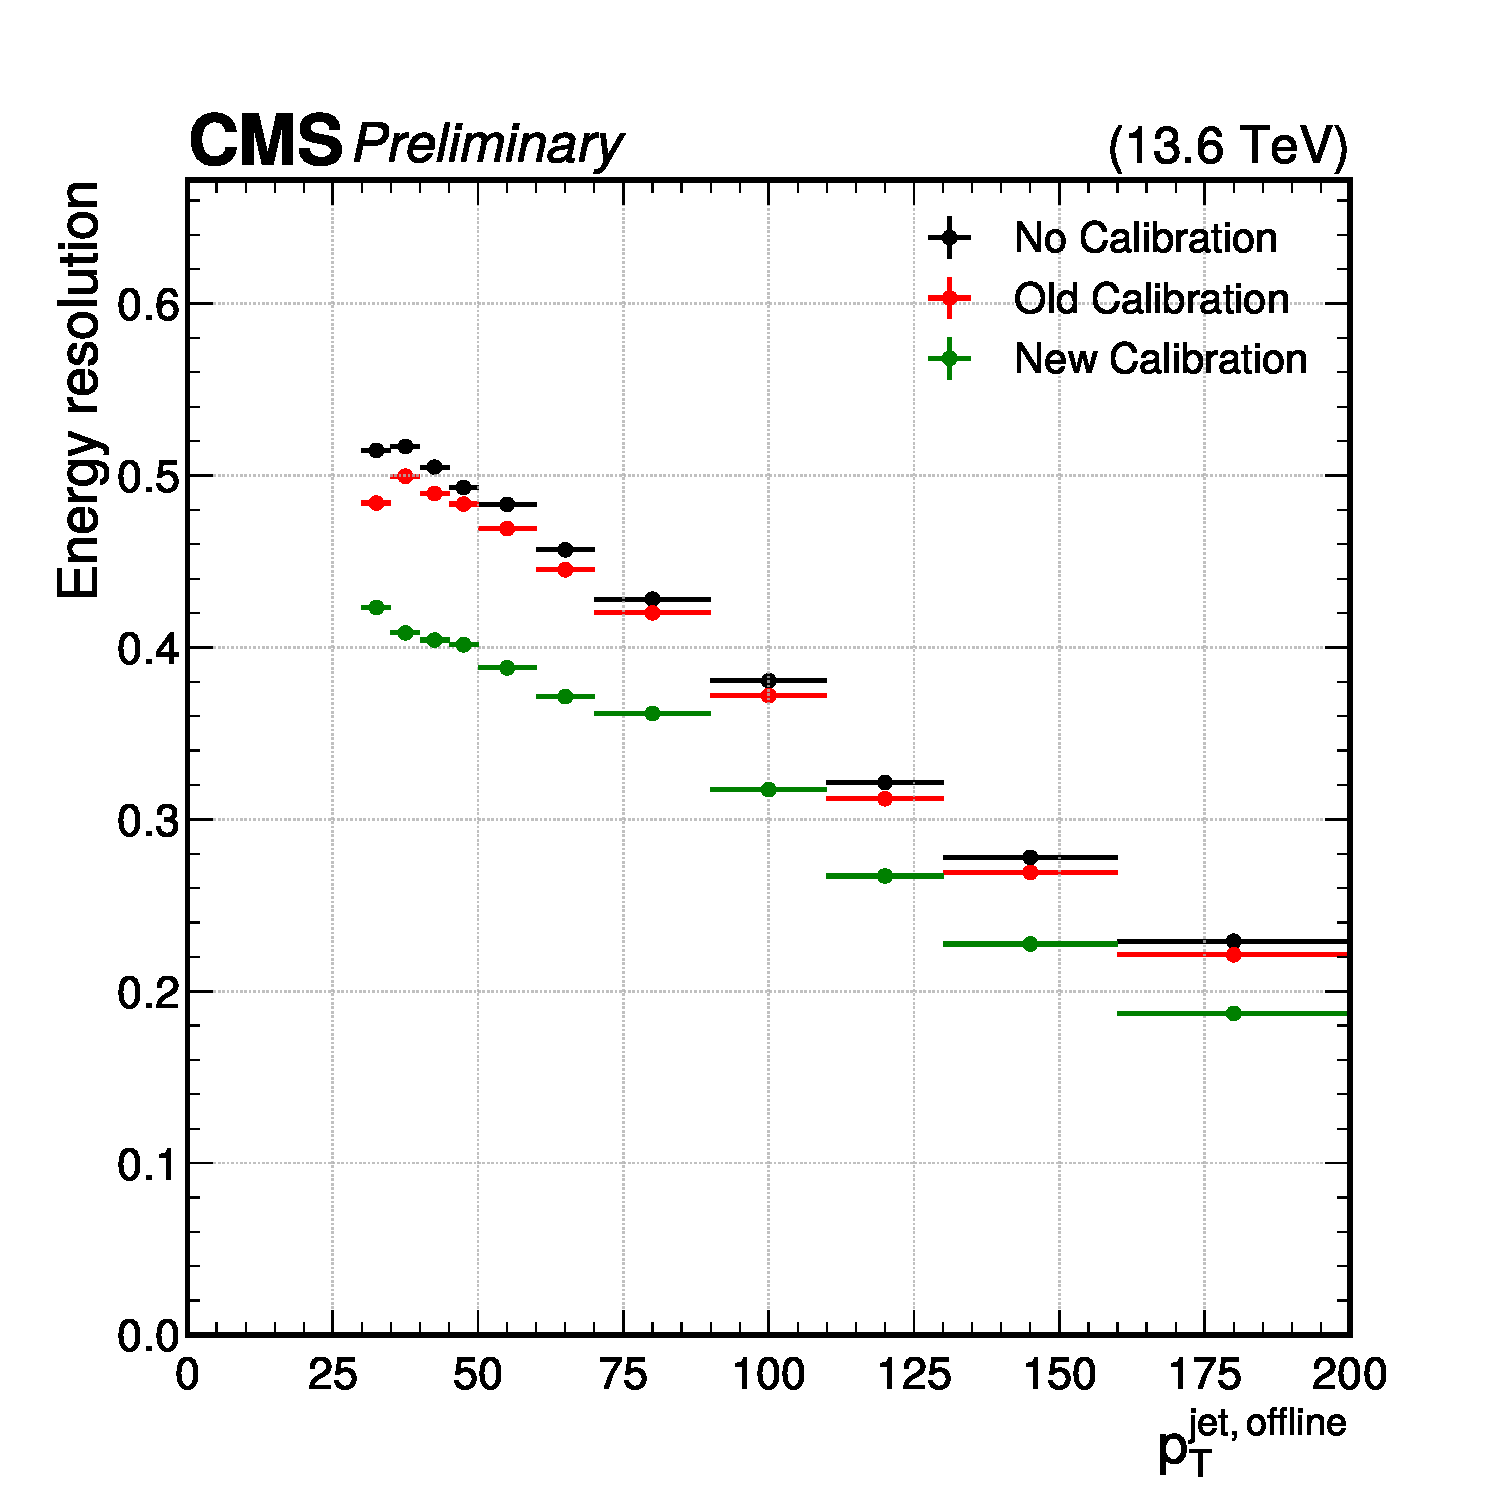
\includegraphics[width=0.5\linewidth]{Figures/L1TP/JAX_Performance/resolution_ptBins__jet.pdf}}
    \subfloat[]{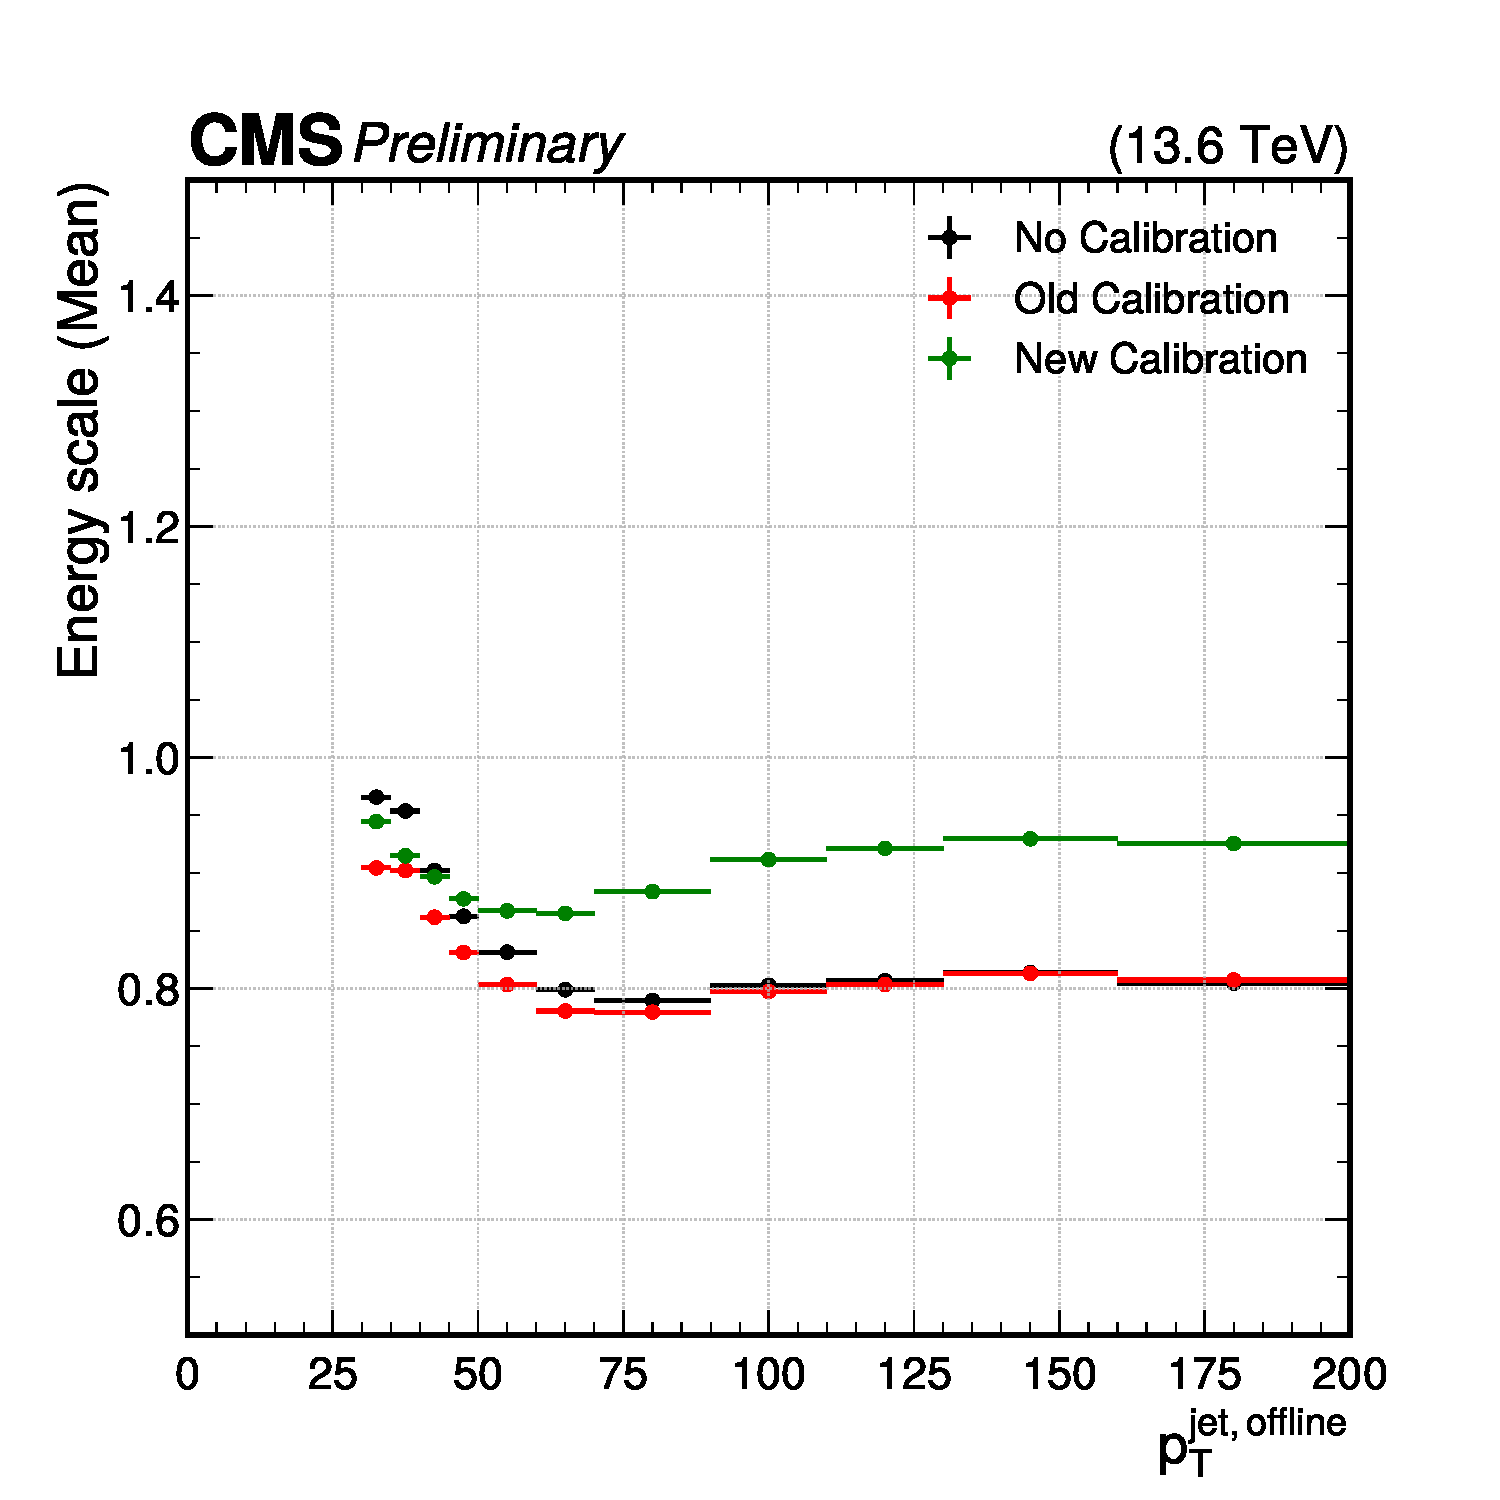
\includegraphics[width=0.5\linewidth]{Figures/L1TP/JAX_Performance/scale_ptBins__jet.pdf}}
    \caption{}
    \label{fig:JAX_HCAL_Response}
\end{figure}

\begin{figure}
    \centering
    \subfloat[]{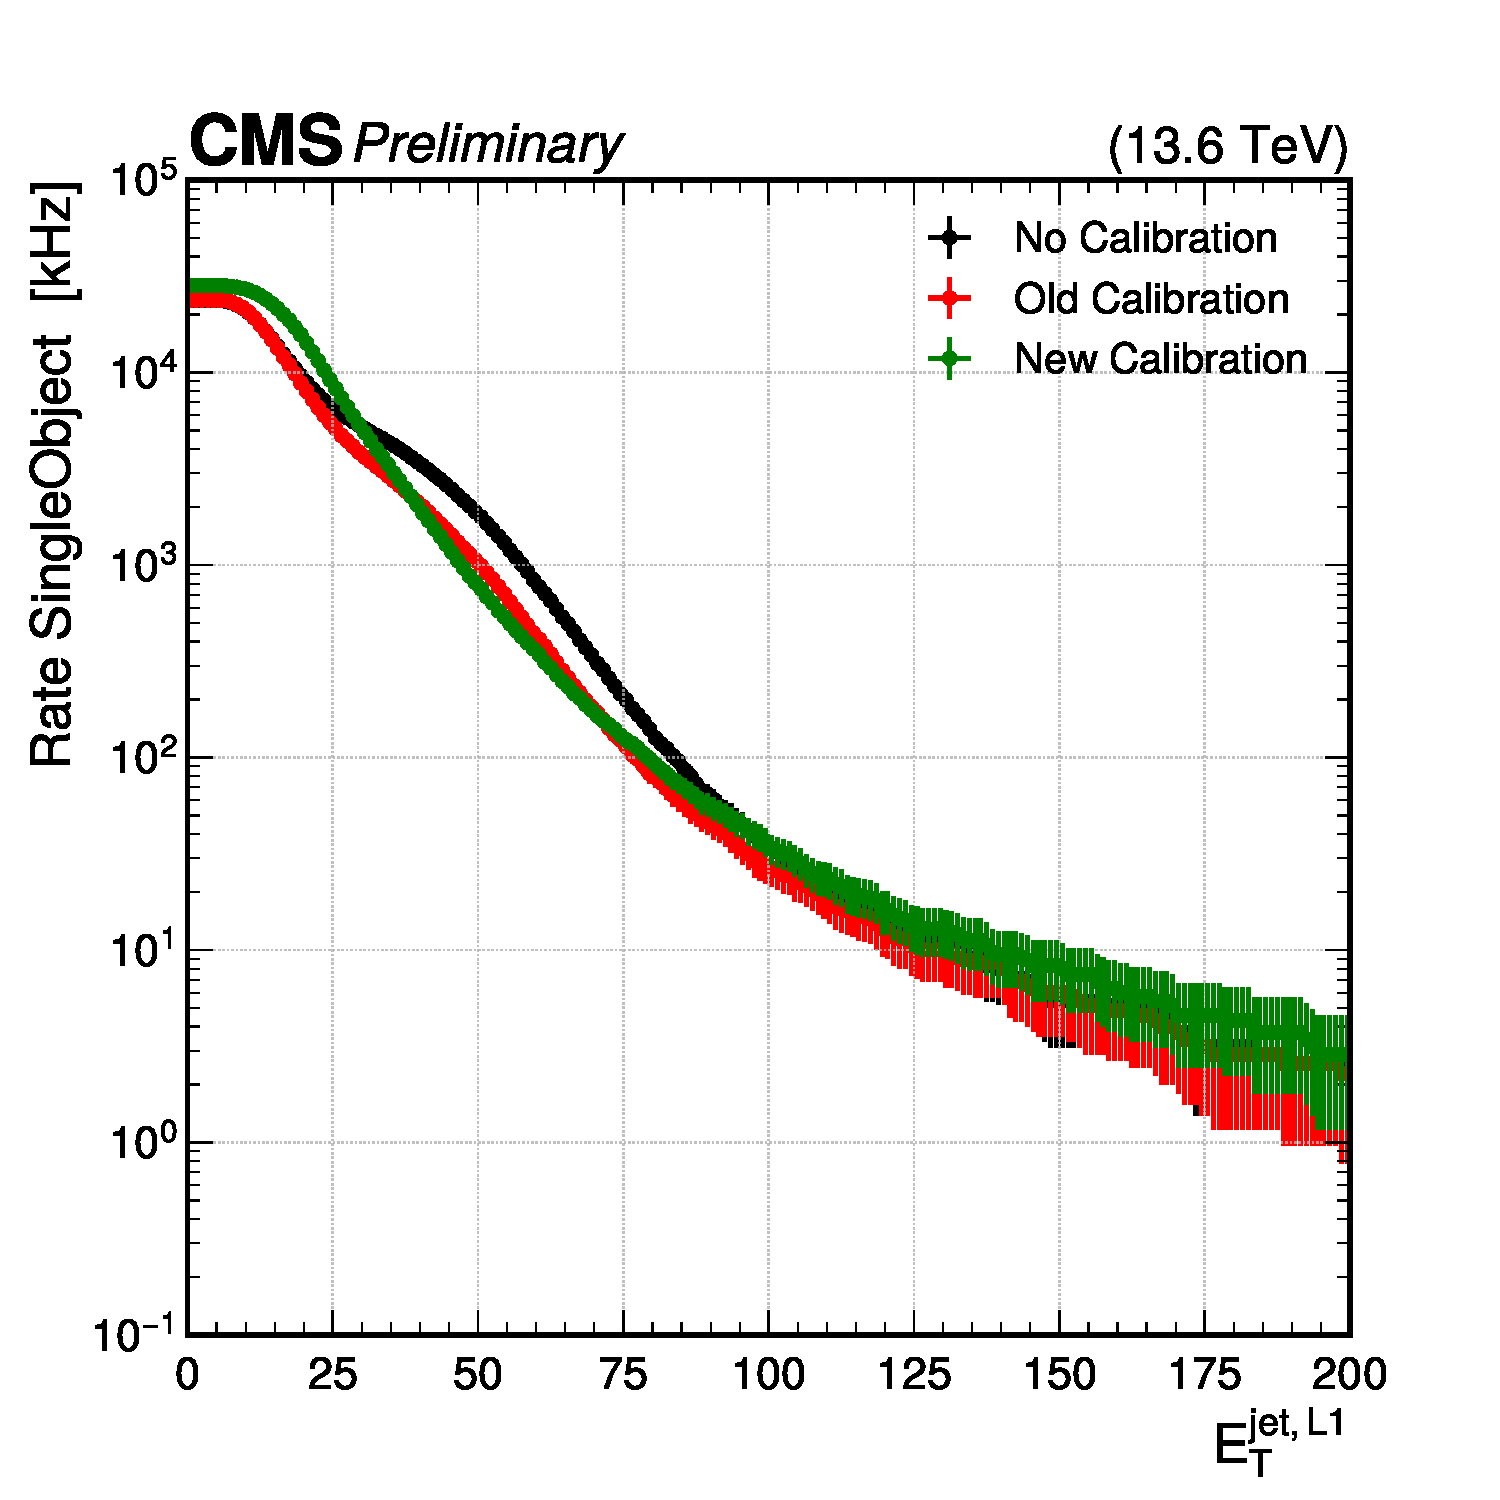
\includegraphics[width=0.5\linewidth]{Figures/L1TP/JAX_Performance/rate_Obj__jet.pdf}}
    
    \subfloat[]{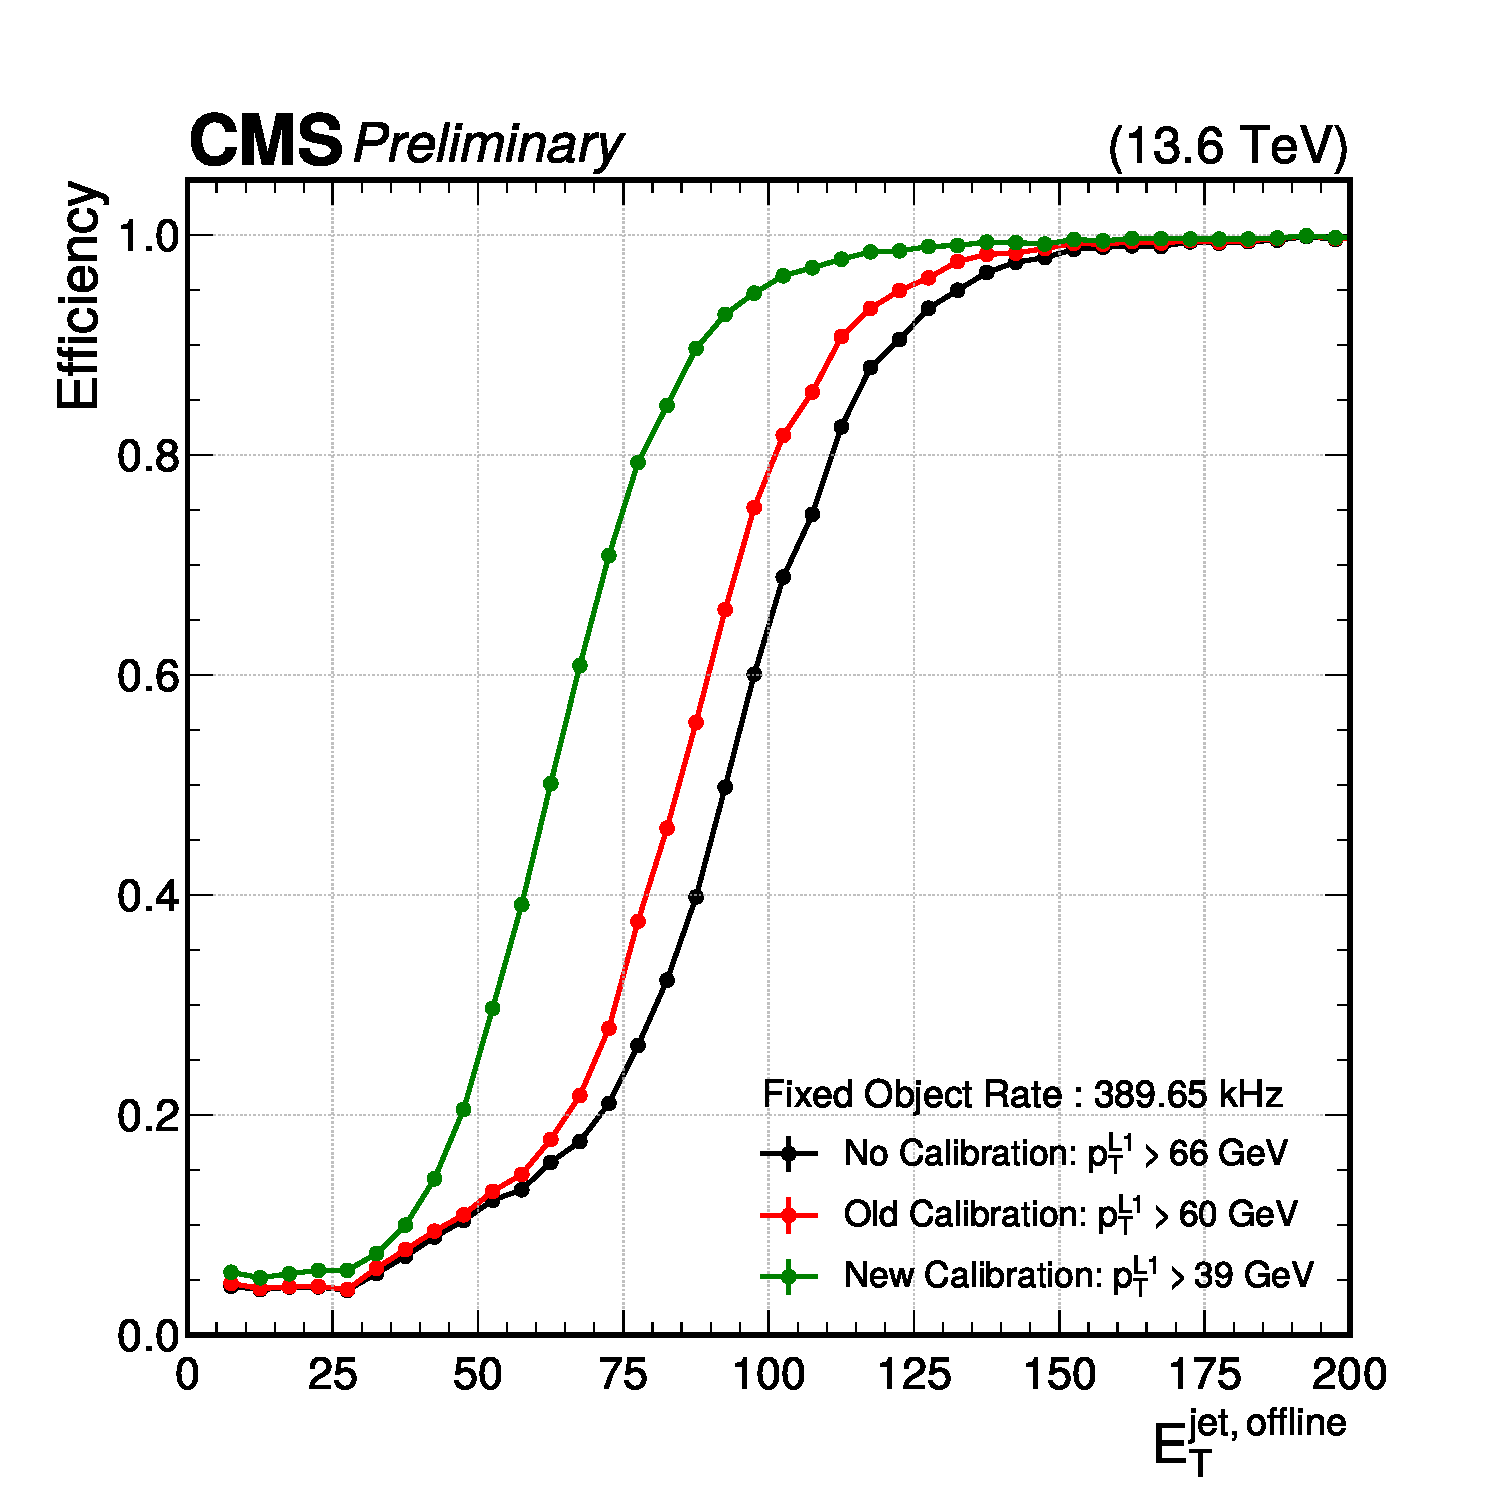
\includegraphics[width=0.5\linewidth]{Figures/L1TP/NN_Performance/turnon_fixedObjRate_60__jet.pdf}}
    \subfloat[]{\includegraphics[width=0.5\linewidth]{Figures/L1TP/JAX_Performance/turnon_fixedObjRate_80__jet.pdf}}
    \caption{}
    \label{fig:JAX_HCAL_TurnOn}
\end{figure}

\begin{figure}
    \centering
    \subfloat[]{\includegraphics[width=0.5\linewidth]{Figures/L1TP/JAX_Performance/rate_ObjEr2p5__jet.pdf}}
    
    \subfloat[]{\includegraphics[width=0.5\linewidth]{Figures/L1TP/NN_Performance/turnon_fixedObjRateEr2p5_40__jet.pdf}}
    \subfloat[]{\includegraphics[width=0.5\linewidth]{Figures/L1TP/JAX_Performance/turnon_fixedObjRateEr2p5_60__jet.pdf}}
    \caption{}
    \label{fig:JAX_HCAL_TurnOn_Er2p5}
\end{figure}

\section{Future applications} % 1/7

\section*{Summary} % 1/7 + introduction and revision